% Für eine Kompilation des Skripts "from scratch" bitte die Kompilationsreihenfolge aus der make.sh anwenden.
% Während Bearbeitungen genügt die ein- oder zweimalige Kompilation mit pdflatex.

% An zukünftige Editoren: Wenn bei der Bearbeitung des Skripts Schwierigkeiten oder Fragen auftreten, wendet euch gerne an mich per Email: lukathome@gmx.net
% Bitte schaut einmal im Readme-Ordner in die "Für Skript-Editoren.txt". Darin findet ihr Bemerkungen zur Dokumentstruktur und Tipps zum TeXen.

\documentclass{VK-Skript}

% Pdf-Metadaten
\hypersetup{
    pdftitle={Skript zum Mathematischen Vorkurs},
    pdfauthor={Luka Thomé, Fachschaft MathPhysInfo Heidelberg}
}

% ====================================================================
% <<Zahlbereiche>>
% ====================================================================

\newcommand{\N}{\mathbb N}
\newcommand{\Z}{\mathbb Z}
\newcommand{\Q}{\mathbb Q}
\newcommand{\R}{\mathbb R}
\newcommand{\C}{\mathbb C}

% ====================================================================
% <<Abkürzungen>>
% ====================================================================

\newcommand{\id}{\mathrm{id}} % Identität
\newcommand{\inv}{\mathrm{inv}} % invers
\newcommand{\ev}{\mathrm{ev}} % evaluate
\newcommand{\op}{\mathrm{op}} % opposite


\DeclareMathOperator{\Abb}{Abb} % Menge der Abbildungen
\DeclareMathOperator{\Ch}{Ch} % Komplexe
\DeclareMathOperator{\codom}{codom} % Wertebereich
\DeclareMathOperator{\coim}{coim} % Kobild
\DeclareMathOperator{\dom}{dom} % Definitionsbereich
\DeclareMathOperator{\ggT}{ggT} % größter gemeinsamer Teiler
\DeclareMathOperator{\graph}{graph} % Graph einer Funktion
\DeclareMathOperator{\im}{im} % Bild
\DeclareMathOperator{\kgV}{kgV} % kleinstes gemeinsames Vielfaches
\DeclareMathOperator{\Rel}{Rel} % Relationen
\DeclareMathOperator{\res}{res} % Restriktion
\DeclareMathOperator{\sgn}{sgn} % Signum
\DeclareMathOperator{\Sh}{Sh} % Garben


\newcommand{\TODO}{\colorbox{cyan}{\textup{TODO}}} % Todo-Kürzel

% ====================================================================
% <<Kategorien>>
% ====================================================================

\newcommand{\Grp}{\mathsf{Grp}} % Gruppen
\newcommand{\Mon}{\mathsf{Mon}} % Monoide
\newcommand{\Pos}{\mathsf{Pos}} % Posets (= geordnete Mengen)
\newcommand{\Set}{\mathsf{Set}} % Mengen

% ====================================================================
% <<Alphabete>>
% ====================================================================

% \mathcal alphabet capital
\newcommand{\calA}{\mathcal A}
\newcommand{\calB}{\mathcal B}
\newcommand{\calC}{\mathcal C}
\newcommand{\calD}{\mathcal D}
\newcommand{\calE}{\mathcal E}
\newcommand{\calF}{\mathcal F}
\newcommand{\calG}{\mathcal G}
\newcommand{\calH}{\mathcal H}
\newcommand{\calI}{\mathcal I}
\newcommand{\calJ}{\mathcal J}
\newcommand{\calK}{\mathcal K}
\newcommand{\calL}{\mathcal L}
\newcommand{\calM}{\mathcal M}
\newcommand{\calN}{\mathcal N}
\newcommand{\calO}{\mathcal O}
\newcommand{\calP}{\mathcal P}
\newcommand{\calQ}{\mathcal Q}
\newcommand{\calR}{\mathcal R}
\newcommand{\calS}{\mathcal S}
\newcommand{\calT}{\mathcal T}
\newcommand{\calU}{\mathcal U}
\newcommand{\calV}{\mathcal V}
\newcommand{\calW}{\mathcal W}
\newcommand{\calX}{\mathcal X}
\newcommand{\calY}{\mathcal Y}
\newcommand{\calZ}{\mathcal Z}

% \mathbb alphabet capital
\newcommand{\bbA}{\mathbb A}
\newcommand{\bbB}{\mathbb B}
\newcommand{\bbC}{\mathbb C}
\newcommand{\bbD}{\mathbb D}
\newcommand{\bbE}{\mathbb E}
\newcommand{\bbF}{\mathbb F}
\newcommand{\bbG}{\mathbb G}
\newcommand{\bbH}{\mathbb H}
\newcommand{\bbI}{\mathbb I}
\newcommand{\bbJ}{\mathbb J}
\newcommand{\bbK}{\mathbb K}
\newcommand{\bbL}{\mathbb L}
\newcommand{\bbM}{\mathbb M}
\newcommand{\bbN}{\mathbb N}
\newcommand{\bbO}{\mathbb O}
\newcommand{\bbP}{\mathbb P}
\newcommand{\bbQ}{\mathbb Q}
\newcommand{\bbR}{\mathbb R}
\newcommand{\bbS}{\mathbb S}
\newcommand{\bbT}{\mathbb T}
\newcommand{\bbU}{\mathbb U}
\newcommand{\bbV}{\mathbb V}
\newcommand{\bbW}{\mathbb W}
\newcommand{\bbX}{\mathbb X}
\newcommand{\bbY}{\mathbb Y}
\newcommand{\bbZ}{\mathbb Z}

% \mathfrak alphabet 
\newcommand{\fraka}{\mathfrak a}
\newcommand{\frakb}{\mathfrak b}
\newcommand{\frakc}{\mathfrak c}
\newcommand{\frakd}{\mathfrak d}
\newcommand{\frake}{\mathfrak e}
\newcommand{\frakf}{\mathfrak f}
\newcommand{\frakg}{\mathfrak g}
\newcommand{\frakh}{\mathfrak h}
\newcommand{\fraki}{\mathfrak i}
\newcommand{\frakj}{\mathfrak j}
\newcommand{\frakk}{\mathfrak k}
\newcommand{\frakl}{\mathfrak l}
\newcommand{\frakm}{\mathfrak m}
\newcommand{\frakn}{\mathfrak n}
\newcommand{\frako}{\mathfrak o}
\newcommand{\frakp}{\mathfrak p}
\newcommand{\frakq}{\mathfrak q}
\newcommand{\frakr}{\mathfrak r}
\newcommand{\fraks}{\mathfrak s}
\newcommand{\frakt}{\mathfrak t}
\newcommand{\fraku}{\mathfrak u}
\newcommand{\frakv}{\mathfrak v}
\newcommand{\frakw}{\mathfrak w}
\newcommand{\frakx}{\mathfrak x}
\newcommand{\fraky}{\mathfrak y}
\newcommand{\frakz}{\mathfrak z}

% \mathfrak alphabet capital
\newcommand{\frakA}{\mathfrak A}
\newcommand{\frakB}{\mathfrak B}
\newcommand{\frakC}{\mathfrak C}
\newcommand{\frakD}{\mathfrak D}
\newcommand{\frakE}{\mathfrak E}
\newcommand{\frakF}{\mathfrak F}
\newcommand{\frakG}{\mathfrak G}
\newcommand{\frakH}{\mathfrak H}
\newcommand{\frakI}{\mathfrak I}
\newcommand{\frakJ}{\mathfrak J}
\newcommand{\frakK}{\mathfrak K}
\newcommand{\frakL}{\mathfrak L}
\newcommand{\frakM}{\mathfrak M}
\newcommand{\frakN}{\mathfrak N}
\newcommand{\frakO}{\mathfrak O}
\newcommand{\frakP}{\mathfrak P}
\newcommand{\frakQ}{\mathfrak Q}
\newcommand{\frakR}{\mathfrak R}
\newcommand{\frakS}{\mathfrak S}
\newcommand{\frakT}{\mathfrak T}
\newcommand{\frakU}{\mathfrak U}
\newcommand{\frakV}{\mathfrak V}
\newcommand{\frakW}{\mathfrak W}
\newcommand{\frakX}{\mathfrak X}
\newcommand{\frakY}{\mathfrak Y}
\newcommand{\frakZ}{\mathfrak Z}
 % Kürzel für Mathe

\newacronym{sym:N}{$\N$}{Menge der natürlichen Zahlen (siehe \cref{natzahlen})}
\newacronym{sym:Z}{$\Z$}{Menge der ganzen Zahlen}
\newacronym{sym:Q}{$\Q$}{Menge der rationalen Zahlen}
\newacronym{sym:R}{$\R$}{Menge der reellen Zahlen}
\newacronym{sym:C}{$\C$}{Menge der komplexen Zahlen}
\newacronym{sym:nZ}{$n\Z$}{Menge aller ganzzahligen Vielfachen von $n$}


\newacronym{sym:perdef}{\quad\\[0.5em] $:=$}{Per Definition gleich} % Das \quad ist zum Einfügen eines Phantom-Zeilenabstands (sorry, kriegs nicht besser hin)
\newacronym{sym:perdefiff}{$:\Leftrightarrow$}{Per Definition äquivalent zu}
\newacronym{sym:land}{$\land$}{Und}
\newacronym{sym:lor}{$\lor$}{Oder}
\newacronym{sym:neg}{$\neg$}{Aussagenlogische Negation}
\newacronym{sym:implikation}{$\rightarrow$\quad bzw.\quad $\Rightarrow$}{Aussagenlogische Implikation}
\newacronym{sym:iff}{$\leftrightarrow$\quad bzw.\quad $\Leftrightarrow$}{Aussagenlogische Äquivalenz}
\newacronym{sym:forall}{$\forall$}{Allquantor}
\newacronym{sym:exists}{$\exists$}{Existenzquantor}


\newacronym{sym:in}{\quad\\[0.5em] $\in$}{Element}
\newacronym{sym:subseteq}{$\subseteq$}{Teilmenge}
\newacronym{sym:subsetneq}{$\subsetneq$}{Echte Teilmenge}
\newacronym{sym:emptyset}{$\emptyset$}{Leere Menge}
\newacronym{sym:potenzmenge}{$\calP(X)$}{Potenzmenge von $X$}
\newacronym{sym:familie}{$(a_i)_{i\in I}$}{Durch die Menge $I$ indizierte Familie von Objekten $a_i$}
\newacronym{sym:mengenpotenz}{$M^I$}{Menge der durch $I$ indizierten Familien mit Einträgen aus $M$}
\newacronym{sym:matrizenmenge}{$M^{n\times m}$}{Menge der $(n\times m)$-Matrizen mit Einträgen aus $M$}
\newacronym{sym:paar}{$(x,y)$}{Geordnetes Paar bestehend aus zwei Objekten $x,y$}
\newacronym{sym:cap}{$\cap$}{Durchschnitt von Mengen}
\newacronym{sym:cup}{$\cup$}{Vereinigung von Mengen}
\newacronym{sym:setminus}{$\setminus$}{Differenz zweier Mengen}
\newacronym{sym:komplement}{$M^c$}{Komplement von $M$ (in einer fixierten Obermenge)}
\newacronym{sym:times}{$\times$}{Kartesisches Produkt}
\newacronym{sym:sqcup}{$\sqcup$}{Disjunkte Vereinigung}


\newacronym{sym:funktion}{\quad\\[0.5em] $f:X\to Y$\quad bzw.\quad $X\xrightarrow{f} Y$}{$f$ ist eine Abbildung von $X$ nach $Y$}
\newacronym{sym:zuordnung}{$x\mapsto t(x)$}{Dem Objekt $x$ wird das Objekt $t(x)$ zugeordnet}
\newacronym{sym:funktionswert}{$f(x)$}{Funktionswert von $f$ an der Stelle $x$}
\newacronym{sym:abb}{$\Abb(X,Y)$}{Menge der Abbildungen von $X$ nach $Y$}
\newacronym{sym:circ}{$\circ$}{Verkettung von Abbildungen}
\newacronym{sym:id}{$\id_X$}{Identität auf $X$}
\newacronym{sym:inklusion}{$\iota: U\hookrightarrow X$}{Inklusion der Teilmenge $U\subseteq X$}
\newacronym{sym:faser}{$f^{-1}(x)$}{Faser von $x$ oder aber Funktionswert unter der inversen Abbildung (sofern diese existiert)}
\newacronym{sym:im}{$\im(f)$}{Bild von $f$}
\newacronym{sym:urbild}{$f^{-1}(B)$}{Urbild von $B$ unter $f$}
\newacronym{sym:bild}{$f(A)$}{Bild von $A$ unter $f$}
\newacronym{sym:domres}{$f\vert_A$}{Einschränkung von $f$ im Definitionsbereich}
\newacronym{sym:codomres}{$f\vert^A$}{Einschränkung von $f$ im Wertebereich}


\newacronym{sym:teilt}{\quad\\[0.5em] $n\mid m$}{$n$ teilt $m$}
\newacronym{sym:le}{$\le$}{Generisches Zeichen für eine Ordnungsrelation}
\newacronym{sym:min}{$\min$}{Minimum, kleinstes Element einer geordneten Menge}
\newacronym{sym:max}{$\max$}{Maximum, größtes Element einer geordneten Menge}
\newacronym{sym:inf}{$\inf$}{Infimum, größte untere Schranke}
\newacronym{sym:sup}{$\sup$}{Supremum, kleinste obere Schranke}
\newacronym{sym:intervall}{$(a,b),\ [a,b],\ (a,b],\ [a,b)$}{Offenes, abgeschlossenes und halboffene Intervalle mit Endpunkten $a$ und $b$}
\newacronym{sym:aequiklasse}{$[x]$\quad bzw.\quad $\bar x$}{Äquivalenzklasse von $x$ bzgl. einer Äquivalenzrelation}
\newacronym{sym:faktormenge}{$X/{\sim}$}{Faktormenge modulo $\sim$}
\newacronym{sym:projektion}{$\pi:X\twoheadrightarrow X/{\sim}$}{Projektion auf die Faktormenge $X/{\sim}$}


\newacronym{sym:addinv}{\quad\\[0.5em] $-x$}{Additiv Inverses von $x$}
\newacronym{sym:multinv}{$x^{-1}$}{Multiplikativ Inverses von $x$}
\newacronym{sym:sum}{$\sum\limits_{k=m}^n a_k$}{Summe der $a_m,\dots , a_n$}
\newacronym{sym:prod}{$\prod\limits_{k=m}^n a_k$}{Produkt der $a_m,\dots , a_n$}
\newacronym{sym:einheitengruppe}{$M^\times$}{Einheitengruppe von $M$}
\newacronym{sym:symgruppe}{$S_n$}{$n$-te symmetrische Gruppe}


\newacronym{sym:Rdach}{\quad\\[0.5em] $\bar \R$}{Um $\pm\infty$ erweiterte reelle Zahlen}
\newacronym{sym:betrag}{$\vert x\vert$}{Betrag von $x$}
\newacronym{sym:sgn}{$\sgn(x)$}{Vorzeichen von $x$}
\newacronym{sym:abstand}{$d(x,y)$}{Abstand von $x$ zu $y$}
\newacronym{sym:ball}{$\bbB_r(a)$}{Offener Ball mit Radius $r$ um den Punkt $a$}
\newacronym{sym:lim}{$\lim\limits_{n\to\infty} a_n$}{Limes der Folge der $a_n$}
\newacronym{sym:konvergenz}{$a_n \xrightarrow[n\to \infty]{} a$}{Die $a_n$'s konvergieren gegen $a$}
 % Einträge des Symbolverzeichnisses
 
% ====================================================================
% <<Titelei>>
% ====================================================================

% Kopf- und Fußzeile für die Titelseite
\newpagestyle{first}{
    {}
    {\hspace{10mm} \vspace{-3mm} \parbox{70mm}{
            \Large\upshape
            \hfill \\[2mm]
            Universität Heidelberg\\
            Fachschaft MathPhysInfo\\
            Luka Thomé \vspace{4mm}
        } \hfill \parbox{80mm}{
            \centering
\includegraphics[height=20mm]{./_img/mathphysinfo-logo_4c.pdf}
        } \\[0.5em]
    }
    {}
}{
    {}
    {\begin{center}
        \itshape Habt ihr Fragen, Wünsche, Anregungen? Schreibt uns einfach eine\\
        E-Mail: \upshape\href{mailto:fachschaft@mathphys.stura.uni-heidelberg.de}{fachschaft@mathphys.stura.uni-heidelberg.de}
    \end{center}}
    {}
}

\newcommand{\firstpage}{
    % Satzspiegel für den Rest des Skripts
    \KOMAoptions{
        headinclude=true, % Kopfzeilen in den Textkörper mit einbeziehen
        DIV=14, % Teilungsfaktor zur Berechnung des Satzspiegels
        twoside=semi % Doppelseitige Kopfzeilen bei gleichen Rändern
    }
    \begin{titlepage}
    \thispagestyle{first}
    \newgeometry{centering, text={1.3\textwidth, \paperheight}} % Seitenlayout für die Titelseite
    \setlength{\headheight}{50mm} % Kopfzeile vergrößern
    \setlength{\footheight}{90mm} % Fußzeile vergrößern
    \vspace*{30mm}
    \begin{center}
        {\Large\itshape Skript zum}\\[3ex]
        {\Huge\ifluatex\setmainfont{EB Garamond}\fi\scshape Mathematischen Vorkurs}\\[5ex]
        {\Large\itshape Wintersemester \oldstylenums{2024/25}}
    \end{center}
    \end{titlepage}
    \begin{small}
        \noindent Fassung Stand \today \\[1.5em]
        3. Auflage 2024 \\[0.5em]
        Autor der dritten Auflage: Luka Thomé \\[1.5em]
        2. Auflage 2022 \\[0.5em]
        Autor der zweiten Auflage: Luka Thomé \\[0.5em]
        Besonderen Dank an Florian Frauen \\[1.5em]
        1. Auflage 2021 \\[0.5em]
        Autoren der ersten Auflage: \\[0.25em]
        Matthis Scholz \\
        Nikolaus Betker \\
        Maximilian Bur \\
        Luna Cielibak \\
        Luka Thomé (Leitung) \\[1.5em]
        {\textcopyright} Fachschaft MathPhysInfo \\
        Im Neuenheimer Feld 205 (Mathematikon), Raum 01.301\\
        69120 Heidelberg \\
        Telefon: +49 6221 54 14 999 \\
        Fax: +49 6221 54 161 14 999 \\
        E-Mail: \href{mailto:fachschaft@mathphys.stura.uni-heidelberg.de}{fachschaft@mathphys.stura.uni-heidelberg.de}\\
        Webseite: \href{https://mathphys.stura.uni-heidelberg.de}{https://mathphys.stura.uni-heidelberg.de}
    \end{small}
}


% ====================================================================
% <<Rückseite>>
% ====================================================================

\newcommand{\lastpage}{
    \cleardoubleevenpage
    % Letzte Seite zentrieren und ohne Seitenzahl
    \thispagestyle{scrplain}
    \newgeometry{centering}
    
    \pdfbookmark[-1]{Griechisches Alphabet}{alphabet}
    \centering{\color{gray}\huge\sffamily\textbf{Griechisches Alphabet}}
    \vspace*{15mm}
    \Large
    \begin{longtable}{lcccc}
        & Majuskel & Minuskel & Deutsches Pendant \\
        \midrule
        Alpha & $\mathrm{A}$ & $\alpha$ & A & \\
        Beta & $\mathrm{B}$ & $\beta$ & B & \\
        Gamma & $\Gamma$ & $\gamma$ & G & \\
        Delta & $\Delta$ & $\delta$ & D & \\
        Epsilon & $\mathrm{E}$ & $ \varepsilon$, $\epsilon$ & E \\
        Zeta & $\mathrm{Z}$ & $\zeta$ & Z & \\
        Eta & $\mathrm{H}$ & $\eta$ & E \\
        Theta & $\Theta$ & $\vartheta$, $\theta$ & Th \\
        Iota & $\mathrm{I}$ & $\iota$ & I & \\
        Kappa & $\mathrm{K}$ & $\kappa$ & K & \\
        Lambda & $\Lambda$ & $\lambda$ & L & \\
        My & $\mathrm{M}$ & $\mu$ & M & \\
        Ny & $\mathrm{N}$ & $\nu$ & N & \\
        Xi & $\Xi$ &$\xi$ & X & \\
        Omikron & $\mathrm{O}$ & $o$ & O \\
        Pi & $\Pi$ & $\pi$, $\varpi$ & P & \\
        Rho & $\mathrm{P}$ & $\varrho$, $\rho$ & R & \\
        Sigma & $\Sigma$ & $\sigma$, $\varsigma$  & S \\
        Tau & $\mathrm{T}$ & $\tau$ & T & \\
        Ypsilon & $\Upsilon$ & $\upsilon$ & Y & \\
        Phi & $\Phi$ & $\varphi$, $\phi$ & Ph & \\
        Chi & $\mathrm{X}$ & $\chi$ & Ch \\
        Psi & $\Psi$ & $\psi$ & Ps \\
        Omega & $\Omega$ & $\omega$ & O
    \end{longtable}
}
 % Titelei und Rückseite


\begin{document}

\frontmatter

\firstpage

\tableofcontents



\chapter{Vorwort: Wie dieses Buch zu lesen ist}

Gleich zu Beginn sei gesagt: die beiden Vorkurswochen sind vor allem dazu da, dass du Menschen kennenlernst, die Uni und die Stadt erkundest. Verbringe also besser nicht so viel Zeit mit diesem Skript!

Entgegen der Bezeichnung „Skript“ handelt es sich eigentlich schon um ein regelrechtes Lehrbuch. Dementsprechend ist es bei Weitem ausführlicher als die Vorträge, die du während des Vorkurses hören wirst. Es soll folgende Funktionen erfüllen:
\begin{enumerate}[1.]
    \item Dir während der Zeit zwischen Schule und Studium zur selbständigen Vorbereitung auf die Uni-Mathematik dienen.
    \item Dir während des Vorkurses ermöglichen, die Vorträge zu vertiefen.
    \item Dir während des ersten Semesters als Nachschlagewerk mathematischer Grundlagen dienen.
\end{enumerate}
Abschnitte, die ich für die Vorträge für ungeeignet halte, sind mit einem * markiert. Sie sollten von den Dozenten am ehesten im Vortrag ausgelassen werden.

Weitere Tipps für die Lektüre:
\begin{itemize}
    \item Anfänger neigen dazu, einen mathematischen Text ähnlich einem Roman von vorne bis hinten linear durchzulesen und sich an einer Stelle, die sie nicht verstehen, solange festzubeißen, bis die Aussage nachvollziehbar wird. Damit kannst du allerdings viel Zeit vergeuden. Wenn du mit einer Definition nichts anfangen kannst, versuche erstmal nicht, alle Details der Definition nachzuvollziehen, sondern lies dir die folgenden Beispiele durch, um ein Gespür dafür zu bekommen, worum es überhaupt gehen soll. Wenn dir der Sinn eines Satzes beim ersten Lesen nicht klar wird, überspringe seinen Beweis erstmal und schau dir an, welche Schlussfolgerungen aus dem Satz gezogen werden und wie seine Aussage durch die Beispiele illustriert wird. Bei der Lektüre eines Mathebuch-Kapitels sind die längeren Beweise meist, was ich zuletzt lese.
    \item Manche verlinkten Artikel sowie die als „Vorschau“ gekennzeichneten Abschnitte beinhalten Stoff, der noch zu fortgeschritten ist und der erst in späteren Semestern für dich Sinn ergeben wird. Ich habe diese Abschnitte und Links hinzugefügt, um dir eine Referenz an die Hand und eine Vorschau auf die Weitläufigkeit der Mathematik zu geben. Setz dich bloß nicht unter Druck, die verlinkten Texte nachvollziehen zu müssen!
    \item Dieses Skript wurde in {\LaTeX} geschrieben. Sofern es dein PDF-Viewer unterstützt, kannst du allerlei mögliche Referenzen und Hyperlinks (z.B. die Einträge des Inhaltsverzeichnisses) einfach anklicken, um zum verwiesenen Ort zu gelangen.
\end{itemize}
Nach sechs Jahren geht mein eigenes Studium nun zu Ende. Ich wünsche dir alles Gute für Deines!

\quad

Luka \hfill September 2022





\clearpage
\section*{Vorwort von 2021}

Das Skript zum mathematischen Vorkurs wurde zum Wintersemester 2021/2022 von Luka Thomé, Matthis Scholz, Nikolaus Betker, Maximilian Bur und Luna Cielibak grundlegend neu verfasst. Autoren der einzelnen Kapitel sind:
\begin{enumerate}[label={Kapitel \arabic*}, labelindent=1.5em, leftmargin=*]
    \item Logik -- Luka Thomé
    \item Beweise -- Luka Thomé
    \item Mengen und Familien -- Matthis Scholz
    \item Abbildungen -- Nikolaus Betker, Luka Thomé
    \item Relationen -- Matthis Scholz
    \item Folgen, Abstand und Grenzwerte -- Maximilian Bur, Luka Thomé
    \item Verknüpfungen -- Luka Thomé
\end{enumerate}
Wir wünschen euch zwei schöne Vorkurswochen, einen guten Start ins Studentenleben und hoffen, euch mit diesem Skript einen ersten Einblick in die Uni-Mathematik bieten zu können, der neugierig auf mehr macht.

\quad

Nikolaus, Max, Luna, Matthis, Luka \hfill September 2021


\mainmatter

\recalctypearea



\setchapterpreamble[c][.7\textwidth]{\itshape\color{gray}\small
    In diesem Vortrag werden diejenigen sprachlichen Strukturen vorgestellt, die in der Mathematik verwendet werden, um Definitionen, Sätze und Beweise zu formulieren. 
\vspace{24pt}}
    

\chapter{Logik}


\section{Variablen und Terme}


\begin{comment}
\begin{defin}[Objekte und Typen]
    Ein \textbf{mathematisches Objekt} ist, nun ja, ein Objekt mit dem sich Mathematiker beschäftigen. Der Begriff stammt aus der Philosophie der Mathematik und ist absichtlich nicht streng umrissen. Als wichtigste und grundlegende Objekte lassen sich nennen: Zahlen, Funktionen, Mengen. Ein mathematisches Objekt „existiert“ nicht wirklich in der Realität, aber es lassen sich Abbilder anfertigen. So lassen sich Zahlen mit Kugeln an einem Abakus darstellen, lassen sich Geraden und Kreise mit einer Zeichnung skizzieren und eine reelle Funktion mit einem Plot ihres Funktionsgraphen. Diese Abbilder helfen uns beim Auffinden und Beurteilen mathematischer Sätze und Beweise. Für weiterführende Bemerkungen siehe \cref{anhang:philosophie}.

    In der \emph{Typentheorie} ist jedes Objekt von einem soganannten \textbf{Typ}. Insofern lässt sich ein Typ vorstellen als eine Art „Sorte“ von Objekten. Beim Begriff „Typ“ handelt es sich um einen Grundbegriff, der nicht auf noch grundlegenderen Begriffen aufbauend definiert wird.
\end{defin}


\begin{defin}[Variable] \label{def:variable} \index{Variable} \index{Typ einer Variable}
    Eine \textbf{Variable} ist ein Zeichen, das als Platzhalter dient, an dessen Stelle Objekte eines gewissen Typs (man spricht vom \emph{Typ dieser Variable}) eingesetzt werden können.
\end{defin}
\end{comment}


\begin{defin}[* Variable] \label{def:variable} \index{Variable} \index{Typ einer Variable}
    Eine \textbf{Variable} ist ein Zeichen, das als Platzhalter dient, an dessen Stelle Objekte von einer gewissen Sorte eingesetzt werden können. Die Sorte von Objekten, die für eine Variable eingesetzt werden können, heißt der \textbf{Typ} dieser Variable.
\end{defin}


\begin{nota}
    %Typische Typen wären beispielsweise: „Natürliche Zahl“, „reelle $(m\times n)$-Matrix“, „komplexes Polynom in der Variablen $X$“.
    Anstatt zu schreiben: „Ich verwende das Zeichen $n$ als Variable vom Typ natürliche Zahl“, bedienen sich Mathematiker eines Konjunktivs\footnote{Um genau zu sein, eines \emph{Jussivs}, der im Deutschen mit dem Konjunktiv formuliert wird.} und schreiben schlicht:
    \begin{quote}
        „Sei $n$ eine natürliche Zahl.“
    \end{quote}
    In modernen mathematischen Texten werden Variablen meistens als kursive Buchstaben gedruckt. Ansonsten ist aber alles erlaubt: Großbuchstaben, Kleinbuchstaben, griechische Buchstaben usw. Beispielsweise können die folgenden Zeichen alle als Variablen verwendet werden:
        \[ A,B,x,y,\gamma,\delta,\dots \]
    Prinzipiell kannst du jedes Zeichen als Variable verwenden, solange du vorher seinen Typ festlegst (z.B. „Seien $x,y$ zwei reelle Zahlen“). Allerdings haben sich in der Mathematik Konventionen eingebürgert, die gewisse Zeichen mit gewissen Typen assoziieren, und die du befolgen solltest, um deinen Text für andere Mathematiker leichter lesbar zu machen. Zum Beispiel:
    \begin{itemize}
        \item Natürliche Zahlen werden meist mit den Buchstaben $m,n\dots$ bezeichnet.
        \item Reelle Zahlen mit den Buchstaben $x,y,\dots$.
        %\item Komplexe Zahlen mit den Buchstaben $z,w,\dots$.
        \item Abbildungen mit den Buchstaben $f,g,\dots$.
        \item Mengen werden meist mit Großbuchstaben notiert und deren Elemente mit naheliegenden Kleinbuchstaben („Sei $R$ eine Menge und seien $r,s\in R$“).
        \item Aussagen (\cref{def:aussage}) werden meist mit den Buchstaben $A,B,\dots$ bezeichnet. In der englischen Literatur sind dagegen die Buchstaben $P,Q,\dots$ gebräuchlich ($P$ wie ``proposition'').
        \item In der mathematischen Logik kommt es sogar vor, dass \emph{Metavariablen} vom Typ „Variable“ auftauchen („Seien $x,y$ zwei Variablen“).
    \end{itemize}
    Das alles sind aber keine strikten Regeln und du wirst mit der Zeit ein Gespür für guten Stil entwickeln.
\end{nota}


\begin{bem} \quad
    \begin{itemize}
        \item Für das Einsetzen von Objekten für Variablen gelten folgende Grundsätze:
        \begin{itemize}
            \item Gleiche Variablen bezeichnen gleiche Objekte. Bezeichnet beispielsweise $x$ eine reelle Zahl, so wird in
                \[ x^2-2x \]
            vorausgesetzt, dass an beiden Vorkommen von $x$ dasselbe Objekt eingesetzt wird. Zwei verschiedene Objekte einzusetzen, wie etwa „$7^2-2\cdot 3$“, wäre unzulässig.
            \item Verschiedene Variablen dürfen dasselbe Objekt bezeichnen. Schreiben Mathematiker so etwas wie „Seien $m,n$ zwei natürliche Zahlen“, so schließt dies auch den Fall mit ein, dass $m$ und $n$ dieselbe Zahl sein können. Andernfalls schriebe man so etwas wie „Seien $m,n$ zwei \emph{verschiedene} natürliche Zahlen“.
        \end{itemize}
        \item(Variablen nie vom Himmel fallen lassen!) Erstsemester vergessen nicht selten, ihre Variablen sachgemäß einzuführen. Wann immer du eine Variable wie „$x$“ oder „$A$“ verwendest, solltest du, z.B. mit einem „Sei\dots“-Satz, klarstellen, auf welche Sorte von Objekten sie sich bezieht. Für die Tutoren ist es \emph{sehr} nervig, wenn in Aufgabenlösungen plötzlich Buchstaben auftreten, für die nie klargestellt wurde, was sie zu bedeuten haben.
    \end{itemize}
\end{bem}


\begin{comment}
\begin{bem}[* Typenambivalenz]
    Gelegentlich hat man eine „natürliche Entsprechung“ zwischen den Objekten des einen und denen eines anderen Typs (in der Kategorientheorie spricht man von einer \emph{natürlichen Bijektion}). Beispielsweise lässt sich ein Paar reeller Zahlen $x,y$ sowohl als Punkt im $\R^2$ als auch als Vektor auffassen. Die natürliche Entsprechung wäre hier die Identifikation eines Punkts mit seinem Ortsvektor.

    Diese Ambivalenz führt bereits in der Schulmathematik zu Verwirrung. Manchmal ist es sinnvoll, differenzierende Notation einzuführen, etwa den Punkt mit „$P(x\mid y)$“ und den Vektor mit „$\left(\begin{smallmatrix} x \\ y\end{smallmatrix}\right)$“ oder dergleichen zu bezeichnen. Das kann aber auch schnell zu überbordender Notation führen und oft ist es sinnvoller, die Notation ambivalent zu halten und dem Leser die Aufgabe zu überlassen, den Überblick über die Typen zu bewahren. Dir sollte beim Umgang mit mathematischen Objekten so gut es geht klar sein, welchem Typ die Objekte angehören bzw. auf welche Weise welche Typen miteinander identifiziert werden, in diesem Fall also, ob $\left(\begin{smallmatrix} x \\ y\end{smallmatrix}\right)$ vom Typ „Punkt” oder vom Typ „Vektor“ ist oder ob mittels der Entsprechung „Ortvektor von\dots“ kein Unterschied zwischen beidem gemacht wird.

    Eine lange Liste einiger grundlegender \emph{natürlicher Bijektionen} findest du am Ende von \cref{formelsammlung}. Eine rigorose Formalisierung der mathematischen Praxis, sich „entsprechende“ aber eigentlich ungleiche Objekte miteinander zu „identifizieren“, konnte bislang nicht etabliert werden.% In jüngerer Zeit liefert die sogenannte \emph{Homotopietypentheorie} einen Ansatz, der bislang aber nicht im Mainstream Fuß fassen konnte.
\end{bem}
\end{comment}


\begin{defin}[Mengen] \label{mengenimlogikkapitel}
    Die Einführung des Mengenbegriffs in die Mathematik erfolgte durch Georg Cantor\footnote{\href{https://de.wikipedia.org/wiki/Georg_Cantor}{Georg Cantor (1845-1918)}} in den 1870er Jahren. Cantor beschreibt seine Idee in \cite{Can95} wie folgt:
    \begin{quote}
        „Unter einer \textbf{Menge} $M$ verstehen wir jede Zusammenfassung von bestimmten wohlunterschiedenen Objekten $m$ unserer Anschauung oder unseres Denkens (welche die \textbf{Elemente} von $M$ genannt werden) zu einem Ganzen.“\footnote{Eine (möglicherweise fiktive) Anekdote aus \cite{Ded32}, S. 449 beschreibt folgende „Veranschaulichungen“ des Mengenbegriffs:
    \begin{quote}
        Dedekind äußerte, hinsichtlich des Begriffes der Menge: er stelle sich eine Menge vor wie einen geschlossenen Sack, der ganz bestimmte Dinge enthalte, die man aber nicht sähe, und von denen man nichts wisse, außer dass sie vorhanden und bestimmt seien. Einige Zeit später gab Cantor seine Vorstellung einer Menge zu erkennen: Er richtete seine kolossale Figur hoch auf, beschrieb mit erhobenem Arm eine großartige Geste und sagte mit einem ins Unbestimmte gerichteten Blick: „Eine Menge stelle ich mir vor wie einen Abgrund.“
    \end{quote}
    Dedekinds Vorstellung kommt der des Durchschnittsmathematikers wohl näher.}
    \end{quote}
    Eine Menge „enthält“ gewisse Objekte, welche dann ihre „Elemente“ heißen.

    Die Formalisierung des Mengenbegriffs ist Aufgabe der \emph{Mengenlehre}. Dort ist der Begriff der Menge meist ein Grundbegriff, der nicht auf anderen Begriffen aufbauend definiert wird.
\end{defin}


\begin{nota}[Elementzeichen]
    Sind $M$ eine Menge und $a$ ein Objekt, so schreibt man
    \begin{align*}
        a\in M\qquad&:\Leftrightarrow\qquad a\ \text{ist ein Element von}\ M \\
        a\notin M\qquad&:\Leftrightarrow\qquad a\ \text{ist kein Element von}\ M
    \end{align*}
    %Insbesondere gilt für jedes Objekt $a$ und jedes Prädikat $E$:
    %    \[ E(a) \qquad\leftrightarrow\qquad a\in \{x\mid E(x)\} \]
\end{nota}


\begin{bsp}[Zahlbereiche]
    Beispielsweise notiert man mit
    \begin{itemize}
        \item $\N$ die Menge der ganzen Zahlen (manchmal mit Null, manchmal ohne).
        \item $\Z$ die Menge der ganzen Zahlen.
        \item $\Q$ die Menge der rationalen Zahlen.
        \item $\R$ die Menge reellen Zahlen.
        \item $\C$ die Menge der komplexen Zahlen.
    \end{itemize}
    Es gilt dann beispielsweise $-3\in \Z$ und $\frac{3}{2}\in\Q$, aber $-3\notin \N$ und $\frac{3}{2}\notin \Z$.
\end{bsp}


\begin{bem}[* Mengen vs. Typen]
    In der \emph{Typentheorie} ist jedes Objekt von einem Typ, wobei es sich bei „Typ“ um einen Grundbegriff handelt, der nicht auf noch grundlegenderen Begriffen aufbauend definiert wird.

    In der Mengenlehre ist dagegen jedes Objekt ein Element einer Menge. Die Mengenlehre ist in der Lage, gewisse Typentheorien zu emulieren, d.h. sie stellt ein Modell für den Begriff „Typ“ zur Verfügung. Man definiert dann schlicht: Ein Typ $T$ ist eine Menge und ein Objekt vom Typ $T$ ist ein Element der Menge $T$. Beispielsweise wird „$n$ ist ein Objekt vom Typ ganze Zahl“ im Mengen-Formalismus zu „$n\in\Z$“. Mathematiker bedienen sich dieser Sprache auch häufig beim Einführen von Variablen: Anstelle von „Sei $n$ eine ganze Zahl“ schreiben sie schlicht „Sei $n\in \Z$“; oder anstelle von „Sei $A$ eine reelle $(m\times n)$-Matrix“ schreiben sie schlicht „Sei $A\in \R^{m\times n}$“. Dies ist auch erst einmal die einzige Rolle, die Mengen in diesem Kapitel spielen werden. Eine tiefere Beschäftigung mit Mengen ist Inhalt des dritten Kapitels.

    Umgekehrt ist die Typentheorie in der Lage, die Mengenlehre zu emulieren. Hier ist dann „Menge“ schlicht ein Typ unter vielen, der gewissen Regeln unterliegt. Während Mathematiker meist typentheoretisch \emph{denken}, dominiert im \emph{Geschriebenen} jedoch die $\in$-Sprache der Mengenlehre und auch dieses Skript wird dieser Sprache folgen.% Die meisten Programmiersprachen folgen dagegen einer typentheoretischen Paradigmatik, d.h. sie kommen mit einer Reihe von Grundtypen daher (z.B. ``string'' und ``integer''), aus denen sich dann weitere Typen konstruieren lassen.
    %\TODO Es gibt auch noch weitere sprachliche Rahmen: in der \emph{Topostheorie} sind beispielsweise Mengen und Abbildungen die Grundobjekte und ein „Element“ einer Menge ist dann definiert als eine Abbildung bestimmter Art. Im Gebiet der "reverse mathematics" sind die natürlichen Zahlen die Grundobjekte und alle möglichen anderen mathmematischen Objekte wie Funktionen, reelle Zahlen, Vektorräume usw. sind schlicht natürliche Zahlen.
    %Während ein solcher Reduktionismus philosophisch reizvoll sein mag, ist er für die mathematische Praxis meistens (aber nicht immer) irrelevant. Ob nun gilt: „alles ist eine Menge“, „alles ist eine Zahl“ oder\TODO
\end{bem}


\begin{defin}[Term] \label{def:term} \index{Term}
    Seien $n\in \N$ und $x_1,\dots , x_n$ ein paar Variablen. Ein \textbf{Term} in den Variablen $x_1,\dots , x_n$ ist ein sprachliches Gebilde $t$, das, setzt man für jede der Variablen $x_1,\dots ,x_n$ jeweils ein konkretes Objekt ein, selbst ein konkretes Objekt bezeichnet. Der Typ dieses letzteren Objekts heißt der \emph{Typ des Terms $t$}. Um hervorzuheben, dass $t$ ein Term in den Variablen $x_1,\dots , x_n$ ist, schreibt man auch
    \begin{align*}
        t(x_1,\dots , x_n) && (\text{lies: „$t$ von $x_1,\dots , x_n$“})
    \end{align*}

\end{defin}


\begin{bsp} \quad
    \begin{enumerate}
        \item Für $x,y\in \R$ ist der Ausdruck
            \[ x^2+3xy-y^3 \]
        ein Term vom Typ „reelle Zahl“ in den Variablen $x$ und $y$. Setzt man beispielsweise für $x$ die Zahl $3$ und für $y$ die Zahl $2$ ein, erhält man den Zahlenwert $19$.
        \item Steht die Variable $m$ für einen Menschen, so ist der Ausdruck „Das Geburtsjahr von $m$“ ein Term vom Typ „ganze Zahl“ in der Variable $m$. Denn setzt man für $m$ einen konkreten Menschen ein, erhält man mit dessen Geburtsjahr eine ganze Zahl.
        \item In \cref{def:term} ist auch $n=0$ erlaubt, d.h. ein Term braucht nicht unbedingt Variablen enthalten. Beispielsweise sind die Ausdrücke
        \begin{align*}
             2+2 && 6{,}02\cdot 10^{23} && (\text{Die Quersumme von $420$})
        \end{align*}
        drei Terme vom Typ „reelle Zahl“, in denen keine Variablen vorkommen. Sie bezeichnen daher von vornherein eine konkrete reelle Zahl.
    \end{enumerate}
\end{bsp}


\begin{bem}[*] \label{konstruktoren} \quad
    \begin{itemize}
        \item In einem Term in den Variablen $x_1,\dots , x_n$ braucht nicht unbedingt auch jede dieser Variablen vorkommen. Beispielsweise kann „$3x_1+x_2$“ auch als „Term in den Variablen $x_1,x_2,x_3$“ verstanden werden, obwohl die Variable $x_3$ gar nicht darin vorkommt.
        \item Häufig lassen sich Terme iterativ über gewisse „Konstruktoren“ erzeugen, man spricht dann von einer \emph{Termalgebra}. Bespielsweise lassen sich auf den reellen Zahlen mit den Kontruktoren $+$ und $\cdot$ bereits beliebig komplizierte Verschachtelungen bilden wie zum Beispiel
            \[ (x_1 +(x_2\cdot x_3))+(x_4+((x_5+x_6)\cdot (x_7+x_8)))\]
        Die aussagenlogischen Junktoren aus \cref{section:aussagenlogik} fungieren als Konstruktoren für Aussagen.
    \end{itemize}
\end{bem}


\begin{nota}[$:=$]
    Komplizierte Terme möchte man nicht jedes Mal erneut aufschreiben und führt neue Zeichen ein, um diese Terme abzukürzen. Dabei bedient man sich des Zeichens
    \begin{align*}
        := &&& (\text{lies: „ist definiert als“ oder „ist per Definition gleich“})
    \end{align*}
    Beispielsweise wird mit dem Ausdruck
        \[ y(x) := 2x^2-3x \]
    festgelegt, dass das Zeichen „$y$“ fortan einen Term $y(x)$ bezeichne, nämlich „$2x^2-3$“.

    Der Term $y$ braucht nicht unbedingt Variablen enthalten. Schreibt man beispielsweise
        \[ \alpha:= \pi + e\]
    so wird damit festgelegt, dass der Buchstabe $\alpha$ die Summe von $\pi$ (der Kreiszahl) und $e$ (der Eulerschen Zahl\footnote{\href{https://de.wikipedia.org/wiki/Leonhard_Euler}{Leonhard Euler (1707-1783)}}) bezeichnen soll. Näherungsweise ist $\alpha \approx 5{,}86$. Bis heute ist unbekannt, ob $\alpha$ eine rationale oder eine irrationale Zahl ist.
\end{nota}


\begin{defin}[* Variablensubstitution] \label{def:substitution}
    Sei $t(x)$ ein Term in der Variablen $x$. Ist $y$ ein weiterer Term, dessen Typ mit demjenigen der Variable $x$ übereinstimmt, so kann $y$ für die Variable $x$ \textbf{eingesetzt} (oder auch: \textbf{substituiert}) werden. Der so entstandene Term wird meist notiert durch
    \begin{align*}
        t(y) && (\text{lies: „$t$ von $y$“})
    \end{align*}
\end{defin}


\begin{bsp}[*] \quad \label{bsp:substitution}
    \begin{enumerate}
        \item Für $x\in\R$ sind $t(x):=x^2$ und $s(x):=x-1$ zwei Terme vom Typ „reelle Zahl“. Setzt man für die Variable $x$ im Term $s$ den Term $t$ ein, ergibt sich der Term $x^2-1$. Setzt man dagegen in $t$ den Term $s$ ein, ergibt sich $(x-1)^2$.
        \item Substituieren wir im Term „Das Geburtsjahr von $m$“ die Variable $m$ durch den Term „die Mutter von $m$“, ergibt sich der Term „Das Geburtsjahr der Mutter von $m$“.
        \item Für $x,\varphi\in \R$ mit $-1\le x\le 1$ sind
            \[ y(x):=\sqrt{1-x^2} \qquad\text{und}\qquad s:=\sin(\varphi) \]
        zwei Terme vom Typ „reelle Zahl“ mit $-1\le s\le 1$. Substituieren wir im Term $y$ die Variable $x$ durch den Term $s$, ergibt sich
            \[ \sqrt{1-\sin(\varphi)^2} \]
        was gleichwertig zu $\vert \cos(\varphi)\vert$ ist. Substitutionen dieser Art sind dir vielleicht von der \emph{Integration durch Substitution} aus der Schule vertraut.
    \end{enumerate}
\end{bsp}


\begin{bem}[* Parameter] \index{Parameter}
    Manchmal enthält ein Term Variablen, die nicht dazu intendiert sind, Objekte an ihrer Stelle einzusetzen, oder die hinsichtlich Einsetzen von Objekten eine geringere Priorität als andere Variablen haben. Man spricht dann gelegentlich von \textbf{Parametern}. Schreibt man beispielsweise
        \[ y(x):=x^2-ax \]
    so wäre dies eigentlich ungenau, weil der Term $y(x)$ ja neben $x$ auch noch die Variable $a$ enthält. Stattdessen soll deren Unterdrückung in der Notation darauf hinweisen, dass sie als Parameter angesehen wird. Zur Präzisierung könnte man auch sowas wie „$y_a(x)$“ schreiben. In der Schule ist dir dieses Vorgehen bereits bei Funktionenscharen begegnet.
\end{bem}


\begin{nota}[* Gebundene Variablen] \label{gebundenevariable} \index{gebundene Variable} \index{freie Variable}
    Betrachte einmal den Term
        \[ y(x):=2x^2+3x+1 \]
    Dies ist ein Term in der Variablen $x$, sodass für $x$ eine beliebige Zahl eingesetzt werden kann. Z.B. wäre $y(-2)=3$. Im Term
        \[ \int_0^1 (2x^2+3x+1)\ dx\]
    ist dies nicht mehr der Fall. Hier ergäbe es keinen Sinn mehr, für das Zeichen $x$ irgendein Objekt einzusetzen. Ein Ausdruck wie etwa „$\int_0^1 (2\cdot 4^2+3\cdot 4+1)\ d4$“ wäre syntaktisch unzulässig.

    Obwohl man $x$ in diesem Kontext die Integrations\emph{variable} nennt, handelt es sich nicht um eine Variable im Sinne von \cref{def:variable}, sondern nur noch um ein „Dummy-Zeichen“, das darauf hinweist, über welche Variable integriert wird. Man nennt $x$ in dieser Situation eine \textbf{gebundene Variable}. Weitere Situationen, die solche Dummy-Variablen involvieren, sind die Laufvariablen unterm Summenzeichen (siehe \cref{mehrfachprodukt}), der Folgenindex bei einer Limesbildung (siehe \cref{def:konvergenz}), Variablen, die durch Anwendung eines Quantors gebunden werden (\cref{quantorbindung}), das „generische Element“ in der Extension einer Eigenschaft (\cref{def:extension}) oder in einer Abbildungsvorschrift (\cref{def:zuordnung}):
        \[ \sum_{k=1}^m (k^2-2) \quad \lim_{n\to \infty} \frac{n}{n+1} \qquad \forall x\in\R: x^2\ge 0 \qquad \{p\in \N \mid p\ \text{ist eine Primzahl}\} \quad n\mapsto n+1 \]
    Hier wären $k,n,x,p$ die gebundenen Variablen. Um gebundene Variablen von den eigentlichen Variablen im Sinne von \cref{def:variable} abzugrenzen, nennt man letztere auch \textbf{freie Variablen}. Ein Term kann durchaus mehrere gebundene und freie Variablen zugleich enthalten: Der Term $\sum_{k=1}^m(k^2-2)$ enthält neben der gebundenen Variable $k$ auch noch die freie Variable $m$ und der Term
        \[ \int_0^z e^{-cx^2} dx \]
    enthält neben einer gebundenen Variable $x$ auch noch die freien Variablen $z$ und $c$ (wobei letztere je nach Kontext als Parameter behandelt wird, worauf bereits der Buchstabe $c$ wie ``constant'' hinweist).% Weitere Beispiele für gebundene Variablen werden Extensionen von Mengen (\cref{extensionimlogikkapitel}) und die Quantoren der Prädikatenlogik liefern.
\end{nota}





\section{Bausteine der Aussagenlogik} \label{section:aussagenlogik}


\begin{defin}[Aussage] \label{def:aussage}
    Eine \textbf{Aussage} ist ein Satz, dem ein Wahrheitswert zugeordnet werden kann.
\end{defin}
	

\begin{bsp}
    Parallel zur abstrakten Theorie werden uns in diesem Paragraphen die folgenden Beispielaussagen begleiten:
    \begin{enumerate}[label={$B_{\arabic*}:=$}, labelindent=1.5em, leftmargin=*, series=propbsp]
        \item „Der Döner wurde in Deutschland erfunden.“
        \item „Heute ist Mittwoch.“
        \item „Es gibt außerirdisches Leben.“
        \item „Der FC Bayern spielte eine schlechte Hinrunde.“
        \item „Die Relativitätstheorie ist fehlerhaft.“
    \end{enumerate}
    Nicht jeder deutsche Satz ist eine Aussage. Sätze, die eher nicht als Aussagen durchgehen würden, sind zum Beispiel: \quad
    \begin{enumerate}[resume*]
        \item[] „Frohe Weihnachten!“
        \item[] „Was möchten Sie trinken?“
        \item[] „Ein großes Bier, bitte!“
    \end{enumerate}
\end{bsp}


\begin{defin}[Junktor] \index{Junktor}
    Eine systematische Operation, die aus einer Handvoll Aussagen eine neue Aussage hervorbringt, heißt \textbf{Junktor} oder auch \textbf{logischer Operator}.
\end{defin}


Es werden nun die gebräuchlichen Junktoren vorgestellt.


\begin{defin}[Und-Verknüpfung] \index{Konjunktion}
    Zwei Aussagen $A,B$ können zu ihrer \textbf{Konjunktion}
    \begin{align*}
        A\land B && (\text{lies: „$A$ und $B$“})
    \end{align*}
    verknüpft werden, deren intendierte Bedeutung ist, dass sowohl $A$ als auch $B$ zutreffen.
\end{defin}


\begin{bsp}
    Beispiele für Konjunktionen sind etwa:
    \begin{itemize}[labelindent=1.5em, leftmargin=!, labelwidth=\widthof{$B_2\land B_4 =$}]
        \item[$B_2\land B_4 =$] „Heute ist Mittwoch und der FC Bayern spielte eine schlechte Hinrunde.“
        \item[$B_3\land B_5 =$] „Es gibt außerirdisches Leben, aber die Relativitätstheorie ist fehlerhaft.“
        \item[$B_5\land B_1 =$] „Nicht nur ist die Relativitätstheorie fehlerhaft -- auch der Döner wurde in Deutschland erfunden.“
    \end{itemize}
    An den Beispielen wird deutlich, dass die Konjunktion zweier Aussagen nicht immer durch das Signalwort „und“ erfolgen braucht. 
\end{bsp}
	
	
\begin{defin}[Oder-Verknüpfung] \index{Disjunktion}
    Zwei Aussagen $A,B$ können zu ihrer \textbf{Disjunktion}
    \begin{align*}
        A\lor B && (\text{lies: „$A$ oder $B$“})
    \end{align*}
    verknüpft werden, deren intendierte Bedeutung ist, dass mindestens eine der Aussagen $A$ und $B$ zutrifft.
\end{defin}
    

\begin{bsp}
    Beispiele für Disjunktionen sind:
    \begin{itemize}[labelindent=1.5em, leftmargin=!, labelwidth=\widthof{$B_3\lor B_3 =$}]
        \item[$B_1 \lor B_3 =$] „Der Döner wurde in Deutschland erfunden oder es gibt außerirdisches Leben.“
        \item[$B_2\lor B_5 =$] „Heute ist Mittwoch oder die Relativitätstheorie ist fehlerhaft.“
        \item[$B_4\lor B_4=$] „Der FC Bayern spielte eine schlechte Hinrunde oder der FC Bayern spielte eine schlechte Hinrunde.“
    \end{itemize}
\end{bsp}

		
\begin{bem}[Fachbegriffe]
    Du brauchst dir im Vorkurs nicht gleich alle Fachbegriffe zu merken. Sofern du weißt, dass es eine Und- und eine Oder-Verknüpfung gibt, brauchst du dir nicht merken, dass sie auch „Konjunktion“ und „Disjunktion“ genannt werden. In diesem und den folgenden Vorträgen werden wir dennoch oft mehrere Wörter für dasselbe Konzept nennen, um dir das Nachschlagen der Begriffe in Literatur und Internet zu erleichtern.
\end{bem}

	
\begin{bem}[Ausschließendes Oder] \label{entwederoder}
    Die Disjunktion bezeichnet ein \emph{einschließendes Oder}, d.h. $A\lor B$ schließt auch den Fall ein, dass $A$ und $B$ beide gelten. In einer Mathematiker-Beziehung würde das Ultimatum „Ich -- oder deine dummen Fernsehserien!“ keine Besorgnis erregen. Das „oder“ lässt ja auch zu, dass beides vorliegen kann. Möchtest du ein ausschließendes Oder verwenden, kannst du dies durch
    \begin{align*}
        A\ \dot\lor\ B && (\text{lies: „Entweder $A$ oder $B$“})
    \end{align*}
    notieren. Das „Entweder $A$ oder $B$“ soll soviel wie „$A$ oder $B$ aber nicht beides“ bedeuten. Das Ultimatum „\emph{Entweder} ich oder deine dummen Fernsehserien“ könnte selbst bei einem Mathematiker-Pärchen eine handfeste Beziehungskrise auslösen.
    \[\begin{tabular}{cccc}
        Junktor &  Formelzeichen & Latein & Bezeichnung in der Informatik \\
        \midrule
        Oder &  $\lor$ & vel & OR \\
        Ausschließendes Oder & $\dot\lor$ & aut & XOR
    \end{tabular}\]
\end{bem}


\begin{bsp}
    Beispielsweise ist
    \begin{quote}
        „Eine natürliche Zahl ist entweder eine gerade oder eine ungerade Zahl.“
    \end{quote}
    eine korrekte Aussage, während
    \begin{quote}
        „Jeder Vorkursteilnehmer studiert entweder Mathematik oder Informatik.“
    \end{quote}
    falsch ist, da manche ja auch beides studieren.
\end{bsp}


\begin{defin}[Negation] \index{Negation}
    Für eine Aussage $A$ wird mit
    \begin{align*}
        \neg A   && (\text{lies: „nicht $A$“})
    \end{align*}
    die \emph{Negation} von $A$ notiert. $\neg A$ ist die Verneinung von $A$, d.h. $\neg A$ soll besagen, dass $A$ nicht zutrifft.
    
    Manchmal wird die Negation einer Aussage $A$ auch mit einem Oberstrich notiert: $\overline{A}$.
\end{defin}


\begin{bsp}    
    Beispiele für Negationen sind:
    \begin{itemize}[labelindent=1.5em, leftmargin=!, labelwidth=\widthof{$\neg B_1 =$}]
        \item[$\neg B_1 =$] „Der Döner wurde nicht in Deutschland erfunden.“
        \item[$\neg B_2 =$] „Heute ist nicht Mittwoch.“
        \item[$\neg B_3 =$] „Es gibt kein außerirdisches Leben.“
        \item[$\neg B_4 =$] „Der FC Bayern spielte keine schlechte Hinrunde.“
        \item[$\neg B_5 =$] „Die Relativitätstheorie ist fehlerfrei.“
    \end{itemize}
\end{bsp}


\begin{defin}[Implikationspfeil] \index{Implikation}
    Zwei Aussagen $A,B$ können zur („materiellen“) \textbf{Implikation}
    \begin{align*}
        A\to B   && (\text{lies: „$A$ impliziert $B$“})
    \end{align*}
    verknüpft werden: Deren intendierte Bedeutung ist, dass $B$ von $A$ impliziert wird. Weitere Lesarten sind:
    \begin{itemize}
        \item „Wenn $A$ so auch $B$“
        \item „Falls $A$, dann $B$“
        \item „$B$ folgt aus $A$“
        \item „$A$ ist eine hinreichende Bedingung für $B$“
        \item „$B$ ist eine Konsequenz von $A$“
        \item usw.
    \end{itemize}
    Man nennt den Pfeil „$\to$“ auch den \textbf{Implikationspfeil} und die Aussage $A\to B$ ein \emph{Konditional}.
\end{defin}


\begin{bsp}
    Beispiele für $\to$-Aussagen sind:
    \begin{itemize}[labelindent=1.5em, leftmargin=!, labelwidth=\widthof{$B_1\to B_5 =$}]
        \item[$B_1\to B_5=$] „Wenn der Döner in Deutschland erfunden wurde, ist die Relativitätstheorie fehlerhaft.“
        \item[$B_2\to B_4=$] „Sofern der FC Bayern eine schlechte Hinrunde gespielt hat, ist heute Mittwoch.“
        \item[$B_3\to B_5=$] „Unter der Annahme, dass es außerirdisches Leben gibt, ist die Relativitätstheorie fehlerhaft.“
    \end{itemize}
\end{bsp}


\begin{bem}
    Beachte, dass es beim Implikationspfeil „$\to$“ wesentlich auf die Reihenfolge ankommt. Während sich etwa die Aussagen $A\land B$ und $B\land A$ nicht in ihrer Bedeutung unterscheiden, sind $A\to B$ und $B\to A$ zwei grundlegend verschiedene Aussagen. Beispielsweise sind
    \begin{enumerate}[(1)]
        \item „Wenn heute Freitag ist, ist morgen Wochenende.“
        \item „Falls morgen Wochenende ist, ist heute Freitag.“
    \end{enumerate}
    zwei wesentlich verschiedene Aussagen. Aussage (1) ist korrekt, aber Aussage (2) ist falsch, da ja auch Samstag sein könnte.
\end{bem}


\begin{defin}[Äquivalenz] \index{Aequivalenz (von Aussagen)@Äquivalenz (von Aussagen)}
    Zwei Aussagen $A$ und $B$ lassen sich zur \textbf{Äquivalenz}
    \begin{align*}
        A\leftrightarrow B  && (\text{lies: „$A$ äquivalent zu $B$“})
    \end{align*}
    verknüpfen, deren intendierte Bedeutung ist, dass sowohl $B$ von $A$ impliziert wird als auch $A$ von $B$ impliziert wird. Lesarten dafür sind:
    \begin{itemize}
        \item „$A$ genau dann wenn $B$“. Ist wenig Platz vorhanden, schreibt man abkürzend „$A$ gdw. $B$“. In der englischen Literatur schreibt man ``$A$ iff $B$''.
        \item „$A$ gilt dann und nur dann, wenn $B$“
    \end{itemize}
    Man nennt den Doppelpfeil „$\leftrightarrow$“ einen \textbf{Äquivalenzpfeil} und die Aussage $A\leftrightarrow B$ ein \emph{Bikonditional}.
\end{defin}

    
\begin{bsp}
    Beispiele für Äquivalenzaussagen sind:
    \begin{itemize}[labelindent=5.5em, labelwidth=\widthof{$B_1\leftrightarrow B_3 =$}, leftmargin=*]
        \item „Genau dann ist heute Mittwoch, wenn morgen Donnerstag ist.“
        \item „Eine reelle Zahl $x$ ist dann und nur dann eine negative reelle Zahl, wenn $-x$ eine positive reelle Zahl ist.“
        \item[$B_1\leftrightarrow B_3=$] „Dass der Döner in Deutschland erfunden wurde, ist äquivalent dazu, dass es außerirdisches Leben gibt.“
    \end{itemize}
\end{bsp}

	
\begin{bem}[* Die Pfeile $\to$ und $\Leftrightarrow$]
    Für Implikation und Äquivalenz sind sowohl die einfachen Pfeile $\to$, $\leftrightarrow$ als auch die doppelten Pfeile $\Rightarrow$, $\Leftrightarrow$ gebräuchlich.
    
    Gelegentlich werden verschachtelte Aussagen übersichtlicher, wenn die doppelten Pfeile zur Darstellung von Implikationen, die „eine Ebene höher“ liegen, verwendet werden. So mache ich es etwa in \cref{relgleich}.
    
    In der mathematischen Logik können beide Pfeilarten auch verwendet werden, um Implikationen auf der „Objektebene“ von solchen auf der „Metaebene“ zu unterscheiden. Abseits der Logik ist diese Unterscheidung aber überflüssig und es gibt keine eindeutige Vorschrift, wie „$\to$“ und „$\Rightarrow$“ zu unterscheiden seien. Benutze einfach den Pfeil, der dir besser gefällt.
\end{bem}

	
\begin{bem}[Klammern setzen]
    Mithilfe der Junktoren lassen sich bereits beliebig kompliziert verschachtelte Aussagen bilden wie z.B. $(B_1\lor \neg B_2) \to (B_3\land \neg B_5)$:
    \begin{quote}
        „Sofern der Döner in Deutschland erfunden wurde oder heute nicht Mittwoch ist, gibt es außerirdisches Leben und die Relativitätstheorie ist fehlerfrei.“
    \end{quote}
    oder $B_1\lor (\neg B_2 \to (B_3\land \neg B_5))$:
    \begin{quote}
        „Der Döner wurde in Deutschland erfunden oder aber es gilt: wenn heute nicht Mittwoch ist, gibt es außerirdisches Leben und die Relativitätstheorie ist fehlerfrei.“
    \end{quote}
    Bei verschachtelten Aussagen solltest du Klammern verwenden, um deutlich zu machen, welche Junktoren „weiter innen liegen“ und welche „als letztes angewendet“ werden. Möchtest du Klammern vermeiden, kannst du dies alternativ auch durch verschieden große Leerstellen zwischen den Zeichen deutlich machen oder ein Hybrid aus beidem verwenden:
    \begin{align*}
        B_1\lor \neg B_2\quad &\to \quad B_3\land \neg B_5 \\[0.5em]
        B_1\quad  &\lor \quad \neg B_2 \to (B_3\land \neg B_5)
    \end{align*}
    Es gibt auch Konventionen, die die „Erstausführung“ gewisser Junktoren vor anderen Junktoren regeln, ähnlich der Regel „Punkt- vor Strichrechnung“. Man legt dann z.B. fest, dass $\land$ „stärker binde“ als $\to$. Solche Konventionen solltest du nur dann stillschweigend verwenden, wenn du dir sicher bist, dass dein Leser dieselbe Konvention auch kennt und benutzt.
\end{bem}

	
\begin{vorschau}[* weitere Junktoren]
    Prinzipiell können unendlich viele weitere Junktoren definiert werden. Hinsichtlich der bivalenten Interpretationen aus \cref{def:interpretation} gibt es jedoch bis auf semantische Äquivalenz nur 16 zweistellige. Darunter:
    \begin{itemize}
        \item Der Sheffer-Strich\footnote{\href{https://de.wikipedia.org/wiki/Henry_Maurice_Sheffer}{Henry Maurice Sheffer (1882-1964)}} „$A\mid B$“ („Nicht sowohl $A$ als auch $B$“). In der Informatik spricht man von der NAND-Verknüpfung.
        \item Die Peirce-Funktion\footnote{\href{https://de.wikipedia.org/wiki/Charles_Sanders_Peirce}{Charles Sanders Peirce (1839-1914)}} „$A\downarrow B$“ („Weder $A$ noch $B$“). In der Informatik spricht man von der NOR-Verknüpfung.
    \end{itemize}
    NAND und NOR besitzen die besondere Eigenschaft, dass sich in der Schaltalgebra jeder andere Junktor \href{https://en.wikipedia.org/wiki/NAND_logic}{allein durch NAND's} bzw. \href{https://en.wikipedia.org/wiki/NOR_logic}{allein durch NOR's} konstruieren lässt. In dieser Hinsicht sind sie für die technische Informatik von großer Bedeutung. Für die Mathematik sind sie dagegen irrelevant.
\end{vorschau}




	
\section{Bausteine der Prädikatenlogik}


\begin{defin}[Prädikat] \label{def:praedikat} \index{Praedikat@Prädikat} \index{Relation (Logik)}
    Sei $n\in \N$. Ein \textbf{$n$-stelliges Prädikat}\footnote{Beachte, dass das Wort „Prädikat“ in der Logik eine andere Bedeutung trägt als in der Grammatik, wo es das Verb in einem Satz bezeichnet. Es handelt sich also um ein Homonym, d.i. ein Wort, das mehrere Bedeutungen zugleich trägt.} ist ein Term vom Typ „Aussage“ in $n$-vielen Variablen.
    \begin{itemize}
        \item $1$-stellige Prädikate heißen auch \textbf{Eigenschaften}. Sprechen Mathematiker schlicht von „Prädikaten“, so meinen sie damit in der Regel einstellige Prädikate.
        \item Ist $n\ge 2$, so spricht man auch von \textbf{$n$-stelligen Relationen}. Sprechen Mathematiker einfach nur von „Relationen“, so meinen sie damit in der Regel zweistellige Relationen.
        \item Ein $0$-stelliges Prädikat ist schlicht eine Aussage.
    \end{itemize}
\end{defin}


\begin{bsp}
    Beispiele für einstellige Prädikate, also für Eigenschaften, sind etwa:
    \begin{enumerate}
        \item $E(m):\Leftrightarrow$ „$m$ ist eine gerade Zahl“, wobei $m$ für eine natürliche Zahl stehe. Setzt man hier für die Variable $m$ beispielsweise die konkreten Zahlen $4$ und $5$ ein, erhält man die Aussagen „$4$ ist eine gerade Zahl“ bzw. „$5$ ist eine gerade Zahl“.
        \item $D(X):\Leftrightarrow$ „$X$ wurde in Deutschland erfunden“, wobei sich die Variable $X$ auf kulinarische Errungenschaften beziehen soll. Setzt man hier für die Variable $X$ das Objekt „Der Döner“ ein, erhält man gerade die Aussage „Der Döner wurde in Deutschland erfunden“. Setzt man dagegen das Objekt „Die Pizza“ ein, erhielte man die Aussage „Die Pizza wurde in Deutschland erfunden“.
        \item $M(x):\Leftrightarrow $ „$x$ ist der größte Mathematiker“, wobei die Variable $x$ vom Typ „MathematikerIn“ sei. Setzt man hier für die Variable $x$ z.B. das Objekt „Alexander Grothendieck“ ein, erhält man die Aussage „Alexander Grothendieck ist der größte Mathematiker“. Dagegen ergäbe es keinen Sinn, für $x$ das Objekt „Der Döner“ einzusetzen.
    \end{enumerate}
    Ich habe hier, um eine Eigenschaft mit einem Buchstaben zu bezeichnen, nicht das Symbol „$:=$“ sondern das Symbol „$:\Leftrightarrow$“ verwendet. Bei der Definition von Aussagen und Prädikaten kommt das schonmal vor, du könntest aber genausogut auch immer „$:=$“ verwenden. Ist Geschmackssache.
\end{bsp}


\begin{bsp}
    Zweistellige Prädikate sind zum Beispiel:
    \begin{enumerate}
        \item „$x$ ist kleiner als $y$“, wobei $x,y$ zwei Variablen vom Typ „reelle Zahl“ seien. Diese Relation lässt sich auch kompakt als Formel $x<y$ notieren.
        \item $A(X,Y):\Leftrightarrow$ „$X$ ist älter als $Y$“, wobei für die Variablen konkrete Menschen eingesetzt werden sollen.
        \item $L(X,Y):\Leftrightarrow$ „$X$ liebt $Y$“, wobei die Variablen vom Typ „Figur aus Mozarts `Die Hochzeit des Figaro'“ seien.
    \end{enumerate}
\end{bsp}


\begin{nota}[Extension einer Eigenschaft] \label{extensionimlogikkapitel}
    Sei $E(x)$ eine Eigenschaft. Dann wird mit
        \[ \{ x\mid E(x) \} \qquad (\text{lies: „Menge aller $x$, für die gilt: $E(x)$“})\]
    die Menge all derjenigen Objekte (vom Typ der Variablen $x$), die die Eigenschaft $E$ besitzen, bezeichnet. Sie heißt die \textbf{Extension} (oder auch „Umfang“ oder „Ausdehnung“) des Prädikats $E$. Manche Autoren schreiben anstelle des Querstrichs $\vert$ einen Doppelpunkt:
        \[ \{x: E(x) \}\]
    Das Zeichen $x$ wird hierbei zu einer gebundenen Variable im Sinne von \cref{gebundenevariable}.
\end{nota}


\begin{bsp}
    Beispielsweise ist $\{M\mid M\ \text{ist ein Mensch}\}$ die Menge aller Menschen und $\{p\mid p\ \text{ist eine Primzahl}\}$ die Menge aller Primzahlen. Gelegentlich schreibt man auch nur so etwas wie „$\{\text{Primzahlen}\}$“ und verzichtet auf den Umweg über die gebundene Variable.
\end{bsp}


\begin{bem}[* Eigenschaften vs. Teilmengen] \label{mengenvseig}
    Sei $E(x)$ eine Eigenschaft und $X$ die Menge aller Objekte vom Typ der Variablen $x$. Dann ist die Extension $M:=\{x\mid E(x)\}$ eine sogenannte \emph{Teilmenge}\footnote{siehe \cref{def:teilmenge}} von $X$, d.h. jedes Element der Menge $M$ ist auch ein Element der Menge $X$. Umgekehrt lässt sich für jede Teilmenge $N$ von $X$ die Eigenschaft $E(x)\ :\Leftrightarrow\ x\in N$ formulieren. Auf diese Weise hat man eine wechselseitige Beziehung zwischen Eigenschaften und Teilmengen. Es handelt sich hierbei um eine Instanz der Dualität zwischen Syntax und Semantik. Mehr dazu in \cref{syntaxvssemantik}.
\end{bem}





\subsection*{Quantoren}


\begin{defin}[Allaussage] \label{def:allquant}
    Sei $E(x)$ eine Eigenschaft. Dann lässt sich die \textbf{Allaussage}
    \begin{align*}
        \forall x &:\  E(x) && (\text{lies: „Für jedes $x$ gilt $E(x)$“})
    \end{align*}
    bilden, deren intendierte Bedeutung ist, dass \emph{jedes} Objekt (vom Typ der Variable $x$) die Eigenschaft $E$ besitzt.
    
    Ist $M$ eine Menge von Objekten (vom Typ der Variable $x$), so definiert man
    \begin{align*}
        \forall x\in M:\ E(x) \qquad :& \Leftrightarrow\qquad \forall x:\ (x\in M\ \to\ E(x))  \\
        (\text{lies: „Für jedes $x$ aus $M$ gilt $E(x)$“}) &
    \end{align*}
    Die Bedeutung dieser Aussage ist, dass jedes Element der Menge $M$ die Eigenschaft $E$ besitzt.
    
    Das Zeichen $\forall$ heißt \textbf{Allquantor}.
\end{defin}


\begin{bsp}
    Beispiele für Allaussagen:
    \begin{enumerate}
        \item Sind $M$ die Menge der Bewohner meiner WG und $A(m):\Leftrightarrow$ „$m$ ist heute früh aufgestanden“, so besagt $\forall m\in M: A(m)$, dass jeder in meiner WG heute früh aufgestanden ist.
        \item Sind $\bbP$ die Menge aller Primzahlen und $U(p):\Leftrightarrow$ „$p$ ist eine ungerade Zahl“, so bezeichnet $\forall p\in\bbP : U(p)$ die (falsche) Aussage, dass jede Primzahl eine ungerade Zahl ist.
    \end{enumerate}
\end{bsp}


\begin{defin}[Existenzaussage]\label{def:existquant}
    Für eine Eigenschaft $E(x)$ lässt sich die \textbf{Existenzaussage}
    \begin{align*}
        \exists x &:\ E(x) && (\text{lies: „Es gibt ein $x$, für das $E(x)$ gilt“})
    \end{align*}
    formulieren, deren intendierte Bedeutung ist, dass \emph{mindestens ein} Objekt (vom Typ der Variable $x$) die Eigenschaft $E$ besitzt.
    
    Ist $M$ eine Menge von Objekten (vom Typ der Variable $x$), so definiert man
    \begin{align*}
        \exists x\in M:\ E(x) \qquad :& \Leftrightarrow\qquad \exists x:\ (x\in M\ \land\ E(x))  \\
        (\text{lies: „Es gibt ein $x$ in $M$, für das $E(x)$ gilt“}) &
    \end{align*}
    was bedeutet, dass mindestens ein Element der Menge $M$ die Eigenschaft $E$ besitzt.
    
    Das Zeichen $\exists$ heißt \textbf{Existenzquantor}.
\end{defin}
    

\begin{bsp}
    Beispiele für Existenzaussagen:
    \begin{enumerate}
        \item Sind $M$ die Menge der Bewohner meiner WG und $A(m):\Leftrightarrow$ „$m$ ist heute früh aufgestanden“, so besagt $\exists m\in M: A(m)$, dass mindestens einer in meiner WG heute früh aufgestanden ist.
        \item Sind $\bbP$ die Menge aller Primzahlen und $U(p):\Leftrightarrow$ „$p$ ist eine ungerade Zahl“, so bezeichnet $\exists p\in \bbP: U(p)$ die (wahre) Aussage, dass es mindestens eine Primzahl gibt, die ungerade ist.
    \end{enumerate}
\end{bsp}


\begin{nota}
    Die Negation einer Existenzaussage notiert man mit dem Zeichen $\nexists$. D.h. anstelle von „$\neg (\exists x: E(x))$“ schreibt man
    \begin{align*}
        \nexists x &:\ E(x) && (\text{lies: „Es existiert kein $x$, für das $E(x)$ gilt“})
    \end{align*}
    Ebenso schreibt man $\nexists x\in M: E(x)$ anstelle von $\neg (\exists x\in M: E(x))$.
    
    Für den Allquantor hat diese Notation kein Pendant. So etwas wie „$\not{\!\forall}$“ ist meiner Erfahrung nach nicht gebräuchlich.
\end{nota}


\begin{bsp}
    Im Beispiel von gerade eben hieße „$\nexists m\in M: A(m)$“, dass in meiner WG heute niemand früh aufgestanden ist.
\end{bsp}


\begin{bsp}[Syllogistik]
    Die Prädikatenlogik ist in der Lage, die Satzformen der \emph{Syllogistik}, der vorherrschenden Logik im europäischen Mittelalter, zu formalisieren. Für ein Beispiel seien
    \begin{align*}
        M & := \{ x\mid  \text{$x$ ist ein Mensch} \} \\
        G &  : = \{x\mid \text{$x$ ist ein Gott} \} \\
        H(x) & :\Leftrightarrow\ \text{„$x$ ist ein Grieche“} \\
        S(x) & :\Leftrightarrow\ \text{„$x$ ist sterblich“}
    \end{align*}
    Damit lassen sich nun folgende Aussagen formulieren:
    \begin{align*}
        \forall x\in M& :\ S(x) && \text{„Alle Menschen sind sterblich“} \\
        \exists x \in M & :\ H(x)&& \text{„Einige Menschen sind Griechen“} \\
        \exists x \in M& :\ \neg H(x) && \text{„Einige Menschen sind keine Griechen“} \\
        \nexists x\in G & :\ S(x)&& \text{„Keine Götter sind sterblich“}
    \end{align*}
\end{bsp}


\begin{bem}[Variablen mit Quantoren binden] \label{quantorbindung}
    In Formeln wie „$\exists x: x(x+1)=2$“ oder „$\forall x: x^2\ge 0$“ ist das Zeichen $x$ eine gebundene Variable im Sinne von \cref{gebundenevariable}. Man sagt auch, „die Variable wird durch den Quantor gebunden“.

    Es lassen sich nicht nur Eigenschaften zu Aussagen reduzieren, sondern allgemein $n$-stellige Prädikate zu $(n-1)$-stelligen Prädikaten. Die Anwendung eines Quantors reduziert die Anzahl der freien Variablen um Eins. Beispielsweise wird das für reelle Zahlen $x,y$ formulierte zweistellige Prädikat
        \[ x < y \]
    durch Binden der Variable $x$ zu
        \[ \exists x:\ x<y \]
    Hierbei sind nun $x$ eine gebundene Variable und $y$ eine freie Variable, es liegt also ein einstelliges Prädikat vor. Dieses kann zu einer Aussage gemacht werden, indem man wahlweise für $y$ ein konkretes Objekt einsetzt, wie z.B. „$\exists x: x < 3$“, oder aber auch $y$ mit einem Quantor bindet, wie z.B. in
        \[ \forall y:\ \exists x:\ x < y \]
    Für $n\in \N$ kann jedes $n$-stellige Prädikat zu einer Aussage gemacht werden, indem jede der Variablen wahlweise durch ein konkretes Objekt ersetzt oder aber durch einen Quantor gebunden wird.
\end{bem}
 
 
\begin{nota}[Schreibkonvention bei mehreren Quantoren]
    Verwende ich mehrere Quantoren unmittelbar hintereinander, schreibe ich den Doppelpunkt oft nur hinter den letzten Quantor:
    \begin{align*}
        \exists y\ \forall x& :\ x < y && (\text{lies: „Es gibt ein $y$ derart, dass für alle $x$ gilt, dass $x<y$“}) \\
        \forall x\ \exists y& :\ x < y && (\text{lies: „Für jedes $x$ gibt es ein $y$, für das $x<y$ gilt“})  
    \end{align*}
    Einige Autoren lassen die Doppelpunkte hinter Quantoren auch ganz weg.
    
    Kommen mehrere Quantoren derselben Art hintereinander vor, schreibe ich oft nur ein Quantorzeichen auf und trenne die gebundenen Variablen durch ein Komma:
    \begin{align*}
        \forall x,y&:\ x<y && (\text{lies: „Für alle $x,y$ gilt $x<y$“}) \\
        \exists x,y&:\ x<y && (\text{lies: „Es gibt $x,y$, für die $x<y$ gilt“}) 
    \end{align*}
\end{nota}

 
\begin{bem} \label{quantorreihenfolge}
    Beachte, dass es bei Quantoren verschiedener Art auf die Reihenfolge ankommt. Für Menschen $x,y$ sei beispielsweise $M(x,y):\Leftrightarrow$ „$y$ ist (biologische) Mutter von $x$“. Dann sind
    \begin{enumerate}[(1)]
        \item $\forall x\ \exists y: M(x,y)$: „Für jeden Menschen $x$ gilt: es gibt einen Menschen $y$, der Mutter von $x$ ist“.
        \item $\exists y\ \forall x: M(x,y)$: „Es gibt einen Menschen $y$ derart, dass für jeden Menschen $x$ gilt: $y$ ist Mutter von $x$“.
    \end{enumerate}
    zwei grundlegend verschiedene Aussagen. (1) ist wahr, da jeder Mensch eine (biologische) Mutter hat; (2) ist dagegen falsch, weil nicht alle Menschen dieselbe Mutter haben.
    
    Quantoren derselben Sorte dürfen dagegen miteinander vertauscht werden, siehe \cref{quantorentausch}.
\end{bem}


\begin{defin}[Existenz-und-Eindeutigkeit-Aussage] \label{def:eindquant}
    Ist $E(x)$ eine Eigenschaft, so bezeichnet
    \begin{align*}
        \exists ! x& :\ E(x) && (\text{lies: „Es gibt genau ein $x$, für das $E(x)$ gilt“})
    \end{align*}
    die Aussage, dass es \emph{genau ein} Objekt (vom Typ der Variablen $x$) gibt, das die Eigenschaft $E$ besitzt. Ist $M$ eine Menge von Objekten (vom Typ der Variable $x$), so besagt die Formel
    \begin{align*}
        \exists ! x\in M :\ E(x) \qquad &:\Leftrightarrow\qquad \exists ! x:\ (x\in M\ \land\ E(x)) \\
        (\text{lies: „Es gibt genau ein $x$ in $M$, für das $E(x)$ gilt“})
    \end{align*}
    dass es genau ein Element von $M$ gibt, das die Eigenschaft $E$ besitzt (außerhalb von $M$ darf es aber auch andere solcher Objekte geben).
    
    Das Zeichen $\exists !$ heißt \textbf{Eindeutigkeitsquantor}.
\end{defin}


\begin{bsp}
    Beispiele für $\exists !$-Aussagen:
    \begin{enumerate}
        \item Ist $M$ die Menge der Bewohner meiner WG und $A(m):\Leftrightarrow$ „$m$ ist heute früh aufgestanden“, so besagt $\exists ! m\in M: A(m)$, dass genau ein Bewohner meiner WG heute früh aufgestanden ist.
        \item Die Formel „$\exists ! n\in \N : 32+n = 101$“ bezeichnet die Aussage: „Es gibt genau eine natürliche Zahl $n$, für die $32+n=101$ ist.“
        \item Die Formel „$\exists ! x\in \R: x^2=3$“ bezeichnet die (falsche) Aussage: „Es gibt genau eine reelle Zahl $x$, für die $x^2=3$ ist.“
    \end{enumerate}
\end{bsp}


\begin{bem}[Definition von $\exists !$ über die anderen beiden Quantoren] \label{eindquantzerlegung}
    Mithilfe der Gleichheitsrelation „$=$“ kann der Eindeutigkeitsquantor aus den anderen beiden Quantoren zusammengesetzt werden:
        \[ \exists ! x:\ E(x)\quad :\Leftrightarrow\qquad\qquad \exists x: E(x) \quad \land\quad \forall y\ \forall z:\ (E(y)\land E(z)) \to y=z \]
    Die erste Hälfte $\exists x: E(x)$ besagt, dass es \emph{mindestens} ein Objekt mit der Eigenschaft $E$ gibt, während die zweite Hälfte $\forall y\ \forall z:\dots$ besagt, dass es \emph{höchstens} ein Objekt mit der Eigenschaft $E$ gibt. Diese Definition von $\exists!$ wird wichtig, wenn es um das Beweisen von Existenz- und Eindeutigkeitaussagen geht, siehe \cref{eindbeweis}.

    Eine weitere Möglichkeit zur Definition des Eindeutigkeitsquantors lautet:
        \[ \exists ! x:\ E(x)\quad :\Leftrightarrow\qquad\qquad \exists x:\quad E(x)\ \land\ \forall y: (E(y)\ \to\ y=x) \]
    Mit den Beweistechniken aus dem zweiten Kapitel lässt sich beweisen, dass beide Definitionen gleichwertig sind (was du dir aber auch einmal intuitiv überlegen solltest).
\end{bem}


\begin{nota}[Definition per Kennzeichnung] \label{kennzeichnung}
    Sei $E(x)$ eine Eigenschaft, für die $\exists ! x: E(x)$ gilt, d.h. es gibt nur genau ein Objekt (vom Typ der Variablen $x$), das die Eigenschaft $E$ besitzt.\footnote{Man nennt $E$ dann auch eine \emph{(definite) Kennzeichnung}. Auf Englisch: ``(definite) description''} Ist dann $a$ ein Objekt, das die Eigenschaft $E$ besitzt, so ist es legitim, von $a$ mit einem bestimmten Artikel zu sprechen: $a$ ist nicht nur \emph{ein} Objekt mit der Eigenschaft $E$, sondern \emph{das} Objekt mit der Eigenschaft $E$. Die Eigenschaft $E$ lässt sich dadurch für eine Definition verwenden. Mit
    \begin{quote}
        „Sei $a$ dasjenige Objekt, das die Eigenschaft $E$ besitzt.“
    \end{quote}
    legt man fest, das das Zeichen „$a$“ fortan das (eindeutig bestimmte) Objekt mit der Eigenschaft $E$ bezeichne.
    %Gelegentlich werden Definitionen per Kennzeichnung auch schon vorgenommen, wenn es zwar höchstens ein Objekt mit der Eigenschaft $E$ gibt, nicht aber auch mindestens eines.
\end{nota}


\begin{bsp} \label{zeichendefinieren} \quad
    \begin{enumerate}
        \item Eine in der Analysis beliebte Definition der Kreiszahl $\pi$ lautet
        \begin{quote}
            $\pi$ ist definiert als die kleinste positive Nullstelle der Sinus-Funktion.
        \end{quote}
        Beachte, dass es gelegentlich einer Begründung dafür, dass ein mathematisches Objekt „wohldefiniert“ ist, bedarf. Vor der obigen Definition von $\pi$ sollte erst einmal sichergestellt werden, dass die Sinus-Funktion überhaupt eine kleinste positive Nullstelle besitzt.
        \item Mit Methoden der Kurvendiskussion lässt sich zeigen, dass die Gleichung $x^5=x+1$ genau eine Lösung in den reellen Zahlen besitzt (vgl. \cref{bsp:exverwendung}), wohingegen sich mit Methoden der Galoistheorie\footnote{\href{https://de.wikipedia.org/wiki/\%C3\%89variste_Galois}{Évariste Galois (1811-1832)}} zeigen lässt, dass sich diese Lösung nicht mit den Operationen $+$, $-$, $\cdot$, $:$, $\sqrt{}$ konstruieren lässt\footnote{Algebraiker sagen: \emph{die Gleichung $x^5=x+1$ ist nicht auflösbar}. Galoistheorie wird in Heidelberg typischerweise in der Drittsemestervorlesung „Algebra 1“ vermittelt.}. Möchte man nun komfortabel mit dieser Lösung arbeiten, ist eine Definition per Kennzeichnung ratsam:
        \begin{quote}
            „Sei $\xi$ die eindeutige reelle Lösung der Gleichung $x^5=x+1$.“
        \end{quote}
        Nun lassen sich bequem Aussagen wie etwa „Es ist $\xi>1$“ formulieren.
        \item \emph{Rekursive Definitionen} lassen sich als Definitionen per Kennzeichnung verstehen. Beispielsweise lässt sich beweisen, dass es genau eine Zahlenfolge $a_0,a_1,a_2,a_3,\dots$ gibt, die die \emph{Rekursionsvorschrift}
        \begin{align*}
            a_0 & = 0 & a_1 & = 1 & a_{n+2} & = a_n+a_{n+1}  && \text{für alle}\ n\in \N_0
        \end{align*}
        erfüllt. Die Rekursionsvorschrift fungiert somit als kennzeichnende Eigenschaft. Die durch sie definierte Zahlenfolge heißt \emph{Fibonnaci-Folge}. Ihre ersten Folgenglieder sind $0,1,1,2,3,5,8,13,21,34,\dots$.
        \item Weitere Beispiele für Definitionen per Kennzeichnung stellen die Konstruktion der inversen Abbildung im Beweis von \cref{bijektiviso} sowie die $x^\inv$-Schreibweise in \cref{dasinverse} dar.
    \end{enumerate}
\end{bsp}


\begin{bem}[Mäßigung in der Verwendung von Formelsprache!]
    Nach den ganzen Formeln aus diesem Abschnitt eine \textbf{Warnung}: Einige Mathe-Anfis gelangen zu der Meinung, in der Mathematik käme es darauf an, Aussagen möglichst formelhaft zu notieren und Quantoren und Junktoren möglichst nie in Umgangssprache, sondern so oft wie möglich als Formelzeichen aufzuschreiben. Manche schreiben auch monströse Mutanten wie: „Daher $\exists$ eine Zahl $n$, die ein Teiler von $a$ $\land$ ein Teiler von $b$ ist.“
    
    Widerstehe dieser Idee! Mathematische Texte und Beweise sind zuallererst mal ein Akt der Kommunikation, in dem der Autor / die Autorin dem Leser eine Information übermitteln möchte. Die Effizienz dieser Informationsübermittlung muss für dich immer an erster Stelle stehen. Lass dich nicht von (unter Mathematikern recht verbreiteten) Formel-Neurosen unterwerfen! Die Einführung der Symbole $\land,\to,\neg,\forall,\exists$ usw. geschieht \textbf{nicht}, damit wir ab sofort alles in diesen Zeichen aufschreiben. Sondern sie dient uns dazu, die Strukturen mathematischer Aussagen und Argumente analysieren und in aller Allgemeinheit besprechen und reflektieren zu können.
\end{bem}





\section{Zweiwertige Interpretationen}


\subsection*{Wahrheitswerte}


\begin{vorschau}[Bivalenzprinzip] \label{bivalenz} \index{Bivalenzprinzip}
    In der klassischen Aussagenlogik trägt die Menge der Wahrheitswerte in natürlicher Weise die Struktur einer sogenannten „\href{https://en.wikipedia.org/wiki/Boolean_algebra_(structure)}{Boolschen Algebra}“\footnote{\href{https://de.wikipedia.org/wiki/George_Boole}{George Boole (1815-1864)}}, in der allgemeineren intuitionistischen Logik die Struktur einer sogenannten „\href{https://ncatlab.org/nlab/show/Heyting+algebra}{Heyting-Algebra}“\footnote{\href{https://de.wikipedia.org/wiki/Arend_Heyting}{Arend Heyting (1898-1980)}}. Eine Interpretation einer Aussage ist die Zuweisung eines Wahrheitswerts nach gewissen Regeln.
    
    Da sich ein Bit stets genau in einem der beiden Zustände $1$ oder $0$ befindet, besteht \emph{die} „Boolsche Algebra“ der Informatiker aus genau diesen beiden Wahrheitswerten, auch ``true'' und ``false'' genannt. Auch in diesem Vorkurs beschränken wir uns auf die zweielementige boolsche Algebra, die ausschließlich aus den beiden Wahrheitswerten „wahr“ und „falsch“ besteht. Diese Einschränkung heißt \emph{Prinzip der Zweiwertigkeit} oder \textbf{Bivalenzprinzip}\footnote{Philosophen sprechen hier auch vom „Satz vom ausgeschlossenen Dritten“. In der mathematischen Logik wird als „Satz vom ausgeschlossenen Dritten“ aber etwas Anderes bezeichnet, nämlich \cref{excludedmiddle}}.
    
    Während das Bivalenzprinzip für die Informatik von grundlegender Bedeutung ist, ist es für die Mathematik eher unangemessen, siehe dazu \cref{bsp:faktormenge}. In manchen einführenden Texten wirst du finden, dass die Junktoren $\land,\lor,\neg,\dots$ über Wahrheitswerte \emph{definiert} werden. Diese Vorgehensweise ist in meinen Augen irreführend, da sie die Syntax mit einer Semantik verschmilzt, die ihre Allgemeinheit nicht angemessen einfängt, und sie der Möglichkeit beraubt, für weitere Logiken, wie etwa konstruktive Logik (vgl. \cref{nichtkonstruktiv}) oder parakonsistente Logik (vgl. \cref{explosion}), verwendbar zu sein.
\end{vorschau}


\begin{comment}
\begin{bem}[* „Konstante“ Aussagen]
    In der Aussagenlogik kann es bequem sein, Aussagezeichen einzuführen, die für eine Aussage stehen, die stets wahr oder stets falsch sein sollen:
    \begin{itemize}
        \item Mit „$\top$“ (wie englisch ``true'') ist eine Aussage gemeint, die in einem absoluten Sinn immer wahr sein soll.
        \item Mit „$\bot$“ ist eine Aussage gemeint, die in einem absoluten Sinn falsch sein soll, unabhängig davon, wie sie interpretiert wird.
    \end{itemize}
\end{bem}
\end{comment}
 

\begin{defin}[Interpretation] \label{def:interpretation} \index{Interpretation (Logik)} \index{Wahrheitstafel}
    Eine \textbf{(bivalente) Interpretation} einer Aussage $X$ ist die Zuweisung eines der beiden Wahrheitswerte „wahr“ oder „falsch“ zu $X$. Diese Zuweisung darf allerdings nicht vollkommen frei erfolgen, sondern muss den folgenden Regeln gehorchen:
    \begin{itemize}
        %\item Die Aussage „$\top$“ muss stets als wahr und die Aussage „$\bot$“ muss stets als falsch interpretiert werden.
        \item  Ist $X$ eine Aussage, die sich mittels der Junktoren $\neg,\land,\lor,\to,\leftrightarrow$ aus anderen Aussagen $A,B$ zusammensetzt, so leitet sich der Wahrheitswert von $X$ nach den folgenden Regeln aus den Wahrheitswerten von $A$ und $B$ ab:
        \[\begin{tabular}{cc|cccc}
            $A$ & $B$  & $A\land B$ & $A\lor B$ & $A\to B$ & $A\leftrightarrow B$ \\
            \hline
            w&w& w & w & w & w \\
            w&f& f & w & f & f \\
            f&w& f & w & w & f \\
            f&f& f & f & w & w
        \end{tabular} \qquad\quad \begin{tabular}{c|c}
            $A$ & $\neg A$ \\
            \hline
            w& f \\
            f& w
        \end{tabular}\]
        Diese \textbf{Wahrheitstafeln} sind folgendermaßen zu lesen: In den linken Spalten sind alle möglichen Kombinationen aufgelistet, wie $A$ und $B$ mit Wahrheitswerten belegt sein können. Für jede solche Kombination muss dann der Wahrheitswert von $A\land B$, $A\lor B$ etc. aus der jeweiligen Zeile übernommen werden. Beispielsweise darf die Aussage „$A\lor B$“ nur dann als falsch interpretiert werden, wenn sowohl $A$ als auch $B$ als falsch interpretiert wurden; in den anderen drei Fällen, also falls mindestens eine der beiden Aussagen $A,B$ als wahr verstanden wird, muss auch $A\lor B$ als wahr interpretiert werden.
        \item Ist $E$ eine Eigenschaft, so ist die Allaussage $\forall x: E(x)$ als wahr zu interpretieren, falls für jedes Objekt $a$ (vom Typ der Variable $x$) die Aussage $E(a)$ als wahr interpretiert ist. Wurde dagegen für ein Objekt $a$ die Aussage $E(a)$ als falsch interpretiert, so ist auch „$\forall x: E(x)$“ als falsch zu interpretieren.
        \item Ist $E$ eine Eigenschaft, so ist die Existenzaussage $\exists x: E(x)$ als wahr zu interpretieren, falls es mindestens ein Objekt $a$ (vom Typ der Variablen $x$) gibt, bei dem die Aussage $E(a)$ als wahr interpretiert ist. Wurde dagegen für jedes Objekt $a$ die Aussage $E(a)$ als falsch interpretiert, so ist auch „$\exists x: E(x)$“ als falsch zu interpretieren.
    \end{itemize}
\end{defin}


\begin{bsp}
    Seien $A,B,C$ drei Aussagen. Um den Wahrheitswert von
        \[ D:= \quad (A\lor \neg B) \to C\quad \land\quad \neg C\]
    für alle möglichen Interpretationen von $A,B,C$ zu ermitteln, kannst du eine Wahrheitstafel aufstellen, die auf der linken Seite mit allen möglichen Wahrheitswerte-Kombinationen für $A,B,C$ startet und in den rechten Spalten in wachsender Komplexität mit Teilstücken von $D$ fortfährt, bis in der Spalte ganz rechts die gesuchten Wahrheitswerte stehen:
    \[\begin{tabular}{ccc|ccccc}
        $A$ & $B$ & $C$ & $\neg B$ & $A\lor \neg B$ & $(A\lor \neg B)\to C$ & $\neg C$ & $((A\lor \neg B) \to C)\land \neg C$ \\
        \hline
        w & w & w &  f & w & w & f & f \\
        w & w & f &  f & w & f & w & f \\
        w & f & w &  w & w & w & f & f \\
        w & f & f &  w & w & f & w & f \\
        f & w & w &  f & f & w & f & f \\
        f & w & f &  f & f & w & w & w \\
        f & f & w &  w & w & w & f & f \\
        f & f & f &  w & w & f & w & f
    \end{tabular}\]
    Also gibt es nur einen Fall, in dem $D$ eine wahre Aussage ist: nämlich wenn $B$ wahr ist und $A,C$ falsch sind.
    
    An diesem Beispiel wird vielleicht deutlich, dass das Aufstellen von Wahrheitstafeln eine recht mechanische, für Flüchtigkeitsfehler anfällige Tätigkeit ist, die ein Rechner mindestens ebensogut wie ein Mensch verrichten kann.
\end{bsp}


\begin{bem}
    Die Wahrheitstafel des Implikationspfeils
    \[\begin{tabular}{cc|c}
        $A$ & $B$ &  $A\to B$  \\
        \hline
        w&w& w\\
        w&f& f\\
        f&w& w\\
        f&f& w\\
    \end{tabular}\]
    verwirrt Anfänger seit Jahrhunderten, weil sie in zweierlei Hinsicht nicht das alltagssprachliche Verständnis von „Wenn $A$, dann $B$“ wiedergibt:
    \begin{enumerate}[1.]
        \item Die Implikation $A\to B$ sagt lediglich aus, dass im Fall von $A$ auch $B$ gelten muss. Über den Fall, dass $A$ falsch ist, gibt sie keine Auskunft. Beispielsweise ist die Aussage
        \begin{quote}
            „Falls ich verschlafe, komme ich zu spät zur Uni.“
        \end{quote}
        in der Alltagssprache mehrdeutig und kann eine der beiden Aussagen
        \begin{enumerate}[(i)]
            \item „Wenn ich verschlafe, komme ich zu spät zur Uni. Andernfalls komme ich pünktlich.“
            \item „Wenn ich verschlafe, komme ich zu spät. Wenn ich nicht verschlafe, komme ich vielleicht pünktlich, vielleicht aber auch trotzdem zu spät.“
        \end{enumerate}
        bedeuten. In der Mathematik wird der Implikationspfeil ausschließlich im Sinne von (ii) gebraucht.
        \item Die Implikation $A\to B$ kann wahr oder falsch sein, selbst wenn $A$ mit $B$ gar nichts zu tun hat. Setzt man beispielsweise
        \begin{itemize}[labelindent=3em, leftmargin=!, labelwidth=\widthof{$B:=$}]
            \item[$A:=$] „Der Döner wurde in Deutschland erfunden“
            \item[$B:=$] „$529$ ist eine Quadratzahl.“
        \end{itemize}
        so ist $B$ eine wahre Aussage. Egal, ob $A$ nun wahr oder falsch ist, ergibt sich aus der Wahrheitstafel des Implikationspfeils, dass „Sofern der Döner in Deutschland erfunden wurde, ist $529$ eine Quadratzahl“ eine wahre Aussage ist, obwohl $B$ mit $A$ ja gar nichts zu tun hat.

        Der Implikationspfeil braucht in der Mathematik nichts mit einem kausalen Zusammenhang zu tun zu haben. „$A\to B$“ besagt eher soviel wie „Mit der Annahme von $A$ lässt sich $B$ beweisen“. Im nächsten Vortrag wird ausführlich darauf eingegangen, siehe \cref{direkterbeweis} und \cref{modusponens}.
    \end{enumerate}
\end{bem}





\subsection*{Tautologien}


\begin{defin} \index{Tautologie}
    Eine Aussage heißt
    \begin{itemize}
        \item \textbf{Tautologie} oder auch \textbf{allgemeingültig}, falls sie unter jeder möglichen Interpretation eine wahre Aussage ist.
        \item \textbf{erfüllbar}, falls es mindestens eine Interpretation gibt, unter der sie eine wahre Aussage ist.
        \item \textbf{unerfüllbar}, falls sie unter keiner möglichen Interpretation eine wahre Aussage ist.
    \end{itemize}
\end{defin}


\begin{bsp}
    Es gilt:
    \begin{enumerate}
        \item Die Aussage „Heute ist Mittwoch“ ist erfüllbar, aber keine Tautologie.
        \item Die Aussage „Genau dann ist heute Mittwoch, wenn heute Mittwoch ist“ ist eine Tautologie.
        \item Für beliebige Aussagen $A,B$ sind die Aussagen
            \[ A \to A \qquad A\lor \neg A  \qquad A \to (A\lor B) \]
        jeweils Tautologien, was mithilfe von Wahrheitstafeln überprüft werden kann. Hier ist eine Wahrheitstafel für die Formel $A\lor \neg A$:
        \[\begin{tabular}{c|cc}
            $A$ & $\neg A$ & $A\lor \neg A$ \\
            \hline
            w&f&w\\
            f&w&w
        \end{tabular}\]
        \item Für beliebige Aussagen $A,B$ sind die Aussagen
            \[ A \leftrightarrow \neg A \qquad A\land \neg A \qquad  \neg(A\to (A\lor B))\]
        unerfüllbar.
    \end{enumerate}
\end{bsp}
 
 
\begin{satz} \label{tauto}
    Seien $A,B$ zwei beliebige Aussagen. Dann gilt:
    \begin{enumerate}
        \item Genau dann ist $A$ unerfüllbar, wenn $\neg A$ eine Tautologie ist.
        \item Genau dann ist $A\leftrightarrow B$ eine Tautologie, wenn $A$ und $B$ unter jeder Interpretation denselben Wahrheitswert haben.
        \item Genau dann ist $A\to B$ eine Tautologie, wenn unter jeder Interpretation, unter der $A$ eine wahre Aussage ist, auch $B$ eine wahre Aussage ist. Diejenigen Interpretationen, unter denen $A$ falsch ist, spielen hierbei keine Rolle.
    \end{enumerate}
\end{satz}


\begin{bew}
    \begin{enumerate}
        \item Betrachte die Wahrheitstafel der Negation:
        \[\begin{tabular}{c|c}
            $A$ &  $\neg A$ \\
            \hline
            w&f\\
            f&w
        \end{tabular}\]
        Unter einer festen Interpretation ist $\neg A$ genau dann wahr, wenn $A$ falsch ist. Dass $\neg A$ unter allen Interpretationen wahr ist, heißt dann genau, dass $A$ unter allen Interpretationen falsch ist.
        \item Aus der Wahrheitstafel der Äquivalenz
        \[\begin{tabular}{cc|c}
            $A$ &  $B$ & $A \leftrightarrow B$ \\
            \hline
            w&w&w\\
            w&f&f \\
            f & w & f\\
            f & f & w
        \end{tabular}\]
        liest man ab, dass $A\leftrightarrow B$ genau dann wahr ist, wenn $A$ und $B$ denselben Wahrheitswert haben. Also ist $A\leftrightarrow B$ genau dann eine Tautologie, wenn $A$ und $B$ unter jeder Interpretation denselben Wahrheitswert haben.
        \item Betrachte die Wahrheitstafel der Implikation:
        \[\begin{tabular}{cc|c}
            $A$ &  $B$ & $A \to B$ \\
            \hline
            w&w&w\\
            w&f&f \\
            f & w & w\\
            f & f & w
        \end{tabular}\]
        Dass $A\to B$ eine Tautologie ist, heißt, dass $A\to B$ unter jeder möglichen Interpretation wahr sein muss. Dies ist äquivalent dazu, dass der Fall, dass $A$ wahr und $B$ falsch ist, niemals auftreten kann. Und das heißt gerade, dass unter jeder Interpretation, unter der $A$ wahr ist, auch $B$ wahr sein muss. \qed
    \end{enumerate}
\end{bew}
 

\begin{bem}
    Eine große Liste aussagenlogischer Tautologien findest du in \cref{formelsammlung}. Wenn du Lust hast, versuche mal, dir intuitiv für ein paar der Formeln klarzumachen, dass es sich um Tautologien handelt. So kannst du ein besseres Verständnis für die Junktoren erwerben.
\end{bem}


\begin{vorschau}[* Entscheidbarkeit der Aussagenlogik] \label{entscheidbar}
    Ist $A$ eine noch so kompliziert verschachtelte Aussage, die keine Prädikate und Quantoren enthält, sondern sich ausschließlich mittels der Junktoren aus unzerlegbaren Aussagen zusammensetzt, so lässt sich mithilfe von Wahrheitstafeln stets überprüfen ob $A$ eine Tautologie ist. Mit genügend Rechenkapazität kann mir mein Computer also einfach ausrechnen, ob eine Tautologie vorliegt oder nicht. Man spricht von der (algorithmischen) \textbf{Entscheidbarkeit der Aussagenlogik}. Wie effizient ein solcher Entscheidungsalgorithmus sein kann, ist eine andere Frage. Das \emph{Erfüllbarkeitsproblem der Aussagenlogik} (kurz: SAT, für ``satisfiability'') ist \emph{NP-vollständig}: Sofern es einen Algorithmus gibt, der einen beliebigen aussagenlogischen Term in polynomialer Laufzeit darauf überprüfen kann, ob er eine Tautologie (hinsichtlich zweiwertiger Interpretationen) ist, wäre die berühmte \href{https://de.wikipedia.org/wiki/P-NP-Problem}{Frage nach P=NP} zu bejahen. Das Auffinden eines P-effizienten Entscheidungsalgorithmus könnte gravierende Konsequenzen für die Cybersicherheit mit sich bringen, da diverse Verschlüsselungsalgorithmen auf einem NP-Problem, der Berechnung der Primfaktorzerlegung, beruhen, für dessen Brechung es derzeit keinen effizienten Algorithmus gibt. Obwohl die Frage nach P=NP nachwievor offen ist, dominiert die Vermutung, dass sie zu verneinen bzw. höchstens nichtkonstruktiv bejahbar ist.

    Sobald Quantoren ins Spiel kommen, reichen Wahrheitstafeln nicht mehr aus. In der Berechenbarkeitstheorie wird sogar bewiesen, dass es keinen Algorithmus geben kann, der für eine beliebige, mittels Junktoren und Quantoren aus Prädikaten und Aussagen zusammengesetzte Aussage entscheiden kann, ob eine Tautologie vorliegt. Man spricht von der \textbf{Unentscheidbarkeit der Prädikatenlogik}. Das wäre auch zu schön, denn ein solcher Algorithmus wäre ein „mathematisches Orakel“, das für jede (in Prädikatenlogik formulierbare) mathematische Aussage ausrechnen könnte, ob sie allgemeingültig ist oder nicht.% Gäbe es so etwas, würde die mathematische Forschung zu einer Art „Augurentum“ transformieren, Mathematiker würden in der möglichst nutzbringenden Befragung der KI ausgebildet werden.
    %Für ein Beispiel bezeichne $n$ eine natürliche Zahl und $E(n)$ das Prädikat „Wenn $n$ eine gerade Zahl und größer als drei ist, dann lässt sich $n$ als Summe zweier Primzahlen schreiben“. Die Aussage $\forall n:E(n)$ heißt \href{https://de.wikipedia.org/wiki/Goldbachsche_Vermutung}{\emph{Goldbachsche Vermutung}} und konnte bislang weder bewiesen noch widerlegt werden. Sie lässt sich als eine Art „unendliche Konjunktion“
     %   \[E(1)\land  E(2)\land E(3)\land E(4)\land E(5) \land \dots \]
    %auffassen. Solche „unendlichen Konjunktionen“ entziehen sich aber aussagenlogischen Methoden und sind nicht mehr mit Wahrheitstafeln beherrschbar. Würde man die Konjunktionenkette ab einer bestimmten Zahl abbrechen
     %   \[ E(1)\land E(2)\land\dots \land E(10^{30}) \]
    %so befände sich alles im Rahmen der Aussagenlogik und man müsste nur nacheinander prüfen, ob jede der Zahlen $1,\dots , 10^{30}$ die Eigenschaft $E$ besitzt (was mithilfe von Hochleistungsrechnern tatsächlich verifiziert werden konnte). Aber das reicht ja nicht aus, um die Aussage für \emph{alle} natürlichen Zahlen zu verifizieren. Dafür bräuchte der Rechner unendlich viel Zeit.
\end{vorschau}





\clearpage
\section{Aufgabenvorschläge}


\begin{aufg}[Umgangssprache in Formeln übersetzen]
    Zerlegt die folgenden Aussagen mithilfe der im Vortrag behandelten Junktoren und Quantoren in möglichst einfache Grundbausteine (es gibt hier nicht „die eine“ Lösung).
    \begin{enumerate}
        \item Wird ein hartgekochtes Ei nicht mit kaltem Wasser abgeschreckt, so klebt die Schale am Eiweiß und das Ei lässt sich nicht gut schälen.
        \item Sofern er morgen Abend weder arbeiten muss noch Besuch von seiner Schwester kriegt, würde er sich mit mir treffen.
        \item Die Gleichung $x^5=x+1$ besitzt genau eine reelle Lösung.
        \item(Goldbach-Vermutung) Jede gerade natürliche Zahl, die größer als $2$ ist, ist eine Summe zweier Primzahlen.
        \item Wenn es irgendjemand schafft, dann Henrik.
        \item Wenn ich entweder alle Prüfungen im ersten Versuch bestehe oder aber durch alle Prüfungen im ersten Versuch durchfalle, werde ich die ganze Nacht hindurch feiern.
    \end{enumerate}
\end{aufg}


\begin{aufg}[Formeln in Umgangssprache übersetzen]
    Übersetzt die folgenden Aussagenformeln in Umgangssprache und beurteilt, ob es sich um wahre oder falsche Aussagen handelt:
    \begin{enumerate}
        \item $\forall x,y\in \R:\ ((x>0)\land (y>0)\ \to\ xy>0)$
        \item $\forall x\in \R\ \exists y\in \Z:\ x<y$
        \item $\exists y\in \Z\ \forall x\in \R:\ x<y$
        \item $\forall x\in \R:\ (x^2 =x\leftrightarrow(x=1\vee x=0))$
        \item $\exists! x\in \R\ \exists y\in \R:\ (y\neq0\ \land\ x\cdot y=0)$
        \item $\forall x\in\N_0\ \exists a,b,c,d\in \N_0:\ x=a^2+b^2+c^2+d^2$ \quad (Vier-Quadrate-Satz)
    \end{enumerate}
\end{aufg}
	
	
\begin{aufg}[Wahrheitstafeln]
    Seien $A,B$ zwei beliebige Aussagen. Entscheidet mithilfe von Wahrheitstafeln, in welchen Fällen die folgenden Aussagen wahr sind:
    \begin{align*}
        \text{a)}&\qquad \neg A \land \neg B \\
        \text{b)}&\qquad \neg(A\lor B) \\
        \text{c)}&\qquad (A\to B)\leftrightarrow(\neg A \to \neg B) \\
        \text{d)}&\qquad (A\to B)\leftrightarrow(\neg B \to \neg A)
    \end{align*}
\end{aufg}


\begin{aufg}[freestyle]
    An der Tafel von Captain Chaos stehen die folgenden Ausdrücke:
    \begin{align*}
        (i)\quad& A\ {\neg}{\to}\ \neg A&(ii)\quad& \exists x\in x:\ x\in x  \\
        (iii)\quad&   \forall n\in \N:\ 1<3 & (iv)\quad& \forall E :\ E(x) \\
        (v)\quad& \forall x\in \R :\ x^2+1 &(vi)\quad& \forall x_1\ \exists x_2\ \forall x_3\ \exists x_4\ \forall x_5\ \ldots:\ E(x_1,x_2,x_3,\dots)
    \end{align*}
    Was haltet ihr davon?
\end{aufg}




\setchapterpreamble[c][.7\textwidth]{\itshape\dgrau\small
    In diesem Vortrag werden die grundlegenden logischen Schlussregeln und Beweistechniken erklärt und anhand von Beispielbeweisen vorgestellt. Dabei werden auch vorherrschende Normen für das Schreiben schöner und gut lesbarer Beweise besprochen.
\vspace{24pt}}

    
\chapter{Beweise}


\section{Logisches Schließen}


\begin{bem}[Buchtipp]
    Dieses Vorkurs-Kapitel bietet nur einen Crashkurs ins Beweisen. Eine schöne und weit ausführlichere (aber auch sehr seitenstarke) Darstellung bietet das Buch \cite{Vel06}, vor allem dessen Kapitel 3. Über den Link im Literaturverzeichnis kannst du das Buch einfach als Pdf herunterladen.
\end{bem}


\begin{de} \index{Schlussregel} \label{schlussregel}
    Eine \textbf{logische Schlussregel} ist ein Prinzip der Gestalt „Aus den Aussagen $X$ kann auf die Aussage $Y$ geschlossen werden“. Die Aussagen $X$ heißen dabei die \textbf{Prämissen} der Schlussregel und die Aussage $Y$ heißt ihre \textbf{Konklusion}. Die Anwendung einer Schlussregel heißt \textbf{logische Schlussfolgerung} oder auch \emph{deduktiver Schluss}.
\end{de}


\begin{bsp} \label{bsp:schlussregel}
    Seien $A,B$ irgend zwei Aussagen. Die Schlussregel „Modus tollens“ (die später in \cref{reductio} auftauchen wird) geht folgendermaßen:
    \[\begin{tabular}{r}
        $A\to B$ \\
        $\neg B$ \\
        \midrule
        $\neg A$
    \end{tabular}\]
    Sie besagt: „Aus $A\to B$ und $\neg B$ kann auf $\neg A$ geschlossen werden“. Die Prämissen dieser Schlussregel sind $A\to B$ und $\neg B$ und die Konklusion ist $\neg A$.
    
    Bezeichnet $n$ eine natürliche Zahl, so sind beispielsweise durch 
    \begingroup
    \allowdisplaybreaks
    \begin{align*}
        & \begin{tabular}{l}
            Wäre ich reich, würde ich jeden Tag ins Restaurant gehen. \\
            Ich gehe nicht jeden Tag ins Restaurant. \\
            \midrule
            Also gilt: Ich bin nicht reich.
        \end{tabular} \\[1em]
        & \begin{tabular}{l}
            Ist $n$ eine gerade Zahl, so ist auch $3n$ eine gerade Zahl. \\
            $3n$ ist keine gerade Zahl. \\
            \midrule
            Also gilt: $n$ ist keine gerade Zahl.
        \end{tabular} \\[1em]
        & \begin{tabular}{l}
            Wenn der Fluxkompensator in Unwucht gerät, misslingt der Chronosprung. \\
            Der Chronosprung ist gelungen. \\
            \midrule
            Also gilt: Der Fluxkompensator ist nicht in Unwucht geraten.
        \end{tabular}
    \end{align*}
    \endgroup
    drei \emph{Instanzen} dieser Schlussregel gegeben. Obwohl die drei Schlüsse inhaltlich grundverschieden sind, haben sie alle dieselbe logische Struktur gemeinsam.
\end{bsp}


\begin{de}[Axiom] \index{Axiom}
    In der Regel liegen einer mathematischen Theorie einige Aussagen zugrunde, die nicht bewiesen, sondern schlicht als „gegeben“ vorausgesetzt werden. Sie heißen \textbf{Axiome} und kodieren oftmals Eigenschaften derjenigen Objekte, von denen die Theorie handelt.
\end{de}


\begin{de}[„Es gilt\dots“] \label{def:esgilt}
    Sei $A$ eine Aussage. Wir schreiben „$A$ ist gültig“ oder „Es gilt $A$“ oder „$A$ ist wahr“, falls es möglich ist, die Aussage $A$ mit einer Abfolge logischer Schlussfolgerungen aus den im Kontext angenommenen Axiomen herzuleiten.
\end{de}
 
 
\begin{bem}[* Beweisbarkeit vs. Wahrheit]
    Beachte, dass dies erst einmal nichts mit den Wahrheitswerten aus \cref{def:interpretation} zu tun haben muss. Wahrheit und Herleitbarkeit sind zwei verschiedene Dinge. Zumindest gibt es folgende Zusammenhänge:
    \begin{itemize}
        \item Die logischen Schlussregeln sind so beschaffen, dass sich aus wahren Prämissen auch nur wahre Konklusionen ableiten lassen. Man nennt dies die \emph{Korrektheit} (englisch: ``soundness'') der Schlussregeln. Wenn du aus wahren Prämissen etwas Falsches hergeleitet hast, muss dir zwangsläufig ein Fehlschluss unterlaufen sein.
        \item Aus falschen Prämissen lassen sich dagegen sowohl wahre als auch falsche Aussagen herleiten. Dennoch ändert dies nichts an der Korrektheit. Unabhängig davon, ob $3n$ nun „in Wirklichkeit“ eine gerade Zahl ist oder nicht, ist der Schluss aus \cref{bsp:schlussregel} korrekt, weil er eben nur von einer solchen Situation handelt, in der die Prämissen als wahr „gegeben“ sind.
        \item Lässt sich jede wahre Aussage mittels logischer Schlüsse herleiten, so heißt der Logikkalkül \emph{vollständig}. Die Vollständigkeit ist eine deutlich kompliziertere Angelegenheit als die Korrektheit und in der mathematischen Logik gibt es diverse \href{https://ncatlab.org/nlab/show/completeness+theorem}{Vollständigkeitssätze} und \href{https://ncatlab.org/nlab/show/incompleteness+theorem}{Unvollständigkeitssätze} (deren berühmteste diejenigen von Gödel\footnote{\href{https://de.wikipedia.org/wiki/Kurt_G\%C3\%B6del}{Kurt Gödel (1906-1978)}} sind), die die Vollständigkeit und Unvollständigkeit gewisser Logikkalküle hinsichtlich gewisser Interpretationen beweisen.
    \end{itemize}
\end{bem}


\begin{de}[Satz und Beweis] \index{Beweis}
    Ein \textbf{mathematischer Satz} ist die Feststellung in einem mathematischen Text, dass eine Aussage $A$ „gilt“, d.h. dass sie vermöge der in der Mathematik üblichen logischen Schlussregeln aus denjenigen Aussagen, die im Umfeld des Satzes axiomatisch angenommen werden oder für gültig befunden wurden, hergeleitet werden kann.
    
    Ein \textbf{mathematischer Beweis} für $A$ ist eine (mehr oder weniger ausführliche) Beschreibung einer solchen Herleitung, die dich von der Gültigkeit von $A$ überzeugt.
\end{de}


\begin{bsp}[*]
    In der synthetischen affinen und projektiven Geometrie ist die Aussage
    \begin{itemize}
        \item[(A)] Durch je zwei verschiedene Punkte verläuft genau eine Gerade.
    \end{itemize}
    ein Axiom, das nicht hergeleitet wird, sondern einen Teil unseres Verständnisses von „Punkten“ und „Geraden“ kodiert. Allein aus diesem Axiom kann nun schon die folgende Aussage hergeleitet werden:
    \begin{satz}[*]
        Zwei verschiedene Geraden schneiden sich in höchstens einem gemeinsamen Punkt.
    \end{satz}
    \begin{bew}
        Seien $g,h$ zwei Geraden, die sich in zwei verschiedenen Punkten $P$ und $Q$ schneiden. Nach (A) gibt es \emph{genau eine} Gerade, die durch die beiden Punkte $P,Q$ verläuft. Da $g,h$ beide durch $P,Q$ verlaufen, folgt also aus (A), dass $g=h$ gelten muss. Also sind zwei Geraden, die mindestens zwei verschiedene Schnittpunkte miteinander haben, einander gleich, woraus folgt, dass verschiedene Geraden höchstens einen Schnittpunkt miteinander haben können. \qed
    \end{bew}
\end{bsp}


\begin{bem}[Bedeutung ist prinzipiell verzichtbar]
    Dieser Beweis behält seine Gültigkeit auch dann, wenn das Wort „Gerade“ überall durch das Wort „Bierkrug“ ersetzt wird, d.h. wenn durch je zwei verschiedene Punkte stets genau ein Bierkrug verläuft, so schneiden sich zwei verschiedene Bierkrüge in höchstens einem gemeinsamen Punkt. Dies ist typisch für die Logik: für die Gültigkeit logischer Schlüsse kommt es gar nicht auf den Inhalt der Aussagen an, sondern nur auf ihre Struktur. Beispielsweise ist es auch für die Korrektheit des dritten Schlusses aus \cref{bsp:schlussregel} völlig egal, was eigentlich der „Fluxkompensator“ und der „Chronosprung“ überhaupt sind.
\end{bem}


\begin{bem}[Ausführlichkeit eines Beweises]
    Komplizierte Beweise involvieren dutzende logische Schlussfolgerungen und ein Mathe-Lehrbuch würde, schriebe man alle Beweise in größter Ausführlichkeit auf, den halben Regenwald verschlingen. Daher listen mathematische Beweise selten jede einzelne logische Schlussfolgerung auf, sondern beschreiben mehrere logische Schlüsse auf einmal und führen „Routine-Argumente“, von denen erwartet werden kann, dass sie der Leser mit Leichtigkeit selbst ergänzen kann, gar nicht erst aus. Aus der Schule bist du es ja auch gewohnt, in einer langen Rechnung nicht jeden einzelnen Rechenschritt separat aufzuschreiben, sondern mitunter mehrere Zwischenschritte auf einmal durchzuführen. Im extremsten Fall wird in einem Beweis gar nicht argumentiert, sondern es wird lediglich behauptet, die Aussage gelte „offensichtlicherweise“ oder „sei klar“. In vielen Fällen sind solche Aussagen tatsächlich „offensichtlich“; manchmal kommt es aber auch vor, dass der Prof. selbst nicht weiß, dass die Zwischenschritte, die er gerade überspringt, weil er sie für „trivial“ hält, einer komplizierten Begründung bedürfen. Dann kann es passieren, dass er/sie bei einer Zwischenfrage minutenlang auf dem Schlauch steht. Mit Floskeln wie „gilt offensichtlich“ oder „ist trivial“ solltest du äußerst vorsichtig umgehen. In vielen Fällen ist ihre Verwendung, selbst wenn sie legitim ist, schlechter Stil.
    \begin{figure}[ht]
        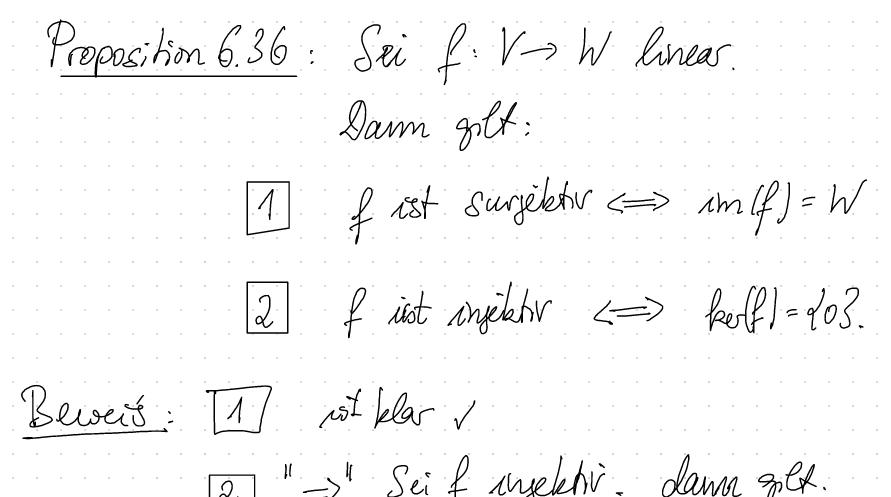
\includegraphics[width=10cm]{./_img/Istklar.jpeg}
        \centering \caption{Beispiel aus der LA1 vom Wintersemester 2020/21 für einen „Beweis“, in dem gar nichts argumentiert wurde. Vgl. die Begründung von \cref{def:surjektiv}.}
    \end{figure}
\end{bem}


\begin{bem}[Subjektivität des Beweisbegriffs]
    Das Wort „überzeugt“ in meiner Beweisdefinition deutet eine subjektive Komponente an. Wenn dich ein Vorlesungs-„Beweis“ nicht überzeugen kann, dann ist er für dich eben auch kein Beweis. Ein Beweistext kann für den Einen eine befriedigende Begründung sein, während er für den Anderen völlig unverständlich und praktisch wertlos ist. Wenn dir unmittelbar klar ist, dass eine Aussage gilt, kann sogar ein „Ist-klar-Beweis“ überzeugend sein.
    
    Nichtsdestotrotz gibt es gewisse Regeln und Techniken, über deren Zulässigkeit ein Konsens besteht. Beweise, die diesen Regeln unterliegen, muss ein Mathematiker anerkennen. Dass Beweise nicht überzeugend sind, kommt so gut wie nie von Verstößen gegen die Logik her; sondern eher von der Verwendung obskurer Begriffe, dem Mangel an Erläuterung komplizierter Beweisschritte, Schreibfehlern, dem Verschleiern von Beweislücken oder oder der unbegründeten Verwendung von Aussagen, die irgendwo fünfzig Seiten vorher einmal in einem unscheinbaren Lemma hergeleitet wurden.
\end{bem}


Bereits in diesem Kapitel werde ich Beweise führen, nämlich um zu demonstrieren, wie sich gewisse logische Schlussregeln und Beweistechniken aus anderen ableiten lassen. Setz dich aber nicht unter Druck, die Herleitungen der Beweistechniken lückenlos nachvollziehen zu müssen, sondern begreife sie als Erklärungen, die plausibel machen sollen, warum die Beweistechniken Sinn ergeben. Letztendlich musst du dich selbst davon überzeugen, wie genau ist gar nicht so wichtig. In den Mathevorlesungen (mal abgesehen von Vorlesungen über Logik, wo es genau darum geht) werden die üblichen Beweistechniken größtenteils ohne weitere Begründung verwendet und ab der zweiten Semesterwoche erwartet auch niemand mehr, dass du die Logik, die deinen Beweisen zugrundeliegt, rechtfertigst (solange sie halt nicht „unlogisch“ ist).





\section{Implikationen}


In diesem Abschnitt seien $A,B$ stets zwei beliebige Aussagen.


\begin{axiom}[Der direkte Beweis] \label{direkterbeweis} \index{Direkter Beweis}
    Um die Aussage „$A\to B$“ zu beweisen, kannst du die Technik des \textbf{direkten Beweises} benutzen:
    
    Nimmt an, dass die Aussage $A$ gilt und zeige nun mithilfe dieser Annahme (und aller weiteren Aussagen, die dir zur Verfügung stehen), dass auch $B$ gilt.
\end{axiom}


\begin{bsp}
    Sofern der FC Bayern München nach dem vorletzten Spieltag bereits vier Punkte vor dem Tabellenzweiten steht, wird er Deutscher Meister.
\end{bsp}


\begin{bew}
    Es sei einmal angenommen, der FC Bayern liege nach dem vorletzten Spieltag vier Punkte vor dem Tabellenzweiten. Weil nur noch ein Spieltag verbleibt, kann der Zweite (und jeder weiter unten stehende Verein) nur noch höchstens drei Punkte im letzten Spieltag gewinnen. Also sind dann die Bayern (schon wieder) uneinholbar und werden Deutscher Meister. \qed
\end{bew}


\begin{bem}[* Zusammenhang zur Interpretation von „$\to$“]
    In \cref{tauto} wurde die folgende Aussage T gezeigt:
    \begin{quote}
        (T): Die Implikation $A\to B$ ist genau dann eine Tautologie, wenn unter jeder (zweiwertigen) Interpretation, unter der $A$ eine wahre Aussage ist, auch $B$ eine wahre Aussage ist.
    \end{quote}
    Dies resultierte aus der Beschaffenheit der Wahrheitstafel für den Implikationspfeil:
    \[\begin{tabular}{cc|c}
        $A$ & $B$ & $A\to B$ \\
        \hline
        w & w & w \\
        w & f & f \\
        f & w & w \\
        f & f & w
    \end{tabular}\]
    Vermittels der Aussage (T) kann diese Wahrheitstafel zur Rechtfertigung der Technik des direkten Beweises verwendet werden. Umgekehrt kannst du aber auch die Technik des direkten Beweises als „natürlicher“ ansehen und die Aussage (T) als Rechtfertigung für die Wahrheitstafel des Implikationspfeils verstehen.
\end{bem}
  
  
\begin{bem}[Signalwörter]
    Wenn du die Implikation $A\to B$ direkt beweist, kannst du dies deutlich machen, indem du den Beweis mit „Es gelte $A$“, „Es sei angenommen, dass $A$ gilt“ oder Ähnlichem beginnst.
\end{bem}

  
\begin{satz}[* Jede Aussage impliziert sich selbst] \label{implikationref}
    Es gilt\footnote{vgl. \cref{teilmengeneig}a)}
    \[ A\to A \]
\end{satz}


\begin{bew}
    Für einen direkten Beweis sei angenommen, dass $A$ gilt. Weil unter dieser Annahme ja $A$ gilt, ist schon alles bewiesen. \qed
\end{bew}

  
\begin{satz}[* Wahres folgt aus Beliebigem]\label{wahresausbeliebigem}
    Es gilt
        \[ A \to (B\to A)   \]
    Mit anderen Worten: Sofern $A$ gilt, wird $A$ auch von $B$ impliziert.
\end{satz}


\begin{bew}
    Für einen direkten Beweis sei angenommen, dass $A$ gilt. Nun ist zu zeigen, dass auch $B\to A$ gilt. Dazu sei zusätzlich angenommen, dass $B$ gilt. Nun gilt auch $A$, weil dies ja schon ganz zu Beginn des Beweises angenommen wurde. \qed
\end{bew}


\begin{bem}[„$\to$“ bedeutet keine Kausalität!]
    Die Aussage, dass Wahres aus Beliebigem folgt, mag seltsam erscheinen (und wird unter die \href{https://de.wikipedia.org/wiki/Paradoxien_der_materialen_Implikation}{Paradoxien der materialen Implikation} gezählt), da dann ja auch Wahres aus solchen Aussagen folgt, die gar nichts damit zu tun haben. Beispielsweise ist „Sofern der Döner in Deutschland erfunden wurde, ist $4$ eine Quadratzahl“ eine wahre Aussage. Dass dies „paradox“ erscheint, kommt von einer inadäquaten Interpretation des Implikationspfeils „$\to$“:
    
    In ihrer üblichsten Interpretation besagt die Aussage $A\to B$ nicht, dass es einen kausalen Zusammenhang zwischen $A$ und $B$ geben muss; sondern nur, dass $B$ unter Annahme von $A$ gilt, egal ob diese Annahme in die Herleitung von $B$ mit einfließt oder nicht. Noch ein Beispiel: Da es, sofern sich das Rad einer Windmühle dreht, windig ist, ist „Wenn sich das Windrad dreht, ist es windig“ eine korrekte Aussage. Aber dies besagt natürlich nicht, dass es windig ist, \emph{weil} sich das Windrad dreht, geschweige denn, dass die Windmühle den Wind erzeugen würde.
\end{bem}


\begin{vorschau}[* Relevanzlogiken]
    Logiken, die sich darum bemühen, dass „$\to$“ wirklich die Bedeutung einer kausalen Implikation trägt, heißen „Relevanzlogiken“, da dort für eine Implikation $A\to B$ gefordert wird, dass $A$ in irgendeiner Hinsicht „relevant“ für $B$ ist. In Relevanzlogiken ist die Technik des direkten Beweises nicht mehr uneingeschränkt zulässig.
\end{vorschau}


\begin{axiom}[Modus ponens] \label{modusponens} \index{Modus Ponens}
    Die logische Schlussregel
    \[\begin{tabular}{r}
        $A\to B$ \\
        $A$ \\
        \hline
        $B$
   \end{tabular}\]
    heißt „Modus ponens“. Sie besagt: Wann immer dir gegeben ist, dass sowohl $A\to B$ als auch $A$ gültig sind, kannst du daraus $B$ schlussfolgern.
\end{axiom}


\begin{bsp}
    Ich habe angekündigt, dass ich, sofern ich zum Bürgermeister gewählt werde, Freibier für alle stiften werde. Sofern ich nun tatsächlich zum Bürgermeister gewählt werde, folgt, dass jedem Freibier ausgeschenkt wird.
\end{bsp}


\begin{bem}[Logik-Latein]
    Du brauchst dir nicht merken, dass diese Schlussregel „Modus ponens“ heißt. Ebensowenig brauchst du dir die anderen lateinischen Bezeichnungen in diesem Vortrag zu merken. Ich gebe die Wörter nur an, um dir das Nachschlagen in Internet und Literatur zu erleichtern.
\end{bem}


\begin{bem}
    \textbf{Vorsicht}: Anfänger machen gelegentlich den Fehler, aus $A\to B$ und $B$ auf die Aussage $A$ zu schließen. Hier ist ein Beispiel für diesen Fehlschluss:
    \begin{quote}
        Sei $x$ eine reelle Zahl. Bekanntlich gilt $(x=3)\to (x^2=9)$. Wenn also tatsächlich $x^2=9$ ist, so muss $x=3$ sein.
    \end{quote}
    Mach dir klar, warum diese Argumentation unzulässig ist.
\end{bem}


\begin{satz}[Direkter Beweis mit Zwischenschritten] \label{implikationtrans}
    Seien $n$ eine natürliche Zahl und $Z_1,\dots , Z_n$ eine Handvoll Aussagen. Um die Implikation $A\to B$ zu beweisen, kannst du die Implikationen
        \[ A\to Z_1,\quad Z_1\to Z_2,\quad \dots ,\quad Z_{n-1}\to Z_n\quad \text{und}\quad Z_n\to B \]
    beweisen.\footnote{vgl. \cref{teilmengeneig}b)} In diesem Fall verwendest du die Aussagen $Z_1,\dots , Z_n$ als \textbf{Zwischenschritte}.
\end{satz}


\begin{bew}
    Es sei angenommen, dass ich alle Implikationen $A\to Z_1$, $Z_1\to Z_2$, \dots , $Z_n\to B$ bewiesen habe. Um zu zeigen, dass dann auch $A\to B$ gilt, sei angenommen, dass $A$ gilt. Wegen $A\to Z_1$ folgt, dass dann auch $Z_1$ gilt. Wegen $Z_1\to Z_2$ folgt, dass auch $Z_2$ gilt. Auf diese Weise können wir schrittweise die $Z$'s durchgehen, sodass am Ende auch $Z_n$ bewiesen ist. Und wegen $Z_n\to B$ gilt dann auch $B$. \qed
\end{bew}


\begin{bsp}
    Falls es nächsten Sommer (schon wieder) zu wenig regnet, wird der Fichtenwald in meiner Heimatstadt gerodet werden.
\end{bsp}


\begin{bew}
    Wenn es nächstes Jahr wieder zu wenig regnet, fehlt es den Fichten an Flüssigkeit, um ausreichend Harz für eine widerstandsfähige Rinde auszubilden. Dies erleichtert es Borkenkäfern, innerhalb der Rinde zu nisten, sodass sich die Borkenkäferpopulation im Wald stark vergrößert und Bäume teilweise absterben werden. Unter diesem Umstand wird die örtliche Forstbehörde beschließen, den Wald zum Schutz vor umstürzenden Bäumen und einer weiteren Ausbreitung der Borkenkäfer zu roden. \qed
\end{bew}

  
\begin{nota}[*]
    Sind $n$ eine natürliche Zahl und $Z_1,\dots , Z_n$ ein paar Aussagen, für die $Z_1\to Z_2, Z_2\to Z_3, \dots, Z_{n-1}\to Z_n$ gilt, so schreibt man auch kurz
        \[ Z_1\to Z_2\to\ \dots\ \to Z_n\]
    Beispielsweise könnte die Argumentation von gerade eben folgendermaßen dargestellt werden:
    \begin{itemize}
        \item[] Nächstes Jahr regnet es zu wenig.
        \item[$\to$] Den Fichten fehlt es an Flüssigkeit, um ausreichend Harz für eine widerstandsfähige Rinde auszubilden.
        \item[$\to$] Borkenkäfern wird es erleichtert, innerhalb der Rinde zu nisten.
        \item[$\to$] Die Borkenkäferpopulation im Wald wird stark vergrößert und Bäume sterben teilweise ab.
        \item[$\to$] Die örtliche Forstbehörde beschließt, den Wald zum Schutz vor umstürzenden Bäumen und einer weiteren Ausbreitung der Borkenkäfer zu roden.   
    \end{itemize}
\end{nota}





\section{Äquivalenzen}


In diesem Abschnitt seien $A,B$ stets zwei beliebige Aussagen.


\begin{axiom}[Hin- und Rückrichtung] \label{hinruck} \index{Hinrichtung} \index{Rückrichtung} \index{Äquivalenzbeweis}
    Aus dem Vorliegen der beiden Implikationen $A\to B$ und $B\to A$ kann auf die Äquivalenz $A\leftrightarrow B$ geschlossen werden.\footnote{vgl. \cref{teilmengeneig}c)}
    \[\begin{tabular}{r}
        $A\to B$ \\
        $B\to A$ \\
        \hline
        $A\leftrightarrow B$
    \end{tabular}\]
    Wenn du die Äquivalenz $A\leftrightarrow B$ beweisen willst, kannst du deinen Beweis also in zwei Teile aufteilen: In der sogenannten \textbf{Hinrichtung} beweist du die Implikation $A\to B$. In der \textbf{Rückrichtung} beweist du die Implikation $B\to A$.
\end{axiom}


\begin{bsp} \label{bsp:hinruck}
    Sei $n$ eine ganze Zahl. Genau dann ist $n$ ein Vielfaches von $6$, wenn es zugleich ein Vielfaches von $2$ und ein Vielfaches von $3$ ist.
\end{bsp}


\begin{bew}
    \begin{enumerate}
        \item[„$\Rightarrow$“:] Sei $n$ ein Vielfaches von $6$. Dies besagt, dass es eine ganze Zahl $k$ mit $n=6\cdot k$ gibt. Es folgt
        \begin{align*}
            n= 2\cdot (3k) \qquad\text{und}\qquad n = 3\cdot (2k)
        \end{align*}
        also ist $n$ sowohl ein Vielfaches von $2$ als auch von $3$.
        \item[„$\Leftarrow$“:] Es sei $n$ sowohl ein Vielfaches von $2$ als auch von $3$. Demzufolge gibt es ganze Zahlen $k,l$ mit
        \begin{align*}
            n = 2k\qquad \text{und}\qquad n  = 3l
        \end{align*}
        Es folgt
        \begin{align*}
            n & = 1\cdot n \\
            & = (3-2)\cdot n \\
            & = 3n - 2n \\
            & = 3\cdot 2k - 2\cdot 3l & (\text{wegen $n=2k$ und $n=3l$})\\
            & = 6k - 6l \\
            & = 6\cdot (k-l)
        \end{align*}
        Also ist $n$ auch ein Vielfaches von $6$. \qed
    \end{enumerate}
\end{bew}


\begin{bem}
    Die Methoden, die in diesen Beweis eingingen, gehören zur „Teilbarkeitstheorie“. Mehr darüber wirst du im zweiten Semester in der Vorlesung „Lineare Algebra 2“ lernen.
\end{bem}


\begin{bem}[Signalwörter]
    Wenn du eine Äquivalenz per Hin- und Rückrichtung beweist, solltest du die jeweiligen Beweisteile mit „$\Rightarrow$“ und „$\Leftarrow$“ beginnen (so wie im Beispiel gerade eben) oder so etwas wie „Ich beweise zuerst die Hinrichtung“ und „Für den Beweis der Rückrichtung sei nun\dots“ schreiben, damit deinem Leser jederzeit klar ist, um welche der beiden Richtungen es gerade geht.
\end{bem}


\begin{axiom}
    Aus der Äquivalenz $A\leftrightarrow B$ kann sowohl auf $A\to B$ als auch auf $B\to A$ geschlossen werden.
    \[\begin{tabular}{r}
        $A\leftrightarrow B$ \\
        \hline 
        $A\to B$ 
    \end{tabular} \qquad\text{und}\qquad \begin{tabular}{r}
        $A\leftrightarrow B$ \\
        \hline 
        $B\to A$ 
    \end{tabular}\]
\end{axiom}


\begin{bsp}
    Es wurde angekündigt, dass man die Prüfung genau dann besteht, wenn man mehr als 50 Punkte erreicht hat. Dann weiß ich einerseits, dass, wenn ich die Prüfung bestanden habe, ich mehr als 50 Punkte erreicht haben muss; andererseits weiß ich, dass ich, sofern ich mindestens 50 Punkte erreicht habe, auf jeden Fall bestanden habe.
\end{bsp}


\begin{satz}[Äquivalenzbeweis mit Zwischenschritten] \label{ifftrans}
    Seien $n$ eine natürliche Zahl und $Z_1,\dots , Z_n$ ein paar Aussagen. Dann kannst du die Äquivalenz $A\leftrightarrow B$ beweisen, indem du die Äquivalenzen
        \[ A\leftrightarrow Z_1,\quad Z_1\leftrightarrow Z_2,\quad \dots,\quad Z_{n-1}\leftrightarrow Z_n \quad\text{und}\quad Z_n\leftrightarrow B \]
    beweist. In diesem Fall agieren die Aussagen $Z_1,\dots , Z_n$ in deinem Beweis als \textbf{Zwischenschritte}.
\end{satz}


\begin{bew}[*]
    \begin{enumerate}
        \item[„$\Rightarrow$“:] Aus den Äquivalenzen $A\leftrightarrow Z_1$, $Z_1\leftrightarrow Z_2$, \dots, $Z_n\leftrightarrow B$ folgen die Implikationen $A\to Z_1$, $Z_1\to Z_2$, \dots, $Z_n\to B$, woraus sich mittels \cref{implikationtrans} ergibt, dass $A\to B$ gilt.
        \item[„$\Leftarrow$“:] Aus den Äquivalenzen $A\leftrightarrow Z_1$, $Z_1\leftrightarrow Z_2$, \dots, $Z_n\leftrightarrow B$ folgen auch die Implikationen $B\to Z_n$, $Z_n\to Z_{n-1}$, \dots, $Z_1\to A$, woraus sich mittels \cref{implikationtrans} auch $B\to A$ ergibt. \qed
    \end{enumerate}
\end{bew}


\begin{nota}
    Sind $n$ eine natürliche Zahl und $Z_1,\dots , Z_n$ ein paar Aussagen, für die $Z_1\leftrightarrow Z_2,\dots, Z_{n-1}\leftrightarrow Z_n$ gilt, so schreibt man auch kurz
    \[ Z_1\leftrightarrow Z_2 \leftrightarrow \ldots \leftrightarrow  Z_n\]
\end{nota}


\begin{bsp}
    Sei $x$ eine positive reelle Zahl. Genau dann ist $x$ eine Lösung der Gleichung $x^2-x=1$, wenn $x= \frac{1+\sqrt{5}}{2}$.\footnote{Die Zahl $\frac{1+\sqrt{5}}{2}$ heißt \href{https://de.wikipedia.org/wiki/Goldener_Schnitt}{Goldener Schnitt}.}
\end{bsp}


\begin{bew}
    Es gilt:
    \begin{alignat*}{3}
        x^2-x& =1 \quad&\leftrightarrow\quad&& \left(x-\frac{1}{2}\right)^2 - \frac{1}{4} &= 1 \\
        && \leftrightarrow\quad&& \left(x-\frac{1}{2}\right)^2&=\frac{5}{4} \\
        && \leftrightarrow\quad&& x-\frac{1}{2} &= \pm \sqrt{\frac{5}{4}} \\
        && \leftrightarrow\quad&& x  &= \frac{1\pm \sqrt{5}}{2} 
    \end{alignat*}
    Weil $x$ positiv ist und $\frac{1-\sqrt{5}}{2}<0$ wäre, ist dies wiederum äquivalent zu $x=\frac{1+\sqrt{5}}{2}$. \qed
\end{bew}


\begin{satz}[* Jede Aussage ist äquivalent zu sich selbst]\label{iffref}
    Es gilt
        \[ A\leftrightarrow A \]
\end{satz}


\begin{bew}
    Mit \cref{implikationref} ist zugleich die Hinrichtung und die Rückrichtung bewiesen. \qed
\end{bew}


\begin{satz}[* Kommutativgesetz für $\leftrightarrow$]\label{iffkomm}
    Es gilt
        \[ (A\leftrightarrow B)\leftrightarrow(B\leftrightarrow A) \]
\end{satz}


\begin{bew}
    \begin{enumerate}
        \item[„$\Rightarrow$“:] Es gelte $A\leftrightarrow B$. Daraus folgt, dass sowohl $A\to B$ als auch $B\to A$ gelten. Das kann natürlich auch andersrum gelesen werden: es gelten sowohl $B\to A$ als auch $A\to B$. Hieraus folgt $B\leftrightarrow A$.
        \item[„$\Leftarrow$“:] Die Rückrichtung beweist man ganz analog zur Hinrichtung, dabei müssen lediglich die Rollen von $A$ und $B$ vertauscht werden. \qed
    \end{enumerate}
\end{bew}


\begin{bem}[Substitutionsprinzip] \index{Substitutionsprinzip}
    Seien $A,B$ zwei äquivalente Aussagen. Dann kannst du in Beweisen die Aussagen $A$ und $B$ beliebig miteinander vertauschen. Möchtest du beispielsweise $A$ beweisen, kannst du genausogut $B$ beweisen. Oder ist dir eine Aussage der Gestalt $(A\land C)\to D$ gegeben, so kannst du genausogut auch mit der Aussage $(B\land C)\to D$ arbeiten.
    
    Aus diesem Grund sind Äquivalenzaussagen wertvoll und nützlich. Sie erlauben es, Aussagen von mehreren Blickwinkeln zu beleuchten und dadurch ein „tieferes“ Verständnis für sie zu gewinnen.
\end{bem}


\begin{satz}[* Curry-Paradoxon\footnote{\href{https://de.wikipedia.org/wiki/Haskell_Brooks_Curry}{Haskell Curry (1900-1982)}}] \label{curryparadox}
    Es gilt
        \[ (A\leftrightarrow (A\to B))\to B \]
    Mit anderen Worten: Ist $A$ bereits äquivalent dazu, dass $B$ von $A$ impliziert wird, so gilt $B$.
\end{satz}


\begin{bew}
    Für einen direkten Beweis sei angenommen, dass $A\leftrightarrow (A\to B)$ gilt. Nun ist zu beweisen, dass $B$ gilt.
    \begin{enumerate}[(1)]
        \item Es gilt $A\to B$, denn: Für einen direkten Beweis sei angenommen, dass $A$ gilt. Wegen $A\leftrightarrow (A\to B)$ gilt dann auch $A\to B$. Und weil $A$ als gültig angenommen wurde, folgt daraus, dass $B$ gilt.
        \item Es gilt $B$, denn: Nach Schritt (1) gilt $A\to B$. Wegen $A\leftrightarrow (A\to B)$ gilt dann auch $A$. Weil nach Schritt (1) auch $A\to B$ gilt, folgt nun, dass auch $B$ gilt. \qed
    \end{enumerate}
\end{bew}


\begin{bem}[* Selbstreferenzielle Aussagen]
    Das Curry-Paradoxon wird deshalb als „Paradoxon“ gehandelt, da es zumindest in der Umgangssprache ziemlich leicht ist, Aussagen $A$ zu konstruieren, für die $A\leftrightarrow (A\to B)$ gilt. Zum Beispiel seien
    \begin{itemize}[labelindent=1.5em, leftmargin=!, labelwidth=\widthof{$B:=$}]
        \item[$A:=$] „Wenn diese Aussage wahr ist, gewinne ich morgen im Lotto.“
        \item[$B:=$] „Morgen gewinne ich im Lotto.“
    \end{itemize}
    Dann gilt tatsächlich $A\leftrightarrow (A\to B)$, sodass aus \cref{curryparadox} folgt, dass ich morgen Millionär bin. Lotterien hassen diesen Trick.
    
    Damit sich mit diesem Trick nicht einfach \emph{jede} mathematische Aussage beweisen lassen kann, muss sichergestellt werden, dass sich die Selbstreferenzialität „Wenn \emph{diese Aussage} wahr ist, dann \dots“, die umgangssprachlich problemlos erzeugbar ist, nicht in formaler mathematischer Sprache nachbilden lässt.
\end{bem}





\subsection*{* Drei häufige Anfängerfehler im Umgang mit Äquivalenzumformungen}


\begin{bem}[„Gleichungs-U's“]
    Aus der Schule sind es manche Studienanfänger gewohnt, Gleichungen dadurch zu beweisen, dass sie sie sovielen Äquivalenzumformungen unterziehen, bis am Ende eine „offensichtliche“ Gleichung rauskommt. Hier ein Beispiel für diese Vorgehensweise:
    \begin{bsp}
    Seien $x,y$ zwei reelle Zahlen. Dann gilt:
        \[ x\cdot (y+1)-x = (x+1)\cdot y-y\]
    \end{bsp}
    \begin{bew}[(Mieser Beweis)]
        Es gilt:
        \begin{alignat*}{3}
            && x\cdot (y+1)-x& \quad=\quad (x+1)\cdot y-y \\
            &\leftrightarrow\qquad& xy + x  -x& \quad=\quad xy + y - y \\
            &\leftrightarrow\qquad& xy & \quad=\quad xy
        \end{alignat*}
    \end{bew}
    Diesen „Beweisstil“ solltest du dir auf keinen Fall aneignen bzw. so bald es geht abgewöhnen! Denn bei so einer Äquivalenzenkette geschieht bei jeder Äquivalenzumformung auf jeder der beiden Seiten eine arithmetische Umformung, die der Leser nachvollziehen muss. Und diese arithmetischen Umformungen bilden den eigentlichen Kern des Beweises, letztendlich hat der Leser die Gleichungskette also in einer „U-Form“, deren beide Stränge erst ganz am Schluss zusammenfinden, zu lesen:
    \[\begin{tikzcd}
        && x\cdot (y+1)-x\ar[red, d, dash] & =& (x+1)\cdot y-y \ar[red, d, dash] \\
        &\leftrightarrow& xy + x-x  \ar[red, d, dash] & =& xy + y - y \ar[red, d, dash] \\
        &\leftrightarrow& xy \ar[red, rr, dash, bend right] & =& xy
    \end{tikzcd}\]
    Schöner ist, es diese Kette arithmetischer Umformungen, gar nicht erst als „U“, sondern als die Kette, als die sie letztendlich auch zu lesen ist, hinzuschreiben:
    \begin{bew}[(Schönerer Beweis)]
        Es gilt:
        \begin{align*}
            x\cdot (y+1) -x& = xy + x -x\\
            & = xy  \\
            & = xy + y - y \\
            & = (x+1)\cdot y -y  &&& \qed
        \end{align*}
    \end{bew}
    Unterscheide dabei sorgfältig von der Art und Weise, wie du den Beweis \emph{findest} und der Art und Weise, wie du ihn am Ende \emph{aufschreibst}\footnote{vgl \cref{rumprobieren} und \cref{beweisaufschreiben}}: Während des Beweisfindungsprozesses ist alles erlaubt und du darfst auf dem Schmierblatt soviele Äquivalenzumformungen aufschreiben, wie du willst. Aber am Ende, wenn es darum geht, den Beweis ansprechend aufzuschreiben, solltest du alle Unsauberkeiten tilgen und den Beweis in eine gut lesbare Form bringen. Ein mathematischer Beweis, wie du ihn in einem Lehrbuch findest oder wie ihn ein Dozent in der Vorlesung vorführt, gibt nur selten den Denkprozess, der seiner Entstehung zugrundelag, wieder. (Was in didaktischer Hinsicht manchmal bedauerlich und einer der Hauptgründe dafür ist, dass sich Erstsemester mit dem Verfassen von Beweisen schwertun.)
\end{bem}


\begin{bem}[Unterschied zwischen $=$ und $\leftrightarrow$]
    Bringe nicht $=$ und $\leftrightarrow$ durcheinander. Die Gleichheit „$=$“ ist eine Beziehung, die zwischen beliebigen Objekten desselben Typs Sinn ergibt. Bspw. ergibt es Sinn zu fragen, ob zwei Zahlen gleich sind, zwei Punkte im Raum gleich sind, zwei Funktionen dieselbe Ableitung haben usw. Dagegen ist „$\leftrightarrow$“ eine Beziehung zwischen \emph{Aussagen}. Manche sind es aus der Schule gewohnt, jegliche Art mathematischen Folgerns durch ein Gleichheitszeichen zu notieren. Die (korrekte) Gleichungsumformung
    \begin{align*}
        x & = y-3 \\
        \leftrightarrow\quad  x+3 & = y
    \end{align*}
    würden sie inkorrekterweise als
    \begin{align*}
        x & = y-3 \\
        = \quad x+3 & = y
    \end{align*}
    notieren, was Leser arg verwirren kann (vor allem, wenn es nicht so schön eingerückt wäre, sondern einfach nur $x=y-3=x+3=y$ dastünde) und auch schlicht mathematisch falsch ist.
    
    Auch hier gilt wieder: In der kreativen Phase, in der du nach einem Beweis suchst und Schmierblatt um Schmierblatt mit Ideen vollschreibst, darfst du Gleichheitszeichen nach Belieben spammen und sogar falsch verwenden. Aber bei der Erstellung des Endprodukts, des Beweises, wie ihn Andere lesen sollen, solltest du penibel auf die korrekte Verwendung von „$=$“'s und „$\leftrightarrow$“'s achten.
\end{bem}


\begin{bem}[Beweise „rückwärts“ führen] \label{hintennachvorne}
    Mal angenommen, ich möchte beweisen, dass die Kubikwurzel von $3$ größer als die Quadratwurzel von $2$ ist. Auf der Suche nach einem Beweis beginne ich einfach mal mit der zu zeigenden Ungleichung $\sqrt[3]{3}>\sqrt{2}$ und forme ein bisschen um:
    \begin{align*}
        && \sqrt[3]{3}& >\sqrt{2} \\
        & \to& \sqrt[3]{3}^{3\cdot 2} & > \sqrt{2}^{2\cdot 3} & (\text{beide Seiten mit $6$ potenzieren}) \\
        & \to & (\sqrt[3]{3}^3)^2 & > (\sqrt{2}^2)^3 & (\text{Potenzgesetz anwenden})\\
        & \to & 3^2 & > 2^3 \\
        & \to & 9 & > 8
    \end{align*}
    Das sieht schonmal gut aus! Durch ein paar Umformungen bin ich auf eine wahre Aussage gelangt. Mancher Anfänger würde nun denken, dass das Problem damit erledigt ist und die obige Ungleichungskette als Beweis taugt.
    
    Das ist aber falsch. Denn die Ungleichungskette beginnt ja mit der zu beweisenden Aussage. Hier wurde also nur die Aussage „Wenn $\sqrt[3]{3} >\sqrt{2}$ gilt, dann ist $9>8$“ bewiesen, die aber leider nichts darüber aussagt, ob nun tatsächlich $\sqrt[3]{3} >\sqrt{2}$ gilt. Glücklicherweise handelt es sich bei allen Umformungen sogar um Äquivalenzumformungen, sodass die Ungleichungskette auch in umgekehrter Richtung gültig ist:
    \begin{align*}
        && 9 & > 8 \\
        & \to & 3^2 & > 2^3 \\
        & \to & (\sqrt[3]{3}^3)^2 & > (\sqrt{2}^2)^3 \\
        & \to& \sqrt[3]{3}^{3\cdot 2} & > \sqrt{2}^{2\cdot 3} & (\text{Potenzgesetz anwenden}) \\
        &\to &  \sqrt[3]{3}& >\sqrt{2}  & (\text{sechste Wurzel ziehen})
    \end{align*}
    Nun ist die Argumentation zumindest mal nicht mehr mathematisch falsch. Wenn ich jetzt noch das „Ungleichungs-U“ loswerde, kann sich der Beweis sehen lassen. Hier ist der finale Beweis:
    \begin{bew}
        Es gilt
        \begingroup
        \allowdisplaybreaks
        \begin{align*}
            \sqrt[3]{3} & = \sqrt[3]{\sqrt{9}} \\
            & = \sqrt[6]{9} \\
            & > \sqrt[6]{8} & (\text{da $\sqrt[6]{-}$ eine ordnungserhaltende Operation und $9>8$ ist}) \\
            & = \sqrt{\sqrt[3]{8}} \\
            & = \sqrt{2} && \qed
        \end{align*}
        \endgroup
    \end{bew}
    Beachte, dass die Struktur dieses Beweises nicht meinen Denkprozess bei der Beweissuche wiederspiegelt. Das ist aber völlig normal und ok. Sollte dein Beweis sehr kompliziert sein, wäre es natürlich trotzdem nett, wenn du, sofern es deinem Leser hilft, ein paar Meta-Bemerkungen darüber, welche Idee hinter dem aktuellen Beweisschritt steckt, einstreust.
    
    Auch Profis stoßen manchmal auf einen Beweis, indem sie die Argumentation „rückwärts“ ausprobieren, also mit der zu beweisenden Aussage starten und schauen, was sich damit anfangen lässt. Während diese Strategie völlig legitim zur Beweis\emph{findung} ist, ist sie es aber nicht zur Beweis\emph{niederschrift}. Dein zum Schluss aufgeschriebener Beweis muss das Problem sauber von den gegebenen Aussagen auf die zu beweisenden Aussagen durchgehen.
    
    Der Versuch, einen Beweis rückwärts zu führen, kann auch Fehler erzeugen, die du, sofern du den Rückwärts-Gedankengang am Ende nicht kritisch reflektierst, übersiehst. Zum Beispiel könnte man meinen, dass für jede reelle Zahl $x$ gilt, dass $\cos(x)=\sqrt{1-\sin^2(x)}$. Denn man kann ja umformen
    \begin{align*}
        &&\cos(x)& =\sqrt{1-\sin^2(x)} \\
        & \to & \cos^2(x)& = 1-\sin^2(x) & (\text{beide Seiten quadrieren}) \\
        & \to & \cos^2(x) + \sin^2(x) &= 1
    \end{align*}
    und letzteres ist eine wohlbekannte wahre Aussage (die manchmal als „Satz des Pythagoras“ bezeichnet wird). Jedoch ist
        \[ \cos(\pi) = -1 \neq 1 = \sqrt{1-0^2} = \sqrt{1-\sin^2(\pi)} \]
    sodass irgendetwas nicht stimmen kann. Kannst du ausmachen, wie und wo genau sich der Fehler eingeschlichen hat?
\end{bem}


\begin{bem}[Weitere Anfängerfehler]
 Eine lange Liste von sowohl studentischen als auch dozentischen Fehlern, die ihm während seiner Lehrtätigkeit aufgefallen sind, hat Eric Schechter auf \href{https://math.vanderbilt.edu/schectex/commerrs/}{seiner Homepage} zusammengetragen.
\end{bem}





\subsection*{* Mehrfach-Äquivalenzen}


\begin{de}[„Die folgenden Aussagen sind äquivalent“] \label{def:tfae}
    Einige mathematische Sätze haben die Gestalt einer größeren Äquivalenzaussage und sehen etwa folgendermaßen aus:
    \begin{quote}
        Es seien \dots und es gelte \dots. Dann sind die folgenden Aussagen äquivalent:
        \begin{itemize}
            \item[(i)] \dots
            \item[(ii)] \dots
            \item[(iii)] \dots
            \item[(iv)] \dots
            \item[\dots]
        \end{itemize}
    \end{quote}
    Diese Satzstruktur kommt so häufig vor, dass sie im Englischen durch ``tfae'' abgekürzt wird (für ``the following are equivalent''). Sie besagt, dass je zwei der Aussagen (i), (ii), (iii), usw. zueinander äquivalent sind, also dass alle Äquivalenzen
        \[ \text{(i)$\leftrightarrow$(ii),\quad (i)$\leftrightarrow$(iii), \quad (ii)$\leftrightarrow$(iii),\quad (i)$\leftrightarrow$(iv),\quad (ii)$\leftrightarrow$(iv), \quad (iii)$\leftrightarrow$(iv),\quad \dots} \]
    gelten. Man sagt auch, die Aussagen seien „paarweise äquivalent“.
 \end{de}
 
 
\begin{bsp}
    Sei $D$ ein Dreieck in der euklidischen Ebene. Dann sind die folgenden Aussagen äquivalent:
    \begin{enumerate}[(i)]
        \item $D$ ist ein gleichseitiges Dreieck, d.h. alle Seiten von $D$ haben dieselbe Länge.
        \item Alle Innenwinkel von $D$ haben dieselbe Größe.
        \item Der Schwerpunkt von $D$ stimmt mit seinem Umkreismittelpunkt überein.
        \item Der Schwerpunkt von $D$ stimmt mit seinem Inkreismittelpunkt überein.
    \end{enumerate}
Würde man hier die Äquivalenz jedes Aussagenpaars per Hin- und Rückrichtung beweisen, müsste man insgesamt zwölf Implikationen beweisen. Mit der folgenden Beweistechnik lässt sich in solchen Fällen erheblich Arbeit einsparen:
\end{bsp}


\begin{satz}[Ringschluss] \label{ringschluss} \index{Ringschluss}
    Seien $n$ eine natürliche Zahl und $A_1,\dots , A_n$ eine Handvoll Aussagen, von denen du beweisen möchtest, dass sie paarweise äquivalent sind. Dann kannst du dies mit der Technik des \textbf{Ringschlusses} erledigen, indem du lediglich die Implikationen
        \[ A_1\to A_2,\quad A_2\to A_3,\quad \dots ,\quad A_{n-1}\to A_n,\quad A_n\to A_1 \]
    beweist. Auf diese Weise „schließt du einen Ring“ zwischen den Aussagen $A_1,\dots , A_n$.
\end{satz}


\begin{bew}
    Durch den Ringschluss wurden alle Implikationen im folgenden Diagramm bewiesen:
    \[\begin{tikzcd}
        &&& A_1 \ar[rrd] &&& \\
        &A_n\ar[rru]&&&& A_2 \ar[ld]& \\
        && \dots \ar[lu] && A_3 \ar[ll]&& 
    \end{tikzcd} \]
    Man sieht, dass sich nun von jeder Aussage mittels Zwischenschritten zu jeder anderen Aussage gelangen lässt, solange man nur lang genug „im Uhrzeigersinn läuft“. Wegen \cref{implikationtrans} gilt daher für je zwei Aussagen $B,C$ aus den $A_1,\dots , A_n$, dass $B\to C$ und $C\to B$, also insgesamt $B\leftrightarrow C$. Demzufolge sind je zwei beliebige Aussagen aus $A_1,\dots , A_n$ zueinander äquivalent. \qed
\end{bew}


\begin{bsp} \label{bsp:ringschluss}
    Sei $n$ eine ganze Zahl. Dann sind die folgenden Aussagen äquivalent:
    \begin{enumerate}[(i)]
        \item Es ist $n\ge 1$.
        \item Für jede ganze Zahl $m$ ist $m+n>m$.
        \item Es gibt mindestens eine ganze Zahl $m$, für die $m+n>m$ gilt.
    \end{enumerate}
\end{bsp}


\begin{bew}
    (i)$\to$(ii): Es gelte (i) und es sei $m$ eine beliebige ganze Zahl. Dann ist
    \begin{align*}
        m+n & \ge m+1 && (\text{wegen (i)}) \\
        & > m
    \end{align*}
    (ii)$\to$(iii) ist trivial, da ganze Zahlen existieren. \\[0.5em]
    (iii)$\to$(i): Es gelte (iii). Dann gibt es eine ganze Zahl $m$ mit $m+n>m$. Subtraktion von $m$ liefert die Ungleichung $n>0$. Und da $n$ eine ganze Zahl ist, muss dann schon $n\ge 1$ gelten. \qed
\end{bew}


\begin{bem}
    \textbf{Achtung}: Ein gelegentlicher Anfängerirrtum besteht darin, zu denken, der Ringschluss müsse \emph{immer} in der Form (i)$\to$(ii), (ii)$\to$(iii), (iii)$\to$(i) durchgeführt werden. Das ist Unsinn und führt dazu, dass sich manche Anfänger einen Haufen unnötige Mehrarbeit aufhalsen.
    
    Genausogut kannst du etwa auch einen Ringschluss über die Implikationen (ii)$\to$(i), (iii)$\to$(ii) und (i)$\to$(iii) durchführen.
    
    Manchmal ist die Ringschluss-Methode auch unangebracht, wenn etwa die beiden Aussagen (ii) und (iii) so widerspenstig gegeneinander sind, dass keine Beweise für (ii)$\to$(iii) und (iii)$\to$(ii) in Sicht sind. In diesem Fall ist es vielleicht einfacher, den scheinbar längeren Weg zu gehen und (i)$\to$(ii), (ii)$\to$(i), (i)$\to$(iii) und (iii)$\to$(i) zu beweisen.
    \[\begin{tikzcd}[column sep=small]
        & (ii) \ar[rd] & \\
        (iii)\ar[ru] && (i)\ar[ll]
    \end{tikzcd}\qquad\text{anstelle von}\qquad\begin{tikzcd}[column sep=small]
        & (i) \ar[rd] & \\
        (iii)\ar[ru] && (ii)\ar[ll]    
    \end{tikzcd}\qquad\text{geht auch.}\]
    \[\text{Manchmal funktioniert aber nur}\qquad \begin{tikzcd}
        & (i) \ar[ld, bend right=20]  \ar[rd, bend right=20] & \\
        (iii)\ar[ru, bend right=20] && (ii) \ar[lu, bend right=20]
    \end{tikzcd}\]
    Entscheidend ist, dass du am Ende so viele Implikationen bewiesen hat, dass man mittels Zwischenschritten von jeder Aussage zu jeder anderen Aussage gelangen kann. \\[0.5em]
    Wenn du eine längere Äquivalenzaussage beweisen möchtest, solltest du immer Ausschau nach Implikationen halten, die „geschenkt“ sind, d.h. deren Beweis besonders naheliegend und einfach ist (in \cref{bsp:ringschluss} war das die Implikation (ii)$\to$(iii)). Daran kannst du dann deine Beweisstrategie orientieren. Ein berüchtigter Äquivalenzbeweis in der LA1-Vorlesung vom Wintersemester 2016/17 verlief so kompliziert, dass der Dozent zu Beginn seines Beweises einen „Plan“ aufgeschrieben hat, um den Studis die Orientierung zu erleichtern.
    \begin{figure}[ht]
        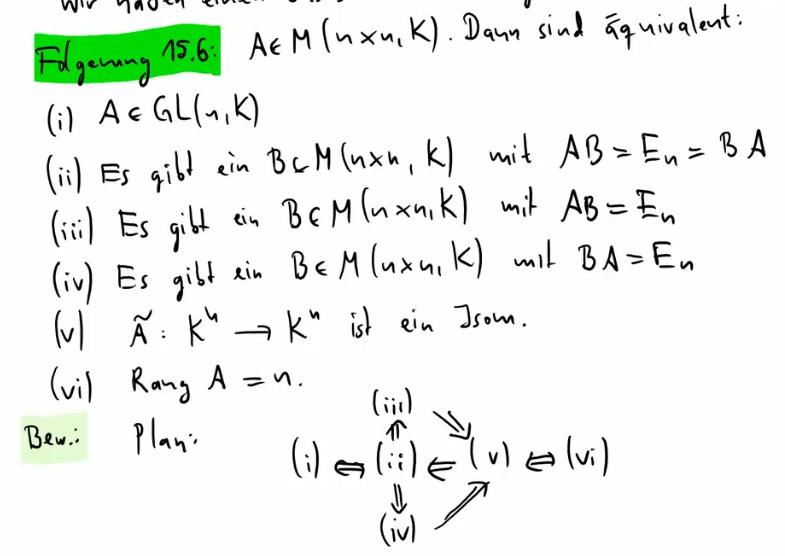
\includegraphics[width=10cm]{./_img/equivbeweis.jpeg}
        \centering \caption{Eine Äquivalenzaussage aus der LA1 vom WS16/17. Hier sind die Implikationen (ii)$\to$(iii) und (ii)$\to$(iv) „geschenkt“.}
    \end{figure}
\end{bem}


\begin{bem}[Signalwörter]
    Wenn du eine Aussage der Gestalt „Folgende Aussagen sind äquivalent\dots“ beweist, solltest du den Beweis jeder einzelnen Implikation mit „(i)$\to$(ii)“, „(iii)$\to$(i)“ oder Ähnlichem betiteln, damit deinem Leser jederzeit klar ist, welche Implikation gerade Thema ist.
\end{bem}





\section{Und und Oder}


In diesem Abschnitt seien $A,B$ stets zwei beliebige Aussagen


\begin{axiom}[*]\label{undoderaxiome}
    Für je zwei Aussagen $A,B$ gelten:
    \begin{align*}
        (A\land B) & \to A & A & \to (A\lor B) \\
        (A\land B) & \to B & B & \to (A\lor B)
    \end{align*}
    Mit anderen Worten: Aus $A\land B$ folgt sowohl $A$ als auch $B$; und $A$ und $B$ sind wiederum hinreichende Bedingungen für $A\lor B$.
\end{axiom}


\begin{bem}
    Wenn dir die Aussage $A\land B$ gegeben ist, kannst du das also so behandeln, als hättest du zwei gegebene Aussagen, nämlich $A$ und $B$.
    
    Und wenn du $A\lor B$ beweisen möchtest, würde es schon reichen, wenn du $A$ beweist oder wenn du $B$ beweist.
\end{bem}


\begin{axiom}[Und-Aussagen beweisen] \label{undbeweise}
    Um die Aussage $A\land B$ zu beweisen, genügt es, sowohl $A$ als auch $B$ zu beweisen:
    \[\begin{tabular}{r}
        $A$ \\
        $B$ \\
        \hline 
        $A\land B$
    \end{tabular} \]
    Mit anderen Worten: Wenn „$A\land B$“ auf deiner „zu zeigen“-Liste steht, kannst du das als zwei separate Ziele behandeln, nämlich musst du einerseits $A$ und andererseits $B$ beweisen.
\end{axiom}


\begin{bsp}[*]
    Die $25$ ist eine Quadratzahl, die sich als Summe zweier echt kleinerer Quadratzahlen schreiben lässt. Außerdem ist sie die kleinste Quadratzahl mit dieser Eigenschaft.
\end{bsp}


\begin{bew}
    (1) Aus
        \[ 25=5^2 \qquad\text{und}\qquad 25 = 9 + 16 = 3^2 + 4^2 \]
    folgt, dass $25$ eine Quadratzahl ist, die sich als Summe zweier echt kleinerer Quadratzahlen schreiben lässt.
    
    (2) Die einzigen Quadratzahlen $\neq 0$, die noch kleiner als $25$ sind, sind
        \[ 1\qquad 4\qquad 9\qquad 16 \]
    Wäre eine dieser vier Zahlen eine Summe zweier echt kleinerer Quadratzahlen, so müssten auch diese beiden Summanden in der Liste dieser vier Zahlen vorkommen. Aber alle möglichen Summationen
    \begin{align*}
        1+1 & = 2 & 1+4 & = 5 \\
        1+ 9 & = 10 & 1+16 & = 17 \\
        4 + 4 & = 8 & 4+9 & = 13 \\
        4+16 & = 20 & 9+9 & = 18
    \end{align*}
    ergeben keine Quadratzahl. \qed
\end{bew}


\begin{bem}[*]
    Drei natürliche Zahlen $a,b,c$, für die $a^2+b^2=c^2$ gilt, heißen ein \textbf{pythagoräisches Tripel}. Also wurde gerade bewiesen, dass $(2,3,5)$ das kleinste pythagoräische Tripel ist. Nach dem berühmten \href{https://de.wikipedia.org/wiki/Gro\%C3\%9Fer_Fermatscher_Satz}{Großen Satz von Fermat} besitzt die Gleichung $a^n+b^n=c^n$ für eine natürliche Zahl $n\ge 3$ keine positive ganzzahlige Lösung.
\end{bem}


\begin{axiom}[Beweis mit Fallunterscheidung] \label{fallunterscheidung} \index{Fallunterscheidung (in einem Beweis)}
    Sei $X$ eine Aussage, die du beweisen möchtest. Außerdem sei gegeben, dass $A\lor B$ gilt\footnote{Im Englischen sagt man: ``the two cases $A$ and $B$ are \emph{exhausting}''.}. Dann kannst du $X$ mittels einer \textbf{Fallunterscheidung} beweisen, indem du sowohl zeigst, dass $A\to X$ gilt, als auch, dass $B\to X$ gilt.
\end{axiom}


\begin{bsp} \label{bsp:fallunterscheidung}
    Für jede natürliche Zahl $n$ ist $n\cdot (n+1)$ eine gerade Zahl.
\end{bsp}


\begin{bew}
    Da jede natürliche Zahl entweder gerade oder ungerade ist, führe ich eine Fallunterscheidung durch:
    \begin{enumerate}[label={(Fall \arabic*):}, labelindent=1.5em, leftmargin=!, labelwidth=\widthof{(Fall 2):}]
        \item $n$ ist eine gerade Zahl. In diesem Fall ist $n\cdot (n+1)$ als Vielfaches der geraden Zahl $n$ ebenfalls eine gerade Zahl.
        \item $n$ ist eine ungerade Zahl. In diesem Fall ist $n+1$ eine gerade Zahl, sodass $n\cdot (n+1)$ als Vielfaches der Zahl $n+1$ ebenfalls eine gerade Zahl ist.
    \end{enumerate}
    Also ist $n\cdot(n+1)$ in jedem Fall gerade. \qed
\end{bew}





\section{Quantoren}


In diesem Abschnitt sei $E(x)$ stets ein einstelliges Prädikat.


\begin{axiom}[*] \label{quantorenaxiom}
    Sei $a$ irgendein Objekt. Dann gelten die folgenden beiden Implikationen:
    \begin{align*}
         \forall x: E(x) \quad& \to\quad E(a) \\
         E(a) \quad & \to\quad \exists x: E(x)
    \end{align*}
\end{axiom}

 
\begin{bsp}[*] \quad
    \begin{enumerate}
        \item Weil jede positive reelle Zahl eine Qudaratwurzel besitzt, existiert insbesondere auch eine reelle Quadratwurzel der Zwei.
        \item Es existieren $p,q,x,y\in \N_{\ge 1}$ mit $x^p-y^q=1$, denn $3^2-2^3=1$. (Nach dem \href{https://de.wikipedia.org/wiki/Catalansche_Vermutung}{Satz von Catalan-Mihăilescu} gibt es aber keine weiteren Möglichkeiten) 
    \end{enumerate}
\end{bsp}


\begin{satz}[Beweis per Beispiel] \label{beweisperbsp} \index{Beispiel (in einem Beweis)}
    Du kannst die Existenzaussage $\exists x: E(x)$ dadurch beweisen, dass du ein konkretes Objekt $a$ findest, das die Eigenschaft $E$ besitzt. Man nennt dann $a$ ein \textbf{Beispiel} für die Existenzaussage $\exists x: E(x)$.
\end{satz}


\begin{bew}
    Ergibt sich direkt aus der Formel $E(a)\to\exists x:E(x)$. \qed
\end{bew}


\begin{bsp}
    Es gibt eine natürliche Zahl $n\ge 1$, die gleich der Summe ihrer echten Teiler ist.\footnote{Zahlen, die gleich der Summe ihrer echten Teiler sind, heißen auch \href{https://de.wikipedia.org/wiki/Vollkommene_Zahl}{vollkommene Zahlen}.}
\end{bsp}


\begin{bew}
    Ein Beispiel ist die Zahl $28$. Denn die echten Teiler der $28$ sind genau
        \[ 1 \qquad 2 \qquad 4 \qquad 7 \qquad 14 \]
    und es $1+2+4+7+14=28$. \qed
\end{bew}

  
\begin{bem}
    Lässt sich eine Existenzaussage mit einem Beispiel beweisen, so ist es eigentlich schlechter Stil, in einem Buch oder einem Vortrag nur die Existenzaussage anzugeben. Beispielsweise ist ja die Information „Die $24$ ist gleich der Summe ihrer echten Teiler“ umfangreicher als die Information „Es gibt eine natürliche Zahl, die gleich der Summe ihrer echten Teiler ist“. Du solltest dir nicht einfach nur die Existenzaussage merken, sondern, sofern es welche gibt, auch ein paar Beispiele und deren Konstruktion im Hinterkopf behalten. Auch die essenzielle Aussage des Satzes von Euklid \cref{euklid} besteht weniger in der Aussage „Es gibt eine Primzahl, die größer als $n$ ist“ als vielmehr in der trickreichen Art und Weise, wie eine solche Primzahl aufgespürt wird.
    
    Es gibt allerdings auch Situationen, in denen eine Existenzaussage beweisbar ist, obwohl es unmöglich ist, konkrete Beispiele zu geben. Falls in einer Vorlesung keine Beispiele gegeben werden (was bedauerlicherweise recht häufig vorkommt und dem Zeitdruck im Vorlesungsbetrieb zu verdanken ist), solltest du beim Prof. nachhaken, ob er/sie vielleicht deshalb keine Beispiele bringt, weil es gar keine gibt oder die wenigen bekannten Beispiele zu kompliziert und zeitaufwendig sind. Gute Bücher und Vorlesungen erkennt man daran, dass sie, wenn sie keine Beispiele geben, auch erklären, warum.
\end{bem}


\begin{axiom}[Allaussagen an einem „beliebigen“ Objekt nachweisen]\label{allbeweis} \index{beliebig}
    Um die Allaussage $\forall x: E(x)$ zu beweisen, kannst du folgendermaßen vorgehen:
    
    Führe eine Variable $a$, die bislang noch nicht im Beweis verwendet wurde und ein \emph{beliebiges} Objekt bezeichnen soll, ein und beweise nun, dass $a$ die Eigenschaft $E$ besitzt.
\end{axiom}


\begin{bsp} \label{bsp:allbeweis}
    Für jede reelle Zahl $x\neq 1$ existiert eine reelle Zahl $y$ mit $x=\frac{y+1}{y-2}$.
\end{bsp}


\begin{bew}
    Sei $x$ eine beliebige reelle Zahl $\neq 1$. Wegen $x\neq 1$ ist $x-1\neq 0$, sodass durch $y:= \frac{1+2x}{x-1}$ eine wohldefinierte reelle Zahl gegeben ist. Nun rechnet man nach, dass $y\neq 2$ und $\frac{y+1}{y-2}=x$. \qed
\end{bew}

  
\begin{bem}[Signalwörter]
    Ein Beweis einer Allaussage beginnt meist mit Floskeln wie „Sei $x$ ein beliebiges\dots“ oder „Die Zahl $n$ sei beliebig aber fest“. Viele Texte lassen das Signalwort „beliebig“ auch weg und beginnen schlicht mit sowas wie „Sei $x$ eine reelle Zahl. Dann \dots“. Sie setzen vom Leser voraus, dass er erkennt, dass hier gerade der Beweis einer Allaussage beginnt.
\end{bem}
  
 
\begin{bem}[*]
    Achte darauf, dass die von dir eingeführte Variable, die das „beliebige“ Objekt bezeichnen soll, auch wirklich nirgendwo sonst im bisherigen Beweis aufgetaucht ist, also auch wirklich „beliebig“ ist. Ansonsten könnte dir ein Fehler wie der folgende passieren:
    \begin{bsp}[*]
        Es gibt eine natürliche Zahl $n$, die größergleich jede andere natürliche Zahl ist.
    \end{bsp}
    \begin{bew}
        Setze $n=0$. Es bleibt zu zeigen, dass jede natürliche Zahl kleinergleich $n$ ist. Dazu sei $n$ eine beliebige natürliche Zahl. Weil bekanntlich stets $n\le n$ gilt, ist also jede beliebige Zahl kleinergleich $n$.
    \end{bew}
        Ganz so offensichtliche Fehler passieren natürlich eher selten. Subtilere Fehler dieser Art kommen aber durchaus vor.
\end{bem}


\begin{bsp}[* Satz von Euklid] \label{euklid}
    Für jede natürliche Zahl $n$ gibt es eine Primzahl, die größer als $n$ ist.
\end{bsp}


\begin{bem}
    Die logische Struktur dieses Satzes ist
        \[ \forall\ (\text{natürliche Zahl $n$})\ \exists\ (\text{Primzahl $P$}):\ P>n \]
    Da es sich insgesamt um eine Allaussage handelt, sollte der Beweis mit „Sei $n$ eine beliebige natürliche Zahl“ beginnen. Da daraufhin die Existenzaussage
        \[ \exists P\in \N:\ \text{$P$ ist eine Primzahl und größer als $n$} \]
    übrig bleibt, fährt der Beweis nun mit der geschickten Konstruktion eines Beispiels fort:
\end{bem}


\begin{bew}
    Sei $n$ eine beliebige natürliche Zahl. Da es nur endlich viele natürliche Zahlen gibt, die $\le n$ sind, gibt es auch nur endlich viele Primzahlen, die $\le n$ sind. Seien $k$ deren Anzahl und $p_1,\dots , p_k$ diese Primzahlen. Betrachte die Zahl\footnote{Im Fall $k=0$ ist $N=2$, weil dann ein „leeres Produkt“ involviert ist, siehe \cref{mehrfachprodukt}.}
        \[ N := p_1\cdot\ldots\cdot p_k + 1 \]
    Dann lässt $N$ bei der Division durch $p_1,\dots , p_k$ jedes Mal den Rest Eins übrig, ist also nicht durch $p_1,\dots , p_k$ teilbar. Wegen $N\ge 2$ muss $N$ gemäß dem Fundamentalsatz der Arithmetik aber mindestens einen Primteiler $P$ besitzen. Da $P$ keines der $p_1,\dots ,p_k$ sein kann, aber die $p_1,\dots , p_k$ alle Primzahlen sind, die $\le n$ sind, muss $P$ größer als $n$ sein. \qed
\end{bew}


\begin{axiom}[* Verwenden von Existenzaussagen] \label{exverwendung}
    Sofern dir in einem Beweis eine Aussage der Gestalt $\exists x: E(x)$ gegeben ist, kannst du eine Variable $a$, die bisher noch nirgends im Beweis aufgetaucht ist, einführen, und die Aussage $E(a)$ als gegeben annehmen.
\end{axiom}
  
  
\begin{bsp} \label{bsp:exverwendung}
    Die Gleichung $x^5=x+1$ besitzt eine reelle Lösung.\footnote{vgl. \cref{zeichendefinieren}}
\end{bsp}


\begin{bew}
    Betrachte die reelle Funktion
        \[ f(x) = x^5-x-1 \]
    Dann gilt $f(1)=-1$ und $f(2)=29$. Somit folgt aus dem Zwischenwertsatz der Analysis, dass $f$ eine Nullstelle irgendwo zwischen $1$ und $2$ haben muss. Sei $\xi$ eine solche Nullstelle (hier wird \cref{exverwendung} genutzt). Dann gilt $\xi^5-\xi-1=0$, also $\xi^5=\xi +1$. \qed
\end{bew}


\begin{satz}[* Vertauschbarkeit von Quantoren derselben Sorte] \label{quantorentausch}
    Sei $R$ ein zweistelliges Prädikat. Dann gilt:
    \begin{align*}
        \forall x\ \forall y: R(x,y) \quad &\leftrightarrow\quad \forall y\ \forall x: R(x,y) \\
        \exists x\ \exists y: R(x,y) \quad &\leftrightarrow\quad  \exists y\ \exists x: R(x,y)
    \end{align*}
\end{satz}


\begin{bew}
    Ich beweise jeweils nur die Hinrichtung „$\to$“. Die Rückrichtung wird analog unter Vertauschung der Rollen von $x$ und $y$ bewiesen.
    \begin{itemize}
        \item[„$\forall$“:] Seien $a,b$ zwei beliebige Objekte und es gelte $\forall x\ \forall y: R(x,y)$. Mit \cref{quantorenaxiom} folgt durch Einsetzen von $a$, dass $\forall y: R(a,y)$ und durch Einsetzen von $b$, dass $R(a,b)$. Da $a$ beliebig gewählt war, gilt somit sogar $\forall x: R(x,b)$. Und da auch $b$ beliebig gewählt war, folgt hieraus, dass $\forall y\ \forall x: R(x,y)$.
        \item[„$\exists$“:] Es sei angenommen, dass $\exists x\ \exists y: R(x,y)$ gilt. Dann gibt es ein Objekt $a$, für das $\exists y: R(a,y)$ gilt. Damit gibt es auch ein Objekt $b$, für das $R(a,b)$ gilt. Wegen $R(a,b)$ gilt insbesondere $\exists x: R(x,b)$ und daraus folgt wiederum $\exists y\ \exists x: R(x,y)$. \qed
    \end{itemize}
\end{bew}


\begin{satz}[* Quantoren verschiedener Art sind nicht miteinander vertauschbar!]
    Sei $R$ ein zweistelliges Prädikat. Dann gilt zwar
        \[ \exists x\ \forall y: R(x,y) \quad\to\quad \forall y\ \exists x: R(x,y) \]  
    die umgekehrte Implikation „$\leftarrow$“ ist im Allgemeinen aber falsch, vgl. \cref{quantorreihenfolge}.
\end{satz}


\begin{bew}
    Sei $b$ ein beliebiges Objekt und es gelte $\exists x\ \forall y: R(x,y)$. Dann gibt es ein Objekt $a$, für das $\forall y: R(a,y)$ gilt. Also gilt insbesondere $R(a,b)$. Daraus folgt $\exists x: R(x,b)$ und da das Objekt $b$ beliebig gewählt war, impliziert dies, dass $\forall y\ \exists x: R(x,y)$. \qed
\end{bew}




\subsection*{Eindeutigkeitsbeweise}


Im letzten Vortrag wurde thematisiert, wie sich der Eindeutgikeitsquantor „$\exists !$“ aus dem Allquantor und dem Existenzquantor zusammensetzt:
    \[ \underbrace{\exists x:\ E(x)}_{\text{Es gibt mindestens ein\dots}}\quad \land\quad \underbrace{\forall y,z:\ (E(y)\land E(z)) \to y=z}_{\text{Es gibt höchstens ein\dots}}\]
Diese Und-Aussage kann gemäß \cref{undbeweise} als zwei separate Aussagen behandelt werden:


\begin{satz}[Existenz- und Eindeutigkeitsbeweise] \label{eindbeweis} \index{Eindeutigkeitsbeweis}
    Wenn du eine Aussage der Form $\exists ! x: E(x)$ beweisen möchtest, kannst du deinen Beweis in einen Existenz-Teil und einen Eindeutigkeit-Teil aufteilen:
    \begin{itemize}
        \item Im Existenz-Teil beweist du, dass es mindestens ein Objekt gibt, das die Eigenschaft $E$ besitzt (z.B. durch Angabe eines Beispiels).
        \item Im Eindeutigkeit-Teil beweist du, dass je zwei Objekte, die die Eigenschaft $E$ besitzen, identisch sind.
    \end{itemize}
    Dabei spielt es keine Rolle, ob du erst den Existenz- und dann den Eindeutigkeit-Teil aufschreibst oder umgekehrt.
\end{satz}


\begin{bsp} \label{bsp:eindbeweis}
    Es gibt genau eine reelle Zahl $a$, die für jede reelle Zahl $x$ die Gleichung $a\cdot x=a$ erfüllt.
\end{bsp}


\begin{bew}
    (Eindeutigkeit): Seien $a,b$ zwei reelle Zahlen, sodass für jede reelle Zahl $x$ gilt, dass $ax=a$ und $bx=b$. Nun ist
    \begin{align*}
        a & = a\cdot b & (\text{wegen der besonderen Eigenschaft von $a$}) \\
        & = x' \cdot x  \\
        & = x' & (\text{wegen der besonderen Eigenschaft von $x'$})
    \end{align*}
    (Existenz): Da für jede reelle Zahl $y$ gilt, dass $0\cdot y=0$, erfüllt die Zahl $0$ die gewünschte Eigenschaft. \qed
\end{bew}


\begin{bem}[Signalwörter]
    Du solltest den Existenz-Teil und den Eindeutigkeit-Teil deines Beweises immer auch als solchen betiteln, so wie es gerade im Beispiel geschah.
\end{bem}


\begin{bem}[Wechselspiel zwischen Formeln und Umgangssprache]
    Anfänger neigen dazu, in ihren Beweisen möglichst alle Sachverhalte in Formelsprache auszudrücken und logische Schritte möglichst rechnerisch, als symbolische Manipulation gewisser Formelterme, durchzuführen. Versuche stattdessen, in deinen Beweisen ein Gleichgewicht aus Formeln und Umgangssprache herzustellen. Wo ein kurzer deutscher Satz dasselbe sagt wie eine Formel, ziehe in Erwägung, den deutschen Satz hinzuschreiben. Gedruckte Beweise (wie etwa in diesem Skript) enthalten oft mehr Fließtext als handschriftliche Beweise (wie sie etwa dein Prof. an die Tafel schreibt).
\end{bem}





\begin{comment}
\section{Induktionsbeweise}


Im Sonderfall, dass sich Allaussagen auf natürliche Zahlen beziehen, stehen Beweistechniken zur Verfügung, die zur Gattung der „Induktionsbeweise“ gehören.


\begin{bem}[Erklärung des Induktionsbeweises]
    Die natürlichen Zahlen lassen sich „abzählen“. Das heißt, wenn ich mit der Null starte und dann anfange zu zählen „Null, Eins, Zwei, Drei,\dots“, so werde ich zwar nie fertig, da es ja unendlich viele Zahlen gibt -- ich werde aber jede beliebige Zahl nach hinreichend langer Zeit abgezählt haben. Mit anderen Worten: Der Zählprozess schöpft die Gesamtheit aller natürlichen Zahlen vollständig aus. Oder: Die Gesamtheit aller natürlichen Zahlen kann durch den Zählprozess „vollständig abgetragen“ werden. \\
    Zählen heißt, mit der Null zu starten und nach jeder genannten Zahl mit der kleinsten noch nicht genannten Zahl fortzufahren. Die natürlichen Zahlen lassen sich also vollständig durch die beiden Operationen
    \begin{itemize}
        \item Mit der Null beginnen.
        \item Sofern man schon ein paar Zahlen abgezählt hat, mit der kleinsten Zahl fortfahren, die noch nicht drankam.
    \end{itemize}
    „abtragen“. Diese Eigenschaft der natürlichen Zahlen liegt dem Prinzip des Induktionsbeweises zugrunde.
\end{bem}


\begin{axiom}[Induktionsbeweis]
    Möchtest du beweisen, dass jede natürliche Zahl die Eigenschaft $E$ besitzt, so kannst du dies folgendermaßen erledigen:
    \begin{itemize}
        \item Im sogenannten \textbf{Induktionsanfang} beweist du, dass $E(0)$ gilt. (Je nach Kontext kann der Induktionsanfang auch bei $n=1$ oder sogar noch höher stattfinden)
        \item Im sogenannten \textbf{Induktionsschritt} fixierst du eine beliebige natürliche Zahl $n\ge 1$ und nimmt an, dass jede Zahl, die kleiner als $n$ ist, die Eigenschaft $E$ besitzt (diese Annehme heißt \textbf{Induktionsannahme} oder auch \textbf{Induktionsvoraussetzung}). Mithilfe dieser Annahme beweist man nun, dass auch $n$ die Eigenschaft $E$ besitzt.
        %\[ \forall n \ge 1:\ (\forall k\le n: E(k)) \to E(n) \]
    \end{itemize}
\end{axiom}


\begin{bsp}[Division mit Rest]
    Seien $a,b$ zwei natürliche Zahlen und $b\neq 0$. Dann gibt es eindeutig bestimmte natürliche Zahlen $q,r$, für die gilt
        \[ a=qb+r \qquad\text{und}\qquad r< b \]
\end{bsp}


\begin{bew}
    (Existenz): Im Fall $a<b$ kann man einfach $q=0$ und $r=a$ setzen. Deshalb sei ab sofort angenommen, dass $a\ge b$ gilt. Der Beweis geschieht nun per Induktion über $a$. \\[0.5em]
    (Induktionsanfang) Im Fall $a=0$ folgt aus $b\neq 0$, dass $a<b$, sodass man einfach $q=0$ und $r=a$ wählen kann. \\
    (Induktionsschritt) Wegen $a\ge b$ ist auch $a-b$ eine natürliche Zahl. Wegen $a-b< a$ gibt es nach Induktionsvoraussetzung eine natürliche Zahl $p$ und eine Zahl $r<b$, für die
        \[ a-b = pb + r \]
    gilt. Setzt man $q:=p+1$, so folgt
        \[ a = (p+1)b + r = qb+r\]
    (Eindeutigkeit): Seien $q,q,r,r'$ natürliche Zahlen mit $r,r'<b$ und $a=qb+r=q'b+r'$. AUSSTEHEND
\end{bew}


\begin{bem}[Signalwörter]
    An diesem Beweis werden eine Reihe wichtiger Punkte deutlich.
    \begin{itemize}
        \item Wenn im Beweis mehrere Variablen vom Typ „natürliche Zahl“ auftreten, musst du deutlich machen, über welche Variable dein Induktionsbeweis verläuft.
        \item Induktionsanfang und Induktionsschritt musst du klar und deutlich kennzeichnen. Deinem Leser muss zu jedem Zeitpunkt klar sein, ob er sich gerade im Induktionsschritt befindet.
        \item Wenn du im Induktionsschritt von der Induktionsannahme Gebrauch musst, musst du das deutlich hervorheben. Diese Stelle ist meist das Herzstück des ganzen Beweises!
    \end{itemize}
\end{bem}


\begin{bem}
    Es gibt einen Haufen Varianten dieser Induktionstechnik. Oftmals wird gar nicht benötigt, dass \emph{alle} kleineren Zahlen als $n$ die Eigenschaft $E$ besitzen und man kann beweisen, dass $E(n)$ allein schon aus $E(n-1)$ folgt. Manchmal führt man den Induktionsanfang auch für $n=1$ oder $n=2$ durch, sofern man etwa sowieso nur beweisen möchte, dass die Eigenschaft für alle Zahlen $\ge 2$ gilt.
    
    Die allgemeine Technik des Induktionsbeweises beschränkt sich nicht nur auf natürliche Zahlen, sondern auf alle möglichen Objekte, die in gewisser Weise „induktiv“ definiert sind. Beispielsweise besagt das \emph{Fundierungsaxiom} der Mengenlehre, dass auch Aussagen über alle Mengen mit einer Induktionstechnik bewiesen werden können. Mehr darüber kannst du in Büchern und Vorlesungen über mathematische Logik und Mengenlehre lernen.
\end{bem}
\end{comment}


\section{Widerlegen}


Alle bisher besprochenen Beweistechniken zielten darauf ab, die „Wahrheit“ von Aussagen zu etablieren. Nun soll es darum gehen, wie man von einer Aussage nachweisen kann, dass sie „falsch“ ist.

In diesem Abschnitt seien $A,B$ stets zwei Aussagen.


\begin{de}[Widerlegung] \index{Widerlegung}
    Eine \textbf{Widerlegung} der Aussage $A$ ist ein Beweis ihrer Negation $\neg A$.
    
    Anstelle von „Es gilt $\neg A$“ schreiben wir auch „$A$ ist falsch“\footnote{Beachte, dass dies erst einmal nichts mit den Wahrheitswerten aus \cref{def:interpretation} zu tun haben muss, vgl. \cref{def:esgilt}}.
\end{de}


\subsection*{Indirekt Argumentieren}


\begin{axiom}[Indirekte Widerlegung] \label{reductio}
    Es gilt:
    \[\begin{tabular}{r}
        $A\to B$ \\
        $\neg B$ \\ \hline
        $\neg A$
    \end{tabular} \]
    Mit anderen Worten: Wenn aus $A$ etwas Falsches folgt, muss $A$ selbst falsch sein.
    
    Du kannst die Aussage $A$ also dadurch widerlegen, dass du eine falsche Aussage $B$ findest, die aus $A$ folgen würde. Man nennt diese Technik eine \textbf{indirekte Widerlegung} oder auch \textbf{Reductio ad absurdum} (latein für „Rückführung auf das Widersinnige“).
\end{axiom}


\begin{bsp} \label{bsp:reductio}
    $198$ ist nicht durch $17$ teilbar.
\end{bsp}


\begin{bew}
    Es ist $187=11\cdot 17$. Wäre $198$ durch $17$ teilbar, so auch die Differenz $198-187 = 11$. Aber $11$ ist kein Vielfaches von $17$. \qed
\end{bew}


\begin{satz}[Widerlegung einer Allaussage per Gegenbeispiel] \label{gegenbeispiel} \index{Gegenbeispiel}
    Wenn du eine Aussage der Gestalt $\forall x: E(x)$ widerlegen möchtest, genügt es, irgendein Objekt $a$ zu finden, für das du $\neg E(a)$ beweisen kannst. Man nennt dann das Objekt $a$ ein \textbf{Gegenbeispiel} zur Allaussage $\forall x: E(x)$.
\end{satz}


\begin{bew}
    Angenommen, du hast $\neg E(a)$ bewiesen. Wegen $(\forall x: E(x)) \to E(a)$ würde dann aus $\forall x:E(x)$ eine falsche Aussage folgen, sodass $\forall x:E(x)$ falsch sein muss. \qed
\end{bew}

 
\begin{bsp}
    Nicht jeder Mensch findet im Leben die große Liebe.
\end{bsp}


\begin{bew}
    Schauen wir uns Franz Schubert an. Mit Mitte Zwanzig an der Syphilis erkrankt, mit 31 Jahren gestorben war es dem Armen nicht leicht gemacht, einen Herzenspartner zu finden. Mehr als kurzzeitige Liebschaften, die er nicht frei ausleben konnte, waren dem Wiener Komponisten zu Lebzeiten nicht vergönnt. Ich meine, hör dir seine \href{https://youtu.be/F6I6Y1LhMKo?t=1665}{Winterreise} nur mal an! -- \qed 
\end{bew}


\begin{satz}[* Implikationen widerlegen]
    Du kannst die Implikation $A\to B$ dadurch widerlegen, dass du beweist, dass $A$ und $\neg B$ gelten.
\end{satz}


\begin{bew}
    Angenommen, es wurden $A$ und $\neg B$ bewiesen. Da $A$ gilt, würde dann aus $A\to B$ die falsche Aussage $B$ folgen. Gemäß \cref{reductio} ist dadurch $A\to B$ widerlegt. \qed
\end{bew}


\begin{bem}[*]
    Die indirekte Widerlegung basiert darauf, dass eine Aussage, aus der etwas Falsches folgt, nicht stimmen kann. Dass aus einer Aussage etwas Wahres folgt, hat dagegen keinerlei Auswirkung, da nach \cref{wahresausbeliebigem} ja Wahres aus Beliebigem folgt.
    
    Betrachte z.B. die (falsche) Aussage $A=$ „Jedes Kind weiß, dass die Summe der Zahlen $1$ bis $100$ gleich $5050$ ist“. Dann folgt aus $A$, dass auch der neunjährige Gauß\footnote{\href{https://de.wikipedia.org/wiki/Carl_Friedrich_Gau\%C3\%9F}{Carl Friedrich Gauß (1777-1855)}} dies wusste, was der \href{https://de.wikipedia.org/wiki/Gau\%C3\%9Fsche_Summenformel#Herkunft_der_Bezeichnung}{Anekdote} zufolge sogar eine wahre Aussage ist. Das ändert allerdings nichts daran, dass $A$ wohl trotzdem falsch ist.
\end{bem}



\begin{de} \index{Kontraposition}
 Die Implikation $\neg B \to \neg A$ heißt die \textbf{Kontraposition} der Implikation $A\to B$. 
\end{de}


\begin{bsp}
    Die Kontraposition der Aussage „Wenn ich krank bin, bleibe ich zuhause“ ist „Wenn ich nicht zuhause bleibe, bin ich nicht krank“.
\end{bsp}


\begin{satz}[Der indirekte Beweis] \label{indirekterbeweis} \index{Indirekter Beweis}
    Die Implikation $\neg A\to \neg B$ kannst du dadurch beweisen, dass du stattdessen die Implikation $B\to A$ beweist. Diese Technik heißt \textbf{indirekter Beweis} oder auch \textbf{Beweis per Kontraposition}.
\end{satz}


\begin{bew}
    Angenommen, es wurde $B\to A$ bewiesen. Dass nun $\neg A\to \neg B$ gilt, zeige ich per direktem Beweis. Dazu sei angenommen, dass $\neg A$ gilt. Wegen $B\to A$ würde dann aus $B$ die falsche Aussage $A$ folgen. Gemäß \cref{reductio} muss also $B$ falsch sein. \qed
\end{bew}


\begin{bsp}
    Sei $n$ eine natürliche Zahl. Sofern $n$ keine Quadratzahl ist, ist auch $n^3$ keine Quadratzahl.
\end{bsp}


\begin{bew}
    Beweis per Kontraposition. Sei $n^3$ eine Quadratzahl, d.h. es gebe eine natürliche Zahl $m$ mit $m^2=n^3$. Es folgt $n=n^3/n^2=m^2/n^2 = (m/n)^2$. Nach dem sogenannten „Satz von der rationalen Nullstelle“ ist jede rationale Zahl, deren Quadrat eine ganze Zahl ist, selbst bereits eine ganze Zahl. Also ist $n=(m/n)^2$ eine Quadratzahl. \qed
\end{bew}
  
  
\begin{bem}[Signalwörter]
    Wenn du einen indirekten Beweis führst, solltest du dies ankündigen, beispielsweise mit „Ich führe einen indirekten Beweis“, „Der Beweis geschieht indirekt“ oder „Beweis per Kontraposition:“.
\end{bem}





\subsection*{Widersprüche}


\begin{de} \index{Widerspruch}
    Ein \textbf{Widerspruch} ist eine Aussage der Gestalt $A\land \neg A$.
\end{de}


\begin{bsp}
    Falls $A$ die Aussage „Schrödingers Katze geht es gut“ ist, so besagt $A\land \neg A$, dass es Schrödingers Katze sowohl gut geht als auch nicht gut geht.
\end{bsp}


\begin{axiom}[Satz vom Widerspruch] \index{Satz vom Widerspruch}
    Für jede Aussage $A$ gilt
        \[ \neg(A\land \neg A) \]
    Mit anderen Worten: Jeder Widerspruch ist eine falsche Aussage.
\end{axiom}


\begin{satz}[Der Widerspruchsbeweis] \label{widerspruchsbeweis} \index{Widerspruchsbeweis}
    Du kannst die Aussage $A$ dadurch wiederlegen, dass du aus ihr einen Widerspruch herleitest. Diese Beweistechnik heißt \textbf{Widerspruchsbeweis}.
\end{satz}


\begin{bew}
    Es sei angenommen, dass aus $A$ ein Widerspruch der Gestalt $B\land \neg B$ folgt. Nach dem Satz vom Widerspruch gilt $\neg (B\land \neg B)$, sodass aus $A$ eine falsche Aussage folgt. Wegen \cref{reductio} ist $A$ somit falsch. \qed
\end{bew}

  
\begin{bsp} \label{bsp:widerspruchsbeweis}
    Unter den positiven reellen Zahlen gibt es keine kleinste.
\end{bsp}


\begin{bew}
    Für einen Widerspruchsbeweis sei angenommen, es gäbe eine kleinste positive reelle Zahl $x$. Da $x$ positiv ist, wäre auch $\frac{x}{2}$ eine positive reelle Zahl. Ferner wäre $\frac{x}{2}<x$. Aber dies widerspräche der Annahme, dass $x$ die kleinste positive reelle Zahl sei. \qed
\end{bew}
  
  
\begin{bem}[* Indirekte Widerlegung vs. Widerspruchsbeweis]
    Meist wird auch die indirekte Widerlegung einer Aussage „Widerspruchsbeweis“ genannt. Aufgrund des Satzes vom Widerspruch ist tatsächlich jeder Widerspruchsbeweis auch eine indirekte Widerlegung (siehe Herleitung von \cref{widerspruchsbeweis}); andererseits kann jede indirekte Widerlegung auch (umständlicherweise) als ein Widerspruchsbeweis formuliert werden, denn mit $A\to B$ und $\neg B$ gilt, da Wahres aus Beliebigem folgt, auch $A\to \neg B$ und somit insgesamt $A\to (B\land \neg B)$.
\end{bem}

  
\begin{bem}[Signalwörter]
    Wenn du dich in einem Widerspruchsbeweis befindest, kannst du, um deinem Leser zu signalisieren, dass du gerade mit \emph{falschen} Aussagen arbeitest, den Konjunktiv II verwenden („dann wäre“, „nun gälte“). Außerdem solltest du die Annahme einer falschen Aussage stets mit „Angenommen, dass\dots“ oder Ähnlichem beginnen. Für den Leser ist es äußerst wichtig zu wissen, zu welchem Zeitpunkt im Beweis es gerade um die Herleitung wahrer Aussagen geht und zu welchem es (um eines Widerspruchsbeweises willen) um die Herleitung falscher Aussagen geht.
    
    Die Stelle im Beweis, an der ein Widerspruch erreicht wird, wird handschriftlich oft mit einem Blitz $\lightning$ markiert. In gedruckten Texten ist der Blitz weniger gängig. Egal wie du es handhabst: du solltest den Moment, an dem du bei einem Widerspruch angelangt bist, stets sprachlich hervorheben.
\end{bem}


\begin{satz}[*] \label{paradox}
    Es gilt
        \[ \neg (A\leftrightarrow \neg A) \]
\end{satz}


\begin{bew}
    Für einen Widerspruchsbeweis sei angenommen, dass $A\leftrightarrow \neg A$ gilt. Daraus folgte $A\to \neg A$ und wegen $A\to A$ gälte dann insgesamt $A\to (A\land \neg A)$. Demnach müsste $A$ falsch sein, d.h. es müsste $\neg A$ gelten. Wegen $A\leftrightarrow \neg A$ folgte aus $\neg A$, dass auch $A$ gälte. Insgesamt läge nun der Widerspruch $A\land \neg A$ vor. \qed
\end{bew}



\begin{bsp}[*] \label{bsp:paradox}
    Aus diesem Grund werden auch Aussagen der Gestalt $A\leftrightarrow \neg A$ gelegentlich als „Widerspruch“ bezeichnet.  Ich persönlich bevorzuge es, Aussagen, die zu ihrer eigenen Negation äquivalent sind, „Paradoxa“ zu nennen.
    \begin{enumerate}
        \item Ein berühmtes Beispiel für eine Aussage, die äquivalent zu ihrer Negation ist, ist das (selbstreferenzielle) \textbf{Lügner-Paradoxon}:
        \begin{quote}
            $A:=$ „Diese Aussage ist falsch.“
        \end{quote}
        Hier gilt tatsächlich $A\leftrightarrow \neg A$.
        \item Eine weitere berühmte Situation, in der eine Aussage äquivalent zu ihrer Negation ist, ist das „Barbier-Paradoxon“, das wiederum ein Spezialfall der sogenannten \emph{Russellschen Antinomie} ist:
        \begin{satz}
            In Sevilla lebt kein Mann, der genau denjenigen Männern Sevillas den Bart rasiert, die sich nicht selbst den Bart rasieren.
        \end{satz}
        \begin{bew}
            Für einen Widerspruchsbeweis sei einmal angenommen, dass es doch einen solchen Mann gäbe. Aus der Beschreibung leitet man ab, dass sich dieser Mann genau dann selbst den Bart rasierte, wenn er ihn sich nicht selbst rasierte. Aber das ist unmöglich. \qed
        \end{bew}
    \end{enumerate}
    
\end{bsp}

  
\begin{satz}[Existenzaussagen widerlegen] \label{existenzwiderleg}
    Sei $E$ eine Eigenschaft. Dann kannst du $\nexists x: E(x)$ dadurch beweisen, dass du $\forall x: \neg E(x)$ beweist.
\end{satz}


\begin{bew}
    Es sei bewiesen, dass $\forall x: \neg E(x)$ gilt. Für einen Widerspruchsbeweis sei nun angenommen, dass dennoch $\exists x: E(x)$ gälte. Dann gäbe es ein Objekt $a$, für das $E(a)$ gälte. Aber wegen $\forall x: \neg E(x)$ gälte auch $\neg E(a)$ und dies ist ein Widerspruch. \qed
\end{bew}


\begin{satz}[* Russellsche\footnote{\href{https://de.wikipedia.org/wiki/Bertrand_Russell}{Bertrand Russell 1872-1970}} Antinomie] \label{russell} \index{Russellsche Antinomie}
    Sei $R$ ein zweistelliges Prädikat, dessen beide Variablen vom selben Typ sind. Dann gilt:
        \[ \nexists x\ \forall y:\ (R(x,y) \leftrightarrow \neg R(y,y))\]
    Mit anderen Worten: Es gibt kein Objekt $x$, sodass jedes Objekt $y$ genau dann in Relation zu $x$ stünde, wenn es nicht in Relation zu sich selbst stünde.
\end{satz}


\begin{bew}
    Für einen Widerspruchsbeweis sei einmal angenommen, es gäbe ein Objekt $a$, für das
        \[ \forall y:\ R(a,y) \leftrightarrow \neg R(y,y) \]
    gälte. Weil es sich hierbei um eine Allaussage handelt, könnten wir für $y$ das Objekt $a$ einsetzen und erhielten die Äquivalenz
        \[ R(a,a) \leftrightarrow \neg R(a,a) \]
    Aber dies ergibt mit \cref{paradox} einen Widerspruch. \qed
\end{bew}
 

\begin{vorschau}[*]
    Definiert man hierbei $R(x,y):\Leftrightarrow$ „$x$ rasiert $y$ den Bart“, so ergibt sich genau das Barbier-Paradoxon aus \cref{bsp:paradox}. Bezeichnen andererseits $x,y$ zwei Mengen und $R(x,y):\Leftrightarrow x\in y$, so erhält man die Aussage, dass es keine Menge gibt, deren Elemente genau diejenigen Mengen sind, die kein Element von sich selbst sind. Diese Aussage war Auslöser der \href{https://de.wikipedia.org/wiki/Grundlagenkrise_der_Mathematik}{Grundlagenkrise} zu Beginn des 20. Jahrhunderts.
\end{vorschau}
  
  

  
    
\section{Aus Falschem folgt Beliebiges}


In diesem Abschnitt seien $A,B$ stets zwei Aussagen.


\begin{axiom}[Modus tollendo ponens] \label{modustp}
    Aus $A\lor B$ und $\neg A$ kannst du schlussfolgern, dass $B$ gilt:
    \[\begin{tabular}{r}
        $A\lor B$ \\
        $\neg A$ \\
        \hline 
        $B$
    \end{tabular} \]
\end{axiom}


\begin{bem}
    Diese Schlussregel kommt bei der Entscheidungsfindung durch Ausschlusskriterien zum Einsatz: Wenn ich weiß, dass von einer Handvoll Aussagen mindestens eine gelten muss, kann ich die wahre Aussage finden, falls ich alle anderen Aussagen ausschließen kann.
\end{bem}


\begin{bsp}
    Ich habe beschlossen, meiner Freundin einen Erdbeerkuchen oder einen Käsekuchen zum Geburtstag zu backen. Falls ich morgen keine Erdbeeren mehr auftreiben kann, werde ich ihr also einen Käsekuchen backen.
\end{bsp}


\begin{satz}[Aus Falschem folgt Beliebiges] \label{exfalso} \index{ex falso quodlibet}
    Es gelten die folgenden beiden Implikationen:
    \begin{align*}
        \neg A & \to (A\to B) \\
        (A\land \neg A) & \to B
    \end{align*}
    Mit anderen Worten: Aus einer falschen Aussage oder einem Widerspruch lässt sich jede beliebige Aussage ableiten. Auf Latein heißt dieses Prinzip \textbf{ex falso quodlibet}.
\end{satz}


\begin{bew}
    Für einen direkten Beweis sei angenommen, dass $\neg A$ und $A$ gelten. Aus $A$ folgt, dass $A\lor B$ gilt, und wegen $\neg A$ muss gemäß \cref{modustp} dann schon $B$ gelten. \qed
\end{bew}


\begin{vorschau}[``principle of explosion''] \label{explosion}
    Da aus Widersprüchen Beliebiges folgt, ist in die Logik eine Art „Bombe“ eingebaut (in der englischen Literatur spricht man sogar vom ``principle of explosion''). Denn wenn es uns gelingen sollte, auch nur eine einzige Aussage sowohl zu beweisen als auch zu widerlegen, folgt aus \cref{exfalso}, dass \emph{jede} beliebige mathematische Aussage beweisbar ist, so unsinnig sie auch sei. Ein solcher Beweis wäre wohl nicht mehr dazu geeignet, die „Wahrheit“ irgendwelcher Aussagen zu etablieren.
    
    Logiken, in denen das ex falso quodlibet nicht gilt, heißen \href{https://ncatlab.org/nlab/show/paraconsistent+logic}{parakonsistente Logiken}. In solchen Logiken hält sich der von Widersprüchen verursachte Schaden in Grenzen und wird teils sogar absichtlich in Kauf genommen; dafür ist dort die Schlussregel aus \cref{modustp} nicht uneingeschränkt anwendbar.
\end{vorschau}





\section{Der Satz vom ausgeschlossenen Dritten}


In diesem Abschnitt seien $A,B$ stets zwei Aussagen.

Die bisherigen Axiome bilden zusammen die sogenannte „intuitionistische“ oder auch „konstruktive“ Logik. Zur sogenannten „klassischen Logik“, die der Mainstream-Mathematik zugrundeliegt, fehlt nur noch das folgende Axiom:


\begin{axiom}[Satz vom ausgeschlossenen Dritten] \label{excludedmiddle} \index{tertium non datur} \index{Satz vom ausgeschlossenen Dritten}
    Es gilt:
        \[ A\lor \neg A \]
    Dieses Prinzip heißt auch \textbf{tertium non datur}, was latein für „ein Drittes kommt nicht vor“ ist.
\end{axiom}


\begin{bsp}
    Sei $A:=$ „Heute ist Mittwoch“. Dann ergibt sich aus dem tertium non datur die Aussage „Heute ist Mittwoch oder heute ist nicht Mittwoch“.
\end{bsp}


\begin{bem}
    Der Satz vom ausgeschlossenen Dritten ist nicht zu verwechseln mit dem Bivalenzprinzip aus \cref{bivalenz}. Das tertium non datur schließt (entgegen seinem Namen -- die Terminologie ist etwas unglücklich) nicht aus, dass es mehr als nur zwei Wahrheitswerte gibt; es besagt lediglich, dass sich die beiden Wahrheitswerte von $A$ und $\neg A$ „in der Summe immer zu `absolut wahr' kombinieren“.
    
    In der philosophischen Logik wird dagegen der Satz vom ausgeschlossenen Dritten mitunter synonym zum Bivalenzprinzip verstanden.
\end{bem}


\begin{bem}[Konsequenz für Fallunterscheidungsbeweise]
    Mit dem tertium non datur stehen uns bedingungslos Oder-Aussagen der Gestalt $A\lor \neg A$ zur Verfügung, die wir für Fallunterscheidungsbeweise einsetzen können. Möchten wir eine Aussage $X$ beweisen und ist $A$ irgendeine beliebige weitere Aussage, so genügt es, $X$ einmal unter der Annahme, dass $A$ gilt, zu beweisen und andererseits unter der Annahme, dass $A$ falsch ist.
    
    Eine der berühmtesten bisher unentschiedenen Aussagen der Mathematik ist die sogenannte \href{https://de.wikipedia.org/wiki/Riemannsche_Vermutung}{Riemannsche Vermutung}\footnote{\href{https://de.wikipedia.org/wiki/Bernhard_Riemann}{Bernhard Riemann (1826 - 1866)}}. Obwohl bislang weder bekannt ist, ob die Vermutung zutrifft oder nicht, konnten \href{https://en.wikipedia.org/wiki/Riemann_hypothesis#Excluded_middle}{diverse Aussagen} dadurch bewiesen werden, dass sie sowohl im Fall, dass die Vermutung zutrifft, gelten, als auch im Fall, dass die Vermutung falsch wäre. Hierbei wird essenziell auf das tertium non datur zurückgegriffen.
\end{bem}


\begin{bsp}
    Es existieren zwei positive irrationale Zahlen $a,b$, für die $a^b$ eine rationale Zahl ist.
\end{bsp}


\begin{bew}
    Ich setze als bekannt voraus, dass $\sqrt{2}$ eine irrationale Zahl ist. Betrachte nun die Aussage
    \begin{quote}
        $A:=$ „$\sqrt{2}^{\sqrt{2}}$ ist eine rationale Zahl.“
    \end{quote}
    Gemäß dem tertium non datur gilt entweder $A$ oder $\neg A$, sodass eine Fallunterscheidung durchgeführt werden kann:
    \begin{itemize}
        \item Falls $A$ gilt, setze einfach $a=b=\sqrt{2}$.
        \item Falls $A$ falsch ist, setze $a=\sqrt{2}^{\sqrt{2}}$ und $b=\sqrt{2}$. Weil $A$ falsch ist, ist $a$ eine irrationale Zahl und es ist
            \[ a^b = (\sqrt{2}^{\sqrt{2}})^{\sqrt{2}} = \sqrt{2}^{\sqrt{2}\cdot\sqrt{2}} = \sqrt{2}^2 = 2 \]
        eine rationale Zahl. \qed
    \end{itemize}
\end{bew}

   
\begin{vorschau}[* Nichtkonstruktivität des tertium non daturs] \label{nichtkonstruktiv} \index{nichtkonstruktiver Beweis}
    Der vorige Beweis ist ein berühmtes Beispiel für einen „nichtkonstruktiven Beweis“. In ihm wird die Existenz zweier Zahlen $a,b$ mit besonderen Eigenschaften bewiesen, ohne dass am Ende des Beweises ein konkretes Beispiel für ein solches Zahlenpaar vorliegt. Zwar wird aus dem Beweis deutlich, dass mindestens eine der beiden Wahlen
    \begin{align*}
        b=\sqrt{2}\ \text{und}\ a=\sqrt{2} \qquad \text{oder}\qquad  b=\sqrt{2}\ \text{und}\ a=\sqrt{2}^{\sqrt{2}}
    \end{align*}
    funktioniert -- welche genau dies ist, bleibt aber im Dunkeln. (Tatsächlich ist $\sqrt{2}^{\sqrt{2}}$ eine irrationale Zahl, sodass $a=\sqrt{2}^{\sqrt{2}}$ gewählt werden muss -- aber dies ist deutlich schwieriger zu beweisen)
    
    Mit dem tertium non datur kommt eine weitere Pathologie auf: In der Mathematik gibt es Aussagen, die, sofern keine Widersprüche herleitbar sind, weder beweisbar noch widerlegbar sind. Die berühmteste dieser „unentscheidbaren“ Aussagen ist vielleicht die \href{https://de.wikipedia.org/wiki/Kontinuumshypothese}{Kontinuumshypothese}. Ist nun $A$ eine unentscheidbare Aussage und ist die Theorie konsistent, so ist weder $A$ noch $\neg A$ beweisbar, obwohl dem tertium non datur gemäß $A\lor \neg A$ gilt. Es liegt also die Situation vor, dass eine Aussage der Gestalt „$X$ oder $Y$“ beweisbar ist, obwohl weder $X$ noch $Y$ beweisbar ist.
    
    In der \emph{intuitionistischen Logik}, die aus allen bisherigen Axiomen mit Ausnahme des tertium non datur besteht, kann dies nicht vorkommen. Mithilfe fortgeschrittener semantischer Methoden lässt sich beweisen, dass sich, sofern sich eine Aussage der Gestalt „$X$ oder $Y$“ ohne Rückgriff aufs tertium non datur beweisen lässt, stets auch schon eine der beiden Aussagen $X$ oder $Y$ beweisen lässt\footnote{Auf Englisch nennt man dies die \href{https://en.wikipedia.org/wiki/Disjunction_and_existence_properties}{``Disjunction property''} der konstruktiven Logik.}. Allerdings lassen sich ohne Rückgriff aufs tertium non datur eben auch weniger Aussagen überhaupt beweisen.
\end{vorschau}

   
\begin{satz}[Regel der doppelten Verneinung] \label{doppelneg}
    Es gilt
    \[ A\leftrightarrow \neg \neg A \]
\end{satz}


\begin{bew}[(*)]
    \begin{itemize}
        \item[„$\Rightarrow$“:] Es gelte $A$. Dann würde aus $\neg A$ sofort der Widerspruch $A\land \neg A$ folgen, sodass $\neg A$ falsch sein muss. Also gilt $\neg\neg A$.
        \item[„$\Leftarrow$“:] Es gelte $\neg \neg A$. Gemäß tertium non datur gilt $A\lor \neg A$. Da $\neg A$ falsch ist, folgt vermöge \cref{modustp}, dass $A$ gelten muss. \qed
    \end{itemize}
\end{bew}


\begin{bem}
    Aufgrund der Regel der doppelten Verneinung kann jede Aussage $A$ mit der verneinenden Aussage $\neg\neg A$ identifiziert werden. Die Aussage $A$ zu beweisen, ist dann gleichwertig dazu, die Aussage $\neg A$ zu widerlegen. Dadurch können alle Widerlegetechniken auch zum Beweis von $A$ eingesetzt werden.
\end{bem}


\begin{satz} \label{implikationchar}
    Es gilt:
        \[ A\to B\quad \leftrightarrow\quad \neg A\lor B \]
\end{satz}


\begin{bew}[(*)]
    \begin{enumerate}
        \item[„$\Rightarrow$“:] Es gelte $A\to B$. Um nun „$\neg A\lor B$“ zu beweisen, mache ich mir das tertium non datur zunutze, demzufolge $A$ oder $\neg A$ gelten muss und führe eine Fallunterscheidung durch:
        \begin{enumerate}[(1)]
            \item Der Fall, dass $A$ wahr ist. In diesem Fall folgt aus der Annahme $A\to B$, dass auch $B$ gilt. Aber dann ist insbesondere auch $\neg A\lor B$ korrekt.
            \item Der Fall, dass $A$ falsch ist. In diesem Fall gilt $\neg A\lor B$ ebenfalls, da ja schon $\neg A$ gilt.
        \end{enumerate}
        Also gilt in jedem Fall $\neg A\lor B$.
        \item[„$\Leftarrow$“:] Es gelte $\neg A\lor B$. Ich werde $A\to B$ direkt beweisen, weshalb einmal angenommen sei, dass $A$ gelte. Aber dann ist $\neg A$ falsch, sodass wegen $\neg A\lor B$ nur noch die Option übrig bleibt, dass $B$ gilt.\footnote{Hier wurde \cref{modustp} benutzt.} \qed
    \end{enumerate}
\end{bew}


\begin{satz}[*] \label{oderperimplikation}
    Möchtest du eine Aussage der Gestalt $A\lor B$ beweisen, so kannst du stattdessen auch $\neg A\to B$ beweisen.
\end{satz}


\begin{bew}
    Es ist
    \begin{align*}
        \neg A\to B \qquad &\leftrightarrow\qquad \neg\neg A\lor B && (\text{wegen \cref{implikationchar}})\\
        & \leftrightarrow\qquad A\lor B && (\text{Regel der doppelten Verneinung}) \qed
    \end{align*}
\end{bew}


\begin{bsp}[*]
    In der Ebene sind zwei Geraden zueinander parallel oder sie schneiden sich in einem Punkt.
\end{bsp}


\begin{bew}
    Wenn zwei Geraden nicht parallel sind, so laufen sie in einer Richtung aufeinander zu. Weil in dieser Richtung der Abstand beider Geraden mit konstanter Rate abnimmt, müssen sich die Geraden in dieser Richtung irgendwann schneiden. \qed
\end{bew}


\begin{satz}[Regeln von De Morgan\footnote{\href{https://de.wikipedia.org/wiki/Augustus_De_Morgan}{Augustus De Morgan (1806 - 1871)}}] \label{demorgan} \index{De Morgansche Regeln}
Es gilt:
    \begin{align*}
        \neg (A\lor B) \quad& \leftrightarrow\quad \neg A\land \neg B \\
        \neg(A\land B) \quad& \leftrightarrow\quad \neg A\lor \neg B
    \end{align*}
\end{satz}


\begin{bew}[(*)]
    Es müssen insgesamt vier Implikationen
    \begin{align}
    \neg (A\lor B) \quad& \to\quad \neg A\land \neg B \tag{1}\\
    \neg A\land \neg B\quad& \to\quad  \neg (A\lor B) \tag{2}\\
    \neg(A\land B) \quad& \to \quad \neg A\lor \neg B \tag{3}\\
    \neg A\lor \neg B \quad& \to \quad \neg(A\land B) \tag{4}
    \end{align}
    bewiesen werden.
    \begin{enumerate}
        \item[(1)] Wegen $A\to (A\lor B)$ und $B\to (A\lor B)$ folgt per Kontraposition, dass $\neg (A\lor B)\to \neg A$ und $\neg(A\lor B) \to \neg B$ gelten muss. Insgesamt folgt nun $\neg(A\lor B)\to( \neg A\land\neg B)$.
        \item[(4)] Wegen $(A\land B)\to A$ und $(A\land B) \to B$ folgt per Kontraposition, dass $\neg A\to \neg(A\land B)$ und $\neg B\to \neg(A\land B)$ gelten muss. Insgesamt folgt nun $(\neg A\lor \neg B)\to \neg(A\land B)$.
        \item[(2)] Sowohl im Fall $A$ als auch im Fall $B$ würde aus $\neg A\land \neg B$ ein Widerspruch folgen. Somit gilt $(A\lor B)\to \neg (\neg A\land \neg B)$. Per Kontraposition folgt daraus $(\neg A\land \neg B) \to \neg(A\lor B)$.
        \item[(3)] Für einen indirekten Beweis sei angenommen, dass $\neg (\neg A\lor\neg B)$ gilt. Mit der (bereits bewiesenen) Implikation (1) folgt daraus, dass $\neg\neg A\land\neg\neg B$ gilt, was mit der Regel der doppelten Verneinung zu $A\land B$ vereinfacht werden kann. \qed
    \end{enumerate}
\end{bew}

 
\begin{satz}[Implikationen per Widerspruch beweisen]
    Um die Implikation $A\to B$ zu beweisen, kannst du folgendermaßen vorgehen: Nimm an, dass sowohl $A$ als auch $\neg B$ gelten und versuche nun, einen Widerspruch herzuleiten.
\end{satz}


\begin{bew}
    Folgt aus der Annahme $A\land \neg B$ ein Widerspruch, so ist damit $\neg(A\land \neg B)$ bewiesen. Wegen
    \begin{align*}
        \neg (A\land \neg B) \quad&\leftrightarrow\quad \neg A\lor \neg\neg B && (\text{Regel von De Morgan}) \\
        &\leftrightarrow\quad \neg A\lor B && (\text{Regel der doppelten Verneinung}) \\
        & \leftrightarrow\quad A\to B && (\text{nach \cref{implikationchar}})
    \end{align*}
    gilt dann auch $A\to B$. \qed
\end{bew}

 
\begin{bem}[Tücken des Widerspruchsbeweises]
    Im Vergleich zum direkten Beweis ist ein Widerspruchsbeweis für $A\to B$ oft leichter zu finden, weil ja eine Annahme mehr als beim direkten Beweis zur Verfügung steht (nämlich $\neg B$). Andererseits sind Widerspruchsbeweise dort, wo auch ein direkter oder indirekter Beweis möglich ist, oft unnötig kompliziert, weshalb du, wenn du einen validen Widerspruchsbeweis gefunden hast, immer noch einmal überprüfen solltest, ob er sich nicht leicht in einen direkten Beweis umformulieren lässt.
    
    Einige Anfänger machen den „Fehler“, ihre Tutoren mit Widerspruchsbeweisen zu überhäufen, wo schon einfachste Modifikationen einen direkten Beweis lieferten (vielleicht weil sie Widerspruchsbeweise mysteriös und cool finden). Allerdings gibt es Situationen, in denen mithilfe metamathematischer Methoden nachgewiesen werden kann, dass ein direkter Beweis unmöglich ist. In solchen Fällen sind Widerspruchsbeweise unvermeidlich.
\end{bem}
  
  
\begin{bsp}[*]
    Ein weiterer Grund dafür, dass du direkte Beweise Widerspruchsbeweisen vorziehen solltest, besteht darin, dass sich Fehler in Widerspruchsbeweisen (wo ja ohnehin mit falschen Aussagen jongliert wird) oft schwieriger ausmachen lassen als in direkten Beweisen. Ein Beispiel:
    \begin{satz}
        Es ist $1=0$.
    \end{satz}
    \begin{bew}[(Unnötig komplizierter Widerspruchs„beweis“)]
        Ich führe einen Widerspruchsbeweis. Dazu nehme ich an, dass $1\neq 0$ und leite daraus einen Widerspruch her.
        
        Wegen $1\neq 0$ ist auch
            \[ 0 = 2\cdot 0 \neq 2\cdot 1 = 2 \]
        und aus $0\neq 2$ folgt $-1\neq 1$. Durch weiteres Umformen kommt man auf
        \begin{align*}
            -1 & \neq 1 \\
            & = \sqrt{1} \\
            & = \sqrt{(-1)\cdot (-1)} \\
            & = \sqrt{-1} \cdot \sqrt{-1} \\
            & = \sqrt{-1}^2 \\
            & = -1
        \end{align*}
        also insgesamt $-1\neq -1$. Aber dies ist eine falsche Aussage. Also muss die Annahme zu Beginn des Beweises, nämlich dass $0\neq 1$ ist, falsch sein. 
    \end{bew}
    Kannst du den Fehler finden? Denk darüber eine Zeitlang nach und versuche daraufhin, den Fehler im folgenden direkten Beweis  zu finden:
    \begin{bew}[(Diesmal als direkter „Beweis“)]
        Es gilt:
        \begin{align*}
            1 & = \sqrt{1} \\
            & = \sqrt{(-1)\cdot (-1)} \\
            & = \sqrt{-1}\cdot \sqrt{-1} \\
            & = \sqrt{-1}^2 \\
            & = -1
        \end{align*}
        also insgesamt $1=-1$. Durch weitere Äquivalenzumformungen folgt:
        \begin{align*}
            1 & = -1 \quad\xrightarrow{+1}\quad 2=0 \quad\xrightarrow{:2}\quad 1=0 
        \end{align*}
    \end{bew}
    Erstsemestern passiert es öfters, dass sie ihre eigenen Denkfehler nur deshalb übersehen, weil ihr Beweis einer unnötig komplizierten Logik unterliegt, mit der sie sich am Ende selbst verwirren. Versuche deshalb, immer den Überblick über deine Beweisstruktur zu behalten und sie so simpel wie möglich zu halten.
\end{bsp}


\begin{satz}[Quantoren negieren] \label{quantorennegieren} \index{Negation von Quantoren}
    Es gilt:
    \begin{align*}
        \nexists x: E(x) \quad& \leftrightarrow\quad \forall x: \neg E(x) \\
        \neg (\forall x: E(x)) \quad& \leftrightarrow\quad \exists x: \neg E(x)
    \end{align*}
\end{satz}


\begin{bew}[(*)]
    Nach Aufteilung in Hin- und Rückrichtungen bleiben insgesamt vier Implikationen übrig, die bewiesen werden müssen:
    \begin{align}
        \neg (\exists x:\ E(x)) \quad& \to\quad (\forall x:\ \neg E(x)) \tag{1} \\
        (\forall x:\ \neg E(x)) \quad& \to\quad \neg (\exists x:\ E(x)) \tag{2} \\
        \neg (\forall x:\ E(x)) \quad& \to\quad (\exists x:\ \neg E(x)) \tag{3} \\
        (\exists x:\ \neg E(x)) \quad& \to\quad \neg (\forall x:\ E(x)) \tag{4}
    \end{align}
    \begin{enumerate}
        \item[(1)] Es gelte $\nexists x : E(x)$. Sei nun $t$ ein beliebiges Objekt. Wegen
            \[ E(t) \quad \to \quad \exists x: E(x) \]
        folgt per Kontraposition, dass $\neg E(t)$ gelten muss. Weil das Objekt $t$ beliebig gewählt wurde, ist damit bewiesen, dass $\forall x: \neg E(x)$ gilt.
        \item[(4)] Ergibt sich aus \cref{gegenbeispiel}.
        \item[(2)] Ergibt sich aus \cref{existenzwiderleg}.
        \item[(3)] Für einen indirekten Beweis sei angenommen, dass $\nexists x: \neg E(x)$ gilt. Mit der (bereits bewiesenen) Implikation (1) folgt daraus, dass $\forall x: \neg\neg E(x)$ gilt, was mit der Regel der doppelten Verneinung zu $\forall x: E(x)$ vereinfacht werden kann. \qed
    \end{enumerate}
\end{bew}


\begin{vorschau}[* Vollständigkeit der erststufigen Prädikatenlogik]
    Jede Formel, die bisher als Axiom gewählt oder hergeleitet wurde, ist eine Tautologie, d.h. wahr unter jeder möglichen (zweiwertigen) Interpretation, siehe \cref{def:interpretation}. Der \emph{Gödelsche Vollständigkeitssatz} besagt auch das Umgekehrte: Jede Tautologie (im Sinne zweiwertiger Interpretationen) lässt sich mithilfe der Axiome und Beweistechniken aus diesem Vortrag herleiten.
    
    Für eine allgemeine Aussage mit Junktoren und Quantoren ist das nicht allzu hilfreich, denn die Beweistechniken dienen uns ja dazu, herauszufinden, welche Aussagen wahr sind -- und nicht etwa dient uns umgekehrt irgendein Wahrheitsorakel dazu, herauszufinden, welche Aussagen beweisbar sind.
    
    Sofern wir es aber mit einer Aussage zu tun haben, die keine Prädikate und Quantoren enthält, sieht die Sache anders aus. Denn für eine solche Aussage, die allein aus den aussagenlogischen Junktoren aufgebaut ist, können wir brute force überprüfen, ob es sich um eine Tautologie handelt, indem wir einen Computer eine Wahrheitstafel ausrechnen lassen und schauen, ob am Ende überall nur w's stehen, siehe \cref{entscheidbar}. Bei komplizierten Aussagen steigt die dafür nötige Rechenkapazität allerdings ins Unermessliche.
\end{vorschau}


\begin{bem}
    Eine Liste mit vielen aussagenlogischen und prädikatenlogischen Tautologien findest du in \cref{formelsammlung}. Wenn du möchtest, kannst du dir einmal zwei oder drei davon raussuchen und versuchen, sie zu beweisen.
\end{bem}





\section{Entstehungsprozess eines Beweises}


Das Schreiben eines mathematischen Beweises gliedert sich grob in drei Phasen, die in diesem Abschnitt einmal durchgegangen werden sollen.  Neben deren abstrakter Beschreibung wird in diesem Abschnitt ein ganz konkretes Beispiel aus der Linearen Algebra entwickelt:


\begin{aufg}
    Gegeben seien die drei Vektoren des $\R^3$:
        \[ v_1:= \begin{pmatrix} 0 \\ 1 \\ 2 \end{pmatrix},\qquad  v_2:= \begin{pmatrix} 2 \\ 1 \\ 0 \end{pmatrix},\qquad v_3:= \begin{pmatrix} 1 \\ 1 \\ 1 \end{pmatrix}\]
    Man beweise, dass $(v_1,v_2,v_3)$ eine Basis des $\R^3$ ist.
\end{aufg}


Möglicherweise wirst du mit diesem Beispiel erst in einigen Wochen etwas anfangen können. Komm dann nochmal hierher zurück.

 
\begin{de}[Phase 1: Recherche]
    In diesem Schritt stellt ihr sicher, euch auf dem Stand der Dinge zu befinden:
    \begin{itemize}
        \item Sofern ihr nicht die Bedeutung aller in der Aufgabenstellung vorkommenden Begriffe kennt, müsst ihr sie im Vorlesungsskript, in eurem Aufschrieb, in einem Lehrbuch oder im Internet nachschlagen. Solange ihr nicht genau wisst, was die Aufgabe besagt, könnt ihr sie nicht lösen.
        \item Mit den Definitionen allein kommt ihr meist aber noch nicht sehr weit. Denn in der Regel wurden in der Vorlesung bereits ein paar praktische Aussagen bewiesen, die ihr euch für eure Lösung zunutze machen könnt. Auf diese Weise bekommt ihr Werkzeuge in die Hand, die ihr in eurem Beweis einsetzen könnt, um euch die Arbeit zu erleichtern. Erstsemestern passiert es nicht selten, dass sie keinen genauen Überblick darüber, was genau in der Vorlesung bewiesen wurde und was nicht, haben, und deshalb unnötige Mehrarbeit verrichten, indem sie unbeabsichtigt versuchen, bereits in der Vorlesung bewiesene Sätze noch einmal selbst zu beweisen.
        \item Ein Problem, das vor allem das erste Studiensemester betrifft, ist, dass gewisse „offensichtliche“ oder bereits aus der Schule bekannte Aussagen für die Lösung der Übungszettel nicht verwendet werden sollen, weil sie noch nicht in der Vorlesung bewiesen wurden. Leider ist im ersten Semester manchmal nicht ganz klar, was man denn nun alles für bekannt voraussetzen darf und wobei es sich um „nichttriviale“ Aussagen, die eines Beweises bedürfen, handelt. Im Zweifelsfall solltet ihr bei eurem Tutor / eurer Tutorin nachfragen. Glücklicherweise hört diese Problematik spätestens im dritten Semester auf.
    \end{itemize}
    Zu dem Beispiel mit den Basisvektoren: Solange ich nicht genau weiß, was eine „Basis des $\R^3$“ ist, kann ich die Aufgabe nicht lösen. Ein Blick in den Vorlesungsaufschrieb verrät mir:
    \begin{quote}
        Das Tripel $(v_1,v_2,v_3)$ ist genau dann eine Basis des $\R^3$, wenn es für jeden Vektor $v\in \R^3$ eindeutig bestimmte reelle Zahlen $a,b,c\in \R$ gibt, für die $v=av_1+bv_2+cv_3$ gilt.
    \end{quote}
    An dieser Definition könnte ich nun meinen Beweisansatz orientieren. Damit würde ich aber unnötige Beweisarbeit verrichten, die bereits in der Vorlesung erledigt wurde. Denn dort wurde die folgende Aussage bewiesen:
    \begin{quote}
        In der Vorlesung wurde bewiesen: Da der $\R^3$ dreidimensional ist, ist $(v_1,v_2,v_3)$ schon dann eine Basis, wenn es linear unabhängig ist.
    \end{quote}
    Dies führt mich auf den Begriff „linear unabhängig“, dessen Bedeutung ich, sofern sie mir nicht absolut klar ist, ebenfalls nachschlagen muss:
    \begin{quote}
        Die Vektoren $(v_1,v_2,v_3)$ heißen \emph{linear unabhängig}, falls für alle $a,b,c\in \R$ mit $av_1+bv_2+cv_3=0$ bereits gelten muss, dass $a=b=c=0$.
    \end{quote}
    Damit habe ich jetzt alle Definitionen beisammen und hoffe, dass ich keinen weiteren Satz aus der Vorlesung, der mir noch mehr Arbeit abnehmen könnte, übersehen habe\footnote{Später in der LA1-Vorlesung wird meist ein „Determinantenkriterium“ bewiesen, mit dessen Hilfe die Aufgabe nochmal erheblich vereinfacht würde.}. Beachte auch, wie mir das Nachschlagen des Vorlesungssatzes Arbeit abgenommen hat. Anfangs hätte ich beweisen müssen, dass es für jeden beliebigen Vektor $v\in \R^3$ eindeutig bestimmte Zahlen $a,b,c\in \R$ mit $v=av_1+bv_2+cv_3$ gibt. Nun muss ich nur noch beweisen, dass diese Zahlen im Fall $v=0$ eindeutig bestimmt sind. Das ist eine erhebliche, unmittelbare Vereinfachung der Aufgabe!
\end{de}


\begin{bem}
    Die Recherchephase ist auch für die Spitzenforschung nicht zu unterschätzen. Probleme im Wissensaustausch sind vielleicht das größte Hindernis mathematischen Fortschritts. So schreibt Peter Johnstone in der Einführung seines Buchs \emph{Stone Spaces} (1982), einem Klassiker der punktfreien Topologie:
    \begin{quote}
        The enormous increase in the number of practising mathematicians since the 1930s has inevitably produced a corresponding decrease in the range of mathematical knowledge that each one possesses on average, and the effect of this is easy to see: theorems and techniques which are commonplace in one field are laboriously and imperfectly rediscovered in adjacent ones.
    \end{quote}
    Gehöre also später nicht zu den Mathematikern, die ihre Zeit damit vergeuden, solche Sätze, die in Fachkreisen längst bewiesen wurden, unter großen Mühen und auch nur halbgar neu zu beweisen, nur weil sie zu schlecht informiert sind; oder den Programmieren, die eine Prozedur furchtbar kompliziert und ineffizient programmieren, nur weil ihnen die frei zugänglichen Bibliotheken unbekannt sind, in denen die Algorithmen bereits hocheffizient implementiert sind. Von diesen Leuten gibt es eine ganze Menge.
\end{bem}


\begin{de}[Phase 2: Rumprobieren] \label{rumprobieren}
    Der zweite Schritt ist die kreativste Phase. Nachdem ihr euch möglichst alle Hilfsmittel, die euch die Vorlesung zum Thema bereitstellt, vergegenwärtigt habt, müsst ihr nun irgendwie einen Beweis aus dem Hut zaubern. Oft werden eure Überlegungen auch dazu führen, dass ihr nochmal zu Phase 1 zurückgeht und weitere Definitionen und Sätze nachschlagt.
    \begin{itemize}
        \item Beleuchtet das Problem von mehreren Seiten. Wenn eine Implikation $A\to B$ zu beweisen ist: seht euch die Kontraposition $\neg B\to \neg A$ an und schaut, ob ihr dadurch eher auf eine Beweisidee kommt. Oder nehmt an, dass sowohl $A$ als auch $\neg B$ gelten und schaut, ob daran irgendetwas faul ist.
        \item In dieser Phase ist wirklich \emph{alles} erlaubt. Ihr könnt völlig ungerechtfertigt irgendwelche Vermutungen aufstellen und mit Hypothesen arbeiten, die euch zwar plausibel erschienen, von denen ihr euch aber gar nicht hundertprozentig sicher seid. Ihr braucht euch hier an keinerlei Logikregeln halten und könnt jeden noch so fernliegenden Bullshit ausprobieren. In dieser Phase betreibt ihr „experimentelle Mathematik“, die nicht logisch fundiert sein muss.
        \item Manchmal kann der Beweis auch „von hinten nach vorne“ durchgeführt werden. D.h. ihr beginnt mit der zu zeigenden Aussage und sucht nach Zwischenschritten, unter deren Annahme ihr die Aussage beweisen könnt\footnote{Für ein Beispiel siehe \cref{hintennachvorne}.}. Dann versucht ihr, diese Zwischenschritte zu beweisen, bis ihr irgendwann bei einer Aussage angekommen seid, die ihr schon an und für sich beweisen könnt. Ich markiere auf meinem Schmierblatt solche Gleichungen, die ich als Hypothesen verwende und die noch „zu zeigen“ sind, mit einem Ausrufezeichen wie etwa
        \begin{align*}
            a,b,c & \stackrel{!}{=} 0 && (\text{lies: „$a,b,c$ sollen gleich $0$ sein“})
        \end{align*}
        Aber ihr dürft in euren Notizen natürlich auch jede andere Art von Kennzeichnung verwenden. Beachtet aber: Während ihr in Phase 2 von hinten nach vorne arbeiten dürft, müsst ihr in Phase 3, wenn es um das Aufschreiben des Beweises geht, so gut es geht „von vorne nach hinten“ arbeiten.
        \item Haltet im Vorlesungsmaterial nach Aussagen ähnlicher Art wie die Aufgabenstellung Ausschau. Möglicherweise könnt ihr Beweistechniken aus der Vorlesung imitieren.
        \item In dieser Phase werdet ihr möglicherweise mehrere Schmierblätter mit für andere Leute völlig unsinnigen, unlesbaren Skizzen vollschreiben. Egal! Es geht hier um \emph{eure} Ideenfindung und erst in der nächsten Phase werdet ihr eure Gedanken für Andere verständlich machen müssen.
        \item Werd im ersten Semester nicht zum Einzelkämpfer! Tausche dich mit deinen Zettelpartnern oder anderen StudentInnen aus! In dieser Phase geht es darum, einen möglichst großen Vorrat an Ideen anzuhäufen, aus dem sich früher oder später die Lösung formen muss. Manchmal hat dein Zettelpartner den entscheidenden Gedanken, der noch fehlt, um deine Strategie aufgehen zu lassen und es wäre dumm und schade, wenn er ihn dir nicht mitteilte. Außerdem kann sich die Gedankenwelt deiner Partner fundamental von deiner eigenen unterscheiden und nur durch Austausch mit Anderen (einschließlich Lehrbücher und Internetseiten) kannst du ein vielseitiges Verständnis für mathematische Objekte gewinnen.
    \end{itemize}
    Diese Phase endet, sobald ihr einen Ansatz gefunden und weiterentwickelt habt, der sich als erfolgreich herausstellt, d.h. von dem ihr euch sicher seid, dass er sich in einen wasserdichten Beweis formulieren lässt. \\[0.5em]
    Zu dem Beispiel mit der Basis im $\R^3$: Die Recherche hat ergeben, dass ich nur noch beweisen muss: Sind $a,b,c\in \R$ drei beliebige reelle Zahlen mit
        \[ a\begin{pmatrix} 0 \\ 1 \\ 2 \end{pmatrix} + b \begin{pmatrix} 2 \\ 1 \\ 0 \end{pmatrix}+c \begin{pmatrix} 1 \\ 1 \\ 1 \end{pmatrix} = 0  \]
    so muss bereits $a=b=c=0$ gelten. Da es sich um eine Gleichung im $\R^3$ handelt, kann ich sie in ein System dreier Gleichungen zerlegen:
    \[\begin{array}{ccccccc}
        a &+& 2b &+& c &=& 0 \\
        a &+& b &+& c & =& 0 \\
        2a &+& &+ &c & =& 0
    \end{array}\]
    Dieses lineare Gleichungssystem kann ich nun einerseits mit Schulwissen, andererseits mit dem in der LA-Vorlesung präsentierten „Gauß-Algorithmus“ lösen. \\[0.5em]
    Damit ist eine vielversprechende Beweisstrategie gefunden. Auf dem Schmierblatt vergewissere ich mich nun durch ein paar Umformungen, die für nicht-eingeweihte Leser keinen Sinn ergeben müssen, dass das Gleichunssystem tatsächlich auf $a=b=c=0$ führt:
    \begin{align*}
        \leadsto&&   c & = -2a \\
        \leadsto&& -a + b & = 0 \\
        \leadsto&& b& = a \\
        \leadsto&& a +2a-2a & = 0 \\
        \leadsto&& a &= 0 \\
        \leadsto && c & = -2a=0
    \end{align*}
    Damit ist die Aufgabe im Prinzip gelöst. Jetzt muss die Lösung nur noch ordentlich aufgeschrieben werden.
\end{de}
 
 
\begin{de}[Phase 3: Aufschreiben]\label{beweisaufschreiben}
    In dieser Phase geht es darum, einen gut lesbaren Beweistext zu formulieren, der allen Regeln der Kunst genügt. Oftmals werdet ihr in dieser Phase auf Schwächen im Beweis stoßen, die euch dazu zwingen, nochmal in Phase 2 zurückzugehen, um Reparaturen am Beweis durchzuführen.
    \begin{itemize}
        \item Macht euch die logische Struktur eures Beweises deutlich und überlegt euch eine Gliederung der Beweisschritte. Schreibt diese in der Reihenfolge der logischen Argumentationskette auf, nicht in der Reihenfolge der kreativen Ideenkette, die euch auf den Beweis geführt hat, auf. Sollte der Beweis kompliziert sein, solltet ihr aber, sofern es eurem Leser hilft, auch ein paar Meta-Bemerkungen darüber, welche Idee hinter dem aktuellen Beweisschritt steckt, einstreuen.
        \item Sorgt für ein ausgeglichenes Wechselspiel zwischen Formeln und Umgangssprache.
        \item Stellt sicher, dass ihr jede Aussage, die ihr im Beweis verwendet und die nicht völlig naheliegend ist, begründet.
        \item Wenn ihr euch spezielle Aussagen aus der Vorlesung zunutze macht, schreibe so etwas wie „Aus der Vorlesung ist bekannt“ oder „Nach Vorlesung gilt\dots“.
        \item Definitionen aus der Vorlesung braucht ihr nicht noch einmal ausformulieren, sondern ihr könnt voraussetzen, dass euer Tutor / eure Tutorin alle Definitionen, die bislang in der Vorlesung drankamen, kennt. Ebenso könnt ihr alle Variablen, die in der Aufgabenstellung bereits eingeführt wurden, im Beweis verwenden ohne noch einmal neu definieren zu müssen, was sie bedeuten.
        \item Zeige deinen Beweis deinen Zettelpartnern. Wenn sie ihn ohne Zusatzerklärungen nicht verstehen, muss er verbessert werden. Der Beweis muss am Ende selbsterklärend für deinen Tutor / deine Tutorin sein.
        \item Sollte sich herausstellen, dass eure Lösung eine Lücke besitzt, für die euch einfach keine Lösung einfällt -- lasst sie stehen. Ein häufiger Erstsemesterfehler besteht darin, viel zu viel Zeit in die Bearbeitung der Übungszettel zu investieren -- Zeit, die deutlich nützlicher und nachhaltiger darin angelegt wäre, die Vorlesung zu reflektieren, Literatur zu lesen und Freundschaften aufzubauen.
        \item Sollte euer Beweis, wie gerade beschrieben, am Ende noch Lücken enthalten: Seid ehrlich zu euch selbst und eurem Tutor / eurer Tutorin! Ihr werdet mehr Anerkennung und Respekt dafür bekommen, dass ihr in einer kurzen Anmerkung darauf aufmerksam macht, an welcher Stelle noch eine Lücke besteht, und erläutert, woran genau es scheitert, als wenn ihr versucht, eure Lücke mit wirren Formulierungen und komplizierten Formeln zu verschleiern.
    \end{itemize}
    Der letzte Punkt ist vielleicht der allerwichtigste: niemand erwartet, dass ihr von Anfang an perfekte Zettelabgaben produziert! Es ist der Job eures Profs,  eures Tutors und euer selbst, euch mathematisches Arbeiten beizubringen. Falls ihr methodisches oder inhaltliches Unverständnis habt, dürft ihr das nicht verschleiern oder gar euch dafür schämen! Vielmehr solltet ihr versuchen, dieses Unverständnis zu reflektieren und klar auszuformulieren. Das allein ist schon ein schwieriges Vorhaben, für dessen Gelingen ihr Stolz und Anerkennung verdient! \\[0.5em]
    Zu dem Beispiel mit der Basis im $\R^3$: Hier ist ein Beweis, den ich am Ende aufschreiben würde.
    \begin{bew}
        Aus der Vorlesung ist bekannt, dass, da der $\R^3$ ein dreidimensionaler Vektorraum ist, eine Familie dreier Vektoren im $\R^3$ genau dann eine Basis ist, wenn sie linear unabhängig ist. Demnach genügt es zu zeigen, dass $v_1,v_2,v_3$ linear unabhängig sind. \\[0.5em]
        Dazu seien $a,b,c\in \R$ drei beliebige reelle Zahlen mit
            \[ a\begin{pmatrix} 0 \\ 1 \\ 2 \end{pmatrix} + b \begin{pmatrix} 2 \\ 1 \\ 0 \end{pmatrix}+c \begin{pmatrix} 1 \\ 1 \\ 1 \end{pmatrix} = 0  \]
        Man erhält ein lineares Gleichungssystem
        \[\begin{array}{rcccccccc}
            \text{I} &&    a &+& 2b &+& c &=& 0 \\
            \text{II}&& a &+& b &+& c & =& 0 \\
            \text{III} &&  2a && &+ &c & =& 0
        \end{array}\]
        Nun gilt:
        \begin{align*}
            2a+c&=0 \quad \to\quad c = -2a \\
            \xrightarrow[\text{in II einsetzen}]{c=-2a}\quad -a+b &=0 \quad\to\quad b=a \\[0.5em]
            \xrightarrow[\text{in I einsetzen}]{b=a,\ c=-2a} \quad a+2a-2a &= 0 \quad\to\quad a= 0 \\
            \xrightarrow{b=a}\quad b &= 0 \\
            \xrightarrow[c=-2a]{a=0,} \quad c &= 0
        \end{align*}
        Also muss $a=b=c=0$ gelten. Da $a,b,c\in \R$ beliebig gewählt waren, ist damit gezeigt, dass $v_1,v_2,v_3$ linear unabhängig und somit eine Basis sind. \qed
    \end{bew}
\end{de}


Zugegebenermaßen würde ich in einem handschriftlichen Beweisaufschrieb weniger lange Sätze schreiben und mehr mit Einrückungen und Ellipsen arbeiten. Dies lässt sich aber nicht gut in einem gedruckten Text wiedergeben. Beweise in Büchern sehen anders aus als handschriftlich aufgeschriebene Beweise.





\clearpage
\section{Aufgabenvorschläge}


\begin{aufg}[(Un)Logische Schlussfolgerungen]
    Seien $A,B,C$ drei beliebige Aussagen und $E,F,G$ drei Prädikate. Beurteilt die nachfolgenden Schlussfolgerungen danach, ob sie logisch haltbar sind:
    \begin{align*}
        \text{a)}\quad &\begin{tabular}{l}
            Entweder ist der Butler oder der Koch der Mörder. \\
            Entweder ist der Koch oder der Gärtner der Mörder. \\ \hline
            Also gilt: Entweder ist der Butler oder der Gärtner der Mörder.
        \end{tabular} \\[1em]
        \text{b)}\quad &\begin{tabular}{l}
            Im Sterben sagen alle Menschen die Wahrheit. \\
            Im Sterben sagte Siddhartha: „Alles Geschaffene ist vergänglich.“ \\ \hline
            Also gilt: Alles Geschaffene ist vergänglich.
        \end{tabular} \\[1em]
        \text{c)}\quad &\begin{tabular}{l}
            Wenn sich niemand von uns ins Zeug legt, kriegen wir das Projekt nie \\
            \qquad im September fertig. \\
            Wir haben das Projekt im September fertig gekriegt. \\ \hline
            Also gilt: Jeder von uns hat sich ins Zeug gelegt.
        \end{tabular} \\[1em]
        \text{d)}\quad &\begin{tabular}{r}
            $A\to B$ \\
            $C\to \neg B$ \\ \hline
            $A\leftrightarrow \neg C$
        \end{tabular} \\[1em]
        \text{e)}\quad &\begin{tabular}{r}
            $\nexists x:\ F(x)\land G(x)$ \\
            $\forall x:\ E(x)\to F(x)$ \\ \hline 
            $\nexists x:\ E(x)\land G(x)$
        \end{tabular}
    \end{align*}
\end{aufg}



\begin{aufg}[Fehlersuche I]
    Betrachtet den folgenden falschen Satz samt fehlerhaftem Beweis:
    \begin{satz}[Fehlerhafter Satz]
        Seien $x,y$ zwei reelle Zahlen und $x\neq 3$. Gilt dann auch noch $x^2y=9y$, so ist $y=0$
    \end{satz}
    \begin{bew}
        Es gelte $x^2y=9y$. Dann folgt $(x^2-9)y=0$. Wegen $x\neq 3$ ist $x^2\neq 9$, sodass $x^2-9\neq 0$. Daher können wir bei der Gleichung $(x^2-9)y=0$ beide Seiten durch $x^2-9$ teilen und erhalten $y=0$.
    \end{bew}
    \begin{enumerate}
        \item Findet den Fehler im Beweis.
        \item Widerlegt den Satz mit einem Gegenbeispiel.
    \end{enumerate}
\end{aufg}


\begin{aufg}[Fehlersuche II]
    Analysiert den folgenden Satz samt Beweis. Enthält der Beweis Fehler oder Lücken? Stimmt der Satz überhaupt?
    \begin{satz}
        Für jede natürliche Zahl $n$ existiert eine natürliche Zahl $m$, sodass keine der Zahlen $m+1,m+2,\dots , m+n$ eine Primzahl ist. Mit anderen Worten: Es gibt beliebig große Primzahllücken. 
    \end{satz}
    \begin{bew}
        Es sei $n$ eine beliebige natürliche Zahl. Setze 
            \[ m:= (1 \cdot 2 \cdot 3 \cdot \ldots \cdot n \cdot(n+1)) +1 \]
        Dann ist $m+1$ durch $2$ teilbar, $m+2$ durch $3$ teilbar und allgemein $m+k$ durch $k+1$ teilbar für jedes $k\le n$. Also ist keine der Zahlen $m+1,m+2,\dots , m+n$ eine Primzahl. \qed
    \end{bew}
\end{aufg}


\begin{aufg}[Das Dorf der Lügner]
    % --- Der Aufgabentext enthält keine Rechtschreibfehler! ---
    Im beschaulichen Dörfchen Lügenscheid im Sauerland leben genau siebzig Menschen. Jeder dieser Einwohner 
    \begin{itemize}
        \item sagt entweder immer die Wahrheit
        \item oder aber alles was er sagt ist immer gelogen.
    \end{itemize}
    Fasziniert von dieser Begebenheit reist Beate Weiß, eine Mathematik-Doktorandin aus Wahrschau, deren Dissertation im Bereich der angewandten Logik seit Monaten von ihrer Fakultät ausgebremst wird, um sie solange es geht mit prekären befristeten Anstellungen bei der Stange zu halten, in das Dorf, um endlich einen Aufhänger für ihre Arbeit zu finden. Nachdem sie sich im Gasthaus eingerichtet hat, lädt sie alle siebzig Einwohner nacheinander zu einer Befragung ein, bei der sie nur eine einzige Frage stellt: „Wieviele Einwohner dieses Dorfs lügen immer?“
    
    Die erste Person, die zur Befragung erscheint, ein gutmütig aussehender, älterer Herr im Pullunder, sagt ihr, sie müsse sich keine Sorgen machen: im Dorf gebe es nur einen einzigen Lügner -- alle anderen Einwohner sagten dagegen immer die Wahrheit.
    
    Die zweite Person in der Befragung, eine großgewachsene, elegant gekleidete Dame mittleren Alters, sagt ihr, es gebe genau zwei Lügner im Ort.
    
    So geht es immer weiter: Die dritte Person meint, es gebe genau drei Lügner im Dorf, die vierte Person sagt, es gebe genau vier Lügner usw.
    
    Als bereits der Abend angebrochen ist, erscheint endlich auch Einwohner Nummer siebzig, eine greise, etwas orientierungslos wirkende Dame, zur Befragung und krächzt: „Der Teufel soll uns holen. In diesem Dorf gibt es keinen einzigen ehrlichen Menschen. Wir alle sind dazu verflucht, tagein, tagaus zu lügen!“
    
    Frau Weiß ist zufrieden: innerhalb eines Tages ist es ihr gelungen, jeden einzelnen Einwohner des Dorfs zu befragen. Bei einem Bierchen in der Ortskneipe knobelt sie über dem Ergebnis ihrer Studie und versucht herauszufinden, wieviele Lügner es denn nun tatsächlich in Lügenscheid gibt.
    \begin{enumerate}
        \item Findet heraus, wieviele Lügner es in Lügenscheid gibt.
        \item Formuliert einen vollständigen Beweis für eure Behauptung, der keine Bedenken mehr an eurer Antwort übrig lässt.
        \item Analysiert euren Beweis. Welche Techniken (z.B. direkter Beweis, indirekter Beweis, Widerspruchsbeweis, Fallunterscheidung) kommen in eurem Beweis zum Einsatz? Ist der Beweis vielleicht unnötig kompliziert und kann noch vereinfacht werden?
    \end{enumerate}
\end{aufg}




\setchapterpreamble[c][.7\textwidth]{\itshape\dgrau\small
    In diesem Vortrag werden grundlegende Eigenschaften und Operationen von Mengen vorgestellt. Ebenso werden Familien und Tupel eingeführt, da sie grundlegend für die Konzepte „Relation“, „Folge“ und „Verknüpfung“ aus den späteren Vorträgen sind.
\vspace{24pt}}

    
\chapter{Mengen und Familien}


\section{Mengen und Elemente}


Der Begriff der Menge wurde bereits im Vortrag über Logik in \cref{mengenimlogikkapitel} angesprochen. Seine Einführung in die Mathematik erfolgte durch Georg Cantor\footnote{\href{https://de.wikipedia.org/wiki/Georg_Cantor}{Georg Cantor (1845-1918)}} in den 1870er Jahren. Cantor beschreibt seine Idee in \cite{Can95} mit den folgenden Worten:


\begin{de}[Mengendefinition von Cantor] \label{def:menge} \index{Menge}
    „Unter einer \textbf{Menge} $M$ verstehen wir jede Zusammenfassung von bestimmten wohlunterschiedenen Objekten $m$ unserer Anschauung oder unseres Denkens (welche die \textbf{Elemente} von $M$ genannt werden) zu einem Ganzen.“
\end{de}


\begin{bem}
    Eine (möglicherweise fiktive) Anekdote aus \cite{Ded32}, S. 449 beschreibt folgende „Veranschaulichungen“ des Mengenbegriffs:
    \begin{quote}
        Dedekind\footnote{\href{https://de.wikipedia.org/wiki/Richard_Dedekind}{Richard Dedekind (1831-1916)}} äußerte, hinsichtlich des Begriffes der Menge: er stelle sich eine Menge vor wie einen geschlossenen Sack, der ganz bestimmte Dinge enthalte, die man aber nicht sähe, und von denen man nichts wisse, außer dass sie vorhanden und bestimmt seien. Einige Zeit später gab Cantor seine Vorstellung einer Menge zu erkennen: Er richtete seine kolossale Figur hoch auf, beschrieb mit erhobenem Arm eine großartige Geste und sagte mit einem ins Unbestimmte gerichteten Blick: „Eine Menge stelle ich mir vor wie einen Abgrund.“
    \end{quote}
\end{bem}


\begin{nota}[Elementzeichen]
    Seien $M$ eine Menge und $x$ irgendein Objekt. Man schreibt
    \begin{align*}
        x  \in M \qquad&:\Leftrightarrow\qquad \text{$x$ ist ein Element von $M$} && (\text{lies: „$x$ in $M$“})\\
        x\notin M \qquad &:\Leftrightarrow\qquad \text{$x$ ist kein Element von $M$} && (\text{lies: „$x$ nicht in $M$“})
    \end{align*}
    Das Symbol „$\in$“ bezeichnet ein zweistelliges Prädikat im Sinne von \cref{def:praedikat}.
\end{nota}


\begin{axiom}[Extensionalitätsaxiom] \label{mengengleich} \index{Extensionalitätsaxiom}
    Zwei Mengen $M,N$ stimmen genau dann überein, wenn sie dieselben Elemente haben. Als Formel:
        \[ (\forall x:\quad x\in M\ \leftrightarrow\ x\in N)\qquad\leftrightarrow\qquad M=N\]
    Dementsprechend sind zwei Mengen \emph{verschieden}, wenn mindestens eine der beiden ein Element enthält, das die andere nicht enthält.
\end{axiom}


\begin{de}[Extension einer Eigenschaft] \label{def:extension} \index{Extension (einer Eigenschaft)}
    Sei $E(x)$ eine Eigenschaft. Die Menge aller Objekte mit der Eigenschaft $E$ ist wegen des Extensionalitätsaxioms \cref{mengengleich} eindeutig bestimmt. Sie heißt die \textbf{Extension}\footnote{vgl. \cref{extensionimlogikkapitel}} von $E$ und wird notiert durch
    \begin{align*}
        \{ x\mid E(x) \} && (\textnormal{lies: „Menge aller $x$, für die gilt: $E(x)$“})
    \end{align*}
    Per Definition gilt:
        \[ \forall a:\qquad a\in \{x\mid E(x)\} \ \leftrightarrow\ E(a) \]
    Für eine Menge $M$ von Objekten vom Typ der Variablen $x$ wird durch
        \[ \{ x\in M\mid E(x) \} := \{ x\mid x\in M\ \text{und}\ E(x)\} \]
    die Menge aller Elemente von $M$, die die Eigenschaft $E$ besitzen, notiert.
\end{de}


\begin{bsp} \label{bsp:extension}
    Das Konzept „Extension einer Eigenschaft“ erlaubt es, Mengen mittels Eigenschaften zu definieren. Zum Beispiel:
    \begin{enumerate}
        \item Es ist $\bbP := \{p\mid p\ \text{ist eine Primzahl}\}$ die Menge aller Primzahlen. Beispielsweise sind $23\in \bbP$ und $97\in\bbP$, denn $23$ und $97$ sind Primzahlen. Dagegen ist $91\notin \bbP$, denn $91$ ist keine Primzahl wegen $91=7\cdot 13$.
        \item Es ist $\{ x\mid x\ \text{liest dieses Vorkurs-Skript} \}$ die Menge aller Leser dieses Skripts. Zum Beispiel bist DU ein Element dieser Menge.
        \item Es ist $[0,1] := \{ x\in \R \mid 0\le x\le 1\}$ die Menge aller reellen Zahlen zwischen Null und Eins, das sogenannte (abgeschlossene) \emph{Einheitsintervall}.
        \item Es ist $Q:=\{ n\in \N \mid \exists m\in \N:\ n=m^2 \}$ die Menge aller Quadratzahlen. Beispielsweise sind $100\in Q$ und $529\in Q$, aber $12\notin Q$ und $1000\notin Q$.
    \end{enumerate}
\end{bsp}


\begin{nota}[Definition einer Menge durch Auflistung] \label{auflistung}
    Seien $n\in \N$ und $a_1,\dots , a_n$ eine Handvoll Objekte. Dann bezeichnet
        \[ \{a_1,\dots , a_n\} := \{ x\mid x=a_1\ \text{oder}\ x=a_2\ \text{oder}\ \ldots\ \text{oder}\ x=a_n \} \]
    diejenige Menge, die genau aus $a_1,\dots , a_n$ besteht. Auf diese Weise kannst du Mengen mit „wenigen“ Elementen schlicht durch Auflistung aller ihrer Elemente definieren.
\end{nota}


\begin{bsp}
    Zum Beispiel ist
        \[ M:=\{2,3,5,7,11,13,17,19,23,29,31,37,41,43,47,53,59,61,67,71,73,79,83,89,97\} \]
    diejenige Menge, die genau aus den Zahlen $2,3,5,\dots , 97$ besteht. Es gilt
        \[ M = \{p\mid p\ \text{ist eine Primzahl und}\ 1< p <100 \} \]
    d.h. $M$ ist die Menge aller Primzahlen zwischen $1$ und $100$. Sie enthält genau fünfundzwanzig Elemente.
\end{bsp}


\begin{bem}
    Gelegentlich werden auch Mengen mit unendlich vielen Elementen über eine Art „Auflistung“ definiert, zum Beispiel
        \[ M := \{1, 3, 5, 7, 9,\ldots \} \]
    Diese Art von „Definition“ setzt beim Leser das Erkennen eines intendierten Musters voraus und kann zu Missverständnissen führen. Im Zweifelsfall solltest du eine Definition durch eine Eigenschaft bevorzugen, in diesem Fall etwa
        \[ M := \{n \in \N \mid n\ \text{ist ungerade} \} \]
\end{bem}


\begin{nota}[*] \label{beschraenktquant}
    Seien $M$ eine Menge und $E$ eine Eigenschaft. Für Aussagen über die Elemente von $M$ gibt es folgende Schreibweisen\footnote{vgl. \cref{def:allquant}, \cref{def:existquant} und \cref{def:eindquant}}
    \begin{align*}
        \forall x\in M:\ E(x) \qquad :& \Leftrightarrow\qquad \forall x:\ (x\in M\ \to\ E(x))  \\
        (\text{lies: „Für jedes $x$ aus $M$ gilt $E(x)$“}) & \\[0.5em]
        \exists x\in M:\ E(x) \qquad :& \Leftrightarrow\qquad \exists x:\ (x\in M\ \land\ E(x))  \\
        (\text{lies: „Es gibt ein $x$ in $M$, für das $E(x)$ gilt“}) & \\[0.5em]
        \nexists x\in M:\ E(x) \qquad :& \Leftrightarrow\qquad \nexists x:\ (x\in M\ \land\ E(x))  \\
        (\text{lies: „Es gibt kein $x$ in $M$, für das $E(x)$ gilt“}) & \\[0.5em]
        \exists ! x\in M :\ E(x) \qquad :& \Leftrightarrow\qquad \exists ! x:\ (x\in M\ \land\ E(x)) \\ (\text{lies: „Es gibt genau ein $x$ in $M$, für das $E(x)$ gilt“})
    \end{align*}
    um auszudrücken, dass jedes/mindestens eines/keines/genau eines der Elemente von $M$ die Eigenschaft $E$ besitzt.
\end{nota}


\begin{bsp}[*]
    Es gilt:
    \begin{align*}
        \forall n\in \N &:\ n\cdot (n+1)\ \text{ist eine gerade Zahl} && (\text{vgl. \cref{bsp:fallunterscheidung}})\\
        \exists x\in \R &:\ x=x^5-1 && (\text{vgl. \cref{bsp:exverwendung}})\\
        \nexists n\in \N &:\ 17\cdot n = 198 && (\text{vgl. \cref{bsp:reductio}})\\ 
        \exists ! x\in \R \ \forall y\in \R & :\ xy=x &&(\text{vgl. \cref{bsp:eindbeweis}})
    \end{align*}
\end{bsp}





\section{Teilmengen}


\begin{de}[Teilmenge] \label{def:teilmenge} \index{Teilmenge}
    Seien $M$ und $N$ zwei Mengen.
    \begin{itemize}
        \item $M$ heißt eine \textbf{Teilmenge} (manchmal auch: \textbf{Untermenge}) von $N$ (und $N$ eine \textbf{Obermenge} von $M$), falls jedes Element von $M$ auch ein Element von $N$ ist. Notation:
        \begin{align*}
            M \subseteq N \qquad &:\Leftrightarrow\qquad M\ \text{ist eine Teilmenge von $N$} \\
            M \nsubseteq N \qquad &:\Leftrightarrow\qquad M\ \text{ist keine Teilmenge von $N$}
        \end{align*}
        \item $M$ heißt eine \textbf{echte Teilmenge} von $N$, falls $M$ eine Teilmenge von $N$ ist, aber von $N$ verschieden ist. Notation:
        \begin{align*}
            M\subsetneq N \qquad:\Leftrightarrow\qquad M\subseteq N\ \text{und}\ M\neq N
        \end{align*}
        Mit anderen Worten: Jedes Element von $M$ ist auch eines von $N$, wohingegen es mindestens ein Element von $N$ gibt, das keines von $M$ ist.
        \begin{figure}[ht]
            \begin{tikzpicture}
                \filldraw[fill=blue!10!white, draw=black] (0,0) ellipse (2cm and 1.3cm);
                \filldraw[fill=blue!25!white, draw=black] (.5,0) ellipse (1cm and .7cm);
                \path (-1.6,0) node {$N$} (-.1,0) node {$M$};
            \end{tikzpicture}
            \centering \caption{Die Menge $M$ ist Teilmenge der Menge $N$.}
        \end{figure}
    \end{itemize}
\end{de}


\begin{bsp} \quad
    \begin{enumerate}
        \item Es ist $\{m\mid m\ \text{ist ein Mensch}\}\subseteq \{t\mid t\ \text{ist ein Säugetier}\}$, da alle Menschen Säugetiere sind.
        \item Es ist $\Q\subsetneq \R$, da zwar jede rationale Zahl eine reelle Zahl ist, es aber auch irrationale reelle Zahlen, zum Beispiel $\sqrt{2}$, gibt.
    \end{enumerate}
\end{bsp}


\begin{nota}[Alternative Schreibweisen]
    Bisweilen werden in der Literatur auch abweichende Notationen benutzt: etwa $M\subseteq N$ für beliebige und $M\subset N$ für echte Teilmengen; oder aber $N\subseteq M$ für beliebige und $M\subsetneqq N$ für echte Teilemengen. Hier ist eine Liste verschiedener Konventionen:
    \[\begin{tabular}{c|ccc}
        & Teilmenge & echte Teilmenge \\ \hline
        Dieser Text & $\subseteq$ & $\subsetneq$ \\
        Alternative 1 & $\subseteq$ & $\subset$ \\
        Alternative 2 & $\subset$ & $\subsetneq$ oder $\subsetneqq$
    \end{tabular}\]
\end{nota}


\begin{bem}[Teilmengeninklusionen beweisen/widerlegen] \label{teilmengebeweisen}
    Seien $M,N$ zwei Mengen. Da es sich bei der Aussage „$M\subseteq N$“ um eine Allaussage handelt (\emph{jedes} Element von $M$ ist ein Element von $N$), kannst du sie mit der Technik aus \cref{allbeweis} beweisen: fixiere ein beliebiges Element von $M$ und zeige irgendwie, dass dies auch ein Element von $N$ ist.
    
    Wenn du meinst, dass „$M\subseteq N$” eine falsche Aussage ist, kannst du sie mit der Technik aus \cref{gegenbeispiel} widerlegen: finde ein Element von $M$, das kein Element von $N$ ist.
\end{bem}


\begin{satz}[* Eigenschaften von $\subseteq$]\label{teilmengeneig}
    Seien $L, M, N$ drei Mengen. Dann gilt:
    \begin{enumerate}
        \item $M\subseteq M$ (Reflexivität).
        \item Aus $L\subseteq M$ und $M\subseteq N$ folgt $L\subseteq N$ (Transitivität).
        \item Aus $M \subseteq N$ und $N\subseteq M$ folgt $M=N$ (Antisymmetrie).
    \end{enumerate}
    \begin{figure}[ht]
        \begin{tikzpicture}
            \filldraw[fill=blue!10!white, draw=black] (0,0) ellipse (2cm and 1.3cm);
            \filldraw[fill=blue!20!white, draw=black] (.5,0) ellipse (1.3cm and .9cm);
            \filldraw[fill=blue!30!white, draw=black] (.8,0) ellipse (.7cm and .5cm);
            \path (-1.6,0) node {$N$} (-.4,0) node {$M$} (.5,0) node {$L$};
        \end{tikzpicture}
        \centering \caption{Illustration der Transitivität von „$\subseteq$“}
    \end{figure}
\end{satz}


\begin{bew}
    \begin{enumerate}
        \item Für alle Elemente $m\in M$ gilt per se schon $m\in M$, also ist $M$ in $M$ enthalten.\footnote{vgl. \cref{implikationref}: Jede Aussage impliziert sich selbst.}
        \item Sei $x\in L$ beliebig. Wegen $L\subseteq M$ gilt dann $x\in M$. Aus $x\in M$ folgt wegen $M\subseteq N$, dass auch $x\in N$. Da das Element $x\in L$ beliebig gewählt war, ist damit $L\subseteq N$ bewiesen.\footnote{Das war ein direkter Beweis mit Zwischenschritten, vgl. \cref{implikationtrans}:
            \[ x\in L\xrightarrow{L\subseteq N} x\in N \xrightarrow{N\subseteq M} x\in M \]}
        \item Wegen $M\subseteq N$ und $N\subseteq M$ ist jedes Element von $M$ auch eines von $N$ und umgekehrt. Mit anderen Worten: $M$ und $N$ haben genau dieselben Elemente. Aus dem Extensionalitätsaxiom \cref{mengengleich} folgt nun, dass $M=N$. \qed
    \end{enumerate}
\end{bew}


\begin{bem}[* Gleichheit von Mengen beweisen] \label{mengengleichbeweis}
    Kombinieren von \cref{teilmengebeweisen} und \cref{teilmengeneig}(c) liefert eine Methode, die Gleichheit zweier Mengen $M,N$ zu zeigen, indem nacheinander die Inklusion $M\subseteq N$ und die Inklusion $N\subseteq M$ gezeigt werden.
    
    Aus beiden Inklusionen folgt dann mit \cref{teilmengeneig}(c), dass $M=N$. In Beweisen solltest du die Abschnitte, die den einzelnen Inklusionen $M\subseteq N$ und $N\subseteq M$ gewidmet sind, durch Markierungen deutlich machen.
    
    Diese Beweistechnik ist auch Inhalt von \cref{aufg:capcupgesetze} .
\end{bem}


\begin{bsp}[*] \label{bsp:mengengleichbeweis}
    Es ist $\{1,2,3\}=\{1,1,3,2\}$.
\end{bsp}


\begin{bew}
    \begin{itemize}
        \item[„$\subseteq$“] Sei $x\in\{1,2,3\}$, also $x=1$, $x=2$ oder $x=3$. In jedem dieser Fälle\footnote{vgl. \cref{auflistung} und \cref{fallunterscheidung}} gilt auch $x\in\{1,1,3,2\}$.
        \item[„$\supseteq$“] Sei umgekehrt $x\in\{1,1,3,2\}$,  also $x=1$, $x=1$, $x=3$ oder $x=2$. In jedem dieser Fälle gilt auch $x\in\{1,2,3\}$. \qed
    \end{itemize}
\end{bew}


\begin{bem} \label{mengenstrukturlos}
    Im letzten Beispiel sehen wir ganz deutlich, dass die Elemente einer Menge keiner Reihenfolge oder „Zählung“ unterliegen: Eine Menge trägt von sich aus bis auf ihre Elemente keine weitere Struktur; Fragen wie „Wie genau / Wie oft / An welcher Stelle ist $x$ in $M$ enthalten?“ kann sie also nicht beantworten, sondern nur „Ist $x$ in $M$ enthalten (oder nicht)?“.
    
    Möchte man den Elementen dennoch verschiedene „Plätze“ zuweisen, bietet sich der Begriff der „Familie“ an, der später in \cref{def:familie} eingeführt wird.
\end{bem}





\section{Die leere Menge}


\begin{de} \index{Leere Menge} \index{Einermenge}
    Eine Menge heißt
    \begin{itemize}
        \item \textbf{leer}, wenn sie gar keine Elemente enthält.
        \item \textbf{nichtleer}, wenn sie nicht leer ist.\footnote{Im Englischen nennt man eine Menge auch ``\href{https://en.wikipedia.org/wiki/Inhabited_set}{inhabited}'', wenn sie mindestens ein Element enthält.}
        \item eine \textbf{Einermenge} (englisch: ``singleton''), wenn sie genau ein Element enthält, also von der Form $\{x\}$ für irgendein Objekt $x$ ist.
    \end{itemize}
\end{de}


\begin{satz} \label{leeremengeeind}
    Es gibt genau eine leere Menge.
\end{satz}


\begin{bew}
    (Existenz): Sei $E(x)$ irgendeine Eigenschaft, die kein einziges Objekt besitzt (z.B. „$x\neq x$“). Dann ist $\{ x\mid E(x) \}$ eine leere Menge. \\[0.5em]
    (Eindeutigkeit): Seien $M,N$ zwei leere Mengen. Dann enthalten $M$ und $N$ genau dieselben Elemente (nämlich gar keine), sodass aus \cref{mengengleich} folgt, dass $M=N$.
\end{bew}


\begin{nota}[\textbf{Die} leere Menge]
    Somit ergibt es Sinn, von \emph{der} leeren Menge zu sprechen. Die leere Menge wird meist notiert durch
        \[ \emptyset \]
    Angelehnt an \cref{auflistung} notieren manche Autoren die leere Menge auch mit $\{\}$.
\end{nota}


\begin{bsp}
    Es gilt:
    \begin{enumerate}
        \item Die Menge $M:=\{p\mid p\ \text{ist eine gerade Primzahl}\}$ ist nichtleer, weil die $2$ eine gerade Primzahl ist. Weil $2$ auch die einzige gerade Primzahl ist, ist sogar $M=\{2\}$, d.h. $M$ ist eine Einermenge.
        \item Die Menge $M:= \{ q\in \Q\mid q^2=2\}$ ist leer, d.h. $M=\emptyset$, da die $2$ keine rationale Quadratwurzel besitzt.
    \end{enumerate}
\end{bsp}


\begin{bem}[Vacuous Truth] \label{vacuoustruth} \index{vacuous truth}
    Eine weitere Feinheit im Umgang mit leeren Mengen sind so genannte ``vacuous truths''. Das sind Aussagen wie
    \begin{itemize}
        \item „Alle rosa Elefanten können fliegen.“
        \item „Alle meine Geschwister sind Gürteltiere“, gesprochen von einem Einzelkind.
    \end{itemize}	
    Formal sind diese Aussagen von der Form
        \[ \forall x\in M:\ E(x) \]
    wobei $E$ in unserem Fall die Eigenschaft „kann fliegen“ bzw. „ist ein Gürteltier“, war, und $M$ die Menge der rosa Elefanten bzw. der Geschwister des Einzelkindes war. Diese Mengen haben keine Elemente, sind also gleich der leeren Menge:
        \[ \forall x\in \emptyset:\ E(x) \]
    Gemäß \cref{beschraenktquant} ist diese Formel gleichbedeutend zu
        \[ \forall x:\qquad x\in \emptyset\ \to\ E(x) \]
    Die Aussage $x\in\emptyset$ ist aber für alle Objekte $x$ falsch, denn die leere Menge hat keine Elemente. Nach dem Prinzip \emph{ex falso quodlibet} aus \cref{exfalso} ist die Implikation $x\in \emptyset\ \to\ E(x)$ also für jedes $x$ wahr, und somit auch $\forall x: \left(x\in \emptyset\ \to\ E(x)\right)$ eine wahre Aussage.
	
    Fazit: Aussagen, die den Elementen einer leeren Menge (wie der Menge der rosa Elefanten oder den Geschwistern eines Einzelkindes) eine gewisse Eigenschaft zuordnen, sind immer wahr, egal was die Eigenschaft ist.
\end{bem}


\begin{satz} \label{leeremengeimmerdrin}
    Die leere Menge $\emptyset$ ist Teilmenge jeder beliebigen Menge.
\end{satz}


\begin{bew}
    Sei $M$ eine beliebige Menge. Zu zeigen ist $\emptyset\subseteq M$, also
        \[ \forall x:\qquad x\in \emptyset\ \to\ x\in M \]
    was nach \emph{ex falso quodlibet} eine wahre Aussage ist. \qed
\end{bew}





\section{Die Potenzmenge}


\begin{de}[Potenzmenge] \label{def:potenzmenge} \index{Potenzmenge}
    Sei $M$ eine Menge. Die Menge aller Teilmengen von $M$ heißt die \textbf{Potenzmenge} von $M$ und wird mit „$\calP(M)$“ notiert:
    \begin{align*}
        \calP(M) := \{N \mid N \ \text{ist eine Teilmenge von $M$} \}
    \end{align*}
\end{de}


\begin{bem}
    Sei $M$ eine Menge. Nach \cref{leeremengeimmerdrin} und \cref{teilmengeneig}a) gilt auf jeden Fall $\emptyset\in \calP(M)$ und $M\in \calP(M)$.
\end{bem}


\begin{bsp} \label{bsp:potenzmenge}
    Sei $M:=\{1,2,3\}$. Dann ist
        \[ \calP(M)=\left\{\emptyset,\{1\},\{2\},\{3\},\{1,2\},\{1,3\},\{2,3\},\{1,2,3\}\right\}\,. \]
\end{bsp}


\noindent In alten Büchern wird die Potenzmenge einer Menge $X$ auch mit „$2^X$“ notiert, woher der Name „Potenzmenge“ stammt. Es lässt sich zeigen: ist $n\in \N$ und enthält die Menge $M$ genau $n$-viele Elemente, so enthält $\calP(M)$ genau $2^n$-viele Elemente.


\begin{bem}
    Die Konzepte „Einermenge“ und „Potenzmenge“ erlauben es, Elementaussagen und Teilmengenaussagen ineinander zu überführen. Denn für Mengen $M,N$ und Objekte $x$ gilt:
    \begin{align*}
        x\in M\ & \leftrightarrow\ \{x\}\subseteq M & M\subseteq N\ &\leftrightarrow\ M\in \calP(N)
    \end{align*}
\end{bem}


\begin{vorschau}[* Mengen von Mengen von Mengen von \dots]
    Das Konzept der Menge ist iterativ. Eine Menge kann wiederum Element einer anderen Menge sein, die wiederum in einer Menge enthalten sein kann usw.. Zum Beispiel ist $\N$ ein Element der Einermenge $\{\N\}$, die wiederum ein Element von $\{ \{\N \}\}$ ist.

    Ist $M$ eine Menge, so solltest du dir den Unterschied zwischen $M$ und $\{M\}$ klarmachen. Betrachte etwa $\emptyset$ im Vergleich mit $\{\emptyset\}$. Auch wenn es zunächst scheinen mag, dass in beiden Mengen letztlich „nichts drin ist“ , so liegen doch zwei verschiedene Mengen vor. Mit $\emptyset$ haben wir nämlich eine Menge mit gar keinen Elementen, mit $\{\emptyset\}$ dagegen eine Einermenge, deren einziges Element die leere Menge $\emptyset$ ist.

    Das \href{https://de.wikipedia.org/wiki/Nat\%C3\%BCrliche_Zahl#Von_Neumanns_Modell_der_nat\%C3\%BCrlichen_Zahlen}{von Neumannsche Modell der natürlichen Zahlen} macht sich genau diesen Unterschied zunutze. Es ermöglicht die Simulation natürlicher Zahlen durch gewisse Mengen und demonstriert dadurch, dass sich der Begriff der natürlichen Zahl, wenn man es denn will, zurückführen lässt auf den Begriff der Menge.
\end{vorschau}


\begin{de}[Mengensystem] \index{System von Mengen}
    Eine Menge $\calM$ heißt ein \textbf{Mengensystem}, wenn jedes ihrer Elemente ebenfalls eine Menge ist.

    Ist $M$ irgendeine Menge, so ist beispielsweise jede Teilmenge $\calT\subseteq \calP(M)$ ein Mengensystem. Man nennt dann $\calT$ auch ein \textbf{System von Teilmengen von $M$}.
\end{de}


\begin{nota}[Sprechweisen bei $\in$ und $\subseteq$]
    Seien $M,N$ zwei Mengen und $x$ irgendein Objekt. Lesarten für die Elementaussage „$x\in M$“ sind
    \begin{itemize}
        \item „$x$ ist ein Element von $M$“.
        \item „$x$ liegt in $M$“.
        \item „$x$ ist enthalten in $M$“.
        \item „$x$ wird von $M$ umfasst“.
    \end{itemize}
    Lesarten für die Teilmengenaussage „$N\subseteq M$“ sind:
    \begin{itemize}
        \item „$N$ ist eine Teilmenge von $M$“.
        \item „$N$ liegt in $M$”.
        \item „$N$ ist enthalten in $M$“.
        \item „$N$ wird von $M$ umfasst“.
    \end{itemize}
    Die Ausdrücke „liegt in“, „enthält“, „umfasst“ sind also mehrdeutig und können sowohl ein Elementverhältnis als auch ein Teilmengenverhältnis beschreiben. Ohne Weiteres ist nicht klar, ob „$M$ liegt in $N$“ besagen soll, dass $M\in N$ oder $M\subseteq N$. Beides ist möglich; zum Beispiel ist
    \begin{align*}
        \N \subseteq \Z \qquad & \text{aber}\qquad \N \notin \Z \\
        \N \in \{ \N,\Z,\Q,\R,\C\} \qquad & \text{aber}\qquad \N \nsubseteq  \{ \N,\Z,\Q,\R,\C\}
    \end{align*}
    Meistens ist die Bedeutung der Wörter „enthält“, „umfasst“ etc. aus dem Kontext unmittelbar ersichtlich, weshalb deren Mehrdeutigkeit unproblematisch ist. Besteht dennoch die Gefahr eines Missverständnisses, solltest du explizit „ist Teilmenge von“ oder „ist Element von“ schreiben.
\end{nota}





\section{Familien}


Mit dem Begriff der Familie möchten wir einer Sammlung von Objekten eine zusätzliche Struktur verleihen: Statt uns nur zu merken, welche Objekte in unserer Sammlung enthalten sind (wie dies bei Mengen der Fall ist), unterscheiden wir nun verschiedene „Stellen“, an denen sich Objekte in der Sammlung befinden können. Realisiert wird das, indem wir die Elemente unserer Sammlung mit Indizes versehen und dann von dem „Objekt am Index $i$/an der Stelle $i$“ sprechen:


\begin{de}[Familien] \label{def:familie} \index{Familie} \index{Indexmenge} \index{Einträge einer Familie}
    Eine \textbf{Familie} $a$ besteht aus
    \begin{itemize}
        \item Einer beliebigen Menge $I$, welche die \textbf{Indexmenge} der Familie genannt wird und deren Elemente die \textbf{Indizes} der Familie heißen.
        \item Für jeden Index $i\in I$ ein Objekt „$a_i$“, welches der \textbf{Eintrag an der $i$-ten Stelle} oder die \textbf{$i$-te Komponente} der Familie $a$ genannt wird.
    \end{itemize}
    Die Familie $a$ wird dann notiert als
    \begin{align*}
        (a_i)_{i\in I} && (\text{lies: „$a_i$, $i$ aus $I$“})
    \end{align*}
    Man spricht auch von einer \emph{Familie mit Indexmenge $I$} oder einer \textbf{durch $I$ indizierten Familie}.
\end{de}


\begin{axiom}[Gleichheit von Familien] \label{familiengleich}
    Sind $I$ irgendeine Menge und $(a_i)_{i\in I}$ und $(b_i)_{i\in I}$ zwei durch $I$ indizierte Familien, so sind diese beiden Familien genau dann gleich, wenn sie an jedem Index denselben Eintrag besitzen. Als Formel:
    \begin{align*}
        (a_i)_{i\in I}=(b_i)_{i\in I} \qquad\leftrightarrow\qquad \forall i\in I:\ a_i=b_i
    \end{align*}
    Dementsprechend sind zwei solche Familien \emph{verschieden}, wenn sie sich an mindestens einem Index unterscheiden.
    
    Zwei Familien mit verschiedenen Indexmengen sind von vornherein voneinander verschieden.
\end{axiom}


\begin{nota} \label{mengeeinerfamilie} \quad
    \begin{itemize}
        \item Wenn ich, ohne vorher die Menge $I$ definiert zu haben, so etwas wie „Sei $(a_i)_{i\in I}$ eine Familie“ schreibe, so meine ich damit „Seien $I$ eine beliebige Menge und $(a_i)_{i\in I}$ eine Familie mit Indexmenge $I$“.
        \item Sei $a=(a_i)_{i\in I}$ eine Familie. Dann bezeichnet
            \[ \{a_i \mid i\in I\} := \{x\mid \exists i\in I:\ x=a_i \} \]
        die Menge der Einträge der Familie $a$. Beim Übergang von $(a_i)_{i\in I}$ zu $\{a_i\mid i\in I\}$ wird die Indizierung „vergessen“.
    \end{itemize}
\end{nota}


\begin{bsp} \quad
    \begin{enumerate}
	\item Nehmen wir als Indexmenge $I$ die Menge der belegten Stühle im Raum und als das Objekt $a_i$ die Person, die auf Stuhl $i$ sitzt, so erhalten wir eine Familie der hier im Raum sitzenden Leute $(a_i)_{i\in I}$. Sie unterscheidet sich von der \textit{Menge} der hier im Raum sitzenden Leute dadurch, dass sie auch die Information darüber, wer auf welchem Stuhl sitzt, enthält.
	
	Sind $i,j\in I$ zwei belegte Stühle und tauschen die Personen $a_i,a_j$ auf diesen beiden Stühlen ihren Platz, so wird aus der Familie $(a_i)_{i\in I}$ der im Raum sitzende Leute eine neue Familie $(b_i)_{i\in I}$. Diese beiden Familien sind nicht gleich, denn es gilt $b_i=a_j\neq a_i$ und $b_j=a_i\neq a_j$.
	
	Dagegen hat sich die \emph{Menge} der im Raum sitzenden Leute durch den Sitzplatzwechsel nicht verändert, da immer noch dieselben Leute im Raum sitzen (nur eben an anderen Stellen). Bei $\{a_i\mid i\in I\}$ und $\{b_i \mid i\in I\}$ handelt es sich also um dieselbe Menge, während $(a_i)_{i\in I}$ und $(b_i)_{i\in I}$ zwei verschiedene Familien sind.
	
        Hieran wird der Unterschied zwischen den Begriffen „Familie“ und „Menge“ deutlich. Zwei Mengen, in denen die gleichen Elemente vorkommen, sind nach \cref{mengengleich} schon gleich; für eine Gleichheit von Familien müssen dagegen die Elemente sich auch noch an denselben „Stellen“ befinden. Im Gegensatz zu Mengen haben Familien also eine gewisse durch die Indizierung gegebene Zusatzstruktur.\footnote{vgl. \cref{mengenstrukturlos}}
	\item Bei Matrizen und den ``arrays'' aus der Informatik handelt es sich um Familien, siehe \cref{bsp:matrizen}.
    \end{enumerate}
\end{bsp}


\begin{de}[Menge der Familien] \label{def:mengenpotenz}
    Seien $I,M$ zwei beliebige Mengen und $(a_i)_{i\in I}$ eine durch $I$ indizierte Familie. Ist jedes der $a_i$'s ein Element von $M$, so nennt man die Familie $(a_i)_{i\in I}$ eine \textbf{(durch $I$ indizierte) Familie mit Einträgen aus $M$} oder auch eine \textbf{$M$-wertige Familie}.
    
    Die Menge aller Familien mit Indexmenge $I$ und Einträgen aus $M$ wird mit $M^I$ notiert:
        \[ M^I := \{ (a_i)_{i\in I} \mid \forall i\in I:\ a_i \in M \} \]
    $M^I$ heißt auch die „$I$-te Potenz von $M$“, was aber nicht mit der Potenzmenge aus \cref{def:potenzmenge} verwechselt werden sollte.
\end{de}


\begin{bsp}[Folgen]
    Familien, deren Indexmenge die Menge $\N$ der natürlichen Zahlen ist, heißen \textbf{Folgen} und sind ein zentrales Thema im siebten Kapitel.\footnote{siehe \cref{def:folge}} Beispielsweise ist $\R^\N$ die Menge derjenigen Folgen, deren Einträge allesamt reelle Zahlen sind (man spricht von \emph{reellen Folgen}). Eine solche Folge ist beispielsweise die Folge $(a_n)_{n\in\N}$ mit $a_n:=\frac{1}{n}$
    \[\begin{tabular}{c|cccc}
            $n$ & 1 & 2 & 3 & $\dots$ \\ \midrule
            $a_n$ & 1 & 1/2 & 1/3 & $\dots$
    \end{tabular}\]
    oder die Folge $(n^2)_{n\in \N}$ der Quadratzahlen. Analog sind $\Z^\N$, $\Q^\N$, $\C^\N$ die Mengen aller Folgen mit ganzzahligen/rationalen/komplexen Einträgen. $(\Z^\N)^\N$ ist die Menge aller Folgen von Folgen von ganzen Zahlen.
\end{bsp}


\begin{de}[Tupel] \label{def:tupel} \index{Tupel}
    Sei $n\in \N$ eine natürliche Zahl. Familien $(a_i)_{i\in I}$ mit der Indexmenge $I=\{1,\dots,n\}$ heißen \textbf{$n$-Tupel} und werden notiert in der Gestalt
        \[ (a_1,\dots,a_n)  \]
    2-Tupel, also Objekte der Form $(a,b)$, heißen \textbf{(geordnete) Paare}, 3-Tupel werden auch \textbf{Tripel} genannt.
    
    Ist $A$ eine Menge, so bezeichnet „$A^n$“ die Menge aller $n$-Tupel mit Einträgen aus $A$:
        \[ A^n := \{ (a_1,\dots , a_n) \mid a_1,\dots , a_n \in A \} \]
    Gemäß \cref{familiengleich} stimmen zwei $n$-Tupel genau dann überein, wenn sie komponentenweise übereinstimmen:
	\[ (a_1,\dots , a_n)=(b_1,\dots , b_n) \qquad\leftrightarrow\qquad a_1=b_1,\ \ldots\ ,\ a_n=b_n \]
\end{de}


\begin{bsp}
    Es ist $\R^3$ die Menge aller Tripel reeller Zahlen:
        \[ \R^3 = \{(x,y,z) \mid x,y,z\in \R \} \]
    Diese Menge ist dir vielleicht schon aus der Schule bekannt. In der analytischen Geometrie repräsentieren die Elemente des $\R^3$ Punkte im Raum und die drei Einträge eines solchen Tripels repräsentieren seine Koordinaten in einem Koordinatensystem. In der Matrizenrechnung werden die Komponenten in einer senkrechten Anordnung notiert
    \[\begin{pmatrix}
        x \\ y \\ z 
    \end{pmatrix} \]
    man spricht von „Vektoren“. Hier wird auch die Signifikanz des Tupelbegriffs deutlich: Beispielsweise sind $\begin{pmatrix} 2 \\ 0 \\ 3 \end{pmatrix}$ und $\begin{pmatrix} 2 \\ 3 \\ 0 \end{pmatrix}$ zwei verschiedene Vektoren, denn sie unterscheiden sich in ihrer zweiten und dritten Komponente. Dagegen sind die \emph{Mengen} $\{2,0,3\}$ und $\{0,3,2\}$ identisch\footnote{vgl. \cref{bsp:mengengleichbeweis}}. Bei einer bloßen Menge gibt es keinen „zweiten Eintrag“ oder dergleichen.
\end{bsp}


\begin{de}[Leere Familie] \label{def:leerefam}
    Es gibt genau eine Familie, deren Indexmenge die leere Menge ist. Weil diese Familie keine Indizes hat, besitzt sie auch keine Einträge. Man spricht von der \textbf{leeren Familie} und notiert sie, ebenso wie die leere Menge, mit dem Zeichen $\emptyset$.
\end{de}


\begin{bem}[* „Niedrige“ Potenzen]
    Sei $M$ eine beliebige Menge.
    \begin{itemize}
        \item(Nullte Potenz) Es ist eine ``vacuous truth'', dass alle Einträge der leeren Familie Elemente von $M$ sind. Daher ist $M^\emptyset=M^0 = \{\emptyset\}$ eine Einermenge, die als einziges Element die leere Familie enthält. Dies entspricht der Rechenregel, dass $x^0=1$ für jede Zahl $x$.
        \item(Erste Potenz) Es ist $M^1 = \{(x)\mid x\in M\}$ die Menge aller „Eins-Tupel“ von Elementen aus $M$. Deren Elemente entsprechen letztendlich genau den Elementen von $M$.\footnote{In der Sprache von \cref{def:bijektiv} heißt das: Man hat eine „natürliche Bijektion“ zwischen $M$ und $M^1$.} Oftmals wird zwischen $M$ und $M^1$ gar nicht unterschieden, was der Rechenregel $x^1=x$ entspricht.
    \end{itemize}
\end{bem}





\section{Operationen mit Mengen}


\subsection*{Durchschnitt und Vereinigung}


\begin{de} \index{Schnittmenge} \index{Durchschnitt von Mengen} \index{Vereinigungsmenge} \index{Differenzmenge} \index{Komplement} \label{def:capcup}
    Seien $M,N$ zwei Mengen.
    \begin{itemize}
        \item Der \textbf{Schnitt}\footnote{Die Bezeichnung kommt daher, dass der \emph{Schnitt}punkt zweier Geraden genau derjenige Punkt ist, der auf beiden Geraden zugleich liegt} (oder auch \textbf{Durchschnitt} oder die \textbf{Schnittmenge}) von $M$ und $N$ 
        \begin{align*}
            M \cap N & := \{x \mid x \in M\ \text{und}\ x \in N\} && (\text{lies: „$M$ geschnitten $N$“})
        \end{align*}
        ist die Menge aller Objekte, die sowohl in $M$ als auch in $N$ enthalten sind.
        \item Die \textbf{Vereinigung} von $M$ und $N$
        \begin{align*}
            M \cup N & := \{x \mid x \in M\ \text{oder}\ x \in N\} && (\text{lies: „$M$ vereinigt $N$“})
        \end{align*}
        besteht aus denjenigen Objekten, die in mindestens einer der beiden Mengen $M,N$ enthalten sind.
        \item Die \textbf{Differenzmenge} von $M$ und $N$
        \begin{align*}
            M \setminus N & := \{ x \mid x \in M \ \text{und}\ x \notin N \}  && (\text{lies: „$M$ ohne $N$“})
        \end{align*}
        ist die Menge aller Elemente von $M$, die nicht in $N$ enthalten sind.

        Manche Autoren schreiben auch „$M-N$“ für die Differenzmenge. Ist $N$ eine Teilmenge von $M$, so schreibt man auch
        \begin{align*}
            N^c & := M\setminus N && (\text{sofern $N\subseteq M$})
        \end{align*}
        und spricht vom \textbf{(relativen) Komplement von $N$ (in $M$)}. Beachte, dass diese Schreibweise nur Sinn ergibt, wenn aus dem Kontext heraus klar ist, dass das Komplement in der Obermenge $M$ zu bilden ist. Manche Autoren schreiben auch „$\calC_M(N)$“ für das Komplement von $N$ in $M$.
	\end{itemize}
    \begin{figure}[ht]
        \begin{minipage}{.48\textwidth}
            \centering
            \begin{tikzpicture}[scale=.75]
                \begin{scope}
                \clip (-1,0) circle (1.5cm);
                \fill[blue!30!white] (1,0) circle (1.5cm);
                \end{scope}
                \draw (-1,0) circle (1.5cm) (-1,-1) node {$M$} (1,0) circle (1.5cm) (1,-1) node {$N$};
            \end{tikzpicture}
            \caption{Schnitt $M\cap N$}
        \end{minipage}
        \quad
        \begin{minipage}{.48\textwidth}
            \centering
            \begin{tikzpicture}[scale=.75]
                \filldraw[fill=blue!30!white, draw=black] (-1,0) circle (1.5cm) (-1,-1) node {$M$} (1,0) circle (1.5cm) (1,-1) node {$N$};
            \end{tikzpicture}
            \caption{Vereinigung $M\cup N$}
        \end{minipage}
        \quad\\[1em]
        \begin{minipage}{.48\textwidth}
            \centering
            \begin{tikzpicture}[scale=.75]
                \fill[blue!30!white] (-1,0) circle (1.5cm);
                \begin{scope}
                \clip (-1,0) circle (1.5cm);
                \fill[white] (1,0) circle (1.5cm);
                \end{scope}
                \draw (-1,0) circle (1.5cm) (-1,-1) node {$M$} (1,0) circle (1.5cm) (1,-1) node {$N$};
            \end{tikzpicture}
            \caption{Differenz $M\setminus N$}
        \end{minipage}
        \quad
        \begin{minipage}{.48\textwidth}
            \centering
            \begin{tikzpicture}[scale=.75]
                \filldraw[fill=blue!25!white, draw=black] (0,0) ellipse (2cm and 1.3cm);
                \filldraw[fill=white!25!white, draw=black] (.5,0) ellipse (1cm and .7cm);
                \path (-1.2,0) node {$N^c$} (0,-1) node {$M$} (.5,0) node {$N$};
            \end{tikzpicture}
            \caption{Komplement von $N$ in $M$}
        \end{minipage}
    \end{figure}
\end{de}


\begin{bsp} \quad
    \begin{enumerate}
        \item Seien $ M = \{1, 2, 4\}$ und $N = \{1, 4, 7\}$. Dann gilt: 
	\begin{align*}
            M \cap N &= \{1, 4\} & M \cup N &= \{1, 2, 4, 7\} & M \setminus N &= \{2\}
	\end{align*}
        \item Für eine natürliche Zahl $n\in \N$ bezeichne
            \[ n\Z := \{ m\in \Z \mid \exists k\in \Z:\ m=kn \} \]
        die Menge aller ganzzahligen Vielfachen von $n$, d.h. aller ganzen Zahlen, die durch $n$ teilbar sind. Dann wurde in \cref{bsp:hinruck} bewiesen, dass
            \[ 2\Z \cap 3\Z = 6\Z \]
        Allgemein gilt für natürliche Zahlen $n,m\in \N$, dass $n\Z\cap m\Z = \kgV(n,m)\Z$, wobei „$\kgV(n,m)$“ das kleinste gemeinsame Vielfache von $n$ und $m$ bezeichnet.
    \end{enumerate}
\end{bsp}


\begin{de}[Mengenfamilie] \index{Mengenfamilie}
    Eine \textbf{Mengenfamilie} (oder auch: \emph{Familie von Mengen}) ist eine Familie, deren Einträge allesamt Mengen sind.
\end{de}


\begin{bsp}
    Beispielsweise ist $(\{1,\dots , n\})_{n\in \N}$ eine Familie von Teilmengen von $\N$, deren Einträge genau die „Anfangsabschnitte“ von $\N$ sind.
\end{bsp}


\begin{de}[Schnitte und Vereinigungen beliebig vieler Mengen] \label{def:mehrfachcapcup}
    Sei $(M_i)_{i\in I}$ eine Familie von Mengen. Es heißen
    \begin{align*}
        \bigcap_{i\in I} M_i &:= \{x \mid \forall i\in I:\ x\in M_i\} & \bigcup_{i\in I}M_i &:= \{x \mid \exists i\in I:\ x\in M_i\}
    \end{align*}
    der \textbf{Durchschnitt} und die \textbf{Vereinigung} der $M_i$'s.
    
    Ist $M$ eine Menge, deren Elemente ebenfalls allesamt Mengen sind, so heißen
    \begin{align*}
        \bigcap M & := \{ x \mid \forall m\in M:\ x\in m \} & \bigcup M & := \{x\mid \exists m\in M:\ x\in m \}
    \end{align*}
    der \emph{Durchschnitt} und die \emph{Vereinigung} von $M$.
\end{de}


\begin{nota} \label{alternativmehrfachcapcup}
    Ist die Indexmenge von der Form $I=\{1,2,\dots,n\}$ für eine natürliche Zahl $n\in \N$, so schreibt man alternativ:
    \begin{align*}
        M_1\cap M_2\cap\ldots\cap M_n & := \bigcap_{i=1}^n M_i := \bigcap_{i\in \{1,\dots , n\}} M_i\\
        M_1\cup M_2\cup\ldots\cup M_n & := \bigcup_{i=1}^n M_i := \bigcup_{i\in \{1,\dots , n\}} M_i
    \end{align*}
\end{nota}


\begin{bsp}
    Sei $H$ die Menge aller Lustigen Taschenbücher und für $h\in H$ sei $L_h$ die Menge aller Menschen, die das Comicbuch $h$ gelesen haben. Dann ist $\bigcap_{h\in H} L_h$ die Menge aller Leute, die \emph{jedes} LTB gelesen haben. Dagegen ist $\bigcup_{h\in H} L_h$ die Menge aller Leute, die mindestens einmal ein LTB gelesen haben.
\end{bsp}


\begin{bem}[Mengen-Operatoren vs. Aussagen-Operatoren]
    Die Operationen $\cap$ und $\cup$ sind in gewisser Weise mengentheoretische „Realisierungen“ der aussagenlogischen Junktoren $\land$ und $\lor$. Deshalb sehen sich auch die Zeichen so ähnlich. Trotzdem solltest du $\cap$ und $\cup$ sorgfältig von $\land$ und $\lor$ unterscheiden: Der Ausdruck „$M\cap N$“ ergibt nur Sinn, wenn $M$ und $N$ Mengen sind; der Ausdruck „$A\wedge B$“ dagegen nur, wenn $A$ und $B$ Aussagen sind. Für zwei Mengen $M,N$ ist „$M\land N$“ kein sinnbehafteter Ausdruck!
    \[\begin{tabular}{c|c|c|c|c|c}
        Mengenoperation & $M\cap N$ & $M\cup N$ & $N^c$ & $\bigcap_{i\in I} M_i$ & $\bigcup_{i\in I} M_i$ \\ \midrule
        Logikoperation & $A\land B$ & $A \lor B$ & $\neg B$ & $\forall x: E(x)$ & $\exists x: E(x)$
    \end{tabular}\]
\end{bem}


\subsection*{Produkt}


\begin{de}[Produkte von Mengen] \index{Produkt von Mengen} \index{Kartesisches Produkt}
    Sei $(M_i)_{i\in I}$ eine Familie von Mengen. Die Menge
        \[ \prod_{i\in I} M_i := \{ (a_i)_{i\in I} \mid \forall i\in I:\ a_i\in M_i \} \]
    aller durch $I$ indizierten Familien, an deren $i$-ter Stelle jeweils ein Element aus $M_i$ steht, heißt das \textbf{(kartesische) Produkt} der $M_i$'s.

    Ist die Indexmenge von der Gestalt $I=\{1,\dots , n\}$ für eine natürliche Zahl $n$, so schreibt man auch
        \[ M_1\times\ldots\times M_n := \prod_{i=1}^n M_i := \prod_{i\in \{1,\dots , n\}} M_i   \]
    Per Definition ist
        \[ M_1\times\ldots\times M_n = \{ (x_1,\dots , x_n) \mid x_1\in M_1,\ \ldots,\ x_n\in M_n \} \]
    d.h. bei $M_1\times\ldots\times M_n$ handelt sich um die Menge aller $n$-Tupel, deren $i$-ter Eintrag ($i\in \{1,\dots , n\}$) jeweils ein Element von $M_i$ ist.
    Insbesondere ist für zwei Mengen $M$ und $N$
    \begin{align*}
        M \times N & = \left\{ (x,y) \mid x\in M\ \text{und}\ y\in N \right\}  && (\text{lies: „$M$ kreuz $N$“})
    \end{align*}
    die Menge aller geordneten Paare, deren erster Eintrag aus $M$ und deren zweiter Eintrag aus $N$ stammen. Man spricht vom \emph{(kartesischen) Produkt} von $M$ und $N$.
\end{de}


\begin{bsp} \quad
    \begin{enumerate}
        \item Es ist
            \[ \{2,3,4\}\times \{ \clubsuit,\heartsuit\} = \{ (2,\clubsuit), (3,\clubsuit), (4,\clubsuit), (2,\heartsuit), (3,\heartsuit), (4,\heartsuit) \}\]
        \item Es ist $\R\times \R=\R^2$ und die Elemente von $\R\times \R$ können als Koordinaten von Punkten in der Ebene interpretiert werden. Die Idee, Punkte mithilfe von Koordinatensystemen und geometrische Figuren als Lösungsmengen von Gleichungen zu beschreiben, wird traditionell Descartes\footnote{\href{https://de.wikipedia.org/wiki/Rene_Descartes}{René Descartes (1596-1650)}} (latinisiert: Cartesius) zugeschrieben. Daher spricht man auch vom \emph{kartesischen} Produkt.
    \end{enumerate}
\end{bsp}


\begin{bsp}[* Matrizen und arrays] \label{bsp:matrizen} \index{Matrix} \quad
    \begin{enumerate}
        \item Seien $m,n\in \N$ und $M=\{1,\dots , m\}$, $N=\{1,\dots,n\}$. Dann ist
            \[ M\times N = \{ (i,j) \in \N\times \N \mid 1\le i\le m \ \text{und}\ 1\le j \le n \} \]
        die Menge aller Paare natürlicher Zahlen, deren erster Eintrag zwischen $1$ und $m$ und deren zweiter Eintrag zwischen $1$ und $n$ liegt.

        Familien mit Indexmenge $M\times N$ werden auch \textbf{($m\times n$)-Matrizen} genannt. Die Einträge einer Matrix werden in einem zweidimensionales Schema (in „Matrixgestalt“) aufgelistet, wobei der erste Index die Zeile und der zweite Index die Spalte markiert:
        \begin{align*}
            \begin{pmatrix}
                a_{11} & \cdots & a_{1n} \\
                \vdots && \vdots \\
                a_{m1} & \cdots & a_{mn}
            \end{pmatrix}
        \end{align*}
        Ist $M$ irgendeine Menge, so wird mit
        \begin{align*}
            M^{m\times n} := M^{\{1,\dots , m\}\times \{1,\dots , n\}}
        \end{align*}
        die Menge aller $(m\times n)$-Matrizen mit Einträgen aus $M$ notiert. Beispielsweise ist $\R^{m\times n}$ die Menge aller $(m\times n)$-Matrizen, deren Einträge reelle Zahlen sind. Solche Matrizen sind ein zentrales Studienobjekt der Linearen Algebra.
        \item Seien $n\in \N$, $m_1,\dots , m_n\in \N$ und $M_i:=\{1,\dots , m_i\}$ für $i\in \{1,\dots , n\}$. Eine Familie mit Indexmenge $M_1\times\ldots\times M_n$ kannst du dir als „$n$-dimensionale Matrix“ vorstellen. In der Informatik werden solche Objekte „$n$-dimensionale arrays“ genannt. In der Physik und der multilinearen Algebra werden sie zur Koordinatendarstellung sogenannter „Tensoren“ verwendet.
    \end{enumerate}
\end{bsp}


\begin{bem}[Potenz als Produkt mit sich selbst]
    Seien $I,M$ zwei Mengen und $(M)_{i\in I}$ die „konstante Familie“, die an jedem Eintrag die Menge $M$ stehen hat. Dann ist $\prod_{i\in I} M$ schlicht die Menge $M^I$ aus \cref{def:mengenpotenz}. Ebenso gilt für jede natürliche Zahl $n$:
        \[ M^n = \underbrace{M\times\ldots\times M}_{\text{$n$-mal}} \]
    sodass beispielsweise $\R\times \R\times \R= \R^3$.

    Also ist $M^I$ eine Art „$I$-faches Produkt von $M$ mit sich selbst“, genauso wie für zwei natürliche Zahlen $m,n\in \N$ die Potenz
        \[ m^n := \underbrace{m\cdot\ldots\cdot m}_{\text{$n$-mal}}\]
    das $n$-fache Produkt von $m$ mit sich selbst ist. Aus diesem Grund wird $M^I$ die „$I$-te Potenz von $M$“ genannt.
\end{bem}


\begin{vorschau}[* Auswahlaxiom] \label{auswahlaxiom} \index{Auswahlaxiom} \index{intangible}
    Sind $M,N$ zwei nichtleere Mengen, etwa mit Elementen $x\in M$ und $y\in N$, so ist auch das kartesische Produkt $M\times N$ nichtleer, weil $(x,y)\in M\times N$. Ist dagegen $(M_i)_{i\in I}$ eine Familie unendlich vieler nichtleerer Mengen, so ist es, sofern keine weiteren Informationen über die Mengen $M_i$ bekannt sind, unmöglich, zu zeigen, dass auch das Produkt $\prod_{i\in I} M_i$ nichtleer ist.

    Sei zum Beispiel $I:= \calP(\R)\setminus \{\emptyset\}$ die Menge aller nichtleeren Teilmengen von $\R$. Du kannst ja mal versuchen, ein konkretes Element von $\prod_{M\in I} M$ hinzuschreiben, was darauf hinausläuft, irgendwie aus jeder nichtleeren Teilmenge von $\R$ ein Element „auszuwählen“.

    Einige (nichtkonstruktive) Sätze der modernen Mathematik sind nun allerdings darauf angewiesen, dass Produkte beliebig vieler nichtleerer Mengen stets nichtleer sind. Daher bildet genau diese Aussage ein eigenes Axiom, das sogenannte \href{https://en.wikipedia.org/wiki/Axiom_of_choice}{Auswahlaxiom}.

    Es lässt sich zeigen, dass es selbst mit Auswahlaxiom unmöglich ist, ein konkretes Element des Produkts $\prod_{M\in \calP(\R)\setminus \{\emptyset\}} M$ hinzuschreiben. Daher handelt es sich um ein \emph{nichtkonstruktives} Axiom: es behauptet die Existenz eines Elements, ohne eine Anleitung für dessen Konstruktion an die Hand zu geben.\footnote{In der sogenannten „konstruktiven Mathematik“ (vgl. \cref{nichtkonstruktiv}) wird das Auswahlaxiom daher nicht akzeptiert. Im mathematischen Mainstream, dem auch die Vorlesungen folgen, wird es dagegen bedenkenlos eingesetzt.} Mathematische Objekte, deren Existenz zwar abstrakt bewiesen werden kann, die sich aber nicht konkret beschreiben oder konstruieren lassen, werden im Englischen auch ``intangibles'' genannt. Beispielsweise handelt es sich bei den Elementen von $\prod_{M\in \calP(\R)\setminus \{\emptyset\}} M$ um intangibles.
\end{vorschau}





\subsection*{* Disjunkte Vereinigung}


\begin{de}[Disjunktheit] \label{def:disjunkt} \index{disjunkte Mengen}
    Zwei Mengen $M,N$ heißen \textbf{disjunkt}, wenn sie keine gemeinsamen Elemente haben, also wenn $M\cap N=\emptyset$.

    Eine Familie von Mengen $(M_i)_{i\in I}$ heißt \textbf{paarweise disjunkt}, wenn je zwei der $M_i$'s disjunkt sind, d.h. wenn gilt:
    \begin{align*}
        M_i\cap M_j \neq  \emptyset \quad& \to\quad i=j &&\text{für alle $i,j\in I$}
    \end{align*}
    Sind $M,N$ zwei disjunkte Mengen, so wird deren Vereinigung auch eine \textbf{disjunkte Vereinigung} genannt und mit
    \begin{align*}
        M\ \dot\cup\ N & := M\cup N && (\text{sofern $M,N$ disjunkt sind})
    \end{align*}
    notiert. Beachte, dass „$\dot\cup$“, anders als es der Vergleich mit \cref{entwederoder} vielleicht nahelegt, keine neue Mengenoperation darstellt, sondern schlicht die Vereinigung aus \cref{def:capcup} gemeint ist. Der Punkt dient lediglich als Mitteilung darüber, dass die beiden Mengen, von deren Vereinigung die Rede ist, disjunkt sind.

    Ebenso wird die Vereinigung einer Familie $(M_i)_{i\in I}$ paarweiser disjunkter Mengen deren \emph{disjunkte Vereinigung} genannt. Man schreibt:
    \begin{align*}
        \dot{\bigcup_{i\in I}}\ M_i & := \bigcup_{i\in I} M_i && (\text{sofern die $M_i$'s paarweise disjunkt sind})
    \end{align*}
\end{de}


\begin{bsp} \label{bsp:disjunkt} \quad
    \begin{enumerate}
        \item Die Mengen $\{\text{Spieler der TSG Hoffenheim}\}$ und $\{\text{Spieler des FSV Mainz 05}\}$ sind disjunkt, weil kein Spieler zugleich bei beiden Vereinen verpflichtet ist.
        \item Die Mengen $\{\text{Informatikstudenten}\}$ und $\{\text{Mathestudenten}\}$ sind nicht disjunkt, weil manche Leute auch beide Fächer zugleich studieren.
        \item Es ist
        \begin{align*}
        \{1,2,3,4,5\} & = \{1,3,4\}\ \dot\cup\ \{2,5\} \\
        \Z & = \{n\in \Z\mid n\ge 0\} \ \dot\cup\ \{n\in \Z\mid n<0\}
        \end{align*}
    \end{enumerate}
\end{bsp}


\begin{bem}
    Die Vereinigung einer paarweise disjunkten Mengenfamilie kannst du dir als eine Art „Addition“ vorstellen. Beispielsweise lässt sich zeigen: sind $n,m\in \N$ und $M$ eine Menge mit $m$-vielen Elementen, $N$ eine zu $M$ disjunkte Menge mit $n$-vielen Mengen, so enthält die disjunkte Vereinigung $M\ \dot\cup\ N$ genau $(m+n)$-viele Elemente.

    Für nicht-disjunkte Vereinigungen gilt das aber nicht. Beispielsweise ist
        \[\{1,3,4\} \cup \{2,3\}= \{1,2,3,4\} \]
    d.h. die Vereinigung einer 2-elementigen Menge mit einer dreielementigen Menge enthält nur vier Elemente.

    Aber auch nicht-disjunkte Mengen können aufeinander „addiert“ werden mithilfe des folgenden Tricks: Ist $(M_i)_{i\in I}$ eine beliebige (nicht notwendig paarweise disjunkte) Mengenfamilie, so sind die Mengen
    \begin{align*}
        \{i\}\times M_i &= \{(i,x) \mid x\in M_i\} && i\in I
    \end{align*}
    paarweise disjunkt. Die Elemente von $\{i\}\times M_i$ kannst du dir vorstellen als die gleichen Elemente wie von $M_i$, nun aber mit einem „Marker“ versehen, der ihre Zugehörigkeit zu $M_i$ kennzeichnet und sie von den Elementen von $\{j\}\times M_j$ für $j\in I\setminus \{i\}$ unterscheidet. Durch den Übergang von $M_i$ zu den $\{i\}\times M_i$ wurden die $M_i$'s „künstlich disjunkt gemacht”. 
\end{bem}


\begin{de}[Disjunkte Vereinigung] \label{def:disjunktcup} \index{Disjunkte Vereinigung}
    Sei $(M_i)_{i\in I}$ eine Familie von Mengen. Die Menge
        \[ \bigsqcup_{i\in I} M_i := \bigcup_{i\in I} (\{i\}\times M_i) = \{(i,x) \mid i\in I,\ x\in M_i \}\]
    heißt die (äußere) \textbf{disjunkte Vereinigung} der $M_i$'s.
    
    Ist die Indexmenge $I$ von der Gestalt $I=\{1,\dots , n\}$ für eine natürliche Zahl $n\in \N$, so schreibt man auch
        \[ M_1\sqcup\ldots\sqcup M_n := \bigsqcup_{i=1}^n M_i := \bigsqcup_{i\in \{1,\dots , n\}} M_i \]
    Insbesondere ist für zwei Mengen $M$ und $N$:
        \[ M\sqcup N = \{ (i,x)\mid i=1\ \text{und}\ x\in M\quad\text{oder}\quad i=2\ \text{und}\ x\in N\} \]
    Man spricht von der \emph{disjunkten Vereinigung von $M$ und $N$}.
\end{de}


\begin{bsp}
    Es ist
        \[\N \sqcup\N=\{(1,1),(1,2),(1,3),(1,4)\dots,(2,1),(2,2),(2,3),(2,4)\dots\} \]
    d.h. die Menge $\N\sqcup \N$ besteht aus zwei „Kopien“ von $\N$. Für jede natürliche Zahl $n$ enthält sie jeweils zwei „Klone“ von $n$, realisiert als $(1,n)$ und $(2,n)$.
    \begin{figure}[ht]
    \begin{tikzpicture}
        \begin{scope}[xshift=-5cm,scale=1.5]
            \draw[step=.5cm,style=help lines] (-1,-.1) grid (1.3,.1);
            \draw[->,thick] (-1,0) -- (1.5,0) node[right] {$\N$};
            \foreach \x in {1,2,3,4,5}
            \draw[xshift=.5*\x cm] (-1.5,-.1) node[below] {\x};
        \end{scope}
        \begin{scope}[scale=1.5, xshift= 0.4cm]
            \draw[style=help lines,step=.5 cm] (-1.3,-.1) grid (1.3,1.3);
            \begin{scope}
                \draw[->, thick] (-1.3,0) -- (1.5,0) node[right] {$\N$};
                \draw[thick] (-1.2,-.1) -- (-1.2,1.4) node[above] {$\{1,2\}$} coordinate(y axis);
                \foreach \x in {1,2,3,4,5}
                \draw[xshift=.5*\x cm] (-1.5,-.1) node[below] {\x};
                \foreach \y in {1,2}
                \draw[yshift=.5*\y cm] (-1.3,0) node[left] {\y};
            \end{scope}
        \end{scope}
        \begin{scope}[scale=1.5,xshift=4cm]
            \draw[style=help lines,step=.5 cm] (-1.3,-.1) grid (1.3,2.3);
            \begin{scope}
                \draw[->, thick] (-1.3,0) -- (1.5,0) node[right] {$\N$};
                \draw[->, thick] (-1.2,-.1) -- (-1.2,2.5) node[above] {$\N$} coordinate(y axis);
                \foreach \x in {1,2,3,4,5}
                \draw[xshift=.5*\x cm] (-1.5,-.1) node[below] {\x};
                \foreach \y in {1,2,3,4}
                \draw[yshift=.5*\y cm] (-1.3,0) node[left] {\y};
            \end{scope}
        \end{scope}
    \end{tikzpicture}
    \centering \caption{Vergleich von $\N\cup\N\ (=\N)$, $\N\sqcup\N$ und $\N\times\N$.}
\end{figure}
\end{bsp}
    
    
\begin{bem}[Produkt als Summe mit sich selbst]
    Seien $I,M$ zwei Mengen und $(M)_{i\in I}$ die „konstante Familie“, die an jedem Eintrag die Menge $M$ stehen hat. Dann ist $\bigsqcup_{i\in I} M_i$ genau das kartesische Produkt $I\times M$. Ebenso gilt für jede natürliche Zahl $n$:
        \[ \{1,\dots , n\} \times M = \underbrace{M\sqcup\ldots\sqcup M}_{\text{$n$-mal}} \]
    Also ist $I\times M$ die „$I$-fache Summe von $M$ mit sich selbst“, genauso wie für zwei natürliche Zahlen $m,n\in \N$ das Produkt
        \[ n\cdot m := \underbrace{m +\ldots + m}_{\text{$n$-mal}}\]
    die $n$-fache Summe von $m$ mit sich selbst ist.
\end{bem}


\begin{vorschau}
    Der Ausdruck „disjunkte Vereinigung“ ist nun mit mehreren Bedeutungen „überladen“.
    \begin{enumerate}[(1)]
        \item Zum einen bezeichnet er die disjunkte Vereinigung aus \cref{def:disjunktcup}, also die Konstruktion, mit der Mengen zuerst „künstlich disjunkt“ gemacht und daraufhin „addiert“ werden. Wir haben dafür folgende Notation verwendet:
            \[ M\sqcup N \qquad\text{bzw.}\qquad \bigsqcup_{i\in I} M_i \]
        \item Zum anderen bezeichnet er schlicht die gewöhnliche Vereinigung einer Familie paarweiser disjunkter Mengen, siehe \cref{def:disjunkt}, was wir durch
            \[ M\ \dot\cup\ N \qquad\text{bzw.}\qquad   \dot{\bigcup_{i\in I}}\ M_i \]
        notiert haben.
    \end{enumerate}
    Hinzu kommt, dass in der Literatur beide Notationen durcheinander verwendet werden, d.h. sowohl die Objekte (1) als auch die Objekte (2) werden mal mit „$\dot\cup$“, mal mit „$\sqcup$“ bezeichnet
    
    Tatsächlich ist es in den meisten Fällen auch gar nicht wichtig, wie genau die disjunkte Vereinigung „$M \sqcup N$“ definiert ist, d.h. wie ganau man die Mengen $M,N$ künstlich disjunkt gemacht hat. Die disjunkte Vereinigung bezieht ihre Signifikanz vor allem aus der kategorientheoretischen Eigenschaft, ein sogenanntes \emph{Koprodukt} zu sein. In dieser Hinsicht ist sie ein genaues Gegenstück zum kartesischen Produkt. Mehr darüber wirst du in Vorlesungen und Büchern über Kategorientheorie lernen.
\end{vorschau}





\clearpage
\section{Aufgabenvorschläge}


\begin{aufg}[Kennenlernen]
    Es sei $T$ die Menge aller Leute, die sich gerade in diesem Tutorium befinden.
    Welche der folgenden Mengen sind Teilmengen voneinander? Welche Mengen sind sogar gleich?
    \begin{align*}
        S&:= \{ x\in T \mid x\ \text{ist sportlich} \}  && \emptyset  \\
        N&:=  \{ x\in T \mid x\ \text{geht gern in die Natur} \} && T \\
        W & := \{ x\in T \mid x\ \text{kennt sich auf einem Spezialgebiet richtig gut aus} \} &&  N\setminus S  \\
        M &:= \{ x \in T \mid x\ \text{spielt ein Musikinstrument} \} && W \cup S
    \end{align*}
\end{aufg}


\begin{aufg}[Mengen vs. Familien]
    Es sei $I:=\{1,2,3,4,5\}$ und es sei $a=(a_i)_{i\in I}$ diejenige Familie mit $a_i=i+2$ für jedes $i\in I$. Welche der folgenden Objekte sind einander gleich und welche sind voneinander verschieden?
    \begin{center}
        {\renewcommand{\arraystretch}{1.6}
        \begin{tabular}{ccccccccc}
            $I$ && $(a_i)_{i\in I}$&& $\{a_i\mid i\in I\}$ && $(4,3,5,6,7)$ && $(2,1,3,4,5,5)$ \\
            $a$ && $\{1,2,3,4,5\}$ && $(3,4,5,6,7)$ && $\{4,3,5,6,7\}$ && $\{2,1,3,4,5,5\}$
	\end{tabular}}
    \end{center}
\end{aufg}


\begin{aufg}[Elemente und Teilmengen]
    Beurteilt für jede der folgenden Aussagen, ob sie wahr oder falsch ist:
    \begin{align*}
        \N&  \in \N & \N & \subseteq \N & \N & \in \calP(\N) &  \N & \subseteq \calP(\N) \\
        \N & \in \{ \N\} & \N & \subseteq \{ \N\} & \{ \N\} & \in \{ \N\} & \{\N\} & \subseteq \{ \N\} \\
        \{\N\} & \in \calP(\N) & \{ \N\} & \subseteq \calP(\N) & \calP(\N) & \in \calP(\N) & \calP(\N) & \subseteq \calP(\N) \\
        \emptyset & \in \emptyset & \emptyset &\subseteq \emptyset & \emptyset & \in \calP(\emptyset) & \{\emptyset\} & = \calP(\emptyset)
    \end{align*}
\end{aufg}


\begin{aufg}[Produkte konkret]
    Wir betrachten die Mengen $T := \{ \text{Dr.} \}, A := \{ \text{Herr, Frau} \}$, $V:= \{ \text{Anne, John} \}$ und $N := \{ \text{Hathaway, Sinclair, Wayne} \}$. Listet die Elemente der folgenden Mengen auf:
    \begin{enumerate}
	\item $A \times N$
	\item $A\times T \times V\times N$
	\item $(T \cup V) \times N$
	\item $(T\times N)\cup (V\times N)$
    \end{enumerate}
\end{aufg}


\begin{aufg}[Einige Rechenregeln für $\cap$ und $\cup$] \label{aufg:capcupgesetze}
    Seien $X,Y,Z$ drei beliebige Mengen. Vollzieht die folgenden Gleichungen nach:
    \begin{align*}
        \begin{split}
            (X \cap Y) \cap Z & = X \cap (Y \cap Z) \\
            (X \cup Y) \cup Z & = X \cup (Y \cup Z)
        \end{split}
        && (\text{Assoziativgesetze}) \\[1em]
        \begin{split}
            X \cap (Y \cup Z) & = (X\cap Y) \cup (X\cap Z) \\
            X \cup (Y\cap Z) & = (X\cup Y) \cap (X\cup Z)
        \end{split}
        && ( \text{Distributivgesetze}) 
    \end{align*}
    (Eine lange Liste mit weiteren Rechenregeln für Mengen befindet sich in \cref{formelsammlung}.)
\end{aufg}




\setchapterpreamble[c][.7\textwidth]{\itshape\color{gray}\small
    Der Begriff der Abbildung verallgemeinert den Funktionenbegriff aus der Schule. In diesem Vortrag werden grundlegende Begriffe, Sprech- und Schreibweisen im Umfeld von Abbildungen besprochen und durch Beispiele illustriert.
\vspace{24pt}}


\chapter{Abbildungen} \label{kap:abbildungen}


\section{Grundlegendes}


Ich werde das Kapitel sogleich mit einer Definition und einigen Allgemeinheiten beginnen. Falls dir das zu abstrakt anmutet, wirf schonmal einen Blick auf die Liste in \cref{bsp:abbildung}.


\begin{defin}[Abbildung] \label{def:abbildung} \index{Abbildung} \index{Funktion} \index{Definitionsbereich} \index{Wertebereich} \index{Graph (einer Abbildung)}
    Seien $X,Y$ zwei Mengen. Eine \textbf{Abbildung von $X$ nach $Y$} (oder auch \textbf{Funktion von $X$ nach $Y$}\footnote{Manche Leute bevorzugen das Wort „Abbildung“ im Umfeld abstrakter Mengen und das Wort „Funktion“ im Umfeld von $\R$. Ich werde aber beide Wörter völlig synonym verwenden.}) ist ein mathematisches Objekt, das \emph{jedem} Element von $X$ \emph{genau ein} Element von $Y$ zuordnet.

    Sind $f$ eine Abbildung von $X$ nach $Y$ und $x\in X$, so heißt das eindeutig bestimmte Element von $Y$, das $f$ dem Element $x$ zuordnet, der \textbf{Funktionswert von $f$ an der Stelle $x$} oder auch das \textbf{Bild von $x$ unter der Abbildung $f$} und wird notiert mit
    \begin{align*}
        f(x) && (\text{lies: „$f$ von $x$“})
    \end{align*}
    Ferner heißen
    \begin{itemize}
        \item $X$ der \textbf{Definitionsbereich} oder auch die \textbf{Quelle} von $f$ (englisch: ``domain'' oder ``source''),
        \item $Y$ der \textbf{Wertebereich} oder auch das \textbf{Ziel} von $f$ (englisch: ``codomain'' oder ``target''),
        \item die Menge $\{(x,y)\in X\times Y\mid y=f(x)\}$ der \textbf{Graph} von $f$.
    \end{itemize}
\end{defin}


\begin{axiom}[Gleichheit von Abbildungen] \label{abbgleich}
    Seien $X,Y$ zwei Mengen. Zwei Abbildungen $f,g$ von $X$ nach $Y$ stimmen genau dann überein, wenn sie an jeder Stelle denselben Funktionswert haben. Als Formel:
        \[ f=g \qquad\Leftrightarrow\qquad \forall x\in X:\ f(x)=g(x) \]
    Dementsprechend sind $f$ und $g$ voneinander verschieden, wenn es mindestens ein Element von $X$ gibt, an dem $f$ und $g$ verschiedene Funktionswerte annehmen.
    
    Zwei Abbildungen, die sich in ihrem Definitionsbereich oder ihrem Wertebereich unterscheiden, denkt man sich als „Objekte verschiedenen Typs“. Sie seien von vornherein voneinander verschieden.
\end{axiom}


\begin{nota}
    Seien $X,Y$ zwei Mengen.
    Anstelle von „$f$ ist eine Abbildung von $X$ nach $Y$“ schreiben wir kurz und bündig:
    \begin{align*}
        f:X \to Y \qquad & \text{oder auch}\qquad X\xrightarrow{f} Y && (\text{lies: „$f$ von $X$ nach $Y$“})
    \end{align*}
    Definitionsbereich, Wertebereich und Graph einer Abbildung $f$ werden manchmal notiert mit
        \[ \dom(f)\ , \qquad \codom(f) \qquad\text{und}\qquad \graph(f)\]
    Die Menge aller Abbildungen von $X$ nach $Y$ wird mit $\text{Abb}(X,Y)$ notiert:
        \[ \text{Abb}(X,Y) := \{ f \mid f\ \text{ist eine Abbildung von $X$ nach $Y$} \} \]
\end{nota}


\begin{nota}[Eine Abbildung über eine Zuordnungsvorschrift definieren] \label{def:zuordnung} \index{Zuordnungsvorschrift} \index{Abbildungsvorschrift} \index{Funktionsterm}
    Sei $t(a)$ ein Term in der Variablen $a$. Sind $X,Y$ zwei Mengen dergestalt, dass, setzt man für die Variable $a$ ein beliebiges Element aus $X$ ein, der Term $t$ stets ein Element von $Y$ ergibt, so heißt der Ausdruck
    \begin{align*}
        X \to Y \ &,\ x\mapsto t(x) && (\text{lies: „von $X$ nach $Y$, $x$ geht auf $t(x)$“})
    \end{align*}
    eine \textbf{Zuordnungsvorschrift} oder auch \textbf{Abbildungsvorschrift} von $X$ nach $Y$. Sie ist zu interpretieren als „Zuordnung“, die jedem Element $x\in X$ das Element $t(x)\in Y$, das durch Einsetzen des Objekts $x$ anstelle der Variablen $a$ zustandekommt, „zuordnet“. Der Term $t$ fungiert hier als sogenannter \textbf{Funktionsterm}.
    
    Jede solche Zuordnungsvorschrift definiert eine Abbildung $X\to Y$, deren Funktionswerte an Elementen $x\in X$ genau mit den Elementen $t(x)$ übereinstimmt. Möchte man diese Abbildung mit einer Variable bezeichnen, so schreibt man:
    \begin{align*}
        f : X\to Y \ & ,\ x\mapsto t(x) && (\text{lies: „$f$ von $X$ nach $Y$, $x$ geht auf $t(x)$“})
    \end{align*}
    Mit dieser Notation wird festgelegt, dass das Zeichen „$f$“ fortan diejenige Abbildung $X\to Y$ bezeichnen soll, die durch die Zuordnung $x\mapsto t(x)$ gegeben ist. Für jedes $x\in X$ gilt also $f(x)=t(x)$. Nach \cref{abbgleich} ist $f$ durch diese Eigenschaft eindeutig bestimmt.

    Im Ausdruck „$x\mapsto t(x)$“ fungiert das Zeichen „$x$“ als gebundene Variable im Sinne von \cref{gebundenevariable}.\footnote{Im für die Informatik relevanten \emph{Lambda-Kalkül} sagt man: „Die Variable $x$ wird durch $\lambda$-Abstraktion gebunden“, und schreibt „$\lambda x.t(x)$“ anstelle von $x\mapsto t(x)$.}
\end{nota}


\begin{bsp} \label{bsp:abbildung} \quad
    \begin{enumerate}
        \item Polynome ergeben Zuordnungen reeller Zahlen. Zum Beispiel:
        \begin{align*}
            f: \R \to \R \ & ,\ x  \mapsto x^2-1 \\
            g: \R \to \R \ & ,\  x  \mapsto 3x^2-2x+4
        \end{align*}
        Deren Definitions- und Wertebereich sind jeweils die Menge $\R$ der reellen Zahlen. Die Funktion $g$ ordnet jeder Zahl $x\in\R$ die Zahl $3x^2-2x+4$ zu, beispielsweise ist $g(4) = 3\cdot 16 - 2\cdot 4 + 4 = 44$.
        %\begin{figure}[ht]
        %    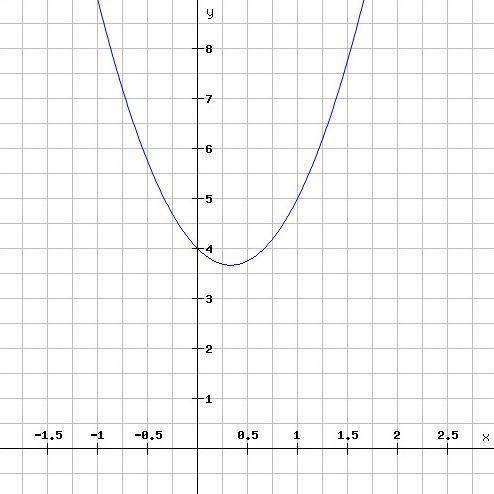
\includegraphics[width=9cm]{./_img/Polynom-Plot.jpeg}
        %    \centering \caption{Visualisierung des Graphen der Funktion $\R\to \R \ ,\ x\mapsto 3x^2-2x+4$}
        %\end{figure}
        \item Seien $\mathtt{cat}$ die Menge aller Katzen und $\mathtt{colour}$ die Menge aller Farben. Wir haben eine Abbildung
            \[ f: \mathtt{cat} \to \mathtt{colour} \ ,\ C \mapsto (\text{Die Fellfarbe von $C$}) \]
        deren Definitionsbereich genau $\mathtt{cat}$ und deren Wertebereich genau $\mathtt{colour}$ ist. Für eine Katze $C$ ist $f(C)$ genau die Fellfarbe von $C$.
        \item Sei $X$ eine beliebige Menge. Die Abbildung
            \[ \{-\}: X \to \calP(X) \ ,\ x \mapsto \{x\} \]
        hat als Definitionsbereich $X$, als Wertebereich die Potenzmenge von $X$ und sie ordnet jedem Element $x \in X$ diejenige Einermenge zu, die nur aus $x$ besteht.

        Der senkrechte Strich $-$ im Ausdruck „$\{-\}$“ meint einen Platzhalter, an dessen Stelle die Elemente des Definitionsbereichs „eingesetzt“ werden.
        \item Sei $\calA:=\{A\mid A\ \text{ist eine Aussage}\}$ die Menge aller mathematischen Aussagen. Die Junktoren $\land$ und $\neg$ ergeben Abbildungen
        \begin{align*}
            \calA\times \calA & \to \calA & \calA & \to \calA \\
            (A,B) & \mapsto A\land B & A& \mapsto \neg A
        \end{align*}
        d.h. im ersten Fall ordnen wir jedem Aussagenpaar $(A,B)$ die Konjunktion „$A$ und $B$“ zu und im zweiten Fall ordnen wir jeder Aussage ihre Negation zu. Ebenso liefern auch die anderen Junktoren $\lor,\to,\leftrightarrow$ jeweils Zuordnungen von Aussagen.
        \item Es bezeichne $\Set$ die Gesamtheit aller Mengen. Dann haben wir eine Abbildung
            \[ \Abb(-,-) : \Set \times \Set \to \Set \ ,\ (X,Y) \mapsto \Abb(X,Y) \]
        die jedem Mengenpaar $(X,Y)$ die Menge $\Abb(X,Y)$ aller Abbildungen $X\to Y$ zuordnet.
    \end{enumerate}
    Aus der Schule bist du es vielleicht gewohnt, dass der Graph einer Funktion eine Art „Kurve“ ist. Beachte, dass unsere allgemeine Graphendefinition deutlich abstrakter ist und der Graph einer Abbildung in der Regel keine „geometrische“ Bedeutung besitzt. Zumindest im Fall einer Abbildung $\R\to \R$ ist der Graph eine Teilmenge des $\R^2$, im Allgemeinen kann er aber alles andere als „kurvig“ aussehen.
\end{bsp}


\begin{vorschau}[* mengentheoretische Abbildungsdefinition]
    Die obige Definition einer Abbildung ist, ebenso wie die Mengendefinition \cref{def:menge}, rein axiomatisch. In der im 20. Jahrhundert vorherrschenden Praxis kann der Abbildungsbegriff formal präzise auf dem Mengen- und Elementbegriff aufgebaut werden: Eine Analyse ergibt, dass für zwei Abbildungen $f,g$ äquivalent sind:
    \begin{enumerate}[(i)]
        \item $f=g$.
        \item $\dom(f)=\dom(g)$, $\codom(f)=\codom(g)$ und $\graph(f)=\graph(g)$.
    \end{enumerate}
    \emph{Definiert} man nun eine Abbildung $f$ als ein Tripel $(X,G,Y)$ bestehend aus drei Mengen $X,G,Y$, wobei $G$ eine Teilmenge von $X\times Y$ mit der Eigenschaft, dass es für jedes $x\in X$ genau ein $y\in Y$ mit $(x,y)\in G$ gibt, sein soll, und definiert man $f(x):=(\text{das eindeutige $y\in Y$ mit $(x,y)\in G$})$ für jedes $x\in X$, so wird die Äquivalenz (i)$\leftrightarrow$(ii) zu einer beweisbaren Aussage, wohingegen sie in diesem Skript einfach als Axiom gegeben wurde.
    
    In der \href{https://en.wikipedia.org/wiki/Topos#Elementary_topoi_(topoi_in_logic)}{Topostheorie} wird umgekehrt verfahren: hier sind die „Abbildungen“ das fundamentale Konzept, das nicht definiert und nur durch Axiome beschrieben wird, worauf dann formal präzise die Begriffe von Element und Teilmenge aufgebaut werden.
    
    Weil ich keiner Herangehensweise den Vorzug geben will, werde ich es bei \cref{def:abbildung} belassen und nicht weiter auf eine formale Abbildungsdefinition eingehen.
\end{vorschau}


\begin{bem}[Beweisen, dass zwei Abbildungen gleich oder ungleich sind]
    Seien $X,Y$ zwei Mengen und $f,g:X\to Y$ zwei Abbildungen. Da das Gleichheitskriterium aus \cref{abbgleich} eine Allaussage ist (für \emph{jedes} $x\in X$ ist $f(x)=g(x)$), kann die Gleichheit $f=g$ nach \cref{allbeweis} dadurch bewiesen werden, dass ein „beliebiges“ Element von $X$ fixiert wird und dann bewiesen wird, dass dessen Funktionswerte unter $f$ und $g$ übereinstimmen.

    Bevor du überhaupt versuchst, die Gleichheit zweier Abbildungen zu beweisen, solltest du dich natürlich erstmal vergewissern, dass sie überhaupt denselben Definitionsbereich und denselben Wertebereich haben. Meistens ist das aber „offensichtlich“ und muss im Beweis nicht nochmal erwähnt werden.

    Um zu zeigen, dass die Abbildungen $f,g$ verschieden sind, genügt es nach \cref{gegenbeispiel}, ein Gegenbeispiel anzugeben, d.h. in diesem Fall, ein Element $x\in X$ zu finden, für das $f(x)\neq g(x)$.
\end{bem}


\begin{bsp} \label{bsp:abbgleich} \quad
    \begin{enumerate}
        \item Betrachten wir die Abbildungen: 
        \begin{align*}
            f: \R \to \R\ &,\ x \mapsto x^2 \\
            g: \R \to \R\ &,\ x \mapsto 2x+1
        \end{align*}
        So ist $f \neq g$, denn es ist $f(1)=1$ und $g(1)=3$.
        \item Betrachten wir dagegen die Abbildungen
        \begin{align*}
            \alpha: \R \to \R\ &,\ x \mapsto (x+1)\cdot (x-1) \\
            \beta: \R \to \R\ &,\ x \mapsto  x^2-1
        \end{align*}
        so gilt für jede beliebige reelle Zahl $x\in \R$, dass
            \[ \alpha(x) = (x+1)(x-1) = x^2-1 = \beta(x) \]
        Demnach ist $\alpha=\beta$.
    \end{enumerate}
\end{bsp}


\begin{bem}[Zuordnungsvorschriften vs. Abbildungen] \label{zuordvsabb}
    Jede Zuordnungsvorschrift kann zur Definition einer Abbildung verwendet werden. Beachte, dass Zuordnungsvorschriften und Abbildungen nicht ganz dasselbe sind. Eine Zuordnungsvorschrift ist ein sprachliches Gebilde, eine konkrete Vorschrift, wie Gegenständen vom Typ $X$ Gegenstände vom Typ $Y$ zuzuordnen seien, wohingegen der Abbildungsbegriff eine mathematische Abstraktion darstellt. Das Verhältnis zwischen Termen und Abbildungen ist, genau wie das zwischen Eigenschaften und Mengen (vgl. \cref{mengenvseig}), ein Aspekt der Dualität zwischen Syntax und Semantik (siehe \cref{syntaxvssemantik}).
    \begin{itemize}
        \item Dieselbe Abbildung kann durch verschiedene Zuordnungsvorschriften zustandekommen. Beispielsweise sind
        \begin{align*}
            \R \to \R \ &,\ x\mapsto x^2-1 \\
            \R \to \R \ &,\ x\mapsto (x+1)(x-1)
        \end{align*}
        zwei verschiedene Zuordnungsvorschriften, die aber nach \cref{bsp:abbgleich} dieselbe Abbildung darstellen.
        \item Nicht jede Abbildung muss durch eine einfache Zuordnungsvorschrift definierbar sein. Abbildungsvorschriften können beliebig kompliziert sein und manche Abbildungen sind so chaotisch, dass sie gar keiner Abbildungsvorschrift gehorchen. Beispielsweise beweist man in der Berechenbarkeitstheorie, dass es Abbildungen $\N \to \{0,1\}$ (also Abfolgen von Nullen und Einsen) geben muss, die nicht Turing-berechenbar\footnote{\href{https://de.wikipedia.org/wiki/Alan_Turing}{Alan Turing (1912-1954)}} sind, d.h. für die es keinen konventionellen Algorithmus gibt, der nacheinander alle Folgenglieder auflistet.
        \item Definitions- und Wertebereich sind grundlegende Bestandteile einer Abbildung. Beispielsweise kann der Ausdruck
            \[ x\mapsto x^2 \]
        in verschiedenfacher Weise als Zuordnungsvorschrift interpretiert werden, z.B. als Zuordnung $\R\to \R$, $\Z\to \N_0$ oder $\C\to \C$. Die drei Abbildungen
        \begin{align*}
            \R \to \R \ & ,\ x\mapsto x^2 \\
            \Z \to \N_0 \ & ,\ x\mapsto x^2 \\
            \C \to \C \ &,\ x\mapsto x^2 
        \end{align*}
        sind aber allesamt voneinander verschieden, da sie verschiedene Definitions- und Wertebereiche haben. Siehe auch \cref{bsp:injsur}.
    \end{itemize}
\end{bem}


\begin{bem}[Funktionen „in mehreren Variablen“]
    Nach unserer Abbildungsdefinition kann in eine Abbildung $f:X\to Y$ genau ein Element $x$ aus $X$ „eingesetzt“ werden, um genau ein Element $f(x)$ von $Y$ zu erhalten. Dies erweckt vielleicht den Anschein, dass unsere Abbildungsdefinition nicht in der Lage wäre, „Funktionen in mehreren Veränderlichen“ wie zum Beispiel
        \[ x,y \quad\mapsto\quad 2xy + xy^2 \]
    zu modellieren. -- Sie ist es aber, und der Trick besteht in der Verwendung des kartesischen Produkts als Definitionsbereich. Beispielsweise haben wir eine Abbildung
        \[ \R \times \R \to \R \ ,\ (x,y) \mapsto 2xy +xy^2 \]
    Abbildungen dieser Art sind das Hauptthema von \cref{kap:verknuepfungen}. Verwenden wir noch allgemeinere Produkte $\prod_{i\in I} M_i$ als Definitionsbereich, können wir auch „Funktionen in unendlich vielen Variablen“ definieren.
\end{bem}





\section{Verketten von Abbildungen}


\begin{defin}[Verketten von Abbildungen]\label{def:verkettung} \index{Verkettung von Abbildungen}
    Seien $X,Y,Z$ drei Mengen und $X\xrightarrow{f} Y$, $Y \xrightarrow{g} Z$ zwei Abbildungen. Mit
    \begin{align*}
        g\circ f && (\text{lies: „$g$ nach $f$“, „$g$ verkettet $f$“ oder „$g$ kringel $f$“})
    \end{align*}
    wird diejenige Abbildung $X\to Z$ bezeichnet, die gegeben ist durch die Zuordnungsvorschrift
    \begin{align*}
        X \to Z \ ,\ x \mapsto g(f(x))
    \end{align*}
    Die Abbildung $g\circ f$ heißt die \textbf{Verkettung}, \textbf{Komposition} oder \textbf{Hintereinanderausführung} von $f$ und $g$.
    
    Insgesamt erhalten wir eine Abbildung, die ein Paar von Abbildungen auf eine Abbildung abbildet:
        \[ \circ : \Abb(Y,Z)\times \Abb(X,Y) \to \Abb(X,Z) \ ,\ (g,f) \mapsto g\circ f\]
\end{defin}


\begin{bsp} \label{bsp:verkettung} \quad
    \begin{enumerate}
        \item Es seien $S:= \{ \text{Schauspieler in Filmen}\}$ die Menge aller Filmdarsteller und $F:=\{\text{Filme}\}$ die Menge aller Filme. Wir haben Abbildungen
        \begin{align*}
            f : S \to F \ & ,\ s\mapsto (\text{Der erste Film, in dem $s$ mitgespielt hatte}) \\
            g : F \to \N \ & ,\ x \mapsto (\text{Das Jahr, in dem die Dreharbeiten an $x$ begannen})
        \end{align*}
        Dann ist die Verkettung $g\circ f$ diejenige Abbildung $S\to \N$, die jedem Schauspieler das Jahr zuordnet, in dem der erste Film, bei dem er mitgespielt hat, gedreht wurde.
        \item Betrachte die Abbildungen
        \begin{align*}
            f : \R \to \R \ &,\ x\mapsto x^2 \\
            g : \R \to \R \ &,\ x \mapsto x-1
        \end{align*}
        Dann gilt für $x\in \R$:\footnote{vgl. \cref{bsp:substitution}}
        \begin{align*}
            (g\circ f)(x) & = g(f(x)) = g(x^2) = x^2-1 \\
            (f\circ g)(x) & = f(g(x)) = f(x-1) = (x-1)^2
        \end{align*}
        Wegen $(g\circ f)(4)\neq (f\circ g)(4)$ ist $g\circ f\neq f\circ g$.
    \end{enumerate}
\end{bsp}


\begin{bem} \quad
    \begin{itemize}
        \item Sind zwei Abbildungen durch Funktionsterme gegeben, so erhält man ihre Verkettung durch Einsetzen des einen Terms in den anderen im Sinne von \cref{def:substitution}, siehe dazu die nachfolgenden Beispiele. Dies ist ein Aspekt der Dualität zwischen Syntax und Semantik (siehe \cref{syntaxvssemantik}).
        \item Beachte, dass in der Notation „$g\circ f$“ diejenige Abbildung, die „zuerst“ ausgeführt wird, an rechter Stelle steht. Für ein Element $x \in X$ berechnet man $(g\circ f)(x)$, indem man zuerst $f(x)$ ausrechnet und darauf nun die Abbildung $g$ anwendet.
    \end{itemize}
\end{bem}


\begin{vorschau}[Integration durch Substitution]
    Die Technik, einer Abbildung $g$ eine Abbildung $f$ „vorzuschalten“, kennst du vielleicht schon aus der Schule als „Variablensubstitution“. Bei der sogenannten „Integration durch Substitution“ spielt dies eine maßgebliche Rolle. Sind $f,g:\R\to \R$ zwei hinreichend „glatte“ Funktionen und $a,b\in \R$, so besagt die Substitutionsregel, dass
        \[ \int_{f(a)}^{f(b)} g = \int_a^b (g\circ f) \cdot f' \]
    %Falls du diese Methode nicht kennst, ist das nicht schlimm. Sie wird üblicherweise in der Ana1- oder Ana2-Vorlesung thematisiert.
\end{vorschau}


\begin{satz}[Verketten von Abbildungen ist assoziativ] \label{abbassoziativ}
    Seien $A,B,C,D$ vier beliebige Mengen und
    \[\begin{tikzcd}
        A \ar[r, "f"] & B \ar[r, "g"] & C \ar[r, "h"] & D
    \end{tikzcd}\]
    drei Abbildungen. Dann gilt:
        \[ (h\circ g)\circ f = h\circ (g\circ f)\]
\end{satz}
\begin{proof}
    Für jedes $a \in A$ ist
    \begin{align*}
        \bigl((h \circ g) \circ f\bigr) (a)	& = \bigl(h \circ g\bigr) \bigl(f(a)\bigr) \\
        & = h\bigl(g(f(a))\bigr) \\
        & = h\bigl((g \circ f)(a)\bigr) \\
        & = \bigl(h \circ (g \circ f)\bigr)(a)
    \end{align*}
    Da das Element $a\in A$ beliebig gewählt war, folgt $(h\circ g)\circ f = h\circ (g\circ f)$.
\end{proof}


\begin{bem}[Klammern sparen] \label{abbklammerfrei}
    Aufgrund von \cref{abbassoziativ} wird in dessen Situation einfach
        \[ h\circ g\circ f \]
    geschrieben, da es egal ist, ob erst $g$ mit $f$ verkettet wird und dann $h$ mit $g\circ f$ -- oder ob erst $h$ mit $g$ verkettet wird und dann $f$ mit $h\circ g$. Mit fortgeschrittenen Techniken lässt sich zeigen, dass es auch bei Verkettungen von mehr als drei Abbildungen egal ist, wie man Klammern setzt. Daher werden Klammerungen meist ganz weggelassen.\footnote{vgl. dazu auch \cref{klammerfrei}} Sind etwa $A,B,C,D,E,F$ sechs Mengen und sind Abbildungen
    \[\begin{tikzcd}
        A \ar[r, "a"] & B \ar[r, "b"] & C \ar[r, "c"] & D \ar[r, "d"] & E \ar[r, "e"] & F
    \end{tikzcd}\]
    gegeben, so wird mit
        \[ e\circ d\circ c\circ b\circ a \]
    diejenige Abbildung notiert, die durch Verkettung dieser fünf Abbildungen entsteht, die sich also dadurch zusammensetzt, dass erst $a$ durchlaufen wird, dann $b$, dann $c$, dann $d$ und zuletzt $e$.
\end{bem}





\section{Identität und Inklusion}


Sei $X$ eine beliebige Menge. Gibt es überhaupt eine Abbildung $X\to X$? Solange wir keine Informationen über die Elemente von $X$ haben, können wir ja schwerlich eine besondere Abbildungsvorschrift angeben. Dennoch gibt es stets eine Abbildung $X\to X$, deren Zuordnungsvorschrift so simpel ist, dass man sie schon wieder übersehen könnte:


\begin{defin}[Identitätsabbildung] \index{Identität}
    Sei $X$ eine Menge. Die Abbildung
    \begin{align*}
        \id_X: X \to X \ ,\ x \mapsto x
    \end{align*}
    heißt die \textbf{Identität auf $X$}.
\end{defin}


\begin{bem}
    Die Identität auf der Menge $X$ bildet jedes Element auf sich selbst ab und „tut gar nichts“. Die Identität auf $\R$ kennst du auch schon aus der Schule: die Polynomfunktion „$f(x)=x$“ ist genau die Identitätsabbildung $\id_\R$ auf der Menge der reellen Zahlen.
\end{bem}


\noindent Der nächste Satz zeigt, dass sich die Identität hinsichtlich der Verkettung von Abbildungen verhält, wie die $0$ bei der Addition oder die $1$ bei der Multiplikation, vgl. \cref{def:neutrales}.


\begin{satz}[Neutralität der Identität] \label{idneutral}
    Seien $X,Y$ zwei beliebige Mengen und $X\xrightarrow{f} Y$ eine Abbildung. Dann gilt:
        \[ \id_Y \circ f = f \qquad\textnormal{und}\qquad f\circ \id_X = f \]
\end{satz}
\begin{proof}
    Für ein beliebiges Element $x \in X$ gilt:
    \begin{align*}
        (\id_Y \circ f)(x) & =\id_Y(f(x)) \\
        & = f(x)&& (\text{per Definition von $\id_Y$}) \\[0.5em]
        (f\circ \id_X)(x) & = f(\id_X(x)) \\
        & =f(x) && (\text{per Definition von $\id_X$})
    \end{align*}
    Da das Element $x\in X$ beliebig gewählt war, folgt $\id_Y\circ f=f$ und $f\circ \id_X=f$.
\end{proof}


\begin{vorschau}[* Die Kategorie der Mengen] \label{kategorien}
    \cref{idneutral} und \cref{abbassoziativ} lassen sich zusammenfassen in der Aussage, dass Mengen und Abbildungen die Struktur einer sogenannten \href{https://ncatlab.org/nlab/show/category}{Kategorie} bilden. Die Sprache der Kategorien ist von fundamentaler Bedeutung für die gesamte Mathematik und du wirst, falls du in die reine Mathematik gehst, in deinem Studium noch haufenweise weitere Kategorien kennenlernen. Zum Beispiel:
    \begin{longtable}{lccr}
    Fachgebiet & \phantom{Platzhalter} & Kürzel & \phantom{Platzhalterhalter} Kategorie \\
    \midrule
    Grundlagen && $\Set$ & Mengen \\ 
    && $\Pos$ & Geordnete Mengen \\[0.5em]
    Lineare Algebra && ${}_K\mathsf{Vec}$ & $K$-Vektorräume \\
    && ${}_R\mathsf{Mod}$ & $R$-Moduln \\
    && ${}_R\mathsf{Mat}$ & Matrizen über $R$ \\[0.5em]
    Analysis && $\mathsf{Top}$ & Topologische Räume \\
    && $\mathsf{Met}$ & Metrische Räume \\
    && $\mathsf{Man}$ & Mannigfaltigkeiten \\
    && $\sigma\textsf{-Alg}$ & Sigma-Algebren \\[0.5em]
    Algebra && $\Mon$ & Monoide \\
    && $\Grp$ & Gruppen \\
    && ${}_G\Set$ & $G$-Mengen \\
    && $\mathsf{Ring}$ & Ringe \\
    && ${}_R\mathsf{Alg}$ & $R$-Algebren \\[0.5em]
    Funktionalanalysis && $\mathsf{Unif}$ & Uniforme Räume \\
    && $\mathsf{Ban}$ & Banachräume \\
    && $\mathsf{Hilb}$ & Hilberträume \\[0.5em]
    Fortgeschrittene Vorlesungen && $\mathsf{Cat}$ & Kategorien \\
    && $\mathrm{Sh}(\calC)$ & Garben auf $\calC$ \\
    && $\Delta$ & Simplexkategorie \\
    && $\mathsf{sSet}$ & Simpliziale Mengen \\
    && $\mathrm{Ch}(\calA)$ & Komplexe in $\calA$ \\
    && $\mathsf{Sch}$ & Schemata \\
    \end{longtable}
\end{vorschau}


\begin{defin}[Inklusionsabbildung] \label{def:inklusion} \index{Inklusion (einer Teilmenge)}
    Seien $X$ eine Menge und $U\subseteq X$ eine Teilmenge. Die \textbf{Inklusionsabbildung} (oder auch kurz: \textbf{Inklusion}) von $U$ in $X$ ist die Abbildung
    \begin{align*}
        U \to X \ ,\ x \mapsto x
    \end{align*}
    Sie wird bevorzugt mit dem griechischen Buchstaben $\iota$ (iota) und einem Pfeil mit Haken „$\hookrightarrow$“ notiert:
        \[ \iota_U : U \hookrightarrow X \]
    Gelegentlich spricht man auch von der \emph{natürlichen Inklusion} oder der \emph{kanonischen Inklusion}.
\end{defin}


\begin{bem}
    Die natürliche Inklusion ordnet einem Element aus $U$ genau das gleiche Element in $X$ zu. Wie bei der Identitätsabbildung werden auch von der Inklusion keine Elemente verändert. Trotz ihres trivialen Abbildungsverhaltens erweist sich die Inklusionsabbildung für einige theoretische Überlegungen als nützlich, siehe z.B. \cref{bsp:quelleschrank} und \cref{pullbackrel}.
    
    Der „behakte Pfeil $\hookrightarrow$“ ist schlicht eine Variante zum gewöhnlichen Abbildungspfeil, die bei Abbildungen auftritt, die sich ähnlich wie die natürliche Inklusion verhalten. Er wird verwendet, um den „Inklusionscharakter“ einer Abbildung hervorzuheben.
\end{bem}


\begin{bsp}
    Wegen $\Z\subseteq\Q$ hat man eine Inklusionsabbildung $\Z \hookrightarrow \Q$.%, die jede ganze Zahl auf sich selbst, nun aufgefasst als rationale Zahl, abbildet.
\end{bsp}


\begin{comment}
\begin{bem}[„Kanonizizät“ der natürlichen Inklusion]
    Seien $X$ eine beliebige Menge und $U\subseteq X$ eine Teilmenge. Notiert man ohne weitere Spezifikation einen Pfeil „$U\hookrightarrow X$“, so ist damit in der Regel die natürliche Inklusion gemeint. Denn welche „selbstverständliche“ Abbildung sollte es, sofern dir keine weiteren Informationen über $X$ und $U$ bekannt sind, außer dass eben $U$ eine Teilmenge von $X$ ist, sonst noch von $U$ nach $X$ geben?
    
    Darin besteht das „Natürliche“ an der natürlichen Inklusion: dass man mit ihr völlig unabhängig von der konkreten Gestalt von $X$ und der Teilmenge $U$ stets eine konkrete Abbildung $U\to X$ zur Hand hat.
\end{bem}
\end{comment}


\begin{defin}[* Leere Abbildung] \index{Leere Abbildung}
    Sei $X$ eine beliebige Menge. Dann gibt es genau eine Abbildung $\emptyset\to X$, die sogenannte \textbf{leere Abbildung}. Es handelt sich genau um die natürliche Inklusion der leeren Teilmenge $\emptyset\subseteq X$.\footnote{vgl. \cref{leeremengeimmerdrin}}
\end{defin}





\section{Bilder und Urbilder von Teilmengen}


\begin{defin}[Bild und Urbild von Teilmengen] \label{def:bildmenge} \index{Faser} \index{Bild} \index{Urbild}
    Seien $X,Y$ Mengen und $X \xrightarrow{f} Y$ eine Abbildung.
    \begin{itemize}
        \item Die Menge
            \[ \im(f) := \{y\in Y\mid \exists x\in X:\ f(x)=y  \} \]
        heißt das \textbf{Bild von $f$} (englisch: ``image'').
        \item Für eine Teilmenge $A\subseteq X$ heißt
            \[ f(A) := \{ y \in Y \mid \exists a\in A:\ f(a)=y \} \]
        die \textbf{Bildmenge von $A$} oder schlicht das \textbf{Bild von $A$} unter $f$.
        \item Für eine Teilmenge $B\subseteq Y$ heißt
            \[ f^{-1}(B) := \{ x \in X \mid f(x)\in B \} \]
        die \textbf{Urbildmenge von $B$} oder schlicht das \textbf{Urbild} von $B$ unter $f$.
        \item Für ein Element $y\in Y$ heißt die Menge
            \[ f^{-1}(y) := \{ x\in X \mid f(x)=y \} \]
        die \textbf{Faser von $y$} (unter der Abbildung $f$). Man spricht auch vom \textbf{Urbild von $y$}. Die Elemente von $f^{-1}(y)$ werden ebenfalls \textbf{Urbilder von $y$} genannt.
    \end{itemize}
\end{defin}


\begin{bsp}
    Für die Abbildung
    \begin{align*}
        f: \Z \to \Z \ ,\ n \mapsto n^2
    \end{align*}
    gilt beispielsweise:
    \begin{align*}
        \im(f) & = \{n\in \N_0 \mid n\ \text{ist eine Quadratzahl} \} & f^{-1}(9) & = \{-3,3\} \\
        f(\Z_{\le 0}) & = f(\Z_{\ge 0}) = \im(f) & f^{-1}(0) & = \{0\} \\
        f(\{7\}) & = \{49\} & f^{-1}(-9) & = \emptyset \\
        f(\{2,6,-2,-5\}) & = \{4,25,36\} & f^{-1}(\{6,-1\}) & = \emptyset \\
        f^{-1}(\im(f)) & = \Z & f^{-1}(\{0,9,12\}) & = \{0,3,-3\}
    \end{align*}
\end{bsp}


\begin{bsp}[*] \quad
    \begin{enumerate}
        \item Für die Abbildung
            \[ f : \R \to \R \ ,\ x\mapsto x^5-x-1 \]
        wurde in \cref{bsp:exverwendung} gezeigt, dass $f^{-1}(0)\neq\emptyset$. Tatsächlich ist diese Faser sogar einelementig, ihr Element, also die eindeutige reelle Lösung der Gleichung $x^5-x-1=0$, lässt sich aber nicht mit herkömmlichen arithmetischen Operationen hinschreiben, vgl. \cref{zeichendefinieren}.
        \item In \cref{bsp:fallunterscheidung} wurde für die Abbildung
            \[ f : \N \to \N \ ,\ n \mapsto n\cdot (n+1) \]
        bewiesen, dass $\im(f)\subseteq \{n\in \N\mid n\ \text{ist gerade}\}$.
    \end{enumerate}
\end{bsp}


\begin{defin}[Konstante Abbildung] \index{konstante Abbildung}
    Seien $X,Y$ zwei Mengen. Eine Abbildung $X\xrightarrow{f} Y$ heißt \textbf{konstant}, wenn $\im(f)$ eine Einermenge ist, d.h. wenn es ein $y\in Y$ gibt derart, dass $f(x)=y$ für alle $x\in X$.
\end{defin}


\begin{bsp} \quad
    \begin{enumerate}
        \item Zum Beispiel ist
            \[ \R \to \R \ ,\ x\mapsto 4 \]
        die konstante Abbildung, die alles auf $4$ schickt. In der Analysis wird gezeigt, dass eine Abbildung $f : \R\to \R$ genau dann konstant ist, wenn sie differenzierbar ist mit $f'=0$.
        \item Allgemein geben Terme, die von gar keinen Variablen abhängen (siehe \cref{bsp:term}), Anlass zu konstanten Abbildungen.
        %\item Für eine Menge $X$ ist die leere Abbildung $\emptyset\to X$ keine konstante Abbildung, da ihr Bild leer ist und damit nicht einelementig. Die Handhabung ist in der Literatur aber nicht eindeutig: bei manchen sind auch leere Abbilungen konstant und die meisten verlieren hierüber gar kein Wort.
    \end{enumerate}
\end{bsp}





\section{Einschränkung von Definitions- oder Wertebereich}


In diesem Abschnitt seien stets $X,Y$ zwei Mengen und $f:X\to Y$ eine Abbildung.


\begin{defin}[Einschränken des Definitionsbereichs] \label{def:quelleschrank} \index{Restriktion}
    Sei $A \subseteq X$ eine Teilmenge von $X$. Dann ist die \textbf{Einschränkung von $f$ auf $A$} oder auch \textbf{Restriktion von $f$ auf $A$} diejenige Abbildung $A\to Y$, die durch die Abbildungsvorschrift
    \begin{align*}
        A \to Y \ &,\ a \mapsto f(a)
    \end{align*}
    gegeben ist. Notation:
    \begin{align*}
        f\vert_A && (\text{lies: „$f$ eingeschränkt auf $A$“})
    \end{align*}
    Die Abbildung $f\vert_{A}$ funktioniert also genau wie $f$, mit dem einzigen Unterschied, dass der Definitionsbereich verkleinert wurde und $f\vert_{A}$ nur noch den Elementen aus $A$ etwas zuordnet. Insgesamt erhalten wir eine sogenannte \emph{Restriktionsabbildung}:
        \[ \res : \Abb(X,Y) \to \Abb(A,Y) \ ,\ f \mapsto f\vert_A \]
    Beachte: Im Fall $A\subsetneq X$ sind $f$ und $f\vert_A$ zwei verschiedene Abbildungen, da sie verschiedene Definitionsbereiche haben.
\end{defin}


\begin{bsp} \label{bsp:quelleschrank} \quad
    \begin{enumerate}
    \item Betrachte die Abbildung
        \[ f : \R \to \R \ ,\ x \mapsto x^2 \]
    Deren Einschränkung auf die Teilmenge $\Q\subseteq \R$ ist dann gegeben durch
        \[ f\vert_{\Q} : \Q \to \R \ ,\ x\mapsto x^2 \]
    Obwohl die Zuordnungsvorschrift ($x\mapsto x^2)$ dieselbe ist, handelt es sich um eine andere Funktion! Beispielsweise ist $7\in \im(f)$ wegen $f(\sqrt{7})=7$; dagegen ist $7\notin \im(f\vert_\Q)$ denn es gibt keine rationale Zahl $q\in \Q$, für die $q^2=7$ wäre.
    \item Bezeichnet $\iota_A$ die Inklusion einer Teilmenge $A\subseteq X$, so gilt $f\vert_A = f\circ\iota_A$, d.h. die Restriktion ergibt sich durch Verketten mit der Inklusionsabbildung $A\hookrightarrow X$. Insbesondere ist die Inklusionsabbildung selbst $\iota_A = \id_X\circ \iota_A = \id_X \vert_A$ genau die Einschränkung der Identitätsabbildung auf $A$.
    \end{enumerate}
\end{bsp}
 
 
\begin{defin}[* Einschränkung und Fortsetzung] \label{def:fortsetzung} \index{Einschränkung einer Abbildung} \index{Fortsetzung}
    Seien $X,Y$ zwei Mengen, $A\subseteq X$ eine Teilmenge und $X\xrightarrow{F} Y$, $A\xrightarrow{f} Y$ zwei Abbildungen. $F$ heißt eine \textbf{Fortsetzung} von $f$ (und $f$ eine \textbf{Einschränkung} von $F$), wenn $F\vert_A=f$.
\end{defin}


\begin{bsp}[*] \quad
    \begin{enumerate}
        \item Die \emph{komplexe Betragsfunktion}
            \[ \C \to \R_{\ge 0} \ ,\ x+iy \mapsto \sqrt{x^2+y^2} \]
        ist eine Fortsetzung der reellen Betragsfunktion $\R\to \R_{\ge 0} \ ,\ x\mapsto \vert x\vert$.
        \item In der Analysis wird die Sprache der „Reihen“ entwickelt und bewiesen, dass durch
            \[ \zeta : \R_{>1} \to \C \ ,\ s \mapsto \sum_{n=1}^\infty \frac{1}{n^s} \quad =\  \frac{1}{1^s} + \frac{1}{2^s} + \frac{1}{3^s} + \frac{1}{4^s} + \frac{1}{5^s} + \ldots\]
        eine wohldefinierte Abbildung gegeben ist. Beispielsweise bewies Euler 1735, dass
            \[ 1 + \frac{1}{4} + \frac{1}{9} + \frac{1}{16} + \frac{1}{25} + \ldots = \zeta(2) = \frac{\pi^2}{6} \]
        und nach einem Satz von Apéry\footnote{\href{https://de.wikipedia.org/wiki/Roger Apery}{Roger Apéry (1916-1994)}} ist über die Zahl $\zeta(3)$ zumindest bekannt, dass sie irrational ist.

        Die Abbildung $\zeta$ besitzt unendlich viele verschiedene Fortsetzungen auf die Obermenge $\C \supseteq \R$, von denen die meisten aber völlig uninteressant sind. Allerdings wird in der Funktionentheorie gezeigt, dass $\zeta$ \emph{genau eine} Fortsetzung auf $\C\setminus \{1\}$ besitzt, die \emph{holomorph}, d.h. komplex differenzierbar, ist. Diese Fortsetzung wird ebenfalls mit dem Buchstaben „$\zeta$“ notiert und heißt die \emph{Riemannsche Zeta-Funktion}. Beispielsweise ist $\zeta(-1)=-\frac{1}{12}$. In der Unterhaltungsmathematik werden manchmal verblüffende „Beweise“ präsentiert für die Aussage, es gälte $1+2+3+4+5+\ldots = -\frac{1}{12}$.
    \end{enumerate}
\end{bsp}


\begin{defin}[* Einschränken des Wertebereichs] \label{def:zielschrank}
    Sei $B\subseteq Y$ eine Teilmenge mit $\im(f) \subseteq B$. Dann ist die \textbf{Einschränkung von $f$ auf $B$} diejenige Abbildung $X \to B$, die durch die Abbildungsvorschrift
    \begin{align*}
        X \to B \ ,\ x \mapsto f(x)
    \end{align*}
    gegeben ist. Notation:
    \begin{align*}
        f\vert^B && (\text{lies: „$f$ eingeschränkt auf $B$“})
    \end{align*}
    Die Abbildung $f\vert^B$ funktioniert also genau wie $f$, mit dem einzigen Unterschied, dass der Wertebereich verkleinert wurde.
\end{defin}


\begin{bsp}[*]
    Es seien $M := \{ x\mid x\ \text{steht in der Startelf des FC Bayern} \}$ sowie
        \[ f : M \to \R \ ,\ x \mapsto (\text{Das Jahresgehalt von $x$}) \]
    Dann ist $\im(f)\subseteq \R_{\ge 5.000.000}$, da (Stand 2021/22) jeder Spieler in der Startelf der Bayern ein Jahresgehalt von über fünf Millionen Euro bezieht\footnote{Quelle: \href{https://www.vermoegenmagazin.de/bayern-muenchen-gehaelter/}{vermoegenmagazin.de}. Beachte, dass die realen Einkommen dank Prämien und Werbeverträgen nochmal deutlich höher sind.}. Also lässt sich der Wertebereich von $f$ auf $\R_{\ge 5.000.000}$ einschränken, wodurch man die Abbildung
        \[ g: M \to \R_{\ge 5.000.000} \ ,\ x \mapsto (\text{Das Jahresgehalt von $x$}) \]
    erhält. $g$ und $f$ sind zwei verschiedene Abbildungen, weil sie verschiedene Wertebereiche haben.
\end{bsp}


\begin{bem}[*] \label{einschraenkbarkeit}
    Beachte, dass sich der Wertebereich einer Funktion $f$ nur auf solche Teilmengen einschränken lässt, die $\im(f)$ umfassen. Ist beispielsweise
        \[ f : \Z \to \Z \ ,\ n \mapsto 2n-n^2 \]
    so ergäbe der Ausdruck „$f\vert^{\N}$“ keinen Sinn. Denn die Zuordnung $n\mapsto 2n-n^2$ definiert keine Abbildung $\Z\to \N$, weil beispielsweise $2\cdot 5 - 5^2$ gar kein Element von $\N$ ist.

    Beim Definitionsbereich besteht keine solche Anforderung, er lässt sich auf beliebige Teilmengen einschränken.
\end{bem}





\section{Injektiv, surjektiv, bijektiv}


In diesem Abschnitt seien $X,Y$ stets zwei Mengen.


\begin{defin}[Injektive Abbildung] \label{def:injektiv} \index{injektiv}
    Eine Abbildung $X \xrightarrow{f} Y$ heißt \textbf{injektiv} (oder auch: eine \textbf{Injektion}), wenn sie eine (und damit jede) der folgenden äquivalenten Bedingungen erfüllt:
    \begin{enumerate}[(i)]
        \item Für alle $a,b\in X$ gilt:
            \[ f(a)=f(b) \quad\implies\quad a=b \]
        \item Für je zwei verschiedene Elemente $a,b \in X$ sind auch $f(a)$ und $f(b)$ voneinander verschieden.
        \item Für jedes $y\in Y$ gibt es höchstens ein $x\in X$ mit $f(x)=y$.
    \end{enumerate}
\end{defin}
\begin{proof}
    (i)$\leftrightarrow$(ii): Es ist (i) genau die Kontraposition von (ii) und damit zu (ii) äquivalent. \\[0.5em]
    (i)$\rightarrow$(iii): Es gelte (i) und es seien $a,b\in X$ mit $f(a)=y$ und $f(b)=y$. Wegen $f(a)=f(b)$ folgt aus (i), dass $a=b$. Also hat $y$ höchstens ein Urbild. \\[0.5em]
    (iii)$\rightarrow$(i): Seien $a,b\in X$ mit $f(a)=f(b)$. Da das Element $y:=f(a)\in Y$ nach (iii) höchstens ein Urbild hat, muss dann $a=b$ sein.
\end{proof}


\begin{bsp} Es gilt:
    \begin{enumerate}
        \item Die Abbildung
            \[ f:\Z \to \Z \ ,\ n \mapsto n^2-2n \]
        ist nicht injektiv, denn es ist $f(0)=f(2)$.
        \item Für eine beliebige Menge $X$ ist die Abbildung
            \[ X \to \calP(X) \ ,\ x \mapsto \{x\} \]
        injektiv. Denn sind $x,y\in X$ mit $\{x\}=\{y\}$, so ist bereits $x=y$.
        \item Sind $X$ eine beliebige Menge, $U\subseteq X$ eine Teilmenge und $\iota : U\to X$ die natürliche Inklusion, so ist $\iota$ eine injektive Abbildung, weil sie jedes Element auf sich selbst abbildet.
    \end{enumerate}
\end{bsp}
	

\begin{defin}[Surjektive Abbildung] \label{def:surjektiv} \index{surjektiv}
    Eine Abbildung $X \xrightarrow{f} Y$ heißt \textbf{surjektiv} (oder auch: eine \textbf{Surjektion}), wenn sie eine (und damit jede) der folgenden äquivalenten Bedingungen erfüllt:
    \begin{enumerate}[(i)]
        \item Für jedes $y\in Y$ gibt es mindestens ein $x\in X$ mit $f(x)=y$.
        \item Es gilt $\im(f) = Y$, d.h. das Bild von $f$ stimmt mit dem Wertebereich von $f$ überein.
    \end{enumerate}
\end{defin}
\begin{proof}
    Die Äquivalenz von (i) und (ii) ergibt sich direkt aus der Definition von $\im(f)$, siehe \cref{def:bildmenge}.
\end{proof}


\begin{bsp} \label{bsp:surjektiv}
    Es gilt:
    \begin{enumerate}
        \item Die Abbildung
            \[ \R \setminus \{2\} \to \R \setminus \{1\} \ ,\ x \mapsto \frac{x+1}{x-2} \]
        ist surjektiv. Dies wurde in \cref{bsp:allbeweis} bewiesen.
        \item Die Abbildung
            \[ f:\N_0 \to \N_0 \ ,\ n \mapsto n+1 \]
        ist zwar injektiv, jedoch nicht surjektiv. Denn es gibt keine natürliche Zahl $n\in \N_0$, für die $n+1=0$ gälte. Daher ist $0\notin \im(f)$ und $f$ ist nicht surjektiv. Dedekind\footnote{\href{https://de.wikipedia.org/wiki/Richard_Dedekind}{Richard Dedekind (1831-1916)}} erhob dieses Phänomen sogar zur Definition von Unendlichkeit: Eine Menge $X$ heißt \emph{Dedekind-unendlich}, wenn es eine injektive Abbildung $X\to X$ gibt, die nicht surjektiv ist.
        \item Die Abbildung
            \[ g: \N_0 \to \N_0\ ,\ n \mapsto \begin{cases}
                n-1 & n\ge 1 \\
                0 & n=0
            \end{cases}\]
        hingegen ist surjektiv (aber nicht injektiv), denn für jedes $n \in \N_0$ ist $n=g(n+1)$.
        \item Es sei $\bbP$ die Menge aller ungeraden Primzahlen. Goldbach\footnote{\href{https://de.wikipedia.org/wiki/Christian_Goldbach}{Christian Goldbach (1690-1764)}} vermutete 1742 in einem Briefwechsel mit Euler, dass sich jede gerade Zahl $\ge 4$ als Summe zweier Primzahlen schreiben lässt. Diese \href{https://de.wikipedia.org/wiki/Goldbachsche_Vermutung}{Goldbachsche Vermutung} ist äquivalent zu der Aussage, dass die Abbildung
            \[ \bbP \times \bbP \to \{n\in \N \mid n\ \text{ist gerade und}\ n\ge 6\} \ ,\ (p,q) \mapsto p+q \]
        surjektiv ist. Sie konnte bislang weder bewiesen noch widerlegt werden.
    \end{enumerate}
\end{bsp}


\begin{defin}[Bijektive Abbildung] \label{def:bijektiv} \index{bijektiv}
    Eine Abbildung $X \xrightarrow{f} Y$ heißt \textbf{bijektiv} (oder auch: eine \textbf{Bijektion}), wenn sie eine (und damit jede) der folgenden äquivalenten Bedingungen erfüllt:
    \begin{enumerate}[(i)]
        \item Für jedes $y\in Y$ gibt es genau ein $x\in X$ mit $f(x)=y$.
        \item $f$ ist injektiv und surjektiv.
    \end{enumerate}
\end{defin}
\begin{proof}
    $f$ ist genau dann injektiv, wenn es für jedes $y\in Y$ \emph{höchstens ein} $x\in X$ mit $f(x)=y$ gibt; und genau dann surjektiv, wenn es für jedes $y\in Y$ \emph{mindestens ein} $x\in X$ mit $f(x)=y$ gibt. Kombination beider Aussagen ergibt die Äquivalenz (i)$\Leftrightarrow$(ii).
\end{proof}


\begin{figure}[ht]
    \begin{minipage}{.48\textwidth}
        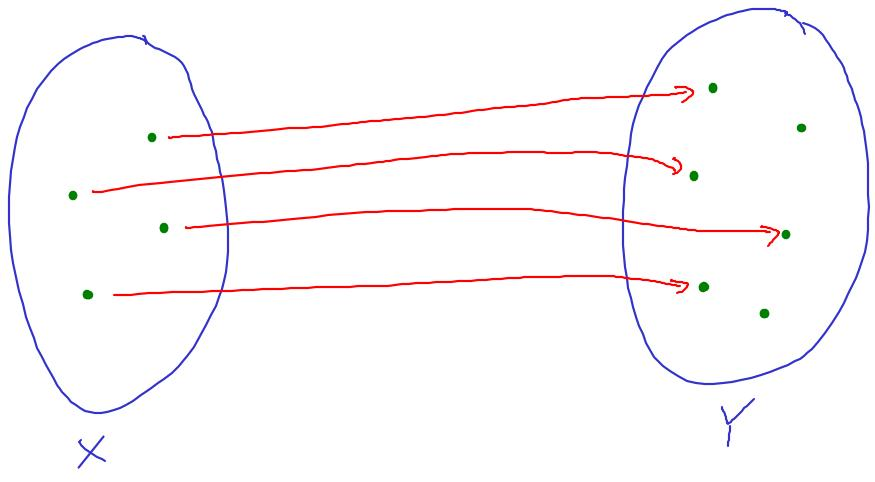
\includegraphics[width=7cm]{./_img/injsur4.jpeg}
        \centering \caption{injektiv, aber nicht surjektiv}
    \end{minipage}
    \quad
    \begin{minipage}{.48\textwidth}
        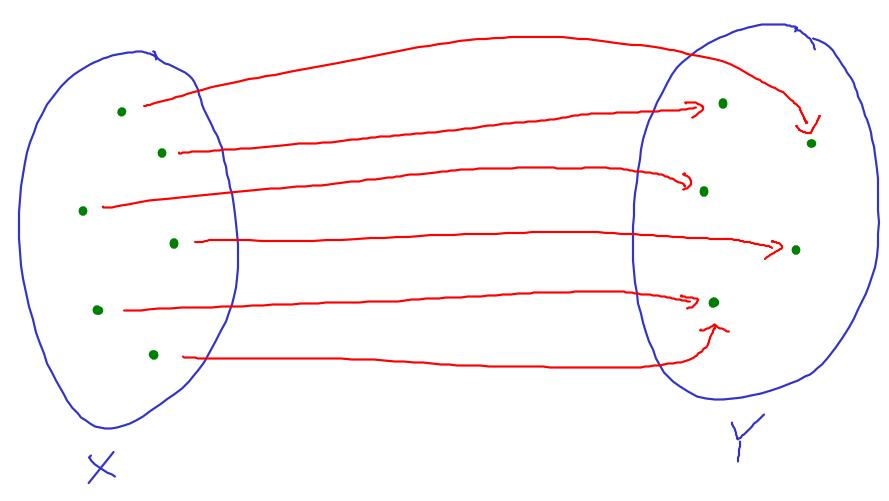
\includegraphics[width=7cm]{./_img/injsur2.jpeg}
        \centering \caption{surjektiv, aber nicht injektiv}
    \end{minipage}
    \quad\\[1em]
    \begin{minipage}{.48\textwidth}
        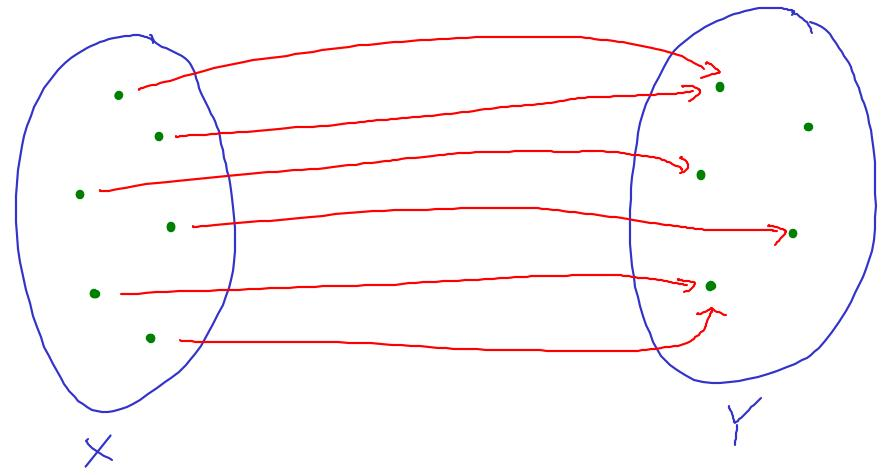
\includegraphics[width=7cm]{./_img/injsur1.jpeg}
        \centering \caption{weder injektiv noch surjektiv}
    \end{minipage}
    \quad
    \begin{minipage}{.48\textwidth}
        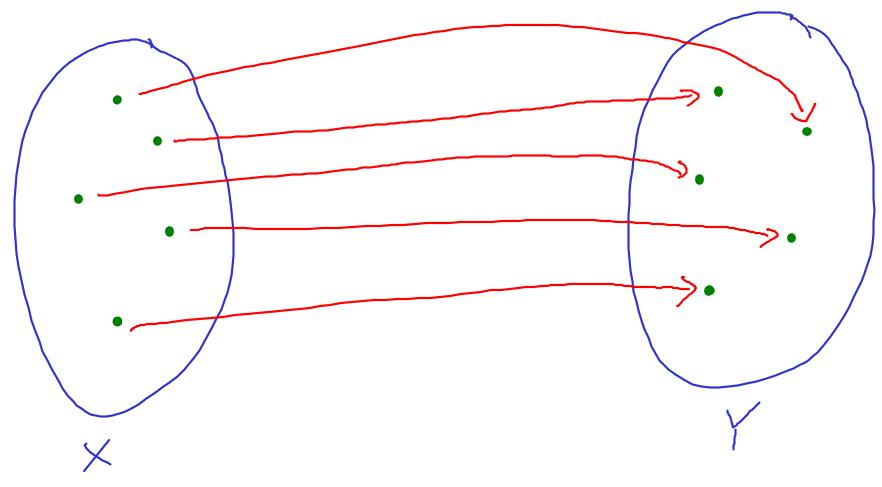
\includegraphics[width=7cm]{./_img/injsur3.jpeg}
        \centering \caption{bijektiv}
    \end{minipage}
\end{figure}


\begin{bsp} \label{bsp:injsur}
    Die vier Abbildungen
    \begin{align*}
        f_1 : \R \to \R \ &,\ x\mapsto x^2 & f_3 :\R\to \R_{\ge 0} \ &,\ x\mapsto x^2 \\
        f_2 : \R_{\ge 0} \to \R \ &,\ x\mapsto x^2 & f_4 :\R_{\ge 0} \to \R_{\ge 0} \ &,\ x\mapsto x^2
    \end{align*}
    sind, obwohl sie dieselbe Zuordnungsvorschrift haben, alle voneinander verschieden, weil sie verschiedene Definitions- oder Wertebereiche haben. Es gilt:
    \begin{enumerate}
        \item $f_1$ ist weder injektiv (wegen $f_1(1)=f_1(-1)$) noch surjektiv (wegen $-1\notin \im(f)$).
        \item $f_2$ ist injektiv (da jede reelle Zahl höchstens eines nichtnegative Quadratwurzel besitzt), aber nicht surjektiv.
        \item $f_3$ ist surjektiv (da jede nichtnegative reelle Zahl eine reelle Quadratwurzel besitzt), aber nicht injektiv.
        \item $f_4$ ist bijektiv. Denn jede nichtnegative reelle Zahl besitzt genau eine nichtnegative reelle Quadratwurzel.
    \end{enumerate}
\end{bsp}


\begin{vorschau}[Abbildungen künstlich surjektiv machen] \label{surjektivmachen}
    Seien $X,Y$ zwei Mengen und $f:X\to Y$ eine Abbildung. Gemäß \cref{def:zielschrank} lässt sich der Wertebereich von $f$ auf die Menge $\im(f)$ einschränken. Die dadurch erhaltene Abbildung
        \[ f\vert^{\im(f)} : X \to \im(f) \ ,\ x\mapsto f(x) \]
    ist automatisch surjektiv, da es ja für jedes $y\in \im(f)$ mindestens ein $x\in X$ mit $f(x)=y$ gibt.

    Auf diese Weise ist es uns gelungen, $f$ „künstlich surjektiv“ zu machen. Ist uns daran gelegen, mit surjektiven Abbildungen zu arbeiten, so stellt das also kein Problem dar, da wir den Wertebereich einer Abbildung stets auf ihr Bild einschränken können.

    Ebenso ist es möglich, die Abbildung $f$ „künstlich injektiv“ zu machen. Dabei besteht der Trick darin, zwischen solchen Elementen von $X$, die unter $f$ denselben Funktionswert haben, „nicht mehr zu unterscheiden“. Die Technik „ähnliche Elemente nicht mehr voneinander zu unterscheiden“ wird in der LA1 eine prominente Rolle im Umfeld des sogenannten \href{https://de.wikipedia.org/wiki/Homomorphiesatz}{Homomorphiesatzes} spielen und kann mithilfe der in \cref{kap:relationen} thematisierten \emph{Äquivalenzrelationen} formalisiert werden, siehe \cref{teilmengenvsfaktormengen}.
\end{vorschau}





\section{Invertierbare Abbildungen}


In diesem Abschnitt seien stets $X,Y$ zwei Mengen und $f:X\to Y$ eine Abbildung.


\begin{defin}[Umkehrabbildung] \label{def:umkehrabb} \index{Umkehrabbildung} \index{Inverse Funktion} \index{invertierbare Abbildung} \index{Retraktion}
    Eine Abbildung $g:Y \to X$ heißt 
    \begin{itemize}
        \item \textbf{linksinvers zu $f$} (oder auch: eine \textbf{Retraktion von $f$}), falls $g\circ f=\id_X$.
        \item \textbf{rechtsinvers zu $f$} (in manchem Kontext auch: ein \textbf{Schnitt von $f$}), falls $f\circ g=\id_Y$.
        \item \textbf{invers zu $f$} (oder auch: eine \textbf{Umkehrabbildung von $f$} oder eine \textbf{Inverse zu $f$}), falls sie sowohl links- als auch rechtsinvers zu $f$ ist.
    \end{itemize}
    $f$ heißt eine \textbf{invertierbare Abbildung}, wenn sie eine Umkehrabbildung besitzt.
\end{defin}


\begin{bsp} \label{bsp:umkehrabb} \qquad
    \begin{enumerate}
        \item Die Abbildung
            \[ \Z\to \Z \ ,\ n\mapsto n+1 \]
        ist invertierbar, eine Inverse ist gegeben durch die Abbildung $n\mapsto n-1$.
        \item Die „Spiegelung an der $x$-Achse“
        \[ \R^2 \to \R^2 \ ,\ (x,y) \mapsto (x,-y) \]
        ist zu sich selbst invers. Selbstinverse Abbildungen heißen auch \textbf{Involutionen}.
        \item Sei $X$ eine beliebige Menge. Aus \cref{idneutral} folgt $\id_X\circ \id_X=\id_X$, sodass $\id_X$ eine invertierbare, selbstinverse Abbildung ist.\footnote{vgl. \cref{regelnfuerinv}a)}
        \item Für $k\in \N_0$ betrachte die beiden Abbildungen
        \begin{align*}
            f:\N_0 \to \N_0 \ &,\ n \mapsto n+1 \\
            g_k: \N_0 \to \N_0\ &,\ n \mapsto \begin{cases}
                n-1 & n\ge 1 \\
                k & n=0
            \end{cases}
        \end{align*}
        Dann gilt
        \begin{align*}
            (g_k\circ f)(n)&=g_k(n+1)=n && n\in \N_0 \\
            (f\circ g_k)(0) & = f(k) = k+1 \neq 0
        \end{align*}
        sodass $g_k\circ f=\id_{\N_0}$ aber $f\circ g_k\neq \id_{\N_0}$. Also ist zwar $g_k$ linksinvers zu $f$ (und dementsprechend $f$ rechtsinvers zu $g_k$), aber nicht rechtsinvers zu $f$.
        \[\begin{tikzcd}
            f\vcentcolon & 0 \ar[r, bend left]& 1 \ar[r, bend left]& 2 \ar[r, bend left]& 3 \ar[r, bend left]& 4 \ar[r, bend left]& 5 \ar[r, bend left]& \dots \\
            g_0\vcentcolon & 0 \ar[loop, out=145, in=215, looseness=5] & 1 \ar[l, bend right] & 2 \ar[l, bend right] & 3 \ar[l, bend right] & 4  \ar[l, bend right] & 5  \ar[l, bend right] &  \ar[l, bend right]  \dots
        \end{tikzcd}\]
        Von weiteren Abbildungen dieser Art handelt die Geschichte vom \href{https://en.wikipedia.org/wiki/Hilbert\%27s_paradox_of_the_Grand_Hotel}{Hilbert-Hotel}.
    \end{enumerate}
\end{bsp}


\begin{satz}[Eindeutigkeit der Inversen]\label{umkehreind}
    Sei $f$ eine invertierbare Abbildung. Dann ist die Umkehrabbildung von $f$ eindeutig bestimmt.\footnote{vgl. \cref{inveind}}
\end{satz}
\begin{proof}
    Seien $g,h:Y\to X$ zwei Umkehrabbildungen von $f$. Dann gilt:
    \begin{align*}
        g & = g\circ \id_Y && (\text{nach \cref{idneutral}})\\
        & = g\circ (f\circ h) && (\text{da $h$ invers zu $f$ ist}) \\
        & = (g\circ f)\circ h && (\text{nach \cref{abbassoziativ}}) \\
        & = \id_X \circ h && (\text{da $g$ invers zu $f$ ist}) \\
        & = h && (\text{nach \cref{idneutral}}) 
    \end{align*}
    Also ist die Inverse von $f$ eindeutig bestimmt.
\end{proof}


\begin{bem}[\textbf{Die} Umkehrabbildung] \label{dieumkehrabb}
    Im Sinne von \cref{kennzeichnung} berechtigt uns dieser Eindeutigkeitssatz dazu, anstelle von „einer“ Umkehrabbildung von $f$ von \emph{der} Umkehrabbildung von $f$ zu sprechen.
    
    Die zu einer invertierbaren Abbildung $f$ inverse Abbildung wird notiert mit
        \[ f^{-1} \]
    Beachte, dass es nur nur dann Sinn ergibt, von „der Umkehrabbildung $f^{-1}$“ zu sprechen, wenn $f$ invertierbar ist. Im Allgemeinen sind Abbildungen nicht invertierbar und wir werden mit \cref{invwiderleg} Techniken herleiten, mit denen sich dies beweisen lässt.
\end{bem}


\begin{bem}
    Das Zeichen „$f^{-1}$“ ist bereits in \cref{def:bildmenge} aufgetaucht und bezeichnete dort Fasern und Urbildmengen. Ist $f$ invertierbar, so trägt es also drei verschiedene Bedeutungen zugleich. Hier ist eine Tabelle mit den verschiedenen Bedeutungen von „$f$“ und „$f^{-1}$“:
    \begin{center}
    \begin{tabular}{cl}
        Zeichen & Bedeutung \\
        \midrule
        $f$ & Die Abbildung $X \to Y \ ,\ x \mapsto f(x)$ \\
        $f$ & Die (mengenwertige) Abbildung $\calP(X) \to \calP(Y) \ ,\ A\mapsto f(A)$  \\
        $f^{-1}$ & Die (mengenwertige) Abbildung $\calP(Y) \to \calP(X) \ ,\ B\mapsto f^{-1}(B)$ \\
        $f^{-1}$ & Die (mengenwertige) Abbildung $Y \to \calP(X) \ ,\ y\mapsto f^{-1}(y)$ \\
        \midrule
        $f^{-1}$ & Die Umkehrabbildung $f^{-1} : Y\to X \ ,\ y \mapsto f^{-1}(y)$ \\
        & (existiert nur, wenn $f$ invertierbar ist)
    \end{tabular}
    \end{center}
    Beachte, dass die ersten vier Ausdrücke immer Sinn ergeben; der fünfte aber nur dann, wenn $f$ invertierbar ist.
\end{bem}


\begin{bem}
    Nach \cref{umkehreind} ist die Inverse einer invertierbaren Abbildung stets eindeutig bestimmt. Eine bloße Links- oder Rechtsinverse braucht dagegen nicht eindeutig sein, wie \cref{bsp:umkehrabb} zeigt.
\end{bem}


\begin{satz} \label{bijektiviso}
    Seien $X,Y$ zwei Mengen und $X\xrightarrow{f} Y$ eine Abbildung. Dann sind äquivalent:
    \begin{enumerate}[(i)]
        \item $f$ ist invertierbar.
        \item $f$ ist bijektiv.
    \end{enumerate}
\end{satz}
\begin{proof}
    (ii)$\to$(i): Sei $f$ bijektiv. Dann gibt es für jedes $y\in Y$ genau ein $x\in X$ mit $f(x)=y$, sodass durch
        \[ g : Y\to X \ ,\ y \mapsto (\text{Das eindeutig bestimmte $x\in X$ mit $f(x)=y$}) \]
    eine Abbildung definiert ist. $g$ ist invers zu $f$, denn: \\[0.5em]
    ($g\circ f=\id_X$): Für ein beliebiges $a\in X$ ist
    \begin{align*}
        (g\circ f)(a) = g(f(a)) = (\text{Das eindeutig bestimmte $x\in X$ mit $f(x)=f(a)$}) = a
    \end{align*}
    Weil $a\in X$ beliebig war, folgt die Gleichheit von Abbildungen $g\circ f=\id_X$. \\[0.5em]
    ($f\circ g=\id_Y$): Für ein beliebiges $b\in Y$ ist
    \begin{align*}
        (f\circ g)(b) = f(\text{Das eindeutig bestimmte $x\in X$ mit $f(x)=b$}) = b
    \end{align*}
    Also ist $f\circ g=\id_Y$. \\[0.5em]
    Insgesamt ist damit gezeigt, dass $g$ invers zu $f$ ist. \\[0.5em]
    Der Beweis der Implikation (i)$\to$(ii) ist Inhalt von \cref{aufg:bijektiviso}.
\end{proof}


\begin{bsp} \quad
    \begin{enumerate}
        \item Nach \cref{bsp:injsur} ist die Abbildung
            \[ \R_{\ge 0} \to \R_{\ge 0} \ ,\ x \mapsto x^2 \]
        bijektiv. Ihre Inverse wird mit „$\sqrt{-}$” notiert. Für $y\in \R_{\ge 0}$ ist also „$\sqrt{y}$“ die eindeutig bestimmte nichtnegative reelle Zahl, die die Gleichung $(\sqrt{y})^2=y$ erfüllt. Ebenso gilt auch $\sqrt{x^2}=x$ für alle $x\in \R_{>0}$ (sogar schon für alle $x\in \R$).
        \item Subtraktion, Division, Wurzel und Logarithmus sind jeweils invers zu Addition, Multiplikation und Potenz:
        \begin{center}
        \begin{tabular}{clll}
            Def.- und Wertebereich & Zuordnung & Inverse Zuordnung & \phantom{Platzhalter}\\
            \midrule
            $\R\to \R$ & $x\mapsto x+a$ & $x\mapsto x-a$ & (für $a\in \R$)\\
            $\R\to \R$ & $x\mapsto ax$ & $x\mapsto \frac{x}{a}$ & (für $a\in \R\setminus \{0\}$) \\
            $\R_{> 0} \to \R_{> 0}$ & $x\mapsto x^a$ & $x\mapsto \sqrt[a]{x}$ & (für $a\in \R\setminus \{0\}$) \\
            $\R \to \R_{>0}$ & $x \mapsto a^x$ & $x \mapsto \log_a(x)$ & (für $a\in \R_{>0}$)
        \end{tabular}
        \end{center}
        Du bist es ja aus der Schule gewohnt, Gleichungen, die Summen, Produkte und Potenzen enthalten, aufzulösen mittels Subtrahieren, Dividieren, Wurzelziehen und Logarithmieren.
    \end{enumerate}
\end{bsp}


\begin{bem}[Bijektivität beweisen]
    Ist $f$ eine Abbildung, für die du beweisen möchtest, dass sie bjektiv ist, so stehen dir nun zwei Wege offen:
    \begin{enumerate}
        \item Du arbeitest mit \cref{def:bijektiv}, d.h. du beweist sowohl, dass $f$ injektiv ist, als auch, dass $f$ surjektiv ist.
        \item Du arbeitest mit \cref{bijektiviso}, d.h. du schreibst einen Kandidaten für die Umkehrabbildung hin und beweist daraufhin, dass er tatsächlich invers zu $f$ ist.
    \end{enumerate}
    Es gibt Situationen, in denen es schwer bis unmöglich ist, eine konkrete Abbildungsvorschrift für eine Umkehrabbildung anzugeben. In diesem Fall ist der erste Weg leichter.
    
    Es gibt aber auch Situationen wie z.B. in \cref{bsp:umkehrabb}, in denen du bei genauem „Hinsehen“ bereits einen Kandidaten für eine Umkehrabbildung ausfindig machen kannst. In diesem Fall bietet sich der zweite Weg an. Beachte auch, dass ein Beweis über den zweiten Weg stets informativer ist, da er dem Leser bereits die Gestalt der inversen Abbildung mitteilt.
\end{bem}


\begin{bem}[Invertierbarkeit widerlegen] \label{invwiderleg}
    Möchtest du beweisen, dass eine Abbildung keine Umkehrabbildung besitzt, so genügt es nach \cref{bijektiviso} bereits, wenn du beweist, dass sie nicht injektiv oder nicht surjektiv ist.
\end{bem}


\begin{bsp}
    Beispielsweise gilt:
    \begin{enumerate}
        \item Die Abbildung $f : \R \to \R \ ,\ x\mapsto x^2$ ist nicht invertierbar, weil sie nicht injektiv ist. Denn es ist zum Beispiel $f(-5)=f(5)$.
        \item Die Abbildung $f : \N_0 \to \N_0 \ ,\ n \mapsto n+1$ ist nicht invertierbar, weil sie nicht surjektiv ist. Denn es ist $0\notin \im(f)$.
    \end{enumerate}
\end{bsp}





\clearpage
\section{Aufgabenvorschläge}


\begin{aufg}[Zerlegen von Abbildungen]
    Realisiert die folgenden Abbildungen als Verkettung möglichst elementarer Bausteine:
    \begin{enumerate}
        \item $\R\to \R \ ,\ x\mapsto (3x+1)^3$
        \item Sei $A$ die Menge aller Leute im Tutorium. Betrachte die Abbildung $f:A\to \N \ ,\ a\mapsto$ (die Anzahl der Wörter im Erstlingswerk des Literaturnobelpreisträgers im Geburtsjahr von $a$).
        \item $\calP(\R) \to \calP(\Q) \ ,\ X \mapsto \Q \setminus (X^c\cap \Z)$
        %\item $\N \to \N \ ,\ n \mapsto 3^n + n$\quad(schwierig)
    \end{enumerate}
\end{aufg}


\begin{aufg}[Wohldefiniertheit] \label{aufg:wohldef}
    An der Tafel von Captain Chaos stehen die folgenden Ausdrücke:
    \begin{align*}
        & (i) & \N \to \N\ &,\ n \mapsto n-1 \\[0.5em]
        & (ii) & \R\times \R \to \R \ &,\ (x,y) \mapsto \frac{x}{y} \\[0.5em]
        & (iii) & \R \times \R \to \R \ &,\ (x,y) \mapsto x^y \\[0.5em]
        & (iv) & \Q \to \Z \ &,\ \frac{p}{q} \mapsto p-q \\
        & (v) & \R \to \R \ &,\ x \mapsto \begin{cases}
            x^2+1\ , & \text{falls}\ x \le 0 \\
            x^2-1\ , & \text{falls}\ x\ge 0
        \end{cases}
    \end{align*}
    Was haltet ihr davon?
\end{aufg}


\begin{aufg}[injektiv, surjektiv, bijektiv]
    Untersucht die folgenden Abbildungen darauf, ob sie injektiv, surjektiv oder bijektiv sind:
    \begin{align*}
        & \text{a)} & \Z \to \Z\ &,\ n\mapsto 2n \\
        & \text{b)} & \Z \times \N_{\ge 1} \to \Q\ &,\ (z,n) \mapsto \frac{z}{n} \\
        & \text{c)} & \R \to \R\ &,\ x\mapsto 3x+1 \\
        & \text{d)} & \calP(\R) \to \calP(\R) \ &,\ A \mapsto A^c \\
        & \text{e)} & X\xrightarrow{\id} X\ & && (\text{für eine beliebige Menge $X$}) \\
        & \text{f)} & X\times Y \to X \ &,\ (x,y) \mapsto x && (\text{für beliebige Mengen $X,Y$})
    \end{align*}
\end{aufg}


\begin{aufg}[Vererbung von Injektivität und Surjektivität] \label{aufg:bijektiviso}
    Seien $X,Y,Z$ drei beliebige Mengen und $X \xrightarrow{f} Y \xrightarrow{g} Z$ zwei Abbildungen. Beweist die folgenden Implikationen:
    \begin{enumerate}
        \item $f,g$ injektiv $\implies$ $g\circ f$ injektiv $\implies$ $f$ injektiv.
        \item $f,g$ surjektiv $\implies$ $g\circ f$ surjektiv $\implies$ $g$ surjektiv.
        \item Invertierbare Abbildungen sind bijektiv.
    \end{enumerate}
    %Könnt ihr euch a) und b) im Beweis von c) zunutze machen?
\end{aufg}


% ====================================================================
%                                                                 
%
%       §01
%
%
% %%ts latex start%%[2019-03-07 Thu 14:45]%%ts latex end%%
% ====================================================================


% --------------------------------------------------------------------
% §1.1 section <<Begriff der Relation>>
% --------------------------------------------------------------------
\section{Begriff der Relation}

Im letzten Kapitel haben wir Ausdrücke der Form $f(x)=x^3$ in \textit{Abbildungen} $f:A\to B$ verallgemeinert, die eine Beziehung zwischen den Elementen einer Menge $A$ und einer Menge $B$ herstellen. Heute möchten wir Ausdrücke wie $2\leq 3$ oder $\sqrt{2}\neq \sqrt{3}$, die Beziehungen zwischen je zwei Elementen der selben Menge angeben, als \textit{Relationen} realisieren. Relevant sind vor allem \textit{Ordnungsrelationen} und \textit{Äquivalenzrelationen}.

% Definition Relation
Abstrakt kodieren wir für den Relationenbegriff die Elemente, die in Beziehung
stehen sollen, in einem Paar, also einem Element des kartesischen
Produkts.
\begin{de}
	Sei $X$ eine Menge. Eine \textbf{Relation} $\sim$ auf $X$ ist verkörpert durch eine Teilmenge $R\subseteq X\times X$ mit
\begin{align*}
 x\sim y\quad :&\Leftrightarrow\quad (x,y)\in R && x,y\in X
\end{align*}
\end{de}

%\begin{bsp}\label{bsp:gatsby}
%	Auf der Menge $X=\{\text{Nick Carraway, Jay Gatsby, Daisy Buchanan, Thomas Buchanan}\}$ betrachten wir die Relation \glqq\,$\_$ liebt $\_$\grqq\,. Wir haben $N$ liebt $J$, $D$ liebt $J$, $J$ liebt $D$ und $T$ liebt $D$.
%		\[ \begin{tikzcd}
%			N \ar[r] & J \ar[d,leftrightarrow]\\ T \ar[r] & D
%		\end{tikzcd} \]
%	Die kodierende Menge $R\subset X\times X$ ist also
%		\[ R = \left\{(N,J),(J,D),(D,J),(T,D)\right\} \,. \]
%\end{bsp}

\begin{bsp}\label{bsp:starwars}
	Auf der Menge $X=\{$Luke Skywalker, Anakin Skywalker, Yoda, Obi-Wan Kenobi, Qui-Gon Jinn, Dooku, Palpatine, Darth Maul, Darth Plagueis$\}$ betrachten wir die Relation
		\[ x \sim y :\Longleftrightarrow \text{ $x$ war Padawan von $y$. } \]
	Wir haben
		\[\begin{tikzcd}
			&		& \text{Darth Plagueis} & \\
			& \text{Yoda} & \text{Palpatine} \ar[u] & \\
			& 		& \text{Dooku}\ar[u]\ar[ul] & \text{Darth Maul}\ar[ul] \\
			&		& \text{Qui-Gon Jinn} \ar[u] &\\
			&		& \text{Obi-Wan Kenobi} \ar[u] & \\
			& \text{Luke Skywalker}\ar[uuuu]\ar[ur]	& &\text{Anakin Skywalker}\ar[ul]\ar[uuuul]
		\end{tikzcd}\]
	Ein Pfeil von $a$ nach $b$ soll dabei dafür stehen, dass $a$ mit $b$ in Beziehung $a\sim b$ steht, also $a$ ein Padawan von $b$ war. Eine solche Darstellung nennt man einen \textbf{Graphen} der Relation.
	
	Die kodierende Menge $R\subset X\times X$ ist also $R = \big\{$(Luke,Yoda), (Luke,Obi-Wan), (Anakin,Obi-Wan), (Anakin, Palpatine), (Obi-Wan,Qui-Gon), (Qui-Gon, Dooku), (Dooku, Yoda), (Dooku, Palpatine) (Darth Maul, Palpatine), (Palpatine, Darth Plagueis)$\big\}$.
\end{bsp}

\begin{bsp}\label{bsp:leq}
	Auf $\Zz$ definieren die Relation \glqq$\leq$\grqq\, durch
\begin{align*}
 n\leq m \quad &:\Leftrightarrow\quad \exists k\in\mathbb{N}_0: m=n+k  && n,m\in \Zz
\end{align*}
	Durch welche Menge $R\subset\Zz\times\Zz$ wird \glqq$\leq$\grqq\, repräsentiert? Für $n,m\in \Zz$ gilt: 
		\[ (n,m)\in R\quad \overset{!}{\Leftrightarrow}\quad n\leq m \quad\Leftrightarrow\quad \exists k\in\mathbb{N}_0: m=n+k \,. \]
	Eine mögliche Formulierung wäre also \( R = \left\{(n,m)\in\Zz\times\Zz\mid\exists k\in\mathbb{N}_0: m=n+k\right\} \). Letztlich haben wir hier einfach nur die Definition der Relation abgeschrieben und nicht wirklich etwas gelernt; wenn man tatsächlich mit Relationen arbeitet, ist es ganz allgemein meist ergiebiger, die Menge $R$ als technische Umsetzung zu vergessen und sich mit der direkten Definition der Relation auseinanderzusetzen. Wie das gemeint ist, sehen wir gleich bei den Eigenschaften von Relationen.
\end{bsp}

\begin{de}\label{bsp:trivialrelationen}
	Vorher noch drei Extrembeispiele: Sei $X$ eine beliebige Menge.
\begin{itemize}
 \item Die \textbf{Allrelation} auf $X$ ist verkörpert durch die Menge $X\times X$, setzt also alle Elemente miteinander in Beziehung:
		\[ \begin{tikzcd}[column sep = huge]
			x \ar[loop] \ar[r,<->] \ar[rr, out=320, in=220, <->] &
			y \ar[loop] \ar[r,<->]  &
			z \ar[loop] 
		\end{tikzcd} \]
	Die Doppelpfeile stehen dabei für eine Beziehung in beide Richtungen, etwa gilt $x\sim y$ sowie $y\sim x$.
\item Die \textbf{Nullrelation} ist verkörpert durch die leere Menge $\emptyset$, setzt also keine Elemente in Beziehung:
		\[ \begin{tikzcd}[column sep = huge]
			 x &y &z &  
		\end{tikzcd} \]
\item Die \textbf{Gleichheitsrelation} ist definiert durch $x\sim y:\Leftrightarrow x=y$, also
		 \[ \begin{tikzcd}[column sep = huge]
		 	x \ar[loop] &
		 	y \ar[loop] &
		 	z \ar[loop] 
		 \end{tikzcd} \]
	Sie ist verkörpert durch die so genannte \emph{Diagonale}
		\[ D_X :=\left\{ (x,x)\in X\times X\mid x\in X \right\} \,. \]
	(In der Darstellung des kartesischen Produkts als Ebene mit Koordinatenachsen ist das gerade die Winkelhalbierende, daher der Name.)
\end{itemize}
\end{de}

\begin{de}
	Sei $X$ eine Menge und $\sim$ eine Relation auf $X$. Dann heißt die Relation $\sim$
	\begin{itemize}
		\item \textbf{reflexiv}, falls für alle $x\in X$ die Relation $x\sim x$ gilt. Im Graphen muss jedes Element also einen Pfeil von sich auf sich selbst tragen.
		\item \textbf{symmetrisch}, falls für alle $x,y\in X$ aus $x\sim y$ schon $y\sim x$ folgt. Im Graphen müssen also alle Pfeile zwischen verschiedenen Elementen Doppelpfeile sein.
		\item \textbf{antisymmetrisch}, falls für alle $x,y\in X$ aus $x\sim y$ und $y\sim x$ schon $x=y$ folgt.	Im Graphen darf es also zwischen verschiedenen Elementen keine Doppelpfeile geben.
		\item \textbf{transistiv}, falls für alle $x,y,z\in X$ aus $x\sim y$ und $y\sim z$ schon $x\sim z$ folgt. Im Graphen gibt es für einen indirekten Weg entlang der Pfeile auch immer den direkten.
	\end{itemize}
	\begin{figure}[h]
		\begin{tikzpicture}[commutative diagrams/every diagram]
			\begin{scope}[xshift=-6cm]
				\node (P0) at (0,0) {$x$};
				\path[commutative diagrams/.cd, every arrow, every label]
				(P0) edge[commutative diagrams/loop] (P0);
				\node[below] at (0,-.5) {reflexiv};
			\end{scope}
			\begin{scope}[xshift=-2cm]
				\node (P0) at (-.7,0) {$x$};
				\node (P1) at (.7,0) {$y$};
				\path[commutative diagrams/.cd, every arrow, every label]
				(P0) edge[commutative diagrams/<->] (P1);
				\node[below] at (0,-.5) {symmetrisch};
			\end{scope}
			\begin{scope}[xshift=2cm]
				\node (P0) at (-.7,0) {$x$};
				\node (P1) at (.7,0) {$y$};
				\path[commutative diagrams/.cd, every arrow, every label]
				(P0) edge[commutative diagrams/<->] (P1);
				\draw (-.3,-.3) -- (.3,.3);
				\node[below] at (0,-.5) {antisymmetrisch};
			\end{scope}
			\begin{scope}[xshift=6cm]
				\node (P0) at (-1.3,.5) {$x$};
				\node (P1) at (0,0) {$y$};
				\node (P2) at (1.3,.5) {$z$};
				\path[commutative diagrams/.cd, every arrow, every label]
				(P0) edge (P1)
				(P1) edge (P2)
				(P0) edge[commutative diagrams/dotted, out=20, in=160] (P2);
				\node[below] at (0,-.5) {transitiv};
			\end{scope}
 		\end{tikzpicture}
	\end{figure}
\end{de}



\begin{bem}
 Die Definition einer symmetrischen Relation kann als die Formel
 \begin{align*}
  x\sim y\quad & \implies\quad y\sim x && x,y\in X
 \end{align*}
formuliert werden. Dies impliziert bereits die Äquivalenz
 \begin{align*}
  x\sim y\quad & \Leftrightarrow\quad y\sim x && x,y\in X
 \end{align*}
 da „$x$“ und „$y$“ ja austauschbare Bezeichnungen für beliebige Elemente von $X$ sind.
\end{bem}


\begin{bsp}\label{bsp:relationseigenschaften}
	Wir prüfen die Padawan-Relation aus \cref{bsp:starwars} auf diese Eigenschaften:
		\begin{itemize}
			\item Sie ist nicht reflexiv, etwa war Obi-Wan nicht sein eigener Padawan (tatsächlich gilt das für kein $x\in X$).
			\item Sie ist nicht symmetrisch, etwa war Luke Yodas Padawan, aber Yoda nicht Lukes.
			\item Sie ist antisymmetrisch, denn es gibt keine $x,y\in X$ mit $x\sim y$ und $y\sim x$; daher ist die Implikation
				\[ \forall x,y\in X : \big(\underbrace{x\sim y \text{ und }y\sim x}_\text{falsch}\implies x=y\big) \]
			trivialerweise eine wahre Aussage (\textit{ex falso quod libet}, siehe auch \cref{vacuoustruth}).
			\item Sie ist nicht transitiv, denn es war Darth Maul Padawan von Palpatine, und Palpatin Padawan von Darth Plagueis, aber Darth Maul nicht Padawan von Darth Plagueis.
		\end{itemize}
	Für die $\leq$-Relation aus \cref{bsp:leq} gilt:
		\begin{itemize}
			\item Sie ist reflexiv, denn für alle $n\in\Zz$ gilt $n\leq n$ (setze $k=0$).
			\item Sie ist nicht symmetrisch, so ist etwa $2\leq3$ aber $3\not\leq2$.
			\item Sie ist antisymmetrisch, denn aus $n\leq m$ und $m\leq n$ folgt $n=m+k_1$ und $m=n+k_2$. Setzen wir ein, erhalten wir $n=n+k_1+k_2$, also $k_1+k_2=0$. Wegen $k_1,k_2\geq0$ folgt $k_1=k_2=0$ und daher $n=m$.
			\item Sie ist transitiv, denn: Sei $n\leq m$ und $m\leq k$, etwa $m=n+k_1$ und $k=m+k_2$. Dann gilt
				\[ k=m+k_2=n+\underbrace{k_1+k_2}_{=:k_3} \]
				und wegen $k_3=k_1+k_2\in\mathbb{N}_0$ folgt daraus gerade $n\leq k$.
		\end{itemize}
\end{bsp}



\begin{bem}[Die tiefere Bedeutung der Transitivität] \label{kettenfalten}
 Seien $X$ eine Menge mit einer Relation „$\sim$“ und $a,b,c,d\in X$ ein paar Elemente von $X$. Anstelle von „Es gilt $a\sim b$, $b\sim c$ und $c\sim d$“ schreibt man kurz einfach
 \[ a\sim b\sim c\sim d \]
 Beispielsweise schreibt man
 \[ \Nz \subseteq \Zz\subseteq\Qz\subseteq\Rz\subseteq \Cz \]
 oder
 \[ 2 < 4 < 8 < 12 < 15 \]
 Mit dieser Notation lässt sich die Definition der Transitivität auch durch folgende Formel ausdrücken:
 \begin{align*}
  x\sim y \sim z \quad&\implies\quad x\sim z && x,y,z\in X
 \end{align*}
Transitivität heißt also, dass sich jede aus drei Elementen bestehende „Relationskette“ „zusammenfalten“ lässt. Es lässt sich zeigen, dass dies bei transitiven Relationen auch für beliebig lange „Ketten“ gilt. Mit anderen Worten: Sind $n\in \Nz$ und $x_1,\dots , x_n\in X$ ein paar Elemente mit
\[ x_1 \sim x_2\sim \ldots \sim x_n \]
so folgt, sofern ${\sim}$ eine transitive Relation ist, daraus auch schon $x_1\sim x_n$. Im Spezialfall, dass $\sim$ die Gleichheitsrelation ist, hast du das auch schon in der Schule andauernd ausgenutzt: Sind $x_1,\dots , x_n$ irgendwelche Zahlen/Vektoren/Funktionen und gilt
\[ x_1=x_2\ldots = x_n \]
so folgt daraus, dass auch $x_1=x_n$ ist. \\[0.5em] 
 Beachte, dass diese Schlussfolgerung bei nicht-transitiven Relationen fehlschlägt. Beispielsweise gilt
 \[ 2\cdot 6 \neq 3\cdot 6\neq 3\cdot 4 \]
 aber es ist ja dennoch $2\cdot 6=3\cdot 4$.
\end{bem}

% --------------------------------------------------------------------
% §1.2 section <<Ordnungsrelationen>>
% --------------------------------------------------------------------
\section{Ordnungsrelationen}

Ordnungsrelationen sind Verallgemeinerungen der bekannten \glqq$\leq$\grqq-Relation auf den Zahlenräumen $\mathbb{N},\mathbb{Z},\mathbb{Q},\mathbb{R}$ und werden daher häufig mit dem Symbol $\leq$ anstelle von $\sim$ notiert, auch wenn es nicht zwingend um Zahlenräume geht.

\begin{de}[Ordnungsrelationen]
	Eine \textbf{Ordnungsrelation} (auch: \swdde{partielle Ordnung} oder \emph{Halbordnung}) auf einer Menge $X$ ist eine Relation $\leq$ auf $X$, die reflexiv, antisymmetrisch und transitiv ist. Konkret:
\begin{align*}
 & (\text{O1}) & \forall x\in X:&\quad x\leq x && (\text{Reflexivität}) \\
& (\text{O2}) & \forall x,y\in X:&\quad  x\leq y\ \wedge\  y\leq x \quad\implies\quad x=y && (\text{Antisymmetrie}) \\
& (\text{O3}) & \forall x,y,z\in X:&\quad x\leq y\ \wedge\ y\leq z \quad\implies\quad x\leq z && (\text{Transitivität})
 \end{align*}
In diesem Fall nennt man das Paar $(X,\leq)$ eine \textbf{geordnete Menge}.

Besitzt die Ordnungsrelation „$\leq$“ sogar die Eigenschaft
\begin{align*}
 & (\text{TO}) & \forall x,y \in X:&\quad x\leq y\ \vee\ y\leq z 
\end{align*}
so nennt man sie eine \textbf{Totalordnung}. Eine Totalordnung ist also eine Halbordnung, bei der je zwei Elemente miteinander \glqq vergleichbar\grqq\, sind.
\end{de}

\begin{bsp} Es gilt:
\begin{itemize}
 \item Die Padawan-Relation aus \cref{bsp:starwars} ist keine Halbordnung, denn in \cref{bsp:relationseigenschaften} haben wir gesehen, dass sie nicht transitiv (und auch nicht reflexiv) ist.
 \item Die $\leq$-Relation aus \cref{bsp:leq} dagegen ist nach \cref{bsp:relationseigenschaften} tatsächlich eine Halbordnung. Es liegt sogar eine Totalordnung vor, denn: Seien $m,n\in\Zz$. Dann gilt entweder $m-n\geq0$ oder $m-n<0$. Im ersten Fall setze $k=m-n\in\mathbb{N}_0$ und erhalte aus $m=n+k$ schon $n\leq m$. Im zweiten Fall setze $k=n-m=-(m-n)\in\mathbb{N}_0$ und erhalte aus $n=m+k$ schon $m\leq n$.
\end{itemize}
\end{bsp}

\begin{bsp}[Teilmengenrelation]
	Sei $M$ eine Menge. Auf $\cP(M)$ betrachten wir die Inklusionsrelation \glqq$\subseteq$\grqq\,. In \cref{sat:Mengenrelationen} haben wir genau die für eine Halbordnung geforderten Eigenschaften nachgewiesen. Somit ist $(\mathcal{P}(M),\subseteq)$ eine geordnete Menge. \\[0.5em]
Sofern $M$ mindestens zwei verschiedene Elemente enthält, ist sie jedoch nicht totalgeordnet. Denn sind $a,b\in M$ zwei verschiedene Elemente, so sind die Einermengen $\{a\}$ und $\{b\}$ jeweils Teilmengen von $M$ aber wegen $a\neq b$ ist weder $\{a\}\subseteq \{b\}$ noch $\{b\}\subseteq \{a\}$.
\end{bsp}





\subsection{Schranken}
Besonders interessant sind häufig Elemente, die als sogenannte Schranken fungieren:
\begin{de}[Schranken] \label{schranken}
	Sei $X$ eine halbgeordnete Menge und $T$ eine Teilmenge von $X$. Dann heißt ein Element $x\in X$
		\begin{enumerate}
			\item eine \textbf{obere Schranke} von $T$, wenn für alle $t\in T$ gilt $t\leq x$.
			\item eine \textbf{untere Schranke} von $T$, wenn für alle $t\in T$ gilt $x\leq t$.
		\end{enumerate}
	Hat $T$ eine obere (bzw. untere) Schranke, so heißt $T$ \textbf{nach oben (bzw. unten) beschränkt}.
\end{de}

\begin{bsp}\label{SchrankenZ}
	Die Teilmenge $\Nz_0\subset\Zz$ ist bezüglich der $\leq$-Relation nach unten, aber nicht nach oben beschränkt.
\end{bsp}
\begin{bew}
Wir behaupten (etwas verschärft) zwei Dinge: 
	\begin{enumerate}[(i)]
		\item Die Null ist eine untere Schranke von $\Nz_0$.
		\item Es gibt keine obere Schranke von $\Nz_0$.
	\end{enumerate}
	
	Zu (i): Sei $n\in\Nz_0$. Dann gilt $n=0+n$ und wegen $n\in\Nz_0$ ist die Definition von $0\leq n$ damit erfüllt.
	
	Zu (ii): Angenommen, $k\in\Zz$ wäre eine obere Schranke von $\Nz_0$. Insbesondere gälte dann $0\leq k$, also wäre $k\in\Nz_0$ eine natürliche Zahl. Dann wäre aber auch $k+1\in\Nz_0$. Da wir $k$ aber als obere Schranke von $\Nz_0$ angenommen haben, müsste dann $k+1\leq k$ gelten, was nicht sein kann. \qed
\end{bew}

\begin{bsp}
	Ist $M$ eine Menge, so ist in der geordneten Menge $(\mathcal{P}(M),\subseteq)$ jede Teilmenge nach oben und nach unten beschränkt.
\end{bsp}
\begin{bew}
 Für alle $A\in\cP(M)$ gilt $\emptyset\subseteq A$ und $A\subset M$. Ist $T\subset\cP(M)$ eine Teilmenge, so gilt dies natürlich immer noch auch für alle $A\in T$. Für jedes $T\subset\cP(M)$ ist also $\emptyset$ eine untere und $M$ eine obere Schranke. \qed
\end{bew}

\begin{bem}[mehrere Schranken]
	Eben in \cref{SchrankenZ} hatten wir bewiesen, dass die Null eine untere Schranke für $\Nz_0$ ist. Genauso gut hätten wir aber auch $-1$ (oder jede andere negative ganze Zahl) nehmen können, und der Beweis hätte nur leicht modifiziert werden müssen. Die Null ist jedoch eine natürlichere Wahl in dem Sinne, dass sie $\Nz_0$ am engst möglichen eingrenzt. Solche Schranken erhalten einen besonderen Namen:
\end{bem}

\begin{de}[Supremum/Infimum]
	Sei $X$ eine halbgeordenete Menge und $T\subset X$ eine Teilmenge.
		\begin{itemize}
			\item Ein Element $x\in X$ heißt \textbf{Supremum} von $T$, wenn $x$ eine kleinste obere Schranke von $T$ ist. Das heißt, $x$ ist eine obere Schranke von $T$ und für jede weitere obere Schranke $y$ von $T$ gilt $x\leq y$.
			\item Ein Element $x\in X$ heißt \textbf{Infimum} von $T$, wenn $x$ eine größte untere Schranke von $T$ ist. Das heißt, $x$ ist eine untere Schranke von $T$ und für jede weitere untere Schranke $y$ von $T$ gilt $y\leq x$.
		\end{itemize}
\end{de}

\begin{bsp}
	Die Null ist das Infimum von $\Nz_0$, denn: Wir haben bereits gesehen, dass Null eine untere Schranke ist. Ist $n\in\Zz$ eine weitere untere Schranke von $\Nz_0$, so gilt definitionsgemäß $n\leq 0$, denn $0\in\Nz_0$. Damit ist alles gezeigt. Unser Infimum war hier selbst Element der zu beschränkenden Menge, das ist jedoch nicht immer so (vgl. gleich \cref{verschiedeneSuprema}).
\end{bsp}

\begin{figure}[h]
	\begin{tikzpicture}[commutative diagrams/every diagram]
		\foreach \x in {-2,-1,0,1,2,3}
			{\node (\x) at (\x*2,0) {$\x$} ;};
		\node (-3) at (-6,0) {$\dots$};
		\node (4) at (8,0) {$\dots$};
		\path[commutative diagrams/.cd, every arrow, every label]
		\foreach \x in {1,2,3,4}
			{(0) edge[out=30, in=150,blue] (\x)}
		(0) edge[commutative diagrams/loop above,blue] (0)
		\foreach \x in {-3,-2,-1}
			{(\x) edge[out=30,in=159,green] (0) };
		\draw[help lines] (4,0) ellipse (4.8cm and 1.5cm);
		\node at (3.8,-.8) {$\Nz_0$};
	\end{tikzpicture}
	\centering \caption{Die Null ist das Infimum von $\Nz_0$ in $\Zz$ bezüglich \glqq$\leq$\grqq\,: Null ist eine untere Schranke (blau) und jede weitere untere Schranke ist kleiner (grün).}
\end{figure}

Wir können tatsächlich von \textit{dem} Infimum sprechen:

\begin{sat}[Eindeutigkeitssatz für Infimuma und Suprema]
	Sei $X$ eine halbgeordnete Menge und $T\subset X$ eine Teilmenge. Existiert dann ein Supremum oder Infimum von $T$, so sind diese jeweils eindeutig bestimmt.
\end{sat}

\begin{bew}
	Angenommen, $x$ und $y$ seien beides Infima von $T$. Dann ist $x$ eine untere Schranke von $T$, und da $y$ eine größte untere Schranke von $T$ ist, gilt $x\leq y$. Umgekehrt ist aber auch $y$ eine untere Schranke von $T$, und da $x$ ebenfalls eine größte untere Schranke ist, gilt $y\leq x$. Aus der Antisymmetrie folgt $y=x$.
	
	Der Beweis für Suprema funktioniert sehr ähnlich und ist daher Übungsaufgabe. \qed
\end{bew}

\begin{bem}\label{verschiedeneSuprema}
	Damit ist nur gesagt, dass falls ein Supremum oder Infimum existiert, es eindeutig ist; die Existenz allein ist jedoch nicht unbedingt gesichert. Wenn eine Teilmenge gar keine obere Schranke besitzt, so besitzt sie erst recht auch kein Supremum. Beispielsweise ist die Teilmenge $\Nz_0 \subseteq \Zz$ nach oben unbeschränkt und besitzt daher kein Supremum. \\[0.5em]
Aber selbst, wenn eine Teilmenge nach oben beschränkt ist, braucht sie kein Supremum besitzen. Ein Beispiel in der geordneten Menge $(\Qz,\leq)$ ist die Teilmenge $T:=\{x\in \Qz \mid x^2 < 2\}$. Dann ist $T$ sowohl nach oben als auch nach unten beschränkt in $\Qz$, besitzt aber dennoch weder ein Supremum noch ein Infimum in $\Qz$.
\end{bem}
\begin{bem}[*]
Ein weiteres Beispiel einer beschränkten Teilmenge, die kein Supremum besitzt, liefert die folgende Ordnungsrelation, die wir durch ein \href{https://de.wikipedia.org/wiki/Hasse-Diagramm}{Hasse-Diagramm} darstellen:
\[ \begin{tikzcd}
    \bullet \ar[rrdd, dash] && \bullet \ar[lldd, dash, crossing over]\\
    && \\
    \bullet \ar[uu, dash]  && \bullet \ar[uu, dash] 
   \end{tikzcd} \]
   Dabei sollen die Punkte die Elemente der geordneten Menge repräsentieren und ein Punkt soll genau dann kleiner als ein anderer Punkt sein, wenn er am unteren Ende eines Verbindungsstrichs zum anderen Punkt liegt. \\
   Man sieht, dass die Menge der unteren beiden Punkte beschränkt ist und dass die beiden oberen Punkte jeweils Schranken darstellen. Allerdings ist keine dieser beiden Schranken ein Supremum. \\[0.5em]
   Konkret können wir diese  Ordnungsrelation z.B. folgendermaßen realisieren. Seien $a,b,c,d$ vier paarweise verschiedene Objekte und $X=\left\{\{a\},\{b\},\{a,b,c\},\{a,b,d\}\right\}$. Dann ist $(X,\subseteq)$ eine geordnete Menge, die genau so aussieht, wie das abstrakte Bild von gerade eben. Die Teilmenge $T=\left\{\{a\},\{b\}\right\}$ hat genau die oberen Schranken $\{a,b,c\}$ und $\{a,b,d\}$. Aber keine dieser Schranken ist ein Supremum.
	\begin{figure}[H]
    \begin{tikzpicture}[commutative diagrams/every diagram]
				\node (a) at (-2,0) {$\{a\}$};
				\node (b) at (2,0) {$\{b\}$};
				\node (abc) at (-2.3,2) {$\{a,b,c\}$};
				\node (abd) at (2.3,2) {$\{a,b,d\}$};
				\path[commutative diagrams/.cd, every arrow, every label]
				(a) edge[commutative diagrams/loop left] (a)
				(b) edge[commutative diagrams/loop right] (b)
				(abc) edge[commutative diagrams/loop left] (abc)
				(abd) edge[commutative diagrams/loop right] (abd)
				(a) edge (abc)
				(a) edge (abd)
				(b) edge (abc)
				(b) edge (abd)
				;
				\draw[help lines] (0,0) ellipse (4cm and 1cm);
				\node at (3.8,-.8) {$T$};
		\end{tikzpicture}
		\centering \caption{Die beiden oberen Schranken von $T$ sind nicht vergleichbar mittels der Inklusionsrelation, also gibt es keine kleinste obere Schranke und $T$ hat kein Supremum.}
	\end{figure}
Durch künstliches Hinzufügen eines weiteren Punkts ist es aber möglich, ein Supremum zu bekommen. Wir wollen das hier nicht im Detail ausführen, sondern nur mit einem Bild visualisieren:
	\begin{figure}[H]
$\begin{tikzcd}
    \bullet && \bullet \\
    & \color{red}{\bullet} \ar[lu, dash] \ar[ru, dash] & \\
    \bullet \ar[uu, dash] \ar[ru, dash] && \bullet \ar[uu, dash] \ar[lu, dash]
   \end{tikzcd}$ $\begin{tikzpicture}[commutative diagrams/every diagram]
			\node (a) at (-2,0) {$\{a\}$};
			\node (b) at (2,0) {$\{b\}$};
			\node (ab) at (0,1.2) {$\{a,b\}$};
			\node (abc) at (-2.3,2) {$\{a,b,c\}$};
			\node (abd) at (2.3,2) {$\{a,b,d\}$};
			\path[commutative diagrams/.cd, every arrow, every label]
			(a) edge (abc)
			(a) edge[out=150,in=150, looseness=2] (abd)
			(b) edge[out=30,in=30, looseness=2] (abc)
			(b) edge (abd)
			(a) edge (ab)
			(b) edge (ab)
			(ab) edge (abc)
			(ab) edge (abd)
			;
			\draw[help lines] (0,0) ellipse (4cm and .9cm);
			\node at (3.8,-.8) {$T$};
		\end{tikzpicture}$
    	\centering \caption{Plötzlich besitzt die Menge $T$ ein Supremum. (Im rechten Diagramm wurden die Reflexivitätspfeile aus Platzgründen weggelassen. Im Hasse-Diagramm auf der linken Seite werden auch diejenigen Verbindungslinien, die sich aus der Transitivität und den anderen Linien ergeben, weggelassen.)}
	\end{figure}
	% \\[0.5em]
%	Wir könnten die Menge $X$ jedoch erweitern, sodass es ein Supremum gibt. Fügen wir $\{a\}\cup\{b\}=\{a,b\}$ der Menge $X$ hinzu, so ist dieses Element das Supremum der Menge $T$ in $X$, denn: Sowohl $\{a\}\subseteq\{a,b\}$ und $\{b\}\subseteq\{a,b\}$, also ist $\{a,b\}$ eine obere Schranke von $T$. Ist $A$ eine weitere obere Schranke von $T$, so muss $\{a\}\subseteq A$ sowie $\{b\}\subseteq A$ gelten. Daraus folgt aber $a\in A$ und $b\in A$, woraus wiederum $\{a,b\}\subseteq A$ folgt. Also ist $\{a,b\}$ die kleinste obere Schranke von $T=\left\{\{a\},\{b\}\right\}$.
\begin{comment}
	\begin{figure}[h]
		\begin{tikzpicture}[commutative diagrams/every diagram]
			\node (a) at (-2,0) {$\{a\}$};
			\node (b) at (2,0) {$\{b\}$};
			\node (ab) at (0,1.2) {$\{a,b\}$};
			\node (abc) at (-2.3,2) {$\{a,b,c\}$};
			\node (abd) at (2.3,2) {$\{a,b,d\}$};
			\path[commutative diagrams/.cd, every arrow, every label]
			(a) edge (abc)
			(a) edge[out=150,in=150, looseness=2] (abd)
			(b) edge[out=30,in=30, looseness=2] (abc)
			(b) edge (abd)
			(a) edge (ab)
			(b) edge (ab)
			(ab) edge (abc)
			(ab) edge (abd)
			;
			\draw[help lines] (0,0) ellipse (4cm and .9cm);
			\node at (3.8,-.8) {$T$};
		\end{tikzpicture}
		\centering \caption{Plötzlich gibt es ein Supremum. (Die Reflexivitätspfeile wurden aus Platzgründen weggelassen.)}
	\end{figure}
\end{comment}
\end{bem}

% --------------------------------------------------------------------
% §1.3 section <<Äquivalenzrelationen>>
% --------------------------------------------------------------------
\section{Äquivalenzrelationen}
Sei $X$ eine Menge. Äquivalenzrelationen auf $X$ sind die Relationen, anhand derer wir die Objekte von $X$ in gewisse \glqq Klassen\grqq\, einteilen können.

% Definition Aequivalenzrelation
\begin{de}
	Sei $X$ eine Menge. Eine \textbf{Äquivalenzrelation} auf $X$ ist eine Relation $\sim$, die reflexiv, symmetrisch und transitiv ist. Konkret:
\begin{align*}
 & (\text{ÄR1}) & \forall x\in X:&\quad x\sim x && (\text{Reflexivität}) \\
& (\text{ÄR2}) & \forall x,y\in X:&\quad  x\sim y\quad \implies\quad y\sim x && (\text{Symmetrie}) \\
& (\text{ÄR3}) & \forall x,y,z\in X:&\quad x\sim y\ \wedge\ y\sim z \quad\implies\quad x\sim z && (\text{Transitivität})
 \end{align*}
\end{de}

\begin{bsp}[Wohngemeinschaften]
	Auf der Menge aller Menschen in Deutschland betrachten wir die Relation \glqq \_ wohnt zusammen mit \_\grqq\,. Diese ist reflexiv, denn jede Person wohnt mit sich selbst zusammen (so komisch das klingt); sie ist symmetrisch, denn wenn Alice mit Bob zusammen wohnt, wohnt Bob auch mit Alice zusammen; und sie ist transitiv, denn wenn Alice mit Bob zusammen wohnt und Bob mit Charlie, so wohnt auch Alice mit Charlie zusammen (wobei wir vereinfachend annehmen, dass jede Person nur einen Wohnsitz hat). Es liegt also eine Äquivalenzrelation vor.
\end{bsp}

\begin{bsp}[Äquivalenz von Aussagen] \label{aussagenequiv}
Es sei $\mathcal{A}:= \{A\mid A\ \text{ist eine Aussage} \}$ die Menge aller Aussagen. Dann liefert die Äquivalenz von Aussagen
\begin{align*}
 A\sim B \quad:\Leftrightarrow\quad \text{Es lässt sich beweisen, dass $A\leftrightarrow B$ gilt} && A,B \in \mathcal{A}
\end{align*}
eine Äquivalenzrelation auf $\mathcal{A}$ (was ja auch schon dem Namen nach Sinn ergibt). Denn:
\begin{itemize}
 \item Die Reflexivität ist erfüllt nach \cref{AtotoA}.
 \item Die Symmetrie ergibt sich aus \cref{komm:toto}.
 \item Die Transitivität ist eine Konsequenz aus \cref{trans:toto}.
\end{itemize}
\end{bsp}


\begin{comment}
\begin{bsp}[Gleichheit]
 Auf jeder beliebigen Menge $X$ ist die Gleichheitsrelation „$=$“ eine Äquivalenzrelation, denn für alle $x,y,z\in X$ gilt:
 \begin{align*}
  x &= x \\
  x=y\quad&\Rightarrow\quad y=x \\
  x=y,y=z \quad&\Rightarrow\quad x=z
 \end{align*}
 Diese Aussagen lassen sich nicht wirklich beweisen, sondern sind unmittelbare Konsequenzen der Logik.
\end{bsp}
\end{comment}




\subsection{Äquivalenzklassen}
\begin{de}
	Seien $X$ eine Menge, $\sim$ eine Äquivalenzrelation und $x\in X$ ein Element in $X$. Dann nennen wir
		\[[ x ] := \{ y\in X \mid y\sim x \}\]
	die \textbf{Äquivalenzklasse von $x$}. Sie besteht aus allen Elementen, die zu $x$ „äquivalent“ sind. Ist $y\in[x]$ ein Element, so nennt man $y$ einen \textbf{Vertreter} oder auch \textbf{Repräsentanten} von $[x]$. \\[0.5em]
Da „$\sim$“ reflexiv ist, gilt $x\sim x$, also $x\in [x]$. Mit anderen Worten: Jedes Element ist ein Vertreter seiner Äquivalenzklasse.
\end{de}
%------------------
% Beispiel
\begin{bsp}
	In unserem Beispiel der \glqq\_ wohnt zusammen mit \_\grqq-Relation ist $[
	\text{Bob} ]$ die Menge aller Mitbewohner von Bob (und auch Bob). Wenn Alice mit Bob zusammenwohnt, so ist diese
	Menge aber identisch mit $[ \text{Alice} ]$, da dann Alice und Bob
	natürlich die selben Mitbewohner haben.
\end{bsp}




Beim nächsten Satz handelt es sich um eine Mehrfach-Äquivalenz, siehe \cref{tfaw}.
\begin{sat}[Gleichheit von Äquivalenzklassen]
	\label{lem:vertreter}
	Seien $X$ eine Menge, $\sim$ eine Äquivalenzrelation auf $X$ und $x,y\in
	X$. Dann sind die folgenden Aussagen äquivalent:
\begin{enumerate}[(i)]
 \item Es ist $[x]=[y]$, d.h. $x$ und $y$ bestimmen dieselbe Äquivalenzklasse.
 \item Es gilt $x\sim y$.
\item Es ist $x\in [y]$.
\item Es ist $[x]\cap [y]\neq \emptyset$, d.h. $[x]$ und $[y]$ haben mindestens ein gemeinsames Element.
\end{enumerate}
\end{sat}
\begin{bem}
Unsere Beweisstrategie besteht in der Etablierung der folgenden Beziehungen:
\[ \begin{tikzcd}
(i) \ar[d] & (ii) \ar[l]  \ar[dl, leftrightarrow]  \\
(iii) \ar[r] & (iv) \ar[u]
   \end{tikzcd} \]
   Daraus ergibt sich dann, dass alle vier Aussagen zueinander äquivalent sind, siehe \cref{ringschluss}.
   \end{bem}
\begin{bew}
Die Äquivalenz (ii)$\leftrightarrow$(iii) ergibt sich sofort aus der Definition von $[y]$. \\[0.5em]
(iii)$\to$(iv): Es gelte (iii), also $x\in [y]$. Da auch $x\in [x]$, ist insgesamt $x\in [x]\cap [y]$. Also gilt (iv). \\[0.5em]
(iv)$\to$(ii): Es gelte (iv), d.h. es gebe ein Element $a\in [x]\cap [y]$. Dann ist $a\sim x$ und $a\sim y$. Wegen der Symmetrie gilt dann auch $x\sim a$ und dank der Transitivität folgt aus $x\sim a$ und $a\sim y$, dass auch $x\sim y$ gilt. \\[0.5em]
(ii)$\to$(i): Es gelte $x\sim y$. Da „$\sim$“ eine symmetrische Relation ist, gilt dann auch $y\sim x$. Wir zeigen nun die Gleichheit von Mengen $[x]=[y]$: \\
„$\subseteq$“: Sei $z\in [x]$ ein beliebiges Element. Dann ist $z\sim x$ und zusammen mit $x\sim y$ folgt aus der Transitivität, dass auch $z\sim y$. Also ist $z\in [y]$. \\
„$\supseteq$“: Sei $z\in [y]$ ein beliebiges Element. Dann ist $z\sim y$ und zusammen mit $y\sim x$ folgt aus der Transitivität, dass auch $z\sim x$. Also ist $z\in [x]$. \\[0.5em]
(i)$\to$(iii): Es gelte (i), also $[x]=[y]$. Wegen $x\in [x]$ ist dann auch $x\in [y]$. \qed
\end{bew}



\begin{comment}
%------------------
% Bemerkung
\begin{lem}
	\label{bem:disjunkt}
	
	Seien $X$ eine Menge, $\sim$ eine Äquivalenzrelation auf $X$ und $x,y\in
	X$. Dann gilt genau eine der folgenden Aussagen:
	\begin{resListeN}
		\item $[x] = [y]$
		\item $[x] \cap [y] = \emptyset$
	\end{resListeN}
\end{lem}

%------------------
% Beweis
\begin{bew}
Wegen $[x]\neq \emptyset$ können schonmal nicht beide Aussagen gleichzeitig eintreten. Daher müssen wir nur noch beweisen dass mindestens eine Aussage gilt, wozu wir die Beweistechnik aus \cref{oderperimplikation} verwenden. Es sei also angenommen, dass (ii) falsch ist. 
	Wir unterscheiden die Fälle $x\in [y]$ und $x\notin [y]$.
	\begin{resListeN}
		
		\item[\tiny{$\big(x\in {[y]}\big)$}] Gelte $x\in [y]$, dann folgt wegen
		\cref{lem:vertreter} $[x]=[y]$. Also $x\in [x] \cap [y]
		\neq \emptyset$.
		
		\item[\tiny{$\big(x\notin {[y]}\big)$}] Gelte $x\notin [y]$, also
		$[x]\neq [y]$. Angenommen es existiert ein $z\in [x]\cap [y]$,
		d.h. $z \sim x$ und $z \sim y$. Da $\sim$ symmetrisch ist, folgt
		$x\sim z$ und wegen der Transitivität von $\sim$ auch $x\sim y$. Dann
		gilt aber $x\in [y]$, ein Widerspruch. Die Annahme war falsch und es
		gilt $[x] \cap [y] =\emptyset$.
		
	\end{resListeN}
	\bewEnd
\end{bew}
\end{comment}


\begin{bsp}
	Oft sind die Äquivalenzklassen interessanter als die ursprünglichen Objekte der Menge $X$: Auf der Menge der Laptops ist \glqq\_ ist das gleiche Modell wie \_\grqq\, eine Äquivalenzrelation (siehe \cref{laptopaufg}). Eine Äquivalenzklasse besteht dann aus allen Laptops desselben Modells. Wer sich einen neuen Laptop besorgen möchte, geht aber nicht in den Laden und lässt sich jeden Computer einzeln vorführen (also: betrachtet jedes Objekt), sondern entscheidet sich nur für ein Modell (also: sucht eine Äquivalenzklasse aus) und welches konkrete Objekt in der Äquivalenzklasse schließlich mitgenommen wird, ist relativ egal.
	
	Tatsächlich ist üblicherweise zu jedem Modell nur ein Vorführgerät (also: ein Vertreter der Äquivalenzklasse) ausgestellt, denn die Unterschiede, die die Laptops desselben Modells aufweisen, sind für den Käufer irrelevant.
	
	Diese Idee findet Ausdruck in der nächsten Definition.
\end{bsp}





\subsection{Die Faktormenge modulo einer Äquivalenzrelation}
\begin{de}[Faktormenge]
	Seien $X$ eine Menge und $\sim$ eine Äquivalenzrelation auf $X$. Die Menge aller Äquivalenzklassen bezüglich $\sim$ heißt die \textbf{Faktormenge $X$ modulo $\sim$} und wird mit $\sfrac{X}{\sim}$ notiert:
	\begin{align*}
		\sfrac{X}{\sim} & := \big\{ [x] \mid x\in X \big\} 
	\end{align*}
\end{de}

\begin{bsp}
	In dem Laptop-Beispiel kann die Faktormenge $\sfrac{X}{\sim}$ als Menge aller Laptop-Modelle aufgefasst werden. Sie ist für den Käufer sehr viel interessanter als die Menge $X$ aller Laptops.
\end{bsp}

\begin{bsp}
	Bezüglich der \glqq\_ wohnt zusammen mit \_\grqq-Relation besteht eine Äquivalenzklasse aus allen Mitgliedern einer Wohngemeinschaft. Die Faktormenge $\sfrac{X}{\sim}$ kann dann als die Menge aller Haushalte in Deutschland verstanden werden.
\end{bsp}






\begin{de}[Kanonische Projektion]
	Seien $X$ eine Menge und $\sim$ eine Äquivalenzrelation auf $X$. Die Abbildung
	\[ \pi: X \to \sfrac{X}{\sim}, x \mapsto [x] \,,\]
die jedem Element von $X$ seine Äquivalenzklasse zuordnet, heißt die \textbf{(kanonische) Projektion von $X$ auf $\sfrac{X}{\sim}$}.
\end{de}


\begin{bem}
Seien $X$ eine Menge und $\sim$ eine Äquivalenzrelation auf $X$. Dann ist die kanonische Projektion $\pi : X \to  \sfrac{X}{\sim}$ eine surjektive Abbildung. 
\end{bem}
\begin{bew}
Jedes Element von $\sfrac{X}{\sim}$ ist von der Gestalt $[x]$ für irgendein $x\in X$. Und für dieses Element gilt dann $\pi(x)=[x]$, also ist $x$ ein Urbild von $[x]$. \qed
\end{bew}

\begin{bsp}
	In dem Beispiel mit den Laptops ordnet $\pi$ jedem Gerät sein Modell zu. In dem Beispiel der Wohnungen ordnet $\pi$ jedem Menschen seinen Haushalt zu. Dass $\pi$ surjektiv ist, spiegelt den intuitiven Fakt wieder, dass es zu jedem Modell mindesten ein Gerät dieses Modells gibt und an jedem Haushalt mindestens eine Person teilhat.
\end{bsp}




\begin{bem}[Philosophie hinter der Faktormenge] \label{simphilo}
 Der Übergang von $X$ zur Faktormenge $\sfrac{X}{\sim}$ beinhaltet einen Abstraktionsprozess, der dazu dient, gewisse Details über die Elemente von $X$ zu „vergessen“ und nur noch „modulo die Relation $\sim$ zu rechnen“. Im Laptop-Beispiel vergessen wir die individuellen Eigenschaften der einzelnen Laptops und „identifizieren“ solche Laptops, die demselben Modell angehören. Und im WG-Beispiel „identifizieren“ wir diejenigen Leute, die in derselben Wohnung leben. \\
 Im Rahmen von $\sfrac{X}{\sim}$ führt diese „Identifikation“ tatsächlich zu einer Gleichheit im streng mathematischen Sinn. Denn nach \cref{lem:vertreter} gilt für solche Individuen $x,y\in X$ mit $x\sim y$, dass $[x]=[y]$. Unter der kanonischen Projektion $x\mapsto [x]$ werden also „äquivalente“ Elemente künstlich \emph{identisch} „gemacht“, sodass sie in $\sfrac{X}{\sim}$ nicht mehr unterschieden werden. \\
 Während die Elemente von $\sfrac{X}{\sim}$ zwar ihrer formalen Definition nach gewisse Teilmengen von $X$ sind, können sie ihrer „Philosophie“ nach oft wiederum als eigenständige Objekte aufgefasst werden oder als „Elemente von $X$, die aber weniger streng unterschieden werden als die echten Elemente von $X$“.
\end{bem}




\begin{sat}
	Seien $X$ eine Menge und $\sim$ eine Äquivalenzrelation auf $X$. Dann gilt:
\begin{enumerate}[a)]
 \item Es ist $X = \bigcup_{x\in X} [x]$.
 \item Für alle $x,y \in X$ mit $[x]\neq [y]$ gilt $[x] \cap [y] = \emptyset$.
\end{enumerate}
Mit anderen Worten: Die Menge $X$ „zerfällt“ in paarweise disjunkte Äquivalenzklassen.
\end{sat}



%------------------
% Beweis
\begin{bew}
a): Wir müssen eine Gleichheit von Mengen beweisen: \\
„$\subseteq$“: Sei $a\in X$ ein beliebiges Element. Dann ist $a\in [a]$ und somit erst recht auch in $a\in\bigcup_{x\in X} [x]$. \\
„$\supseteq$“ Für jedes $x\in X$ ist $[x]$ eine Teilmenge von $X$. Also ist auch $\bigcup_{x\in X} [x]$ eine Teilmenge von $X$. \\[0.5em]
b) ergibt sich sofort aus der Äquivalenz (i)$\leftrightarrow$(iv) in \cref{lem:vertreter}. \qed
\end{bew}

\begin{figure}[h]
	\centering
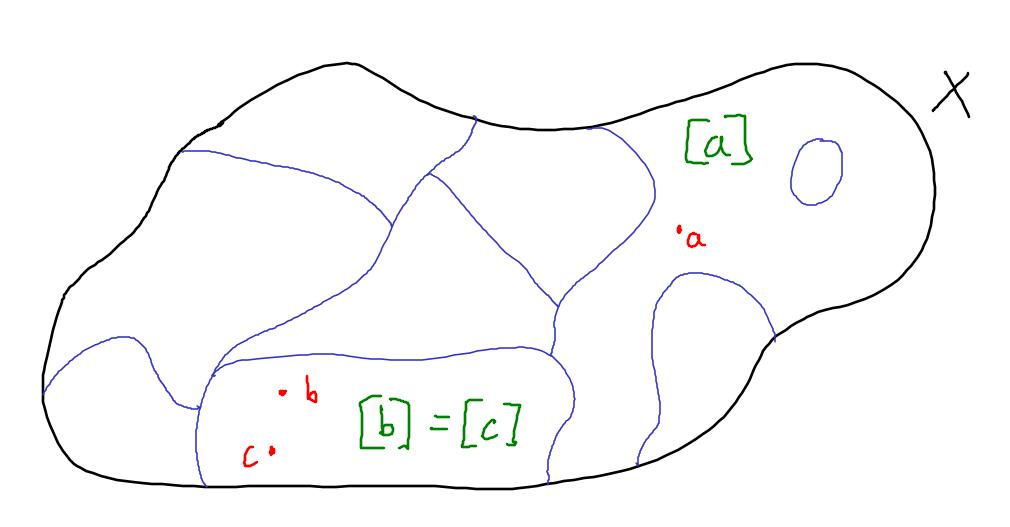
\includegraphics[width=12cm]{./_img/equivalence.jpeg}
	\caption{Die Menge $X$ zerfällt in disjunkte Äquivalenzklassen.}
\end{figure}


% --------------------------------------------------------------------
% §2 Section <<Aufgabenvorschlaege>>
% --------------------------------------------------------------------


\clearpage
\section{Aufgabenvorschläge}





\begin{aufg}[Konkrete Relationen]
Untersuche die folgenden Relationen darauf, ob sie reflexiv, symmetrisch, antisymmetrisch oder transitiv sind. Welche Relationen sind Äquivalenzrelationen, welche Halbordnungen, welche Totalordnungen? Sofern eine Äquivalenzrelation vorliegt, beschreibe die Äquivalenzklassen.
\begin{enumerate}[a)]
\item Es bezeichne $S$ die Menge aller Städte auf der Erde. Betrachte darauf die Relation
\begin{align*}
 A \sim B \quad& :\Leftrightarrow\quad \text{$A$ und $B$ sind höchstens 100km voneinander entfernt} && A,B\in S
\end{align*}
\item Auf der Menge $\Rz$ die Ungleichheitsrelation „$\neq$“.
\item Auf der Menge $\Rz$ die übliche „$<$“-Relation.
\item Es sei $M$ die Menge aller Menschen. Betrachte darauf die Relation
\begin{align*}
 a \sim b \quad& :\Leftrightarrow\quad \text{$a$ und $b$ haben (bzw. hatten) ein gemeinsames Kind} && a,b\in M
\end{align*}
\item Auf der Menge $\Zz$ die Teilbarkeitsrelation
\begin{align*}
 m\mid n \quad& :\Leftrightarrow\quad \exists c\in \Zz:\  c\cdot m=n && m,n \in \Zz
\end{align*}
\end{enumerate}
\end{aufg}


 
 
 
 
 \begin{aufg}[Abstrakte Relationen] \label{abstraktrel}
Untersuche die folgenden Relationen darauf, ob sie reflexiv, symmetrisch, antisymmetrisch oder transitiv sind. Welche Relationen sind Äquivalenzrelationen, welche Halbordnungen, welche Totalordnungen? Sofern eine Äquivalenzrelation vorliegt, beschreibe die Äquivalenzklassen.
\begin{enumerate}[a)]
	\item Auf einer beliebigen Menge $X$ die Gleichheitsrelation „$=$“.
	\item Für zwei Mengen $X,Y$ und eine beliebige Abbildung $f:X\to Y$ die Relation
	\begin{align*}
	 a\sim b \quad &:\Leftrightarrow\quad f(a)=f(b) && a,b\in X
	\end{align*}
          \item Auf einer beliebigen Menge $X$ die „Allrelation“, bezüglich der für alle $x,y\in X$ gilt, dass $x\sim y$. Verkörpert wird diese Relation durch die Teilmenge $X\times X\subseteq X\times X$.
        \item Auf einer beliebigen Menge $X$ die „leere Relation“, bezüglich der gar keine Elemente von $X$ zueinander in Beziehung stehen und die durch die Teilmenge $\emptyset\subseteq X\times X$ verkörpert wird.
\end{enumerate}
 \end{aufg}

 


\begin{aufg}[Graphen]
Bestimme, ob die Relationen, die durch die folgenden Graphen repräsentiert werden, reflexiv, symmetrisch, antisymmetrisch und/oder transitiv sind. Liegt sogar eine Äquivalenzrelation oder eine Ordnungsrelation vor?
\begin{figure}[H]
	\begin{tikzpicture}
		\begin{scope}[xshift=-6cm]
			\node (P0) at (-1,1) {$a$};
			\node (P1) at (-1,-1) {$b$};
			\node (P2) at (1,-1) {$c$};
			\node (P3) at (1,1) {$d$};
			\path[commutative diagrams/.cd, every arrow, every label]
			(P3) edge[commutative diagrams/loop] (P3)
			(P2) edge (P0)
			(P0) edge (P3)
			(P1) edge[<->] (P2);
		\end{scope}
		\begin{scope}[xshift=-2cm]
			\node (P0) at (-1,1) {$a$};
			\node (P1) at (-1,-1) {$b$};
			\node (P2) at (1,-1) {$c$};
			\node (P3) at (1,1) {$d$};
			\path[commutative diagrams/.cd, every arrow, every label]
			(P0) edge (P2)
			(P1) edge (P2)
			(P0) edge[<->] (P1);
		\end{scope}
		\begin{scope}[xshift=2cm]
			\node (P0) at (-1,1) {$a$};
			\node (P1) at (-1,-1) {$b$};
			\node (P2) at (1,-1) {$c$};
			\node (P3) at (1,1) {$d$};
			\path[commutative diagrams/.cd, every arrow, every label]
			(P1) edge[commutative diagrams/loop] (P1)
			(P2) edge[commutative diagrams/loop] (P2)
			(P3) edge[commutative diagrams/loop] (P3)
			(P0) edge[commutative diagrams/loop] (P0)
			(P1) edge[<->] (P2);
		\end{scope}
		\begin{scope}[xshift=6cm]
			\node (P0) at (-1,1) {$a$};
			\node (P1) at (-1,-1) {$b$};
			\node (P2) at (1,-1) {$c$};
			\node (P3) at (1,1) {$d$};
			\path[commutative diagrams/.cd, every arrow, every label]
			(P0) edge (P1)
			(P0) edge (P2)
			(P0) edge (P3)
			(P1) edge (P2)
			(P3) edge (P2);
		\end{scope}
	\end{tikzpicture}
\end{figure}
 \end{aufg}
 




\begin{aufg}[Äquivalenzklassen]
 Betrachte die beiden Abbildungen
 \begin{align*}
   f : \Rz^2 \to \Rz \ &,\ (x,y) \mapsto x+y \\
   g : \Rz^2 \to \Rz \ &,\ (x,y) \mapsto x^2+y^2
 \end{align*}
 Nach \cref{abstraktrel}b) sind durch
 	\begin{align*}
	 p\sim_f q \quad &:\Leftrightarrow\quad f(p)=f(q) && p,q\in \Rz^2 \\
	 p\sim_g q \quad &:\Leftrightarrow\quad g(p)=g(q) && p,q\in \Rz^2
	\end{align*}
zwei Äquivalenzrelationen $\sim_f$, $\sim_g$ auf $\Rz^2$ gegeben. Visualisiere die Äquivalenzklassen jeweils durch eine Zeichnung.
\end{aufg}



 \begin{aufg}[Laptops] \label{laptopaufg}
Zeige, dass auf der Menge $X$ aller Laptops die Relation \glqq\_ ist das gleiche Modell wie \_ \grqq eine Äquivalenzrelation ist. Verdeutliche Dir anhand des Beispiels noch einmal den Unterschied zwischen $X$ und $\sfrac{X}{\sim}$.
\end{aufg}

 
 \begin{comment}
\begin{aufg}[Parallelität]
Eine \textit{Gerade} $g$ in der Ebene $\Rz^2$ ist eine Menge der Form
\[ g= \left\{ x+ty \mid t\in\Rz \right\} \,, \]
wobei $x\in\Rz^2$ ein \textit{Ortsvektor} und $y\in\Rz^2$ ein \textit{Richtungsvektor} der Geraden genannt werden.

Auf der Menge aller Geraden in der Ebene $\Rz^2$ betrachten wir die Relation $g\parallel h :\Leftrightarrow$ $g$ ist parallel zu $h$, oder genauer: ein möglicher Richtungsvektor von $g$ ist ein Vielfaches eines möglichen Richtungsvektors von $h$. Ist etwa
\begin{align*}
	g&=\left\{x+ty\mid t\in\Rz \right\} & y&=\left\{u+tv\mid t\in\Rz\right\}
\end{align*}
für gewisse Vektoren $x,y,u,v\in\Rz^2$, so kannst Du annehmen
\[ g\parallel h \Leftrightarrow \exists r\in\Rz: y=rv \,. \]

Zeige, dass Parallelität auf der Menge aller Geraden in $\Rz^2$ eine Äquivalenzrelation bildet. Was sind die Äquivalenzklassen?
\end{aufg}
\end{comment}


%%% Local Variables:
%%% mode: latex
%%% TeX-master: "Skript"
%%% End:



\setchapterpreamble[c][.7\textwidth]{\itshape\dgrau\small
    Der Begriff der Verknüpfung verallgemeinert die aus der Schule bekannten Rechenoperationen. In diesem Vortrag werden grundlegende Eigenschaften von Verknüpfungen untersucht und ein paar Konsequenzen daraus abgeleitet.
\vspace{24pt}}


\chapter{Verknüpfungen}


\section{Allgemeines}


\begin{de} \index{Verknüpfung}
    Sei $X$ eine beliebige Menge. Eine (zweistellige) \textbf{Verknüpfung auf $X$} ist eine Abbildung $X\times X \to X$, d.h. eine Abbildung, die jedem Elementepaar von $X$ wiederum ein Element von $X$ zuordnet. Eine zweistellige Verknüpfung wird in der Regel mit einem „Verknüpfungszeichen“ notiert. Das heißt: ist der Name der Abbildung etwa „$*$“, so schreibt man
        \[ x*y \qquad\text{anstelle von}\qquad *(x,y) \]
    für den Funktionswert des Paares $(x,y)$ unter der Abbildung $*$.
\end{de}


\begin{bem}[* Verallgemeinerungen]
    Eine zweistellige Verknüpfung auf $X$ ist also eine Art „Automat“, der je zwei Elemente von $X$ entgegennimmt und als Antwort ein drittes Element ausgibt.
    
    Prinzipiell lassen sich auch dreistellige und höherstellige Verknüpfungen definieren. Auch können Verknüpfungen zwischen verschiedenen Mengen existieren. In diesem Vortrag sollen mit „Verknüpfungen“ aber stets (innere) zweistellige Verknüpfungen gemeint sein, wie sie soeben definiert wurden.
\end{bem}


\begin{bsp}[Grundrechenarten]
    Es gilt:
    \begin{enumerate}
        \item Auf $\R$ ist durch die Addition $(x,y)\mapsto x+y$ eine zweistellige Verknüpfung gegeben. Da die Summe zweier rationaler Zahlen ebenfalls rational ist, liefert „$+$“ auch eine Verknüpfung auf der Menge $\Q$. Ebenso ist auch auf $\N$ und $\Z$ durch die Addition „$+$“ jeweils eine Verknüpfung gegeben.
        \item Auf den Mengen $\Z,\Q,\R,\C$ ist durch die Subtraktion $(x,y)\mapsto x-y$ jeweils eine zweistellige Verknüpfung gegeben. Allerdings ergibt der Ausdruck
        \[ \text{„$\N \times \N \to \N \ ,\ (x,y) \mapsto x-y$“} \]
        \emph{keinen} Sinn, da etwa $2-3$ gar kein Element von $\N$ ist. Auf $\N$ ist die Subtraktion also \textbf{keine} zweistellige Verknüpfung. Zwar lassen sich für gewisse Zahlenpaare durchaus Differenzen in $\N$ bilden (z.B. $3-2$); dass $-$ eine Verknüpfung auf $\N$ wäre, scheitert aber daran, dass eben nicht \emph{jedes} Paar natürlicher Zahlen eine Differenz in $\N$ besitzt.
        \item Auf den Mengen $\N,\Z,\Q,\R,\C$ ist durch die Multiplikation $(x,y)\mapsto x\cdot y$ jeweils eine zweistellige Verknüpfung gegeben.
        \item Auf den Mengen $\Q\setminus \{0\},\R\setminus \{0\},\C\setminus \{0\}$ ist durch die Division $(x,y)\mapsto x:y$ jeweils eine zweistellige Verknüpfung gegeben. Beachte, dass die Null ausgelassen werden muss, weil bspw. nicht „$1:0$“ gebildet werden kann. Zwar könnte man $1:0=\infty$ setzen, aber $\infty$ wäre kein Element von $\Q,\R$ bzw. $\C$, sodass dadurch nachwievor keine Verknüpfung auf $\Q,\R$ bzw. $\C$ zustandekäme.
    \end{enumerate}
\end{bsp}


\begin{bsp}[Verketten von Abbildungen]
    Sei $M$ eine beliebige Menge. Dann ist auf der Menge $\Abb(M,M)$ der Selbstabbildungen von $M$ eine Verknüpfung gegeben durch die Verkettung\footnote{siehe \cref{def:verkettung}} von Abbildungen:
        \[ \Abb(M,M)\times \Abb(M,M)\to \Abb(M,M) \ ,\ (f,g)\mapsto f\circ g \]
\end{bsp}


\begin{bem}[*]
    Beachte, dass in diesem Beispiel von Selbstabbildungen (also Abbildungen, deren Definitions- und Wertebereich übereinstimmen) die Rede ist. Sind allgemein $A,B,C$ drei Mengen, so hat man zwar eine Abbildung
        \[ \Abb(B,C) \times \Abb(A,B) \to \Abb(A,C) \ ,\ (f,g) \mapsto f\circ g \]
    sofern $A,B,C$ drei verschiedene Mengen sind, ist dies aber \textbf{keine} zweistellige Verknüpfung -- denn auf welcher Menge sollte diese Verknüpfung „leben“, wenn ja $\Abb(B,C)$ und $\Abb(A,B)$ zwei verschiedene Mengen sind?
    
    Nichtsdestotrotz besitzt auch das allgemeine Verketten von Abbildungen die interessante, häufig auftretende Struktur einer sogenannten \href{https://ncatlab.org/nlab/show/category}{Kategorie}. Mehr darüber wirst du spätestens in fortgeschrittenen Algebra-Vorlesungen erfahren.
\end{bem}


\begin{bsp}[Operationen mit Mengen]
    Sei $M$ eine beliebige Menge. Auf der Potenzmenge $\calP(M)$ haben wir beispielsweise folgende Verknüpfungen:
    \begin{align*}
        \cap : \calP(M)\times \calP(M) \to \calP(M) \ & ,\ (A,B)\mapsto A\cap B \\
        \cup : \calP(M)\times \calP(M) \to \calP(M) \ &,\ (A,B)\mapsto A\cup B \\
        \setminus : \calP(M)\times \calP(M) \to \calP(M) \ &,\ (A,B)\mapsto A\setminus B
    \end{align*}
    Denn der Durchschnitt / die Vereinigung / die Differenzmenge zweier Teilmengen von $M$ ist ebenfalls eine Teilmenge von $M$.
\end{bsp}


\begin{bsp}[* Kleineres und Größeres zweier Elemente] \label{bsp:minmaxverknuepfung}
    Auf $\R$ gibt es die beiden Verknüpfungen
    \begin{align*}
        \min : \R\times \R\to \R\ &,\ (x,y)\mapsto \min\{x,y\} \\
        \max : \R\times \R\to \R\ &,\ (x,y)\mapsto \max\{x,y\}
    \end{align*}
    die ein Zahlenpaar jeweils auf die kleinere bzw. die größere der beiden Zahlen abbildet. Eine Verallgemeinerung sowohl dieses Beispiels als auch des Beispiels mit $\cap$ und $\cup$ stellen sogenannte \href{https://de.wikipedia.org/wiki/Verband_(Mathematik)}{Verbände} dar.
\end{bsp}


\begin{bem}
    Alle bisher beschriebenen Verknüpfungen besaßen ein spezifisches eigenes Verknüpfungssymbol und waren relativ übersichtlich aufzuschreiben. Allgemeine Verknüpfungen auf einer Menge $X$ dürfen aber beliebig kompliziert sein. Es muss sich ja lediglich um \emph{irgendeine} Abbildung $X\times X\to X$ handeln, die beliebig chaotisch sein darf und keinem Muster gehorchen muss. Neben Addition und Multiplikation gibt es auf $\N$ unendlich viele weitere Verknüpfungen, von denen die meisten wohl niemals von mathematischem Interesse sein werden.
\end{bem}


\begin{nota}[Verknüpfungssymbole]
    In diesem Text werden wir, wenn wir über eine „allgemeine zweistellige Verknüpfung“ schreiben, die Verknüpfung mit einem „$*$“ notieren. Die vorigen Beispiele zeigen, dass konkrete Verknüpfungen auch mit ganz anderen Zeichen wie etwa $+,-,\cdot,:,\cap,\cup$ usw. notiert werden. Andere Bücher und Vorlesungen verwenden auch andere Symbole wie etwa „$\odot$“ oder „$\circ$“, um über „die allgemeine Verknüpfung“ zu reden.
\end{nota}





\section{Assoziativ- und Kommutativgesetz}


\begin{de} \index{assoziative Verknüpfung} \index{kommutative Verknüpfung}
    Seien $X$ eine Menge und $*$ eine Verknüpfung auf $X$. Die Verknüpfung $*$ heißt
    \begin{itemize}
        \item \textbf{assoziativ}, falls für alle $x,y,z\in X$ das sogenannte \emph{Assoziativgesetz} gilt:
            \[ x*(y*z) = (x*y)*z \]
        \item \textbf{kommutativ}, falls für alle $x,y\in X$ das sogenannte \emph{Kommutativgesetz} gilt:
            \[ x*y = y*x \]
    \end{itemize}
\end{de}


\begin{bsp}
    Es gilt:
    \begin{enumerate}
        \item Auf $\N,\Z,\Q,\R,\C$ sind die Addition $+$ und die Multiplikation $\cdot$ sowohl assoziativ als auch kommutativ. Denn für alle natürlichen/ganzen/rationalen/reellen/komplexen Zahlen $x,y,z$ gilt bekanntlich
        \begin{align*}
            x+(y+z)& = (x+y)+z  \\
            x+y & = y+x \\
            x\cdot (y\cdot z) & = (x\cdot y)\cdot z  \\
            x\cdot y & = y\cdot x
        \end{align*}
        \item Die Subtraktion auf $\Z,\Q,\R,\C$ ist weder assoziativ noch kommutativ. Beispielsweise ist
        \begin{align*}
            3-(2-1) &\neq  (3-2)-1  \\
            3-2 &\neq 2-3
        \end{align*}
        \item Die Division auf $\Q\setminus \{0\},\R\setminus \{0\},\C\setminus \{0\}$ ist weder assoziativ noch kommutativ. Beispielsweise ist
        \begin{align*}
            2:(3:2) = 4:3 &\neq 1:3 = (2:3):2 \\
            2 : 3 & \neq 3:2
        \end{align*}
        \item Für jede Menge $M$ ist das Verketten von Abbildungen eine assoziative Verknüpfung auf $\Abb(M,M)$. Dies wurde in \cref{abbassoziativ} bewiesen. Im Allgemeinen (nämlich sobald $M$ mindestens zwei verschiedene Elemente enthält) ist sie aber nicht kommutativ, vgl. \cref{bsp:verkettung}.
        \item Ist $M$ eine beliebige Menge, so sind die beiden Verknüpfungen $\cap$ und $\cup$ auf $\calP(M)$ sowohl assoziativ als auch kommutativ, siehe \cref{aufg:capcupgesetze} Die Operation $\setminus$ ist aber, sofern $M$ nichtleer ist, weder assoziativ noch kommutativ.
    \end{enumerate}
\end{bsp}


\begin{bsp}[* Rechnen mit Rundungsfehlern] \label{bsp:fehlerrech}
    So gut wie alle Verknüpfungen in den ersten Semestern Mathematikstudium sind assoziativ. Ein für die Informatik wichtiges Beispiel für eine nicht-assoziative Verknüpfung ist die „fehlerbehaftete Multiplikation“. Da ein Computer eine Zahl nicht mit beliebig vielen Nachkommastellen speichern kann, muss er nach solchen Rechenschritten, die die Anzahl der Nachkommastellen übers Maximum erhöhen würde, die letzte verfügbare Nachkommastelle runden. Für ein vereinfachtes Beispiel betrachte die Menge
        \[ \frac{1}{10}\Z := \left\{ x\in \Q \mid \exists n\in \Z:\ x=\frac{n}{10} \right\} \]
    all derjenigen rationalen Zahlen, die höchstens eine Nachkommastelle im Dezimalsystem besitzen (Computer würden im Binärsystem rechnen und erheblich mehr Nachkommastellen einbeziehen). Auf dieser Menge ist folgendermaßen eine zweistellige Verknüpfung „$*$“ gegeben:
    \begin{quote}
        Für $a,b\in \frac{1}{10}\Z$ bilde zuerst das gewöhnliche Produkt rationaler Zahlen $a\cdot b \in \Q$. Runde dieses Produkt nun auf die erste Nachkommastelle. Diese gerundete Zahl sei $a*b$.
    \end{quote}
    Für diese Verknüpfung gilt beispielsweise:
    \begin{align*}
        1{,}5* 0{,}5 = 0{,}8 \qquad 0{,}1* 0{,}1 = 0 \qquad 2*3 = 6 \qquad 1{,}5 * (-0{,}3)= -0{,}5 
    \end{align*}
    Diese „ungenaue Multiplikation“ ist zwar kommutativ, aber nicht assoziativ, da beispielsweise:
    \begin{align*}
        (0{,}1 * 0{,}1) * 10 & = 0*10 = 0 \\
        0{,}1*(0{,}1*10) & = 0{,}1*1 = 0{,}1
    \end{align*}
\end{bsp}


\begin{bem}[Die eigentliche Bedeutung der Assoziativität] \label{klammerfrei}
    Sei $X$ eine Menge mit einer assoziativen Verknüpfung $*$. Der Grund dafür, dass das Assoziativgesetz so eine wichtige Rolle spielt, ist, dass bei einer assoziativen Verknüpfung keine Klammern gesetzt werden müssen. Das Assoziativgesetz selbst
    \begin{align*}
        (x*y)*z = x*(y*z) && x,y,z\in X
    \end{align*}
    besagt schonmal, dass bei solchen Termen, die nur drei Elemente involvieren, jede Art von Klammernplatzierung auf dasselbe Ergebnis hinausläuft. Daher schreibt man einfach
        \[ x*y*z \]
    Mit fortgeschrittenen Techniken lässt sich beweisen, dass bei assoziativen Verknüpfungen sogar in Termen mit beliebig vielen Elementen jede Art von Klammerung auf dasselbe Ergebnis hinausläuft. Beispielsweise gilt für $a,b,c,d,e\in X$:
    \begin{align*}
        (a*(b*c))*(d*e) & =((a*b)*c)*(d*e) && (\text{Assoziativität für $a$, $b$ und $c$})\\
        & = (((a*b)*c)*d)*e && (\text{Assoziativität für $(a*b)*c$, $d$ und $e$})  \\
        & = ((a*b)*(c*d))*e && (\text{Assoziativität für $a*b$, $c$ und $d$})\\
        &=\ \text{usw.}
    \end{align*}
    Daher können bei assoziativen Verknüpfungen ganz allgemein überall die Klammern weglassen werden; in diesem Fall schriebe man schlicht
        \[ a*b*c*d*e \]
    Aus der Schule bist du es ja auch gewohnt, einfach
        \[ 1+3+2+4 \qquad\text{anstelle von}\qquad (1+3)+(2+4)\ \text{oder}\ (1+(3+2))+4 \]
    zu schreiben und daran ändert sich auch an der Uni nichts. Sind beispielsweise $A,B,C,D$ vier Mengen, so schreibt man schlicht
        \[ A\cup B\cup C \cup D \]
    für deren Vereinigung, was unproblematisch ist, da $\cup$ eine assoziative Verknüpfung ist. Sind $\begin{tikzcd}[cramped] A\ar[r, "f"] & B\ar[r, "g"] & C \ar[r, "h"] & D \end{tikzcd}$ drei Abbildungen, so schreibt man
        \[ h\circ g\circ f \]
    für deren Verkettung, wobei auch hier wegen der Assoziativität keine Klammern gesetzt werden müssen.\footnote{vgl. \cref{abbklammerfrei}}
\end{bem}




 
\section{Monoide}


\begin{de}[Neutrales Element] \label{def:neutrales} \index{neutrales Element}
    Seien $X$ eine Menge und $*$ eine zweistellige Verknüpfung auf $X$. Ein Element $e\in X$ heißt \textbf{neutrales Element}, falls für jedes $x\in X$ die folgenden beiden Gleichungen gelten:
    \begin{align*}
        e*x & = x && (\text{Linksneutralität}) \\
        x*e & = x && (\text{Rechtsneutralität})
    \end{align*}
\end{de}


\begin{bsp} \label{bsp:neutrales}
    Mit einer beliebigen Menge $M$ gilt:
    \begin{enumerate}
        \item Die Addition auf $\R$ hat die Zahl Null als neutrales Element. Denn für jede reelle Zahl $x\in \R$ gilt ja
            \[ 0+x=x \qquad\text{und}\qquad x+0=x \]
        Ebenso ist die Null auch neutrales Element zur Addition auf $\N,\Z,\Q$ und $\C$.
        \item Die Multiplikation auf $\R$ hat die Zahl Eins als neutrales Element. Denn für jede reelle Zahl $x\in \R$ ist
            \[ 1\cdot x = x\cdot 1= x \]
        Ebenso ist die Eins auch neutrales Element zur Multiplikation auf $\N,\Z,\Q$ und $\C$.
        \item Das Verketten von Abbildungen aus $\Abb(M,M)$ hat die Identität $\id_M$ als neutrales Element. Denn in \cref{idneutral} wurde bewiesen, dass für jede Abbildung $M\xrightarrow{f} M$ gilt:
            \[ f\circ \id_M = f \qquad\text{und}\qquad \id_M \circ f = f \]
        \item Bezüglich der Verknüpfung $\cap$ hat $\calP(M)$ das neutrale Element $M$. Denn es gilt:
        \begin{align*}
            M\cap A & = A\cap M = A && \text{für jede Teilmenge}\ A\subseteq M
        \end{align*}
        \item Bezüglich der Verknüpfung $\cup$ hat $\calP(M)$ das neutrale Element $\emptyset$. Denn es gilt:
        \begin{align*}
            \emptyset\cup A & = A\cup \emptyset = A && \text{für jede Teilmenge}\ A\subseteq M
        \end{align*}
        \item Die fehlerbehaftete Multiplikation aus \cref{bsp:fehlerrech} hat die $1$ als neutrales Element. Denn wenn ich eine rationale Zahl, die höchstens eine Nachkommastelle besitzt, mit $1$ multipliziere, ändert sich nichts, sodass auch das nachfolgende Runden nichts am Zahlenwert ändert.
        \item Hinsichtlich der Subtraktion auf $\Z,\Q,\R$ bzw. $\C$ gibt es \emph{kein} neutrales Element. Denn wäre $e$ ein solches Element, so gälte
            \[ 0-4 = (e-0)-4 = e-4 = 4 \]
        was nicht sein kann.
        \item Hinsichtlich der Division auf $\Q\setminus \{0\},\R\setminus \{0\},\C\setminus \{0\}$ gibt es ebenfalls kein neutrales Element.
    \end{enumerate}
\end{bsp}


\begin{bem}[Beweisarbeit einsparen im kommutativen Fall]
    Seien $X$ eine Menge mit einer Verknüpfung $*$ und $e\in X$ ein Element, von dem du vermutest, dass es ein neutrales Element ist. Sofern $*$ eine \emph{kommutative Verknüpfung} ist, brauchst du, um zu beweisen, dass $e$ ein neutrales Element ist, von den beiden Gleichungen
        \[ e*x=x \qquad\text{und}\qquad x*e=x \qquad\qquad x\in X \]
    nur eine zu beweisen. Die andere folgt dann direkt aus dem Kommutativgesetz.
\end{bem}


\begin{satz}[Eindeutigkeit neutraler Elemente] \label{neutreind}
    Seien $X$ eine Menge und $*$ eine Verknüpfung auf $X$. Sofern $X$ diesbezüglich ein neutrales Element enthält, ist dieses eindeutig bestimmt.
\end{satz}
 

\begin{bew}
    Es seien $e,d\in X$ zwei neutrale Elemente bezüglich der Verknüpfung $*$. Dann gilt:
    \begin{align*}
        d & = d*e && (\text{weil $e$ neutrales Element}) \\
        & = e && (\text{weil $d$ neutrales Element}) && \qed
    \end{align*}
\end{bew}


\begin{bem}[\textbf{Das} neutrale Element]
    Der Eindeutigkeitssatz berechtigt uns, beim Vorhandensein eines neutralen Elements statt von „einem neutralen Element“ von \emph{dem} neutralen Element zu reden.
    
    An diesem Satz wird vielleicht deutlich, wie vorteilhaft die axiomatische Arbeit mit abstrakten Verknüpfungen sein kann. Denn er garantiert uns auf einen Schlag, dass die neutralen Elemente aus allen Beispielen in \cref{bsp:neutrales} auch jeweils die einzigen neutralen Elemente sind, ohne dass wir dies in jedem Fall einzeln beweisen müssten.
\end{bem}


\begin{de}[Monoid] \index{Monoid}
    Ein \textbf{Monoid} ist ein Paar $(M,*)$ bestehend aus einer Menge $M$ und einer Verknüpfung $*$ auf $M$, für das gilt:
    \begin{enumerate}[(M1), labelindent=1.5em, leftmargin=*]
        \item $*$ ist eine assoziative Verknüpfung.
        \item $M$ enthält ein neutrales Element (bezüglich der Verknüpfung $*$).
    \end{enumerate}
    In diesem Fall ist das neutrale Element nach \cref{neutreind} automatisch eindeutig bestimmt.
    
    Ist überdies die Verknüpfung $*$ auch noch kommutativ, so heißt $(M,*)$ ein \textbf{kommutatives Monoid}.
\end{de}


\begin{bsp} Es gilt:
    \begin{enumerate}
        \item $(\N_0,+),(\Z,+),(\Q,+),(\R,+),(\C,+)$ sind jeweils kommutative Monoide. Denn die Addition ist assoziativ und kommutativ und die Zahl $0$ ist ihr neutrales Element.
        \item $(\N,\cdot),(\Z,\cdot),(\Q,\cdot),(\R,\cdot),(\C,\cdot)$ sind jeweils kommutative Monoide. Denn die Multiplikation ist assoziativ und kommutativ und die Zahl $1$ ist ihr neutrales Element.
        \item Die Subtraktion und die Division liefern keine Monoide, weil sie nicht assoziativ sind. Und ein neutrales Element besitzen sie ja auch nicht.
        \item Ist $M$ eine beliebige Menge, so ist $(\Abb(M,M),\circ)$ ein Monoid mit neutralem Element $\id_M$. Sofern $M$ mindestens zwei verschiedene Elemente enthält, ist es aber nicht kommutativ.
        \item Ist $M$ eine beliebige Menge, so sind $(\calP(M),\cup)$ und $(\calP(M),\cap)$ zwei kommutative Monoide mit den jeweiligen neutralen Elementen $\emptyset$ und $M$.
        \item Die „fehlerbehaftete Multiplikation“ aus \cref{bsp:fehlerrech} besitzt zwar ein neutrales Element -- sie liefert aber kein Monoid, weil sie nicht assoziativ ist.
        \item Die Addition „$+$“ ist zwar eine assoziative Verknüpfung auf der Menge $\N_{\ge 1}$, aber $(\N_{\ge 1},+)$ ist kein Monoid, da es kein neutrales Element enthält.
    \end{enumerate}
\end{bsp}


\begin{bem}[Trägermenge]
    Beachte, dass ein Monoid immer ein Paar $(M,*)$ ist, in das sowohl die „Trägermenge“ $M$ als auch die Verknüpfung $*$ hineinkodiert ist. Ein und dieselbe Menge kann durchaus als Trägermenge für verschiedene Monoide herhalten. Beispielsweise sind $(\N_0,+)$ und $(\N_0,\cdot)$ zwei verschiedene Monoide, die dennoch dieselbe Trägermenge $\N_0$ besitzen.
    
    Andererseits gibt es Mengen mit „kanonischen“ Verknüpfungen, wie z.B. $\Abb(X,X)$ (wobei $X$ irgendeine Menge ist). Sprechen Mathematiker von „dem Monoid $\Abb(X,X)$“, so meinen sie damit grundsätzlich das Monoid $(\Abb(X,X),\circ)$, also $\Abb(X,X)$ mit der Verkettung von Abbildungen als Verknüpfung. Solche Konventionen wirst du mit der Zeit durch Erfahrung und Gewohnheit verinnerlichen.
    
    Ist im Kontext klar oder gleichgültig, von welcher Verknüpfung die Rede ist, so spricht man abkürzend meist nur von „dem Monoid $M$“.
\end{bem}


\begin{bem}[Die eigentliche Bedeutung des Kommutativgesetzes]
    Es sei $(M,*)$ ein kommutatives Monoid. Weil dann $*$ assoziativ ist, brauchen wir nach \cref{klammerfrei} keine Klammern setzen. Sind beispielsweise $a,b,c,d\in M$, so können wir einfach
        \[ a*b*c*d \]
    schreiben. Das Kommutativgesetz
    \begin{align*}
        x*y&=y*x && \text{für alle}\ x,y\in M
    \end{align*}
    sagt nun aus, dass es bei der Verknüpfung \emph{zweier} Elemente nicht auf die Reihenfolge ankommt. Es lässt sich zeigen, dass es damit sogar bei der Verknüpfung beliebig vieler Elemente nicht auf die Reihenfolge ankommt. Beispielsweise gilt
    \begin{align*}
        a*b*c*d & = a*c*b*d && (\text{Kommutativgesetz für $b$ und $c$}) \\
        & = c*a*b*d && (\text{Kommutativgesetz für $a$ und $c$}) \\
        & = b*d*c*a && (\text{Kommutativgesetz für $c*a$ und $b*d$}) \\
        & \text{usw.}
    \end{align*}
    Bei kommutativen Monoiden brauchst du also weder aufs Klammernsetzen, noch auf die Reihenfolge, in der du die Elemente verknüpfst, achten.
\end{bem}


\begin{de}[Inverse Elemente] \label{def:inverse} \index{inverses Element} \index{Einheit (bei einer Verknüpfung)}
    Sei $X$ eine Menge mit einer zweistelligen Verknüpfung $*$, die ein (nach \cref{neutreind} automatisch eindeutig bestimmtes) neutrales Element $e$ besitzt. Ein Element $b\in M$ heißt \textbf{invers} zu $a$, falls es die folgenden beiden „Inversengleichungen“ erfüllt:
    \begin{align*}
        a*b & = e && (\text{„$b$ ist rechtsinvers zu $a$“}) \\
        b*a & = e && (\text{„$b$ ist linksinvers zu $a$“})
    \end{align*}
    Das Element $a$ heißt \textbf{invertierbar} (oder auch: \emph{Einheit}\footnote{Die Analogie zum Einheitenbegriff aus der Physik (z.B. „Meter“ und „Kilogramm“) besteht darin, dass in einem Monoid in einem gewissen Sinn jedes Element ein „Vielfaches“ jeder Einheit ist, so wie jede Länge als Vielfache der Einheit „Meter“ angegeben werden kann.}), falls es ein zu $a$ inverses Element in $X$ gibt.
\end{de}


\begin{bem}[Keine Inversen ohne Neutrales]
    Beachte, dass es nur bei Vorhandensein eines neutralen Elements überhaupt Sinn ergibt, von inversen Elementen zu sprechen. 
\end{bem}


\begin{bsp} \label{bsp:inverse}
    Es gilt:
    \begin{enumerate}
        \item In den Monoiden $(\Z,+),(\Q,+),(\R,+),(\C,+)$ ist jedes Element invertierbar. Denn für jede ganze/rationale/reelle/komplexe Zahl $x$ gilt
        \begin{align*}
            x + (-x) & = 0 \\
            (-x) + x & = 0
        \end{align*}
        sodass $-x$ invers zu $x$ ist.
        \item Das einzige invertierbare Element im Monoid $(\N_0,+)$ ist die $0$, da $0+0=0$. Für jede andere Zahl $n\in \N_{\ge 1}$ kann es kein $m\in \N_0$ mit $n+m=0$ geben.
        \item In den Monoiden $(\Q,\cdot),(\R,\cdot),(\C,\cdot)$ ist jedes Element $\neq 0$ invertierbar. Denn für jede rationale/reelle/komplexe Zahl $x\neq 0$ gilt
        \begin{align*}
            x \cdot \frac{1}{x} & = 1 \\
            \frac{1}{x}\cdot x & = 1
        \end{align*}
        sodass $\frac{1}{x}$ invers zu $x$ ist. Die Null ist dagegen nicht invertierbar. Denn für jede beliebige Zahl $x$ ist $0\cdot x = 0\neq 1$, sodass $x$ nicht invers zur $0$ sein kann.
    \end{enumerate}
\end{bsp}

    
\begin{bem}[Beweisarbeit einsparen im kommutativen Fall]
    Sei $X$ eine Menge mit einer Verknüpfung $*$, die ein neutrales Element $e\in X$ besitzt. Außerdem seien $a,b\in X$ und du vermutest, dass $b$ invers zu $a$ ist. Sofern $*$ eine \emph{kommutative} Verknüpfung ist, brauchst du, um zu beweisen, dass $b$ invers zu $a$ ist, von den beiden Gleichungen
        \[ a*b=e\qquad\text{und}\qquad b*a=e \]
    nur eine zu beweisen. Die andere folgt dann aus dem Kommutativgesetz.
\end{bem}


\begin{bsp}[*]
    Das folgende Beispiel zeigt, dass im Allgemeinen nicht aus der Gültigkeit einer der beiden Inversengleichungen schon auf die andere geschlossen werden kann.
    
    Betrachte das Monoid $\Abb(\N_0,\N_0)$ und darin die beiden Abbildungen
    \begin{align*}
        f : \N_0 \to \N_0 \ &,\ n \mapsto n+1 \\
        g: \N_0 \to \N_0 \ &,\ n\mapsto \begin{cases}
            0 & n=0 \\
            n-1 & n\ge 1
        \end{cases}
    \end{align*}
    Dann gilt zwar $g\circ f=\id_{\N_0}$. Allerdings ist $f\circ g\neq \id_{\N_0}$, sodass $g$ nicht invers zu $f$ ist. Tatsächlich kann $f$ gar keine Inverse besitzen, da $f$ wegen $0\notin \im(f)$ nicht surjektiv, also erst recht nicht bijektiv, ist.
\end{bsp}


\begin{satz}[Eindeutig inverser Elemente] \label{inveind}
    Seien $(M,*)$ ein Monoid und $a\in M$ ein invertierbares Element. Dann ist das inverse Element von $a$ eindeutig bestimmt.\footnote{vgl. \cref{umkehreind}}
\end{satz}
 
 
\begin{bew}
    Es seien $e\in M$ das neutrale Element von $M$ und $b,c\in M$ zwei beliebige Inverse zu $a$. Dann gilt:
    \begin{align*}
        b & = b*e && (\text{da $e$ neutral ist}) \\
        & = b* a*c && (\text{da $c$ invers zu $a$ ist}) \\
        & = e*c && (\text{da $b$ invers zu $a$ ist}) \\
        & = c && (\text{da $e$ neutral ist}) &\qed
    \end{align*}
\end{bew}


\begin{nota}[\textbf{Das} inverse Element]
    Seien $(M,*)$ ein Monoid und $a\in M$ ein invertierbares Element. Da dann $a$ auch nur genau ein Inverses besitzt, ergibt es Sinn, anstelle von „einem Inversen zu $a$“ von \emph{dem} Inversen von $a$ zu sprechen. Im Folgenden werde ich das Inverse eines invertierbaren Monoidelements $a$ mit „$a^\inv$“ notieren:
    \begin{align*}
         a^\inv := (\text{Das Inverse von $a$}) && (\text{sofern $a$ invertierbar ist})
    \end{align*}
    Diese Schreibweise ist allerdings unüblich, stattdessen wird meist die Notation „$a^{-1}$“ verwendet, siehe \cref{def:potenz}.
\end{nota}


\begin{bem}[*]
    Beachte, dass ich im Beweis von \cref{inveind} implizit Gebrauch vom Assoziativgesetz gemacht habe (erkennst du, wo?). Bei einer nicht-assoziativen Verknüpfung wie z.B. der fehlerbehafteten Multiplikation aus \cref{bsp:fehlerrech}, die sowohl kommutativ ist als auch ein neutrales Element besitzt, brauchen Inverse nicht eindeutig sein. Beispielsweise gilt dort
    \begin{align*}
        0{,}4 * 2{,}5 & = 1 \\
        0{,}4 * 2{,}6 & = 1
    \end{align*}
    sodass das Element $0{,}4$ mindestens zwei verschiedene Inverse besitzt, nämlich $2{,}5$ und $2{,}6$.
\end{bem}


\begin{satz}[Rechenregeln für inverse Elemente] \label{regelnfuerinv} \index{Involution}
    Sei $(M,*)$ ein Monoid mit neutralem Element $e\in M$. Dann gilt:
    \begin{enumerate}
        \item Das neutrale Element ist invertierbar und es gilt $e^\inv = e$.\footnote{Elemente, die invers zu sich selbst sind, heißen \textbf{selbstinvers} oder auch \textbf{Involutionen}.}
        \item(Inverses vom Inversen) Ist $a\in M$ ein invertierbares Element, so ist auch $a^\inv$ invertierbar und es ist
            \[(a^\inv)^\inv = a \]
        \item(Regel von Hemd und Jacke) Sind $a,b\in M$ zwei invertierbare Element, so ist auch $a*b$ invertierbar und es gilt:
            \[ (a*b)^\inv = b^\inv * a^\inv \]
    \end{enumerate}
\end{satz}


\begin{bew}
    \begin{enumerate}
        \item Da $e$ ein neutrales Element ist, gilt $e*e=e$. Diese Gleichung entspricht beiden Inversengleichungen aus \cref{def:inverse} zugleich.
        \item Da $a^\inv$ invers zu $a$ ist, gelten die beiden Gleichungen
            \[ a*a^\inv = e \qquad\text{und}\qquad a^\inv * a=e \]
        Die erste dieser Gleichungen besagt, dass $a$ linksinvers zu $a^\inv$ ist und die zweite Gleichung besagt, dass $a$ rechtsinvers zu $a^\inv$ ist. Insgesamt ist also $a$ invers zu $a^\inv$.
        \item Es gilt
        \begin{align*}
            \begin{split}
                a*b* b^\inv *a^\inv  & =  a*e*a^\inv \\
                & = a*a^\inv \\
                & = e
            \end{split} & \text{sowie}\qquad \begin{split}
                b^\inv *a^\inv * a*b  & =  b^\inv * e* b \\
                & = b^\inv * b \\
                & = e
            \end{split}
        \end{align*}
        Insgesamt erfüllt $b^\inv *a^\inv$ somit beide Inversengleichungen. \qed
    \end{enumerate}
\end{bew}


\begin{bem} \index{Regel von Hemd und Jacke}
    Die letzte Aussage heißt „Regel von Hemd und Jacke“ aufgrund folgender Analogie: Habe ich mir erst ein Hemd und daraufhin eine Jacke angezogen und möchte ich mich nun wieder entkleiden, so muss ich zuerst die Jacke und dann das Hemd ausziehen. -- Beim Invertieren dreht sich die Reihenfolge um.
\end{bem}





\section{Mehr Notation}


\begin{nota}[additive und multiplikative Notation]
    Zur Notation von Verknüpfungen gibt es zwei häufig vorkommende Schemata:
    \begin{itemize}
        \item Eine \textbf{additiv geschriebene Verknüpfung} ist eine Verknüpfung, die mit dem Zeichen „$+$“ notiert wird. Im Ausdruck
            \[ a + b\]
        heißen $a,b$ die \textbf{Summanden} und $a+b$ die \textbf{Summe}.
        
        In der Algebra herrscht die Konvention vor, \emph{ausschließlich kommutative Verknüpfungen additiv zu schreiben}. Wenn du eine Verknüpfung mit $+$ notierst, werden deine Leser davon ausgehen, dass die Verknüpfung kommutativ sein soll. Daher solltest du nichtkommutative Verknüpungen möglichst nie additiv notieren.
        \item Eine \textbf{multiplikativ geschriebene Verknüpfung} ist eine Verknüpfung, die mit dem Malpunkt „$\cdot$“ notiert wird. Im Ausdruck
            \[ a\cdot b \]
        heißen $a,b$ die \textbf{Faktoren} und $a\cdot b$ das \textbf{Produkt}. Oftmals wird in diesem Fall auch gar kein Verknüpfungssymbol aufgeschrieben: man schreibt dann „$ab$“ anstelle von „$a\cdot b$“, so wie du es aus der Schule von der Multiplikation zweier Zahlvariablen kennst.
    \end{itemize}
    „Additiv geschrieben“ und „multiplikativ geschrieben“ sind keine mathematischen Eigenschaften einer Verknüpfung, sondern nur Fälle von Notation. Prinzipiell könntest du jede Verknüpfung additiv oder multiplikativ schreiben.
\end{nota}


\begin{bsp}
    Additiv geschriebene Verknüpfungen, die dir im ersten Semester begegnen werden, sind neben der Addition von Zahlen die Addition von Polynomen, Vektoren, Matrizen, Folgen und reellwertigen Funktionen.
    
    Multiplikativ geschriebene Verknüpfungen im ersten Semester sind neben der Multiplikation von Zahlen die Multiplikation von Polynomen, Matrizen, Folgen und reellwertigen Funktionen.
\end{bsp}


\begin{nota}[Null- und Einselement] \index{Nullelement} \index{Einselement}
    Sei $X$ eine beliebige Menge. Ist $+$ eine additiv geschriebene Verknüpfung auf $X$, die ein neutrales Element enthält, so wird dieses in der Regel mit „$0$“ notiert und das \textbf{Nullelement} von $X$ genannt. Per Definition gilt
    \begin{align*}
        0 + x = x \qquad\text{und}\qquad x+0= x && \text{für alle}\ x\in X
    \end{align*}
    Ist dagegen „$\cdot$“ eine multiplikativ geschriebene Verknüpfung auf $X$, die ein neutrales Element enthält, so wird dieses oft mit „$1$“ notiert und das \textbf{Einselement} von $X$ genannt. Per Definition gilt
    \begin{align*}
        1 \cdot x = x \qquad\text{und}\qquad x\cdot 1= x && \text{für alle}\ x\in X
    \end{align*}
    Um zu betonen, dass es sich um das Null- bzw. Einselement von $X$ und nicht etwa um die natürliche Zahl Null bzw. Eins handelt, schreibt man auch
    \[ 0_X \qquad\text{bzw.}\qquad 1_X \]
    Beachte, dass Null- und Einselemente im Allgemeinen nichts mit den herkömmlichen Zahlen Null und Eins zu tun haben müssen! Wir bedienen uns lediglich derselben Notation.
\end{nota}


\begin{nota}[Differenzen] \label{differenz}
    Seien $(M,+)$ ein additiv geschriebenes kommutatives Monoid und $a\in M$ ein invertierbares Element. Das Inverse von $a$ wird dann notiert durch
    \begin{align*}
        -a & := a^\inv && (\text{bei einer additiv geschriebenen Verknüpfung})
    \end{align*}
    Für ein weiteres Element $b\in M$ schreibt man
        \[ b-a \qquad\text{anstelle von}\qquad b + (-a) \]
    und spricht von der \textbf{Differenz} von $b$ und $a$. Die Inversengleichungen nehmen mit dieser Notation die folgende Gestalt an:
        \[ a-a = 0 \qquad\text{und}\qquad -a+a = 0 \]
    wobei die zweite Gleichung redundant ist, weil $+$ als kommutativ vorausgesetzt wurde.
    
    Bei Termen mit Summen und Differenzen mehrerer Elemente $a_1,\dots , a_n\in M$ lässt man die Klammern in der Regel weg unter der stillschweigenden Voraussetzung, die Terme als „linksassoziativ“ zu interpretieren:
        \[ a_1 \pm a_2\pm a_3\pm\ldots\pm a_n := (((a_1\pm a_2)\pm a_3) \pm \ldots ) \pm a_n\]
    Beispielsweise ist der Term $8-3-1$ zu lesen als $(8-3)-1$ und nicht etwa als $8-(3-1)$.
\end{nota}


\begin{bem}
    Während in der Schule vielleicht Addition und Subtraktion noch als gleichberechtigte „Grundrechenarten“ nebeneinander stehen, wird in der Uni-Mathematik die Addition als „primäre“ Verknüpfung verstanden, während die Subtraktion als daraus abgeleitete Verknüpfung aufgefasst wird. Ebenso verhält es sich mit Multiplikation und Division.
\end{bem}


\begin{de}[* Potenzen] \label{def:potenz} \index{Potenz}
    Seien $M$ eine Menge mit einer assoziativen Verknüpfung $*$ und $a\in M$ irgendein Element. Für ein $n\in \N_{\ge 1}$ heißt das Element, das durch $n$-faches Verknüpfen von $a$ mit sich selbst entsteht
    \[ a^n := \underbrace{a * \ldots * a}_{n\text{-mal}} \]
    die \textbf{$n$-te Potenz von $a$}. Dabei heißen $a$ die \textbf{Basis} und $n$ der \textbf{Exponent}. Manchmal wird auch das Verknüpfungszeichen mit in den Exponenten geschrieben:
            \[ a^{*n} := \underbrace{a * \ldots * a}_{n\text{-mal}} \]
    Sofern $M$ auch ein neutrales Element enthält, setzt man die nullte Potenz auf ebendieses:\footnote{Damit ist vom algebraischem Standpunkt auch die Frage nach dem Wert von „\href{https://en.wikipedia.org/wiki/Zero_to_the_power_of_zero}{Null hoch Null}“ beantwortet. In $\C,\R,\Q,\Z,\N_0$ gilt nach der allgemeinen Definition, dass $0^0=1$, da die Eins das neutrale Element zur Multiplikation ist.}
        \[ a^0 := e \]
    Ist überdies auch noch $a$ ein invertierbares Element, so lassen sich auch negative Potenzen definieren. Für $n\in \Z$ ist dann die $n$-te Potenz von $a$ definiert durch:
    \begin{align*}
        a^n := \begin{cases}
            \underbrace{a* \ldots * a}_{n\text{-mal}} & n \ge 1 \\
            e & n= 0 \\
            \underbrace{a^\inv * \ldots * a^\inv}_{(-n)\text{-mal}} & n \le -1
        \end{cases}
    \end{align*}
    Insbesondere ist $a^{-1}=a^\inv$ das Inverse von $a$. In der Literatur werden inverse Elemente in Monoiden daher standardmäßig mit „$a^{-1}$“ notiert.
\end{de}

    
\begin{nota}[Notation im additiven Fall]
    In additiv geschriebenen Fall wird jedoch eine andere Notation verwendet. Sei $+$ eine additiv geschriebene, assoziative Verknüpfung auf der Menge $M$. Für $a\in M$ und $n\in \N_{\ge 0}$ wird dann die $n$-te Potenz von $a$ notiert durch
        \[ n \cdot a := \underbrace{a + \ldots + a}_{n\text{-mal}} \]
    Man spricht auch vom \textbf{$n$-fachen von $a$}. Sofern $M$ ein Nullelement enthält, ist
        \[ 0\cdot a := 0_M \]
    Ist überdies auch noch $a$ invertierbar, so sind auch die negativen Vielfachen definiert: für $n\in \Z$ ist
    \begin{align*}
        n \cdot a := \begin{cases}
            \underbrace{a+ \ldots + a}_{n\text{-mal}} & n \ge 1 \\
            0_M & n= 0 \\
            \underbrace{(-a) + \ldots +  (-a)}_{(-n)\text{-mal}} & n \le -1
        \end{cases}
    \end{align*}
    Bei all diesen Dingen handelt es sich um das Gleiche wie in \cref{def:potenz}, nur anders notiert.
\end{nota}


\begin{satz}[* Potenzgesetze] \label{potenzgesetze}
    Seien $M$ eine Menge mit einer assoziativen Verknüpfung $*$ und $a,b\in M$ mit $a*b=b*a$. Für $n,m\in \N_{\ge 1}$ gelten die folgenden Potenzgesetze:
    \begin{align*}
        a^1 & = a \\
        a^{n+m} & = a^n* a^m \\
        (a^m)^n & = a^{n\cdot m} \\
        (a*b)^n &= a^n*b^n
    \end{align*}
    Sofern $M$ ein neutrales Element enthält, gelten diese Gleichungen allgemeiner für $n,m\in \N_0$ und sofern überdies $a,b$ invertierbar sind, auch für $n,m\in \Z$.\footnote{Es lässt sich zeigen, dass die Definition negativer Potenzen die einzig mögliche Definition ist, mit der die Potenzgesetze allgemein auch für ganzzahlige Exponenten gültig sind.}
\end{satz}


\noindent Beachte, dass für die letzte Gleichung wichtig ist, dass $a*b=b*a$ gilt. Nur so können beispielsweise ohne Weiteres die Umformungen
    \[ (a*b)^2 = (a*b)*(a*b) = a*(b*a)*b \overset{!}{=} a*(a*b)*b = (a*a)*(b*b) = a^2*b^2 \] 
durchgeführt werden.

    
\begin{bew}
    Die Potenzgesetze können rigoros mit einem sogenannten \href{https://de.wikipedia.org/wiki/Vollst\%C3\%A4ndige_Induktion}{Induktionsbeweis} bewiesen werden. Da diese Beweistechnik in diesem Skript nicht behandelt wird, könntest du noch abwarten, bis sie in den ersten beiden Semesterwochen durchgenommen wurde und daraufhin nochmal hierher zurückkehren. \qed
\end{bew}


\begin{bem}[*]
    Sei $M$ ein Monoid. In \cref{potenzgesetze} habe ich die Potenzgesetze multiplikativ notiert. Hier ist eine Gegenüberstellung der Regeln aus \cref{regelnfuerinv} und \cref{potenzgesetze} in multiplikativer und in additiver Schreibweise:
    \[\begin{tabular}{ccl}
        Multiplikative Notation & Additive Notation & $a,b\in M$,\ $n,m\in \N_0$\\
        \midrule
        $1^{-1} = 1$ & $-0=0$ & \\
        $(a^{-1})^{-1} = a$ & $-(-a)=a$ & (sofern $a$ invertierbar ist) \\
        $(a\cdot b)^{-1} = b^{-1}\cdot a^{-1}$ & $-(a+b) = -a - b$ & (sofern $a,b$ invertierbar sind) \\
        $a^0 = 1$ & $0\cdot a = 0$ & \\
        $a^1 = a$ & $1\cdot a=a$ &\\
        $a^{n+m} = a^n\cdot a^m$ & $(n+m)\cdot a = n\cdot a + m\cdot a$ & \\
        $(a^m)^n = a^{n\cdot m}$ & $n\cdot (m\cdot a) = (n\cdot m)\cdot a$ & \\
        $(a\cdot b)^n =a^n\cdot b^n$ & $n\cdot (a+b) = n\cdot a+n\cdot b$ & (sofern $a\cdot b=b\cdot a$ ist)
    \end{tabular}\]
    wobei ich im additiven Fall voraussetze, dass $+$ kommutativ ist. In beiden Spalten der Tabelle stehen jeweils dieselben Regeln, nur anders notiert.
\end{bem}


\begin{nota}[* Bruchschreibweise] \index{Zähler} \index{Nenner}
    Sei $M$ ein multiplikativ geschriebenes \emph{kommutatives} Monoid. Für $a\in M$ und ein invertierbares Element $u\in M$ gibt es die Schreibweise
        \[ \frac{a}{u} := a\cdot u^{-1} = u^{-1} \cdot a\]
    Hierbei heißen $a$ der \textbf{Zähler}, $u$ der \textbf{Nenner}. Für diese Notation ist es essenziell, dass $M$ kommutativ ist. Denn andernfalls könnten die beiden Elemente $au^{-1}$ und $u^{-1}a$ durchaus verschieden sein und die Notation erklärte nicht, welches der beiden gemeint ist.
    
    Ebenso dürfen a priori nur invertierbare Elemente in die Nenner geschrieben werden; beispielsweise gibt es in $\Q$ keine Zahl der Gestalt „$\frac{4}{0}$“.
\end{nota}


\begin{bem}[* Rechenregeln für Brüche]
    Mit Brüchen in kommutativen Monoiden lässt sich rechnen, wie du es aus der Schule gewohnt bist. Wenn du möchtest, versuche einmal dir klarzumachen, dass für alle $n\in \N_0$, $a,b\in M$ und alle invertierbaren Elemente $u,v,w\in M$ die folgenden Rechenregeln gelten:
    \begingroup
    \allowdisplaybreaks
    \begin{align*}
    \frac{a}{u}\cdot \frac{b}{v} & = \frac{ab}{uv} & \frac{a}{u}=\frac{b}{v}\ & \Leftrightarrow\ av=bu & a\cdot \frac{b}{u} & = \frac{ab}{u} = \frac{a}{u}\cdot b \\[0.5em]
    \frac{a}{1} & = a & \frac{1}{u} & = u^{-1} & \frac{u}{u} & = 1 \\[0.5em]
    \frac{au}{vu} & = \frac{a}{v} & \left(\frac{a}{u}\right)^n & = \frac{a^n}{u^n} & \left(\frac{u}{v}\right)^{-1} & = \frac{v}{u} \\[0.5em]
    \frac{\frac{a}{u}}{v} & = \frac{a}{uv} & \frac{a}{\frac{u}{v}} & = \frac{a\cdot v}{u} & \frac{\frac{a}{u}}{\frac{v}{w}} & = \frac{aw}{uv}
    \end{align*}
    \endgroup
    Die gleichen Rechenregeln, nur anders notiert, gelten auch für die Differenzen aus \cref{differenz}. Zum Beispiel nähme die Regel „$\frac{a}{u}\cdot \frac{b}{v}=\frac{ab}{uv}$“ dort die Gestalt „$(a-u)+(b-v) = (a+b)-(u+v)$“ an.
\end{bem}


\begin{nota}[Mehrfach-Produkte] \label{mehrfachprodukt}
    Sei $M$ eine Menge mit einer assoziativen Verknüpfung $*$. Für $m,n\in \N$ mit $m\le n$ und $a_m,\dots , a_n\in X$ schreibt man
        \[ \mathop{\raisebox{-0.6ex}{\scalebox{2.5}{$*$}}}_{k=m}^n a_k := a_m * \ldots * a_n \]
    für die Verknüpfung der $a_m,\dots , a_n$ in aufsteigender Reihenfolge, d.h. man bedient sich einer vergrößerten Version des Verknüpfungszeichens. Beachte, dass auf der rechten Seite keine Klammern gesetzt werden müssen, weil $*$ assoziativ ist. Es heißen
    \begin{itemize}
        \item $k$ die \textbf{Laufvariable}.\footnote{Es handelt sich um eine \emph{gebundene Variable} im Sinne von \cref{gebundenevariable}.}
        \item $m$ der \textbf{Startwert} der Laufvariable.
        \item $n$ der \textbf{Endwert} der Laufvariable.
    \end{itemize}
    Ein Beispiel dafür sind Durchschnitt und Vereinigung von Mengen aus \cref{alternativmehrfachcapcup}. Die Laufvariable kann auch allgemeinere Werte durchlaufen, wie etwa ganze Zahlen oder die Elemente einer beliebigen totalgeordneten Menge.
    
    Für additiv und multiplikativ geschriebene Verknüpfungen gibt es bestimmte Konventionen.
    \begin{itemize}
        \item Bei einer additiv geschriebenen Verknüpfung bedient man sich eines großen Sigma $\Sigma$ (abkürzend für „Summe“):
            \[ \sum_{k=m}^n a_k := a_m + \ldots + a_n \]
        \item Bei einer multiplikativ geschriebenen Verknüpfung bedient man sich eines großen Pi $\Pi$ (abkürzend für „Produkt“):
            \[ \prod_{k=m}^n a_k := a_m \cdot \ldots \cdot a_n \]
    \end{itemize}
    Falls $M$ ein neutrales Element $e$ zur Verknüpfung $*$ enthält, sind Mehrfach-Produkte auch für den Fall $m>n$, also falls es gar keine Indizes zwischen Start- und Endwert der Laufvariable gibt, erklärt. In diesem Fall ist
    \begin{align*}
        \mathop{\raisebox{-0.6ex}{\scalebox{2.5}{$*$}}}_{k=m}^n a_k & := e && (\text{falls $m>n$})
    \end{align*}
    das neutrale Element. Bei additiv oder multiplikativ geschriebenen Verknüpfungen gilt dementsprechend
    \begin{align*}
        \sum_{k=m}^n a_k = 0 \qquad\text{bzw.}\qquad \prod_{k=m}^n a_k = 1 && (\text{falls $m>n$})
    \end{align*}
    Man spricht von der \textbf{leeren Summe} und vom \textbf{leeren Produkt}.
    
    Ist überdies $M$ ein \emph{kommutatives} Monoid, so können Mehrfach-Produkte über beliebige endliche Teilmengen gebildet werden: Ist $E\subseteq M$ eine Teilmenge, die nur endlich viele Elemente enthält, so bezeichnet
        \[ \mathop{\raisebox{-0.6ex}{\scalebox{2.5}{$*$}}}_{a\in E} a \qquad\text{bzw. im additiven Fall:}\quad \sum_{a\in E} a \qquad\text{bzw. im multiplikativen Fall:}\quad \prod_{a\in E} a\]
    die Verknüpfung der Elemente aus $E$ in einer beliebigen (irrelevanten, da $*$ kommutativ ist) Reihenfolge.
\end{nota}


\begin{bsp} \quad
    \begin{enumerate}
        \item(Binomischer Lehrsatz)\footnote{\href{https://www.youtube.com/watch?v=dQw4w9WgXcQ}{Francesco Binomi (1369-1420)}} Für $x,y,n\in \N$ gilt:
            \[ (x+y)^n = \sum_{k=0}^n \binom{n}{k} x^k\cdot y^{n-k} \]
        wobei der \emph{Binomialkoeefizient} $\binom{n}{k}$ die Anzahl aller Möglichkeiten, aus $n$-vielen Gegenständen ohne Berücksichtigung der Reihenfolge genau $k$-viele auszuwählen, bezeichnet. Im Spezialfall $n=2$ ergibt dies die aus der Schule bekannte binomische Formel $(x+y)^2=x^2+2xy+y^2$.
        \item (Wallissches Produkt)\footnote{\href{https://de.wikipedia.org/wiki/John_Wallis}{John Wallis (1616-1703)}} Lässt man im Produkt
            \[ \prod_{k=1}^n \frac{4k^2}{4k^2-1} = \frac{2}{1} \cdot \frac{2}{3} \cdot \frac{4}{3} \cdot \frac{4}{5} \cdot \frac{6}{5} \cdot \frac{6}{7} \cdot \frac{8}{7} \cdot \frac{8}{9} \cdot \ldots \cdot \frac{2n}{2n-1} \cdot \frac{2n}{2n+1}\]
        die Obergrenze $n$ immer weiter ansteigen, nähert sich das Produkt der Zahl $\pi/2$ an.
    \end{enumerate}
\end{bsp}





\section{Gruppen}


\begin{de}[Gruppe] \index{Gruppe} \index{abelsche Gruppe}
    Eine \textbf{Gruppe} ist ein Monoid, in dem jedes Element invertierbar ist. Konkret handelt es sich bei einer Gruppe also um ein Paar $(G,*)$ bestehend aus einer Menge $G$ und einer Verknüpfung $*$ auf $G$, für das die sogenannten \emph{Gruppenaxiome} gelten:
    \begin{enumerate}[(G1), labelindent=1.5em, leftmargin=*]
        \item Die Verknüpfung $*$ ist assoziativ.
        \item $G$ enthält ein neutrales Element.
        \item Jedes Element von $G$ ist invertierbar.
    \end{enumerate}
    Ist überdies die Verknüpfung auch noch kommutativ, so spricht man von einer \textbf{abelschen Gruppe}\footnote{\href{https://de.wikipedia.org/wiki/Niels_Henrik_Abel}{Niels Henrik Abel (1802-1829)}} oder von einer \emph{kommutativen Gruppe}.
\end{de}


\begin{bsp}
    Es gilt:
    \begin{enumerate}
        \item $(\Z,+),(\Q,+),(\R,+),(\C,+)$ sind jeweils abelsche Gruppen. Denn die Addition ist assoziativ, kommutativ, besitzt die $0$ als neutrales Element und für jede ganze bzw. rationale bzw. reelle bzw. komplexe Zahl $x$ ist $-x$ ebenfalls eine ganze bzw. rationale bzw. reelle bzw. komplexe Zahl und invers zu $x$.
        \item Das Monoid $(\N_0,+)$ ist keine Gruppe, da beispielsweise das Element $5\in \N_0$ nicht invertierbar ist.
        \item Sofern $X$ eine mindestens zweielementige Menge ist, ist das Monoid $\Abb(X,X)$ keine Gruppe.
        \begin{bew}[(*)]
            Seien $a\in X$ irgendein Element und $f:X\to X$ die konstante Abbildung, die alles auf $a$ abbildet. Weil $X$ mindestens zwei Elemente enthält, ist $f$ nicht injektiv und nach \cref{bijektiviso} somit auch nicht invertierbar in $\Abb(X,X)$. Also ist $\Abb(X,X)$ keine Gruppe. \qed
        \end{bew}
    \end{enumerate}
\end{bsp}


\noindent Viele interessante Verknüpfungen liefern lediglich Monoide aber keine Gruppen. Allerdings kann aus jedem Monoid eine (mehr oder weniger große) Gruppe extrahiert werden, indem man sich einfach auf die invertierbaren Elemente einschränkt:


\begin{de}[Einheitengruppe eines Monoids] \index{Einheitengruppe}
    Sei $(M,*)$ ein Monoid. Die Teilmenge
        \[ M^\times := \{a\in M\mid a\ \text{ist invertierbar} \} \]
    heißt die \textbf{Einheitengruppe} von $M$.
\end{de}


\begin{satz} \label{einheitengruppe}
    Sei $(M,*)$ ein Monoid. Dann kann die Verknüpfung von $M$ auf $M^\times$ eingeschränkt werden. Auf diese Weise wird $M^\times$ zu einer Gruppe. Ist $M$ ein kommutatives Monoid, so ist $M^\times$ eine abelsche Gruppe.
\end{satz}


\begin{bew}
    (Einschränkbarkeit) Nach der Regel von Hemd und Jacke aus \cref{regelnfuerinv}c) ist für alle $a,b\in M^\times$ auch $a*b\in M^\times$. Somit liefert $*$ durch Einschränkung eine zweistellige Verknüpfung auf der Menge $M^\times$. \\[0.5em]
    (Assoziativität): Da $*$ eine assoziative Verknüpfung ist, gilt
    \begin{align*}
        x*(y*z) & = (x*y)*z && \text{für alle}\ x,y,z\in M
    \end{align*}
    Damit gilt diese Gleichung auch erst recht für alle Elemente von $M^\times$. Somit ist $*$ auch auf $M^\times$ eine assoziative Verknüpfung. \\[0.5em]
    (Neutrales Element): Sei $e\in M$ das neutrale Element von $M$. Nach \cref{regelnfuerinv}a) ist $e\in M^\times$. Wegen
    \begin{align*}
        e*x& =x*e=x && \text{für alle}\ x\in M
    \end{align*}
    gilt dies erst recht auch für alle $x\in M^\times$. Somit ist $e$ ein neutrales Element in $M^\times$. \\[0.5em]
    (Inverse): Sei $a\in M^\times$. Nach \cref{regelnfuerinv}b) ist auch $a^{-1}$ invertierbar, also $a^{-1}\in M^\times$. Wegen
    \begin{align*}
        a*a^{-1}=a^{-1}*a=e
    \end{align*}
    und weil $e$ das neutrale Element in $M^\times$ ist, ist dann $a^{-1}$ auch in $M^\times$ invers zu $a$. \\[0.5em]
    (Kommutativität) Es gelte nun außerdem, dass $M$ ein kommutatives Monoid ist. Dann gilt
    \begin{align*}
        x*y & = y*x && \text{für alle}\ x,y\in M
    \end{align*}
    Also gilt diese Gleichung erst recht auch für alle Elemente von $M^\times$, sodass $M^\times$ in diesem Fall eine abelsche Gruppe ist. \qed
\end{bew}


\begin{bsp} \index{Symmetrische Gruppe} \index{Permutation}
    Es gilt:
    \begin{enumerate}
        \item Die Einheitengruppe des Monoids $(\N_0,+)$ ist $\{0\}$. Daher ist $(\{0\},+)$ eine Gruppe, die nur ein einziges Element enthält. Solche Gruppen heißen auch \emph{triviale Gruppen}.\footnote{vgl. \cref{aufg:verknuepfungen}}
        \item Die Einheitengruppe des Monoids $(\Z,\cdot)$ ist $\{1,-1\}$. Also ist $(\{1,-1\},\cdot)$ eine Gruppe, die aus genau zwei Elementen besteht.
        \item Nach \cref{bsp:inverse} ist die Einheitengruppe des Monoids $(\R,\cdot)$ genau $\R\setminus \{0\}$. Somit ist $(\R\setminus \{0\},\cdot)$ eine Gruppe.
        \item Sei $X$ eine beliebige Menge. Die Einheitengruppe des Monoids $\Abb(X,X)$, deren Elemente also genau die invertierbaren Selbstabbildungen von $X$ sind, heißt die \textbf{symmetrische Gruppe} von $X$. Ihre Elemente heißen \textbf{Permutationen} von $X$. Notation:
            \[ S(X) := \{f\in \Abb(X,X)\mid f\ \text{ist invertierbar} \} \]
        Nach \cref{bijektiviso} besteht $S(X)$ genau aus den bijektiven Selbstabbildungen von $X$.
    \end{enumerate}
    Beachte, dass wir bei keinem dieser Beispiele noch einmal beweisen müssen, dass eine Gruppe vorliegt. Alle Beweisarbeit wurde bereits im abstrakten \cref{einheitengruppe} verrichtet.
\end{bsp}


\begin{bem}[Endliche Permutationsgruppen]
    Für eine Zahl $n\in \N_0$ schreibt man
        \[ S_n := S(\{1,\dots , n\}) \]
    für die Permutationsgruppe der Menge $\{1,\dots , n\}$. Diese Gruppen sind von großer Bedeutung in der Gruppentheorie, da sie nach dem \href{https://de.wikipedia.org/wiki/Satz_von_Cayley}{Satz von Cayley}\footnote{\href{https://de.wikipedia.org/wiki/Arthur_Cayley}{Arthur Cayley (1821-1895)}} in einem gewissen Sinne „universell“ sind unter allen Gruppen, die nur endlich viele Elemente besitzen. Die $S_n$-Gruppen werden dir bereits in der LA-Vorlesung wieder begegnen, dort spätestens im Kontext von \emph{Matrixdeterminanten}.
\end{bem}


\begin{vorschau}[* Grothendieck-Gruppe\footnote{\href{https://de.wikipedia.org/wiki/Alexander_Grothendieck}{Alexander Grothendieck (1928-2014)}}]
    Neben dem Konzept „Einheitengruppe“ gibt es ein weiteres Rezept, um aus Monoiden Gruppen zu machen: die sogenannte \href{https://de.wikipedia.org/wiki/Grothendieck-Gruppe}{Grothendieck-Gruppe}.
    
    Während, um von einem Monoid zu seiner Einheitengruppe zu gelangen, die Trägermenge soweit verkleinert wird, bis nur noch die invertierbaren Elemente übrigbleiben, werden bei der Grothendieck-Gruppe „künstliche Inverse“ hinzugefügt. Beispielsweise kann die Gruppe $(\Z,+)$ dadurch konstruiert werden, dass man dem Monoid $(\N_0,+)$ für jedes $n\in \N_0$ eine „künstliche Inverse $-n$“ beilegt. Auch die Zahlbereichserweiterung $\Z \mapsto \Q$ geschieht durch die Hinzufügung künstlicher Inverser, diesmal bezüglich der Multiplikation. Solche Techniken, bei denen man für eine Struktur gewisse wünschenswerte Eigenschaften künstlich erzwingt, sind typisch für die abstrakte Algebra und tauchen dort beispielsweise bei den Konzepten „Quotientenkörper“, „Lokalisierung eines Rings“, „Tensoralgebra“ oder „Zerfällungskörper“ auf.
\end{vorschau}





\clearpage
\section{Aufgabenvorschläge}


\begin{aufg}[Eigenschaften von Verknüpfungen] \label{aufg:verknuepfungen}
    Entscheidet für jede der folgenden Verknüpfungen, ob sie assoziativ ist, kommutativ ist, ob sie ein neutrales Element besitzt und ob sie ein Monoid oder gar eine Gruppe liefert.
    \begin{enumerate}
        \item Die auf der Menge $\N_0$ durch
            \[ \N_0 \times \N_0 \to \N_0 \ ,\ (n,m) \mapsto n^m \]
        gegebene Verknüpfung (wobei $n^0=1$ für alle $n\in \N_0$ sei, vgl. \cref{def:potenz}).
        \item Auf der Menge $\N$ die Verknüpfung
            \[ \N \times \N \to \N \ ,\ (n,m) \mapsto \max \{n,m\} \]
        \item Auf einer beliebigen einelementigen Menge eine beliebige zweistellige Verknüpfung.
        \item Auf der Gesamtheit aller Mengen $V:=\{A\mid A\ \text{ist eine Menge}\}$ die Verknüpfung
            \[ V\times V\to V \ ,\ (A,B) \mapsto \{A,B\} \]
    \end{enumerate}
\end{aufg}


\begin{aufg}[Einige Rechenregeln für Differenzen]
    Seien $(M,+)$ ein additiv geschriebenes kommutatives Monoid, $a,b\in M$ zwei beliebige und $u,v\in M$ zwei invertierbare Elemente. Verifiziert die folgenden Regeln:
    \begin{align*}
        \text{a)} && a-(u+v) \quad&=\quad a-u-v \\
        \text{b)} && a-(u-v) \quad&=\quad a-u+v \\
        \text{c)} && -(u-v) \quad&=\quad v-u \\
        \text{d)} && a-u=b-v \quad&\Leftrightarrow\quad a+v=b+u
    \end{align*}
\end{aufg}


\begin{comment}
\begin{aufg}[Kürzbarkeit]
    Sei $(M,*)$ ein Monoid. Ein Element $a\in M$ heißt \textbf{kürzbar}, wenn „Multiplikation mit $a$“ eine Äquivalenzumformung ist, d.h. wenn für alle $x,y\in M$ die beiden Äquivalenzen
    \begin{align*}
        a*x& =a*y \quad \leftrightarrow\quad x=y\\
        \text{und}\qquad x*a& =y*a \quad \leftrightarrow\quad x=y
    \end{align*}
    gelten.
    \begin{enumerate}
        \item Beweist, dass jedes invertierbare Element kürzbar ist.
        \item Ist ein kürzbares Element auch immer invertierbar?
    \end{enumerate}
\end{aufg}
\end{comment}


\begin{aufg}[Rechenregeln für Mehrfach-Summen] \index{Indexshift} \index{Teleskopsumme}
    Seien $(M,+)$ ein kommutatives Monoid, $n,m\in \N_{\ge 1}$ zwei natürliche Zahlen, $a_1,\dots , a_n \in M$ und $(a_{ij})\in M^{n\times m}$. Vollzieht die folgenden Gleichungen nach:
    \begin{align*}
        \text{a)} && \sum_{k=1}^n a_k & = \sum_{k=0}^{n-1} a_{k+1} && (\text{Indexshift}) \\
        \text{b)} && \sum_{k=1}^{n-1} (a_{k+1} - a_k) & = a_n - a_1 && (\text{Teleskopsumme}) \\
        \text{c)} && \sum_{i=1}^n \sum_{j=1}^m a_{ij} & = \sum_{j=1}^m \sum_{i=1}^n a_{ij} && (\text{Vertauschen von Doppelsummen})
    \end{align*}
\end{aufg}


\begin{aufg}[Geometrische Reihe]
    Seien $n\in \N$ und $q\in \R$. Beweist die folgende Gleichung:
        \[ (1-q) \cdot \sum_{k=0}^n q^n = 1-q^{n+1} \]
\end{aufg}



\setchapterpreamble[c][.7\textwidth]{\itshape\dgrau\small
    In diesem Vortrag werden Grudbausteine der Analysis, wie Ungleichungen, Abstand, Umgebungen und Folgenkonvergenz, besprochen und mit Beispielen illustriert. Die Intuitionsbildung soll hier Vorrang vor Rigorosität haben.
\vspace{24pt}}


\chapter{Ausblick auf die Analysis}


\section{Mehr über reelle Zahlen}


\begin{bem}[Buchtipp]
    In diesem Vortrag soll ein Überblick über einige wichtige Konzepte der Analysis gegeben werden. Am wichtigsten ist mir hier die Konstruktion von Bildern und intuitiven Erklärungen, weshalb vergleichsweise viele Aussagen nicht bewiesen, sondern nur mit einer Erklärung plausibilisiert werden.
    
    Möchtest du es genau wissen, lege ich dir das Analysis-Lehrbuch \cite{AE06} ans Herz, mit dem auch ich als Erstsemester den Analysis-Stoff gelernt habe und das selbst nach sechs Jahren Studium zu den besten Mathe-Lehrbüchern gehört, die ich gelesen habe. Einige wenige Kritikpunkte sind für mich ihre eigenwillige Notation, die das Buch ungeeignet zum schnellen Nachschlagen macht, sowie die nachlassende Qualität der nachfolgenden Bände zu Ana2 und Ana3. Über den Link im Literaturverzeichnis kannst du dir das Buch kostenlos aus dem Uni-Netz herunterladen. Wirf mal einen Blick hinein und schau, ob es dich anspricht!
\end{bem}


\begin{bem}[Struktur auf $\R$]
    Sowohl die rationalen Zahlen $\Q$ als auch die reellen Zahlen $\R$ bilden einen sogenannten „angeordneten Körper“. Die genaue Definition dieses Begriffs führte zu weit über diesen Vortrag hinaus. In etwa heißt es folgendermaßen:
    \begin{itemize}
        \item Mit reellen bzw. rationalen Zahlen lässt sich rechnen. Sie lassen sich addieren, subtrahieren, multiplizieren und, mit Ausnahme der Zahl $0$, auch dividieren. Dieser algebraische Aspekt wurde im Kapitel über Verknüpfungen vertieft.
        \item $(\R,\le)$ und $(\Q,\le)$ sind totalgeordnete Mengen, d.h. reelle bzw. rationale Zahlen können hinsichtlich ihrer „Größe“ miteinander verglichen werden. Dieser Aspekt wurde im Kapitel über Relationen vertieft.
        \item Die Ordnungen auf $\R$ und $\Q$ sind mit den arithmetischen Operationen verwoben, d.h. beide Strukturen existieren nicht völlig getrennt voneinander, sondern hängen auf gewisse Weise miteinander zusammen. Diese „Verträglichkeit“ wird im folgenden Satz explizit gemacht:
    \end{itemize}
\end{bem}


\begin{satz}[Einige Rechenregeln für Ungleichungen] \label{ungleichungregeln}
    Für alle reellen Zahlen $x,y,a,\lambda\in \R$ gilt:
    \begingroup
    \allowdisplaybreaks
    \begin{alignat*}{4}
        x&\le y &\qquad&\iff&\qquad x+a&\le y+a \\
        x&\le y &\qquad&\iff&\qquad x-a&\le y-a \\
        x&\le y &\qquad&\iff&\qquad \lambda \cdot x&\le \lambda \cdot y &\qquad&\qquad (\textnormal{sofern $\lambda>0$}) \\[0.5em]
        x&\le y &\qquad&\iff&\qquad \frac{x}{\lambda} &\le \frac{y}{\lambda} &\qquad&\qquad (\textnormal{sofern $\lambda>0$}) \\[0.5em]
        x&\le y &\qquad&\iff&\qquad \lambda \cdot y&\le \lambda \cdot x &\qquad&\qquad (\textnormal{sofern $\lambda<0$}) \\[0.5em]
        x&\le y &\qquad&\iff&\qquad \frac{y}{\lambda} &\le \frac{x}{\lambda} &\qquad&\qquad (\textnormal{sofern $\lambda<0$}) \\[0.5em]
        x&\le y &\qquad &\iff&\qquad -y&\le -x \\[0.5em]
        x&\le y &\qquad&\iff&\qquad \frac{1}{y} & \le\frac{1}{x} &\qquad&\qquad (\textnormal{sofern $x,y>0$})
    \end{alignat*}
    \endgroup
    Alle diese Regeln gelten auch, wenn man überall die kleinergleich-Relation $\le$ durch die strikt-kleiner-Relation $<$ ersetzt.
\end{satz}


\begin{bem} \label{ungleichungerklaerung}
    Einige dieser Regeln werden gelegentlich als „Anordnungsaxiome“ bezeichnet. Ich werde hier auf einen Beweis verzichten\footnote{Beweise findest du z.B. in \cite{AE06}, Satz I.8.9.}.
    \begin{itemize}
        \item Die ersten beiden Regeln besagen, dass Addition und Subtraktion jeweils Äquivalenz\-umformungen für Ungleichungen darstellen. Man sagt auch, die Ordnungsrelation sei \emph{translationsinvariant}, weil sich Addition bzw. Subtraktion als „Verschiebung“ der Zahlengerade vorstellen lassen.
        \item Die nächsten beiden Regeln besagen, dass auch Multiplikation und Division jeweils Äquivalenzumformungen sind, sofern sie mit einer \emph{positiven} Zahl geschehen.
        \item Bei Multiplikation und Division mit einer negativen Zahl handelt es sich um „Anti-Äquivalenzumformungen“: bei solchen Umformungen muss die Ungleichung umgedreht werden. Ebenso verhält es sich beim Vorzeichenwechsel und beim Bilden von Kehrwerten positiver Zahlen.
    \end{itemize}
\end{bem}


\begin{bsp} \label{bsp:ungleichungumstellen}
    Seien $n\in \N$ und $\varepsilon \in \R_{>0}$. Gegeben sei die folgende Ungleichung
        \[ \varepsilon > \frac{1}{n+1} \]
    die wir gerne nach der Zahl $n$ „umstellen“ würden.
    \begin{enumerate}
        \item Wegen $n\in \N$ ist $n+1$ eine positive Zahl, sodass beide Seiten der Ungleichung mit $n+1$ multipliziert werden können.
            \[ \varepsilon  > \frac{1}{n+1} \quad\iff\quad \varepsilon \cdot (n+1) > 1\]
        \item Da wir $\varepsilon>0$ vorausgesetzt haben, können beide Seiten der Ungleichung durch $\varepsilon$ dividiert werden:
            \[ \varepsilon \cdot (n+1) > 1 \quad\iff\quad n+1 > \frac{1}{\varepsilon} \]
        \item Schließlich können wir von beiden Seiten jeweils $1$ abziehen:
            \[ n+1 > \frac{1}{\varepsilon} \quad\iff\quad n > \frac{1}{\varepsilon}-1 \]
    \end{enumerate}
    Insgesamt haben wir damit die Ungleichung nach $n$ umgestellt:
        \[ \varepsilon > \frac{1}{n+1} \quad\iff\quad n > \frac{1}{\varepsilon}-1 \]
    Diese Umformungen werden später in die Beweisfindung für \cref{bsp:konvergenz} eingehen.
\end{bsp}


\begin{de}[* Die erweiterte Zahlengerade] \index{Erweiterte Zahlengerade}
    Gelegentlich ist es praktisch, die reellen Zahlen um zwei weitere Elemente „$\infty$“ und „$-\infty$“ zu erweitern. Das ist alles andere als mysteriös: wir fassen „$\infty$“ und „$-\infty$“ schlicht als „Symbole“ auf, als zwei weitere Elemente, die wir der Menge $\R$ künstlich hinzufügen. Die durch diese Hinzufügung entstehende Menge wird manchmal \textbf{erweiterte Zahlengerade} genannt und mit
        \[ \bar\R := \R\cup \{-\infty,\infty\} \]
    notiert. Um den beiden neuen Elementen $\pm \infty$ ihren intendierten Platz hinsichtlich der Ordnung von $\R$ zuzuweisen, legen wir fest, dass
        \begin{align*}
            -\infty \le  x \le \infty && (\text{für alle $x\in \bar \R$})
        \end{align*}
    d.h. „$-\infty$“ sei per Definition kleiner als jede reelle Zahl, „$\infty$“ dagegen größer als jede reelle Zahl. Es lässt sich zeigen, dass $(\bar \R,\le)$ auf diese Weise zu einer totalgeordneten Menge wird. Beachte, dass $\pm \infty$ keine reellen Zahlen sind und dass sich damit auch nur eingeschränkt rechnen lässt.
\end{de}


\begin{de}[Betrag und Signum] \index{Betrag} \index{Signum}
    Für eine reelle Zahl $a\in \R$ ist ihr \textbf{Betrag} definiert durch 
    \begin{align*}
        |a|:= \begin{cases}
            a&a\ge 0\\
            -a&a \le 0
        \end{cases}
    \end{align*}
    Ihr \textbf{Signum} (oder auch \textbf{Vorzeichen}) ist definiert durch:
    \begin{align*}
        \sgn(a) := \begin{cases}
            1 & a>0 \\
            0 & a=0 \\
            -1 & a<0
        \end{cases}
    \end{align*} 
    \begin{figure}[ht]
    \begin{minipage}{.48\textwidth}
        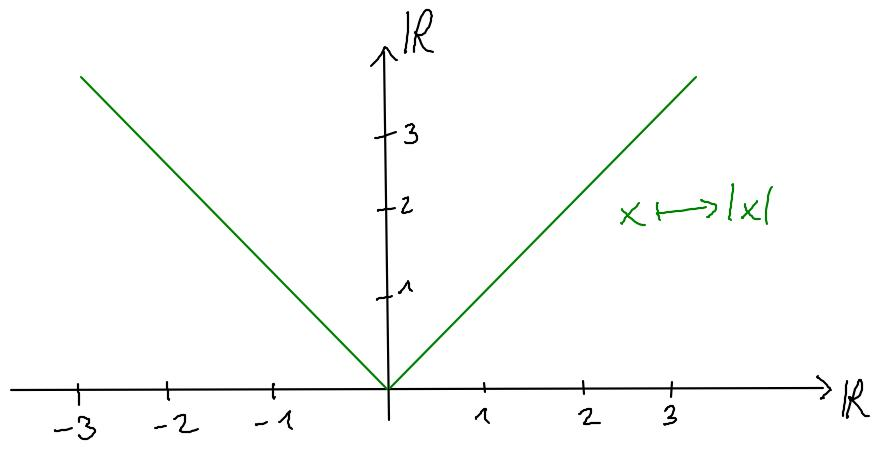
\includegraphics[width=7cm]{./_img/Betrag.jpeg}
        \centering \caption{Graph der Betragsfunktion.}
    \end{minipage}
    \quad
    \begin{minipage}{.48\textwidth}
        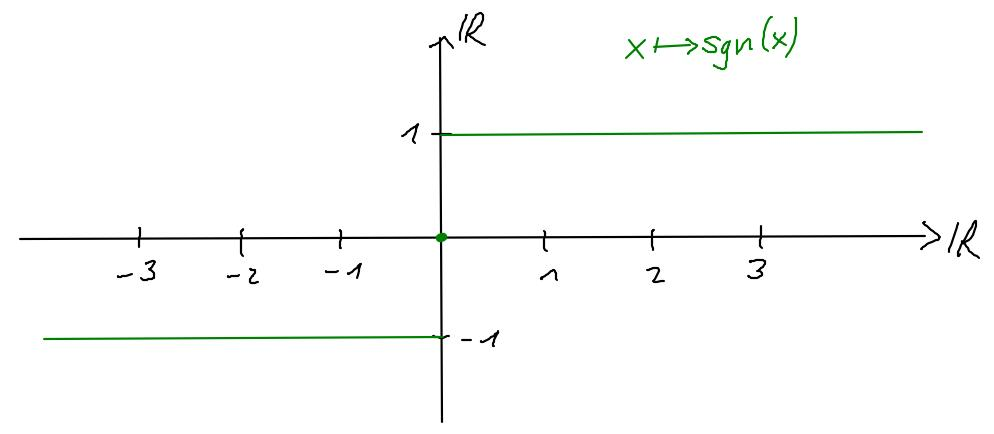
\includegraphics[width=7.5cm]{./_img/Signum.jpeg}
        \centering \caption{Graph der Signumsfunktion}
    \end{minipage}
    \end{figure}
\end{de}


\begin{bsp}
    Beispielsweise ist
    \begin{align*}
        \vert 3\vert &= 3 & \vert -7\vert &=7 & \vert 0\vert=0 \\
        \sgn(3) & = 1 & \sgn(-7) & = -1 & \sgn(0) & = 0
    \end{align*}
\end{bsp}


\begin{bem}[Elementare Regeln für Betrag und Vorzeichen]
    Für eine reelle Zahl $x\in \R$ gelten folgende Aussagen:
    \begin{align*}
        x & = \sgn(x)\cdot \vert x\vert & \vert x \vert & = \sgn(x)\cdot x \\
        \vert x\vert & \ge 0 & x & \le \vert x\vert \\
        \vert -x\vert & = \vert x\vert
    \end{align*}
    Weil das Produkt zweier positiver Zahlen oder zweier negativer Zahlen wieder positiv ist, das Produkt einer positiven mit einer negativen Zahl dagegen negativ ist, gilt:
    \begin{align*}
        \sgn(xy) = \sgn(x)\cdot \sgn(y) && \text{für alle $x,y\in \R$}
    \end{align*}
\end{bem}





\section{Abstand}


\begin{bem}[Abstand im euklidischen Raum]
    Die reellen Zahlen $\R$ werden meist in der „Gestalt“ einer Gerade, der sogenannten \emph{Zahlengerade}, visualisiert. Ebenso können der $\R^2$ als Menge von Punkten in einer Ebene und der $\R^3$ als Menge von Punkten im Raum vorgestellt werden, wobei für ein Tripel $(x,y,z)\in \R^3$ die Zahlen $x,y,z\in \R$ als Koordinaten hinsichtlich eines fixierten Koordinatensystems verstanden werden.
    
    Obwohl es sich bei reellen Zahlen und Vektoren eigentlich um algebraische Objekte handelt, die addiert und vervielfacht werden können, erlaubt es die geometrische Interpretation, sie als „Punkte in einem Raum“ aufzufassen. Zwischen je zwei Punkten auf einer Gerade, in der Ebene oder im Raum kann die Verbindungsstrecke gezogen werden. Die Länge dieser Verbindungsstrecke gibt den \emph{Abstand} der beiden Punkte voneinander an. Der Begriff des Abstands liefert einen von vielen Zugängen zu den Konzepten \emph{Stetigkeit} und \emph{Konvergenz}, der in diesem Kapitel beschritten wird.
    
    Auf der Geraden $\R$, der Ebene $\R^2$ und im Raum $\R^3$ ist der Abstandsbegriff sekundär, indem er als Länge eines Verbindungsvektors definiert wird. Eine direkte Axiomatisierung des Abstandsbegriffs, die auf keinerlei weitere Zusatzstruktur angewiesen ist, geht folgendermaßen:
\end{bem}


\begin{de}[* Abstandsfunktion] \label{def:abstand} \index{Abstandsfunktion} \index{Metrischer Raum} \index{Punkt (in einem metrischen Raum)} \index{Dreiecksungleichung (in metrischen Räumen)}
    Sei $X$ eine beliebige Menge. Eine Funktion $d:X\times X\to \R_{\ge 0}$ heißt eine \textbf{Abstandsfunktion} oder auch \textbf{Metrik}, falls für alle $x,y,z\in X$ gilt:
    \begin{align*}
        d(x,z) \quad&\le\quad d(x,y)+d(y,z) && (\text{Dreiecksungleichung}) \\
        d(x,y) \quad&=\quad d(y,x) && (\text{Symmetrie}) \\
        x=y \quad&\leftrightarrow\quad d(x,y)=0 && (\text{Definitheit})
    \end{align*}
    Ein \textbf{metrischer Raum} ist ein Paar $(X,d)$ bestehend aus einer Menge $X$ und einer Abstandsfunktion $d$ auf $X$. Die Elemente eines metrischen Raums werden auch \textbf{Punkte} genannt. Für Punkte $x,y\in X$ heißt $d(x,y)$ der \textbf{Abstand} von $x$ zu $y$. Ist die konkrete Abstandsfunktion im Kontext klar oder gleichgültig, spricht man schlicht von „dem metrischen Raum $X$“. Der Buchstabe $d$ für die Abstandsfunktion kommt von englisch ``distance''. 
\end{de}


\begin{bem}[zur Dreiecksungleichung]
    Der Name „Dreiecksungleichung“ kommt aus der ebenen Geometrie. Sind $x,y,z\in \R^2$ drei Punkte in der Ebene, die ein Dreieck bilden, so besagt die Dreiecksungleichung, dass „der direkte Weg von $x$ nach $z$ nicht länger als der Umweg über $y$ sein kann“.
    \begin{figure}[ht]
        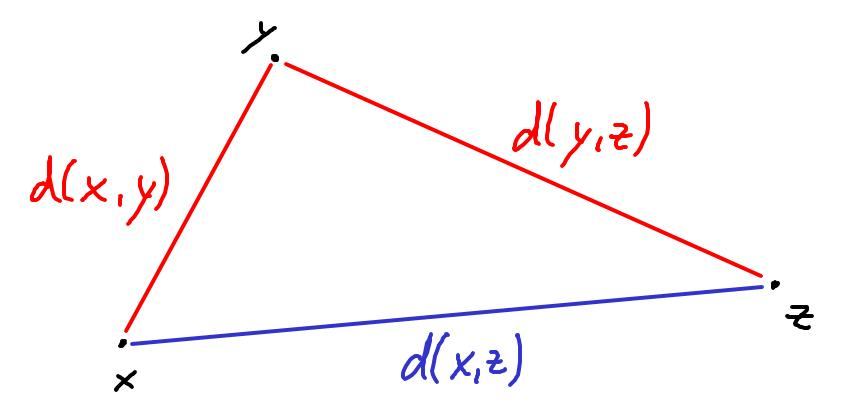
\includegraphics[width=10cm]{./_img/Dreiecksungleichung.jpeg}
        \centering \caption{Dreiecksungleichung: Der direkte Weg $d(x,z)$ ist stets kürzer als der Umweg $d(x,y)+d(y,z)$.}
    \end{figure}
\end{bem}


\begin{bem}
    Manchmal wird die Definitheitseigenschaft auch abgeschwächt, indem anstelle von „$\leftrightarrow$“ nur „$\rightarrow$“ gefordert wird; man spricht dann von einer \emph{Pseudometrik}. Ebenso wird manchmal auch „$\infty$“ als Abstand zugelassen. In jedem Fall aber soll $d$ eine Art „Abstand zwischen Punkten“ bezeichnen.
    
    Die Dreiecksungleichung solltest du dir (mitsamt der bildlichen Erklärung!) einprägen. Bei ihr handelt es sich (auch schon in der Ana1) um das wichtigste Werkzeug zum Abschätzen von Abständen. Versuche, dir die anderen beiden Eigenschaften intuitiv zu merken: Die Symmetrie besagt, dass der Abstand von $x$ zu $y$ gleich dem Abstand von $y$ zu $x$ ist. Die Definitheit impliziert, dass jeder Punkt Abstand Null zu sich selbst hat.
\end{bem}


\begin{de}[Abstand in $\R$]
    Für reelle Zahlen $x,y\in \R$ ist der herkömmliche Abstand definiert durch
        \[ d(x,y) := \vert x -y\vert \]
    Diesbezüglich wird $(\R,d)$ zu einem metrischen Raum, was hier ohne Beweis bleiben soll.\footnote{Einen Beweis findest du z.B. in \cite{AE06}, Satz I.11.4.} Ab sofort wird $\R$ stets mit dieser Abstandsfunktion ausgestattet, ohne dass dies noch einmal ausdrücklich erwähnt würde.
\end{de}


\begin{bsp}
    Beispielsweise ist
        \[ d(5,2)= 3 \qquad\qquad d(-2,5)=7 \qquad\qquad d(3,3)=0 \]
    Für jede reelle Zahl $x\in \R$ ist
        \[ \vert x\vert = \vert x-0\vert = d(x,0) \]
    d.h. der Betrag einer Zahl ist genau ihr Abstand zur Null. 
    \begin{figure}[ht]
        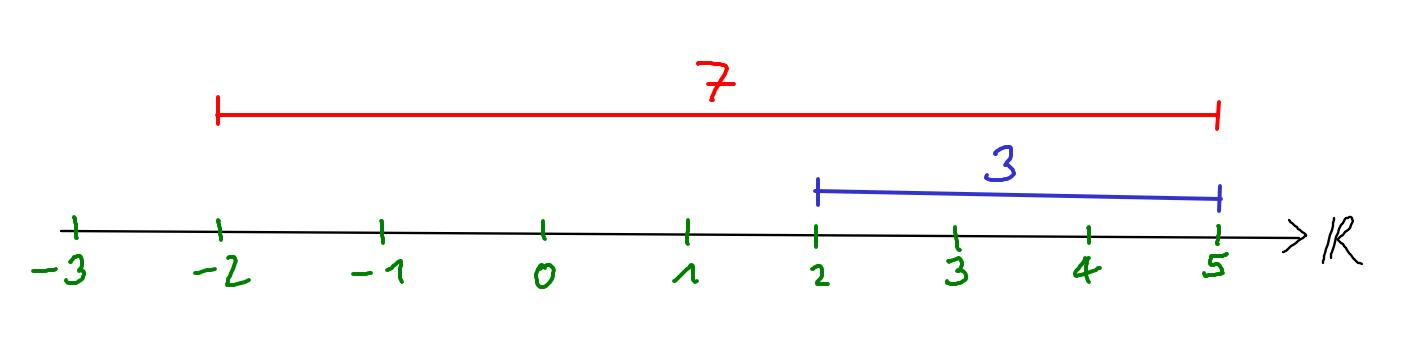
\includegraphics[width=10cm]{./_img/Abstand.jpeg}
        \centering \caption{Abstände auf der reellen Gerade}
    \end{figure}
\end{bsp}


\begin{bsp}[Weitere Metriken] \quad
    \begin{enumerate}
        \item(ebene und räumliche Abstände) In der Ebene $\R^2$, im Raum $\R^3$ und allgemein im Hyperraum $\R^n$ (für ein $n\in \N$) ist der Abstand zweier Punkte gleich der Länge ihrer Verbindungsstrecke. Dies wird in den Analysis-Vorlesungen genauer definiert werden.\footnote{Mehr darüber findest du in \cite{AE06} in Kapitel II.3.} Ich gehe davon aus, dass dir intuitiv klar ist, wie der Abstand zwischen zwei Punkten in der Ebene oder im Raum zu verstehen ist, und werde es ab und zu in einem informellen Sinn nutzen, um mehrdimensionale Beispiele und Illustrationen beisteuern zu können.
        \item(Topologische Datenanalyse) Nicht immer müssen die „Punkte“ eines metrischen Raums eine geometrische Bedeutung besitzen. Beispielsweise wäre ein metrischer Raum $X$ gegeben durch die Menge der Nutzer einer Dating-App, die bei ihrer Anmeldung verschiedene persönliche Vorlieben und Eigenschaften angegeben haben. Für zwei Nutzer $a,b\in X$ könnte dann der „Abstand“ $d(a,b)$ definiert sein als die Anzahl aller Kategorien, in denen $a$ und $b$ verschiedene Präferenzen angegeben haben. Nutzer mit vielen Gemeinsamkeiten wären sich bezüglich dieser Metrik also besonders „nahe“.
    \end{enumerate}
\end{bsp}


\begin{de}[offene Bälle] \label{def:ball} \index{offener Ball}
    Seien $X$ ein metrischer Raum und $a\in X$ ein Punkt. Für $r\in \R_{\ge 0}$ ist der \textbf{offene Ball um $a$ mit Radius $r$} definiert durch
        \[ \bbB_r(a) := \{ x\in X \mid d(a,x)< r\} \]
    $\bbB_r(a)$ ist also die Menge all denjenigen Punkte, deren Abstand zu $a$ strikt kleiner als $r$ ist.
\end{de}


\begin{figure}[ht]
    \begin{minipage}{.48\textwidth}
        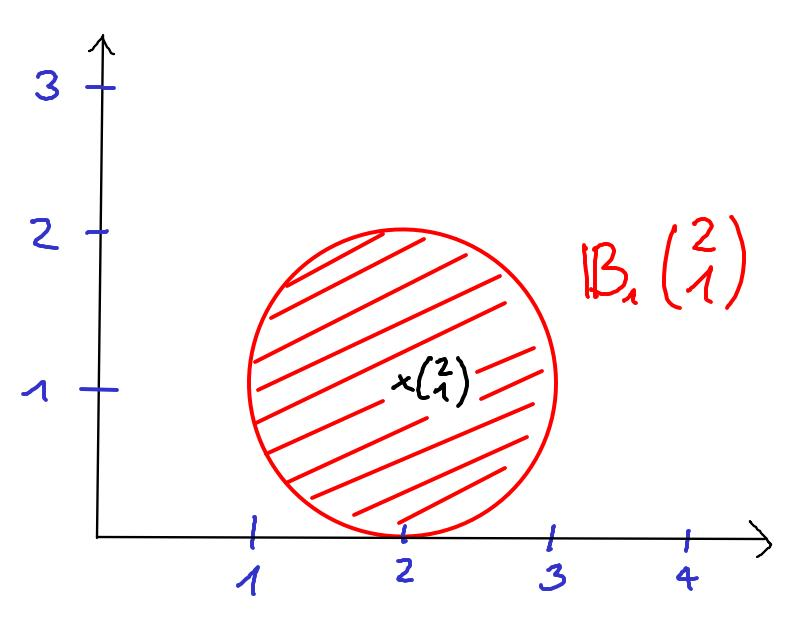
\includegraphics[width=7cm]{./_img/2Dball.jpeg}
        \centering \caption{Der Ball $\bbB_1(2,1)$ im $\R^2$.}
    \end{minipage}
    \quad
    \begin{minipage}{.48\textwidth}
        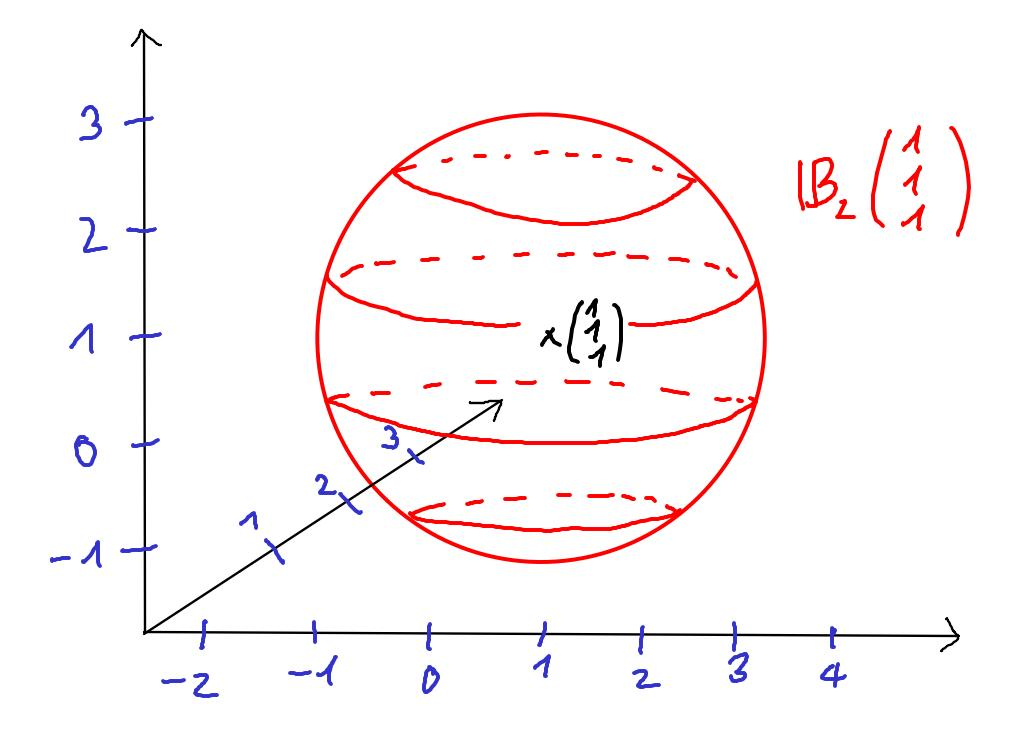
\includegraphics[width=7.5cm]{./_img/3Dball.jpeg}
        \centering \caption{Der Ball $\bbB_2(1,1,1)$ im $\R^3$.}
    \end{minipage}
\end{figure}


\begin{bsp}
    In der Ebene $\R^2$ haben die offenen Bälle die Gestalt einer Kreisscheibe, im Raum $\R^3$ die Gestalt einer Kugel. Beachte, dass die offenen Bälle keinen „Rand“ haben. Denn $\bbB_r(a)$ besteht ja nur aus den Elementen, deren Abstand zu $a$ strikt kleiner als $r$ ist. Diejenigen Elemente, deren Abstand zu $a$ genau gleich $r$ ist (im Zweidimensionalen also genau die Punkte auf dem Kreisrand, im Dreidimensionalen die Punkte auf der Kugeloberfläche), sind nicht in $\bbB_r(a)$ enthalten.
\end{bsp}


\begin{bsp}[offene „Bälle“ in $\R$]
    Betrachte den metrischen Raum $\R$. Für $a=4$ und $r= \frac{3}{2}$ ist
        \[ \bbB_{3/2}(4) = \left\{ x\in \R\mid \vert 4-x\vert <\frac{3}{2} \right\} = \left\{ x\in \R\mid 5/2<x<11/2 \right\} = \left(5/2,11/2\right) \]
    Dies sind genau die Punkte in $\R$, deren Abstand zur $4$ kleiner als $3/2$ ist. Allgemein gilt für reelle Zahlen $a\in \R$ und $r\in \R_{\ge 0}$:
        \[ \bbB_r(a) = (a-r,a+r) \]
    d.h. in $\R$ stimmen die offenen Bälle um $a$ überein mit offenen Intervallen\footnote{zur Definition eines Intervalls siehe \cref{def:intervall}} mit Mittelpunkt $a$.
    
    Dieses Beispiel zeigt, dass die offenen Bälle in allgemeinen metrischen Räumen nicht unbedingt wie „Bälle“ aussehen brauchen.
    \begin{figure}[ht]
        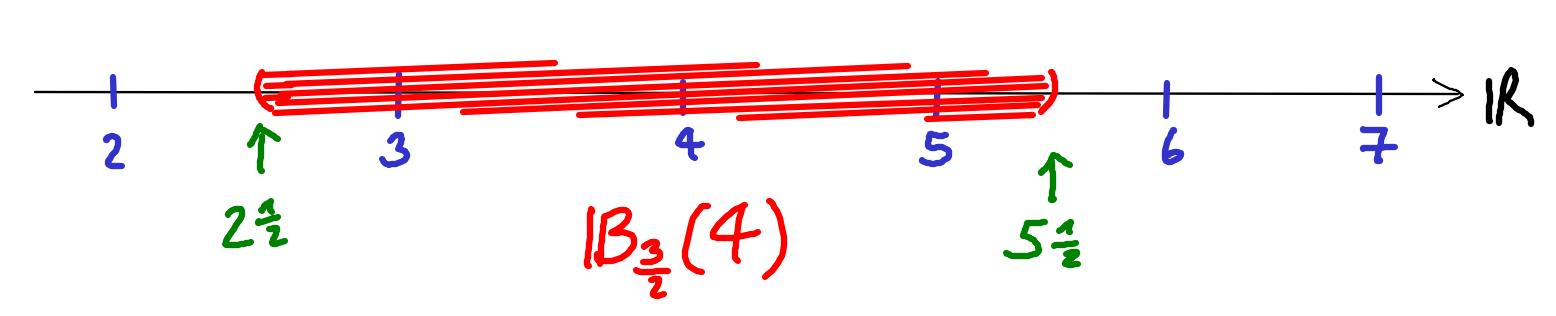
\includegraphics[width=9.5cm]{./_img/1Dball.jpeg}
        \centering \caption{Der offene Ball $\bbB_{3/2}(4)$ in $\R$.}
    \end{figure}
\end{bsp}


\begin{de}[Umgebung in einem metrischen Raum] \label{def:umgebung} \index{Umgebung (Metrische Räume)} \index{innerer Punkt}
    Seien $X$ ein metrischer Raum, $U\subseteq X$ eine Teilmenge und $a\in U$ ein Punkt. $a$ heißt ein \textbf{innerer Punkt von $U$} und $U$ heißt eine \textbf{Umgebung von $a$}, wenn es ein (möglicherweise winzig kleines) $\varepsilon\in \R_{>0}$ gibt mit $\bbB_\varepsilon(a)\subseteq U$.
    \begin{figure}[ht!]
        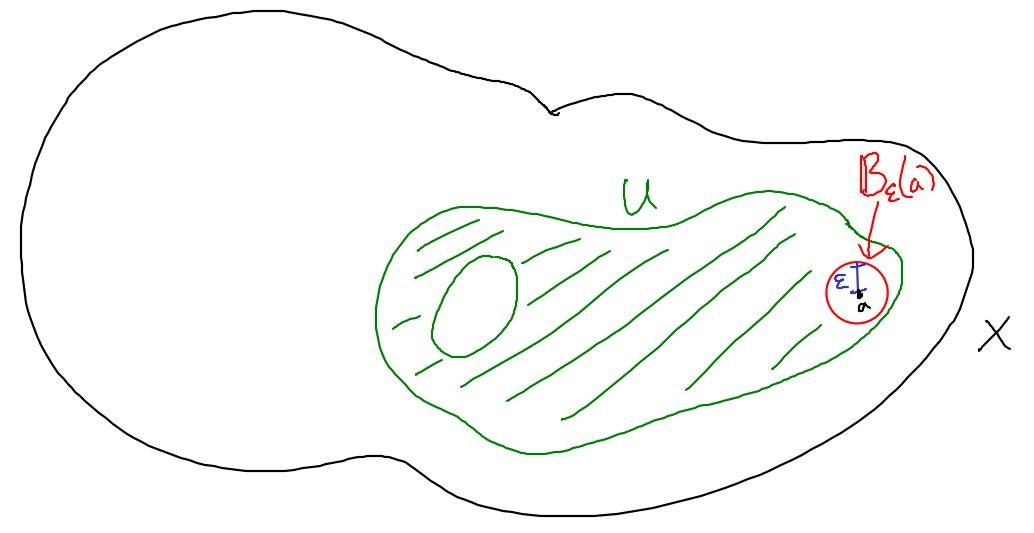
\includegraphics[width=10.5cm]{./_img/Umgebung.jpeg}
        \centering \caption{Im metrischen Raum $X$ ist $U$ eine Umgebung des Punkts $a$, weil sie den $\varepsilon$-Ball $\bbB_\varepsilon(a)$ umfasst.}
    \end{figure}
\end{de}


\begin{bsp}
    Es gilt:
    \begin{enumerate}
        \item Das abgeschlossene Intervall $[0,4]$ ist eine Umgebung der $2$, da $\bbB_1(2)\subseteq [0,4]$.
        \item Dagegen ist $[0,4]$ keine Umgebung der $0$, denn für jedes $\varepsilon\in\R_{>0}$ ist $-\varepsilon/2 \in \bbB_\varepsilon(0)\setminus [0,4]$.
        \item Betrachten wir das Quadrat $Q:=[0,1]\times [0,1]\subseteq \R^2$, so ist $Q$ weder eine Umgebung der Eckpunkte, noch aller weiteren Randpunkte. Denn jeder noch so kleine $\varepsilon$-Ball um einen dieser Randpunkte lugt ja immer ein Stück über den Quadratrand hinaus, ist also nicht vollständig im Quadrat enthalten. Allerdings ist $Q$ eine Umgebung jedes der Punkte im „Inneren“ des Quadrats. Diese letzte Behauptung ist nicht wirklich beweisbar, weil es sich dabei gerade um eine \emph{Definition} des „Inneren“ handelt.
        \item Für einen metrischen Raum $X$ und einen Punkt $a\in X$ ist jeder $\varepsilon$-Ball um $a$ trivialerweise eine Umgebung von $a$, da $\bbB_\varepsilon(a)\subseteq\bbB_\varepsilon(a)$.
    \end{enumerate}
    \begin{figure}[ht!]
        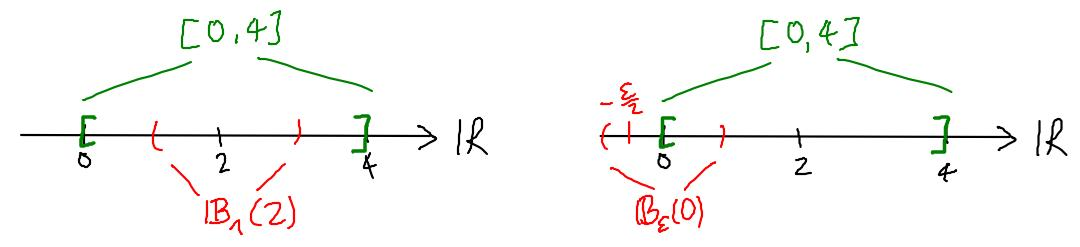
\includegraphics[width=\textwidth]{./_img/Intervallpunkte.jpeg}
        \centering \caption{Das Intervall $[0,4]$ ist eine Umgebung der $2$, aber nicht der $0$.}
        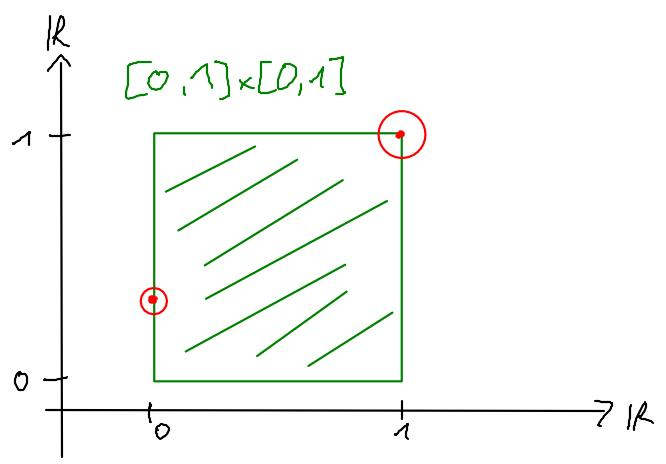
\includegraphics[width=10cm]{./_img/Quadratpunkte.jpeg}
        \centering \caption{Die Randpunkte des Quadrats sind keine inneren Punkte, weil jeder $\varepsilon$-Ball ein Stück weit „über den Rand hinaus reicht“.}
    \end{figure}
\end{bsp}


\begin{bem}[Intuition]
    Die Ansicht, einen „Raum“, wie etwa den euklidischen dreidimensionalen Raum, als eine „Punktmenge“ aufzufassen, ist vergleichsweise jung und trug wesentlich zur Entstehung des Mengenbegriffs, der bei Cantor aus der Untersuchung von Nullstellen gewisser Funktionen $\R \to \R$ erwuchs, bei. Vormals waren der Raum oder die reelle Gerade eher als eine Art „Kontinuum“ verstanden, auf dem zwar einzelne Punkte ausgezeichnet werden können, das aber eine über die Ansammlung von Punkten hinausgehende Qualität der „Kontinuierlichkeit“ besitzt. Auch über die physikalische Realität des Punktbegriffs, eines ausdehnungslosen Orts im Raum oder in der Zeit, lässt sich streiten.\footnote{Mit einer Formalisierung der Konzepte „Nähe“ und „Abweichung“, die unabhängig vom Vorhandensein von Punkten ist, beschäftigt sich die \href{https://en.wikipedia.org/wiki/Pointless_topology}{punktfreie Topologie}, die bislang aber noch keinen Einzug in den mathematischen Mainstream gefunden hat.}
    
    In Physik und Stochastik können meist nur Näherungsbereiche für einen Punkt angegeben werden. Beispielsweise ist die Wahrscheinlichkeit dafür, dass ein Dartspieler exakt die Mitte des Dartboards trifft, exakt $0{,}0\%$, da es sich bei der „Mitte des Boards“ um eine mathematische Idealisierung handelt. Dagegen kann für das Treffen des etwa 1cm breiten Bullseye durchaus eine positive Wahrscheinlichkeit angegeben werden, die bei einem professionellen Spieler wie zum Beispiel Phil ``The Power'' Taylor weit im zweistelligen \%-Bereich liegt.
    
    Beim Bullseye-Feld handelt es sich um eine „Umgebung“ des Board-Mittelpunkts. Per Definition beinhaltet eine Umgebung $U$ eines Punkts $a$ einen $\varepsilon$-Ball. Der Punkt hat also einen gewissen „Puffer“ um sich herum in $U$. Sofern wir den Punkt $a$ nur bis auf eine Genauigkeit in der Größe von $\varepsilon$ verorten können, kann dennoch garantiert werden, dass $U$ den Punkt $a$ enthält.
\end{bem}





\section{Zahlenfolgen}


\begin{bem}[Das Zeichen „$\N$“] \label{natzahlen}
    In diesem Abschnitt (und auch überall sonst in diesem ganzen Skript) wird die Menge der natürlichen Zahlen, sofern die Null eingeschlossen ist, mit „$\N_0$“ bezeichnet und, sofern die Null ausgeschlossen ist, mit „$\N_{\ge 1}$“. In Situationen, in denen es keine Rolle spielt, ob die Null dabei ist oder nicht, schreibe ich einfach nur „$\N$“.
\end{bem}


\begin{de}[Folge] \label{def:folge} \index{Folge}
    Eine \textbf{Folge} ist eine Familie von Objekten $(a_n)_{n\in \N}$, deren Indexmenge die Menge $\N$ der natürlichen Zahlen ist. Ist $n\in \Z$ eine beliebige ganze Zahl, so spricht man manchmmal auch bei Familien, deren Indexmenge $\Z_{\ge n}$ ist, von Folgen. In diesem Fall starten die Indizes nicht bei Eins oder Null, sondern bei $n$. Der Begriff der Folge ist also nicht präzise umrissen, spricht man aber von „der beliebigen Folge $(a_n)$“ so ist damit gemeint, dass die Indexmenge gleich $\N$ (mit oder ohne Null) ist.
    
    Sind $A$ eine Menge und $(a_n)_{n\in \N}$ eine Folge, deren Einträge allesamt in $A$ liegen, so spricht man von einer \emph{Folge von Elementen aus $A$} oder einer „$A$-wertigen Folge“. Nach \cref{def:mengenpotenz} bezeichnet
    \[ A^\N := \{ (a_n)_{n\in \N} \mid \forall n\in \N: a_n\in A \} \]
    die Menge aller Folgen mit Einträgen aus $A$. Im Spezialfall $A=\R$ spricht man von \textbf{reellen Zahlenfolgen} oder auch \textbf{reellwertigen Folgen}. Analog spricht man von rationalen Zahlenfolgen, Folgen ganzer Zahlen oder komplexen Zahlenfolgen, falls es sich um Elemente von $\Q^\N$, $\Z^\N$ oder $\C^\N$ handelt.
\end{de}


\begin{nota}
    Folgen lassen sich sowohl durch eine exakte Angabe definieren, etwa
    \begin{align*}
        (n^2)_{n\in \N_0}
    \end{align*}
    als auch durch eine suggestive Aufzählung der ersten paar Folgenglieder, etwa
        \[ 0,\quad 1,\quad 4,\quad 9,\quad 16,\quad 25,\quad\dots \]
    Die „Definition durch Auflistung“ ist allerdings nicht mathematisch präzise und sollte nur dann benutzt werden, wenn wirklich unmissverständlich klar ist, welche Folge gemeint ist. Würdest du etwa erahnen, dass mit
        \[ 0,\quad 2,\quad 12,\quad 36,\quad 80,\quad 150,\quad 252,\quad 392,\quad \dots\]
    die Zahlenfolge $(n^2\cdot (n+1))_{n\in \N_0}$ gemeint sein soll?
\end{nota}


\begin{bem}[Folge vs. Menge ihrer Einträge]
    Eine Folge $(a_n)_{n\in \N}$ ist nicht mit der Menge ihrer Einträge $\{a_n\mid n\in \N\}$ zu verwechseln.\footnote{vgl. \cref{mengeeinerfamilie}} Beispielsweise sind die beiden Zahlenfolgen
    \begin{align*}
        1,\quad 2,\quad 3,\quad 1,\quad 2,\quad 3,\quad 1,\quad 2,\quad \dots \\
        1,\quad 3,\quad 2,\quad 1,\quad 3,\quad 2,\quad 1,\quad 3,\quad \dots
    \end{align*}
    voneinander verschieden, während die Mengen ihrer Einträge (nämlich nur $1$, $2$ und $3$) übereinstimmen.
\end{bem}


\begin{bsp}
    Beispiele für reelle Zahlenfolgen sind:
    \begin{enumerate}
        \item Die Folge der Primzahlen $2,3,5,7,11,\dots$.
        \item Die Folge der natürlichen Zahlen $0,1,2,3,4,\dots$.
        \item Die „alternierende Folge“ $((-1)^n)_{n\in \N_0}$. Also $1,-1,1,-1,1,-1,1,\dots$.
        \item Die Folge $0,1,-1,2,-2,3,-3,4,\dots$. Es handelt sich um diejenige Folge $(a_n)_{n\in \N_0}$ mit den Einträgen
        \begin{align*}
            a_n := \begin{cases}
                -\frac{n}{2} & n\ \text{ist eine gerade Zahl} \\
                \frac{n+1}{2} & n\ \text{ist eine ungerade Zahl}
            \end{cases} && n \in \N_0
        \end{align*}
        \item Die Folge der Kehrwerte natürlicher Zahlen $(1/n)_{n\in \N_{\ge 1}}$. Das ist  $1,\frac{1}{2},\frac{1}{3},\frac{1}{4},\frac{1}{5},\dots$. Bei dieser Folge gehen die Indizes erst bei Eins los.
        \item Die Folge $\left(\frac{n}{n+1}\right)_{n\in \N_0}$. Also $0,\frac{1}{2},\frac{2}{3},\frac{3}{4},\frac{4}{5},\dots$.
        \item Die „konstante Folge“ $(3)_{n\in \N}$. Also $3,3,3,3,3,\dots$.
        \item Für $q\in \R$ die Folge der $q$-Potenzen $(q^n)_{n\in \N_0}$ Im Fall $q=2$ erhielte man beispielsweise die Folge der Zweierpotenzen $1,2,4,8,16,\dots$.
    \end{enumerate}
    In all diesen Beispielen gehorchen die Folgenglieder einer einfachen Regel. Dies muss aber nicht immer der Fall sein. Eine Folge darf auch völlig chaotisch sein und ihre Einträge brauchen keinem Muster zu gehorchen. Möglichst chaotische Folgen können mit einem Programm zur Berechnung von Zufallszahlen erzeugt werden.
        
    Hier ist noch ein Beispiel für eine Folge, deren Einträge mal keine Zahlen sind:
    \begin{enumerate}[(9)]
        \item Die Folge $(\{1,\dots , n\})_{n\in \N_0}$, deren Einträge die „Anfangsstücke“ von $\N_{\ge 1}$ sind. Also
            \[ \emptyset\ ,\quad \{1\}\ ,\quad \{1,2\}\ ,\quad \{1,2,3\}\ ,\quad \{1,2,3,4\}\ , \quad \dots \]
        Dies ist keine Zahlenfolge, sondern eine Folge von Mengen. Sie besitzt die Eigenschaft, dass für jedes $n\in \N_0$ ihr $n$-ter Eintrag eine Menge ist, die genau $n$-viele Elemente enthält.
    \end{enumerate}
    Eine riesige Datenbank ganzzahliger Zahlenfolgen ist die \href{https://oeis.org/}{On-Line Encyclopedia of Integer Sequences}.
\end{bsp}


\begin{de}[Beschränktheit] \index{beschränkte Folge}
    Eine reelle Zahlenfolge $(a_n)_{n\in \N}\in \R^\N$ heißt \textbf{nach oben beschränkt} bzw. \textbf{nach unten beschränkt}, falls die Menge ihrer Einträge $\{a_n\mid n\in \N\}$ eine nach oben bzw. nach unten beschränkte Teilmenge von $\R$ im Sinne von \cref{def:schranken} ist. Konkret ist die Folge $(a_n)_{n\in \N}$ also genau dann
    \begin{itemize}
        \item \textbf{nach oben beschränkt}, falls es eine Zahl $M\in \R$ gibt derart, dass $a_n\le M$ für alle $n\in \N$ ist. In diesem Fall heißt ein solches $M$ eine \textbf{obere Schranke} für $(a_n)_{n\in \N}$.
        \item \textbf{nach unten beschränkt}, falls es eine Zahl $M\in \R$ gibt mit $a_n\ge M$ für alle $n\in \N$. In diesem Fall heißt ein solches $M$ eine \textbf{untere Schranke} für $(a_n)_{n\in \N}$.
        \item \textbf{beschränkt}, falls sie sowohl nach oben als auch nach unten beschränkt ist.
        \item \textbf{unbeschränkt}, wenn sie nicht beschränkt ist.
    \end{itemize}
\end{de}


\begin{bsp} Es gilt:
    \begin{enumerate}
        \item Die Folge $\left(\frac{n}{n+1}\right)_{n\in \N}$ ist nach unten durch $0$ und nach oben durch $1$ beschränkt.
        \item Die Folge $2,3,5,7,11,\dots$ der Primzahlen ist nach oben unbeschränkt. Dies ist die Aussage des berühmten \emph{Satzes von Euklid} aus \cref{euklid}.
        \item Die alternierende Folge $((-1)^n)_{n\in \N}$ ist beschränkt, da sie nach oben durch $1$ und nach unten durch $-1$ beschränkt ist.
    \end{enumerate}
    Da die Beschränktheit einer Folge allein von der Menge ihrer Einträge abhängt, ist sie unempfindlich gegenüber einer Änderung der Reihenfolge der Folgeneinträge.
\end{bsp}


\begin{de}[Monotonie] \index{Monotonie (von Folgen)} \index{wachsende Folge} \index{fallende Folge}
    Eine Folge reeller Zahlen $(a_n)_{n\in \N}\in \R^\N$ heißt
    \begin{itemize}
        \item \textbf{(monoton) wachsend}, falls für jedes $n\in \N$ gilt, dass $a_{n+1}\ge a_n$.
        \item \textbf{(monoton) fallend}, falls für jedes $n\in \N$ gilt, dass $a_{n+1}\le a_n$.
        \item \textbf{monoton}, falls sie wachsend oder fallend ist.
    \end{itemize}
    Gilt sogar $a_{n+1}>a_n$ für alle $n\in \N$, so sagt man auch, die Folge sei \emph{strikt wachsend}. Ähnlich definiert man \emph{strikt fallend}.
\end{de}


\begin{bsp}
Es gilt:
    \begin{enumerate}
        \item Die alternierende Folge $((-1)^n)_{n\in \N}$ ist nicht monoton, da zum Beispiel $(-1)^3< (-1)^4$ aber auch $(-1)^4>(-1)^5$.
        \item Die Folge $\left(\frac{n}{n+1}\right)_{n\in \N}$ ist strikt wachsend.
        \begin{bew}
            Für jedes $n\in \N$ ist
            \begin{align*}
                \frac{(n+1)}{(n+1)+1} - \frac{n}{n+1} & = \frac{1}{(n+2)(n+1)} >0
            \end{align*}
            sodass $\frac{(n+1)}{(n+1)+1} > \frac{n}{n+1}$ ist. \qed
        \end{bew}
        \item Für $q\in \R_{\ge 1}$ ist die Folge $(q^n)_{n\in \N}$ monoton wachsend.
        \begin{bew}
            Weil für jedes $n\in \N$ gilt:
            \begin{align*}
                q^{n+1} & = q \cdot q^n \\
                & \ge 1 \cdot q^n && (\text{wegen $q\ge 1$ und $q^n>0$})\\
                & = q^n &&&& \qed
            \end{align*}
        \end{bew}
    \end{enumerate}
\end{bsp}


\begin{de}[``eventually''] \label{def:eventually} \index{eventually (Folgenverhalten)}
    Seien $(a_n)_{n\in \N}$ eine Folge und $E$ eine Eigenschaft. Ich sage, die Folge $(a_n)_{n\in \N}$
    \begin{itemize}
        \item[] \textbf{besitzt die Eigenschaft $E$ für hinreichend große $n$}\footnote{Im Englischen ist die Sprechweise ``the sequence \href{https://en.wikipedia.org/wiki/Eventually_(mathematics)}{eventually} satisfies $E$'' üblich. Leider besitzt sie kein etabliertes Pendant im Deutschen.},
    \end{itemize}
    falls es ein $N\in \N$ gibt derart, dass die Folge $a_N,a_{N+1},a_{N+2},\dots$ die Eigenschaft $E$ besitzt. Salopp gesagt: „Es gibt einen Zeitpunkt $N$ derart, dass diejenige Folge, bei der erst zum Zeitpunkt $N$ eingestiegen wird, die Eigenschaft $E$ besitzt.“
\end{de}


\begin{bsp} \label{bsp:eventually} \quad
    \begin{enumerate}
        \item Die Folge
            \[ 0,\quad -1,\quad -2,\quad -1,\quad 0,\quad 1,\quad 2,\quad 3,\quad 4, \quad 5,\dots \]
        ist nicht monoton. Sie könnte aber zu einer strikt wachsenden Folge gemacht werden, ließe man die ersten zwei Folgenglieder weg. Somit ist sie „wachsend für hinreichend große $n$“.
        \item Die alternierende Folge $((-1)^n)_{n\in \N}$ ist dagegen nicht einmal für hinreichend große $n$ wachsend, denn egal wie spät wir auch einsteigen, immer wieder geht es von $-1$ zu $1$ herauf und von $1$ zu $-1$ herunter.
        \item Ist $\varepsilon \in \R_{>0}$ eine (unter Umständen winzig kleine) positive reelle Zahl, so sind die Einträge der Folge $\left(\frac{1}{n}\right)_{n\in \N}$ dennoch für hinreichend große $n$ (um genau zu sein für $n> \frac{1}{\varepsilon}$) kleiner als $\varepsilon$. Mit anderen Worten: Die Brüche $\frac{1}{n}$ werden „für hinreichend große $n$ beliebig klein“.
    \end{enumerate}
\end{bsp}





\section{Folgenkonvergenz}


\begin{bem}[Intuition]
    \begin{figure}[ht]
        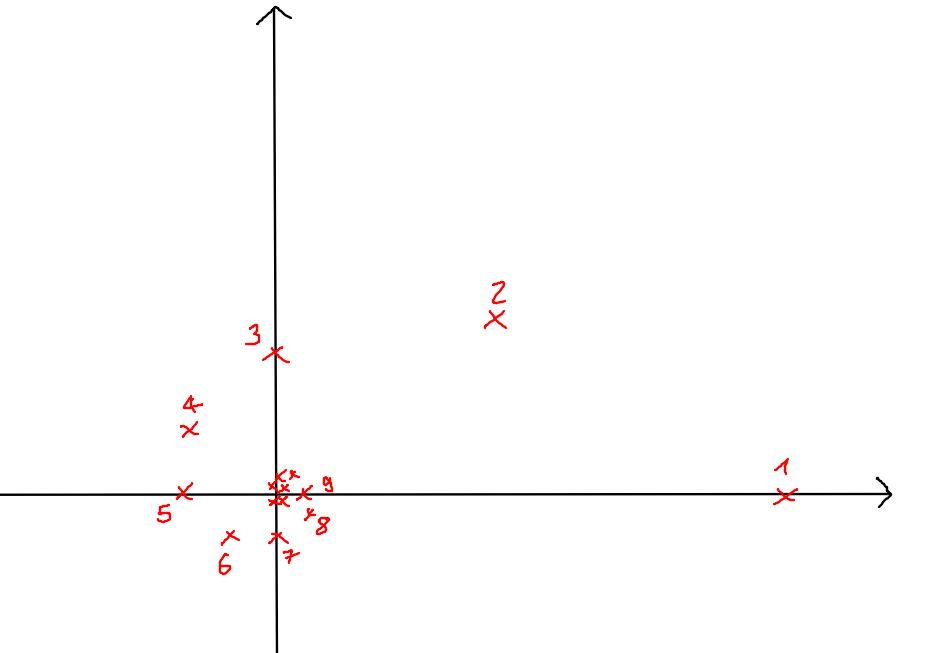
\includegraphics[width=10cm]{./_img/Spirale.jpeg}
        \centering \caption{Eine konvergente Folge von Punkten in der Ebene}
    \end{figure}
    Betrachten wir einmal eine Folge von Punkten in der Ebene, die sich spiralenförmig dem Ursprung annähert. Konkret könnte man
    \begin{align*}
        a_n & := \frac{1}{n}\cdot \begin{pmatrix}
            \cos(n\cdot \pi/4) \\
            \sin(n\cdot \pi/4)
        \end{pmatrix} && n\in \N
    \end{align*}
    definieren, aber das soll gerade keine Rolle spielen.
    
    Du siehst, dass die Folgenglieder dem Koordinatenursprung immer näher kommen, dass sie ihm „für hinreichend große $n$ beliebig nahe kommen“. Genau das heißt Konvergenz.
\end{bem}


\begin{de}[Folgenkonvergenz] \label{def:konvergenz} \index{konvergente Folge} \index{Grenzwert} \index{divergente Folge} \index{Limes}
    Seien $X$ ein metrischer Raum, $(a_n)_{n\in \N}$ eine Folge in $X$ und $a\in X$ ein Punkt. Man sagt, die Folge $(a_n)_{n\in \N}$ \textbf{konvergiert} gegen $a$, falls eine der folgenden beiden äquivalenten Aussagen gilt:
    \begin{enumerate}[(i)]
        \item Für jede (noch so kleine) Umgebung $U$ von $a$ gilt: Für hinreichend große $n$ liegen alle $a_n$'s in $U$.
        \item Für jedes (noch so kleine) $\varepsilon \in \R_{>0}$ gibt es ein $N\in \N$ derart, dass $d(a_n,a)<\varepsilon$ für alle $n\in \N_{\ge N}$. Als Formel:
        \begin{align*}
            \forall\varepsilon\in \R_{>0}\ \exists N\in\N\ \forall n\in \N_{\ge N}:\ d(a_n,a)<\varepsilon
        \end{align*}
    \end{enumerate}
    In diesem Fall heißt $a$ ein \textbf{Grenzwert} oder \textbf{Limes} der Folge $(a_n)_{n\in \N}$. Man schreibt
        \[ \lim_{n\to\infty}a_n=a \qquad\text{oder}\qquad a_n\xrightarrow[n\to \infty]{} a \]
    Eine Folge, die einen Grenzwert besitzt, heißt \textbf{konvergent}. Andernfalls heißt sie \textbf{divergent}.
\end{de}


\begin{bew}[*]
    (i)$\to$(ii): Sei $\varepsilon\in \R_{> 0}$ beliebig. Weil der $\varepsilon$-Ball $\bbB_\varepsilon(a)$ eine Umgebung von $a$ ist, folgt aus (i), dass die $a_n$'s für hinreichend großes $n$ in $\bbB_\varepsilon(a)$ liegen, also dass es ein $N\in \N$ gibt derart, dass $a_n\in \bbB_\varepsilon(a)$ für alle $n\in \N_{\ge N}$. Per Definition des Balles $\bbB_\varepsilon(a)$ ist dies genau die Aussage von (ii). \\[0.5em]
    (ii)$\to$(i): Sei $U\subseteq X$ eine beliebige Umgebung von $a$. Nach \cref{def:umgebung} gibt es dann ein $\varepsilon\in \R_{>0}$ mit $\bbB_\varepsilon(a)\subseteq U$. Nach (ii) gibt es ein $N\in \N$ derart, dass $d(a_n,a)<\varepsilon$ für alle $n\in \N_{\ge N}$, d.h. für hinreichend großes $n$ haben die $a_n$'s einen Abstand von weniger als $\varepsilon$ von $a$. Nach \cref{def:ball} heißt das gerade, dass die $a_n$'s in $\bbB_\varepsilon(a)$ liegen für hinreichend große $n$, wegen $\bbB_\varepsilon(a)\subseteq U$ also auch in $U$. \qed
\end{bew}


\begin{bem}[„Sei $\varepsilon>0$“] \index{Epsilontik}
    Diese Grenzwertdefinition ist vergleichsweise jung: sie stammt aus dem 19. Jahrhundert und wurde durch Cauchy\footnote{\href{https://de.wikipedia.org/wiki/Augustin-Louis_Cauchy}{Augustin-Louis Cauchy (1789 - 1857)}} und Weierstraß\footnote{\href{https://de.wikipedia.org/wiki/Karl_Weierstra\%C3\%9F}{Karl Weierstraß (1815 - 1897)}} populär. Bis dahin herrschte in der Mathematik ein eher „intuitiver“ Umgang mit Grenzwerten vor.
    
    Definition (i) ist prägnant, recht leicht zu merken und geeignet, um manche allgemeine Sätze zu beweisen. Dagegen ist das Logik-Monstrum (ii) diejenige Definition, die relevant wird, wenn du von einer konkreten Zahlenfolge ausrechnen willst, dass sie konvergiert.
    
    In der Analysis hat es sich eingebürgert, in Definitionen und Beweisen jene Abstände, die „beliebig klein“ werden können, mit einem Epsilon $\varepsilon$ zu notieren. Aus diesem Grund spricht man bei Definitionen und Beweisen der Analysis, die exzessiven Gebrauch von $\varepsilon$'s machen, von „Epsilontik“.
\end{bem}


\begin{bsp} \label{bsp:konvergenz}
    Die durch
    \begin{align*}
        a_n &:= \frac{n}{n+1} && n\in \N
    \end{align*}
    definierte reelle Folge $(a_n)_{n\in \N}\in \R^\N$ konvergiert gegen $1$.
\end{bsp}


\begin{figure}[ht]
    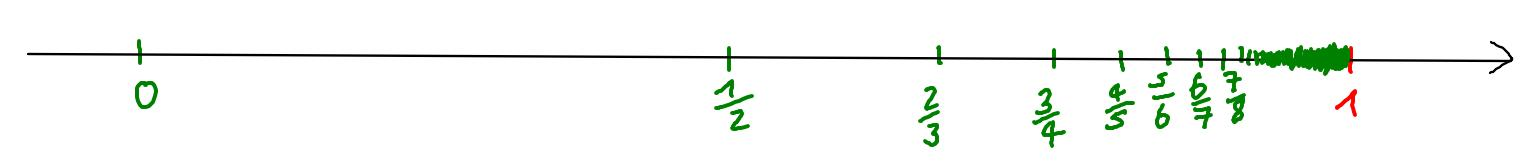
\includegraphics[width=14cm]{./_img/Konvergenzbsp.jpeg}
    \centering \caption{Die Folge $\left(\frac{n}{n+1}\right)_{n\in \N}$ konvergiert gegen $1$.}
\end{figure}


\begin{bem}
    Bevor wir versuchen, für diese Aussage einen Bilderbuchbeweis hinzuschreiben, wollen wir „auf dem Skizzenblatt“ erstmal ein paar Überlegungen anstellen:
    
    Nach \cref{def:konvergenz}(ii) müssen wir für ein beliebiges $\varepsilon \in \R_{>0}$ ein $N\in \N$ finden mit der Eigenschaft, dass für alle $n\in \N_{\ge N}$ gilt:
    \begin{align*}
        \varepsilon &  > d\left(1,\frac{n}{n+1}\right)
    \end{align*}
    Mit ein paar Umformungen ergibt sich:
    \begin{align*}
        d\left(1,\frac{n}{n+1}\right) & = \left| 1-\frac{n}{n+1}\right| \\
        & = \left| \frac{n+1}{n+1} - \frac{n}{n+1} \right| \\
        & = \left| \frac{1}{n+1}\right| \\
        & = \frac{1}{n+1} & (\text{da $n\in \N$})
    \end{align*}
    Die Ungleichung $\varepsilon >d(1,n/(n+1))$ lautet also
        \[ \varepsilon > \frac{1}{n+1} \]
    Mit den Umformungen aus \cref{bsp:ungleichungumstellen} kann dies nach $n$ umgestellt werden:
        \[ n > \frac{1}{\varepsilon} -1  \]
    Wählen wir also für $N$ die nächstgrößere natürliche Zahl oberhalb von $1/\varepsilon$, indem wir $1/\varepsilon$ aufrunden (man könnte für $N$ auch jede weitere Zahl, die größer als $1/\varepsilon -1$ ist, verwenden). Dann sind sowohl $N$ als auch alle $n\in \N_{>N}$ größer als $1/\varepsilon- 1$, sodass die Ungleichung aufgeht.
    
    Damit haben wir die Aufgabe auf dem Schmierblatt gelöst. Im finalen Beweis lassen wir die Überlegungen, die uns zur Wahl von $N$ geführt haben, weg. Dies tritt häufig in Analysis-Beweisen auf: die Beweise unterdrücken den Gedankenprozess, der zu ihrem Auffinden geführt hat und verlaufen genau in die entgegengesetzte Richtung:
\end{bem}


\begin{bew}
    Es sei $\varepsilon \in \R_{>0}$ beliebig. Sei $N\in \N$ irgendeine natürliche Zahl, die größer als $1/\varepsilon$ ist. Für alle $n\in \N_{\ge N}$ gilt dann:
    \begingroup
    \allowdisplaybreaks
    \begin{align*}
        d(1,a_n) & = \left| 1-\frac{n}{n+1}\right| \\
        & = \left| \frac{1}{n+1} \right| \\
        & = \frac{1}{n+1} \\
        & \le \frac{1}{N} & (\text{da $N\le n$})\\
        & < \varepsilon & (\text{da $N> 1/\varepsilon$})
    \end{align*}
    \endgroup
    Somit liegen ab dem $N$-ten Eintrag alle Folgenglieder in $\bbB_\varepsilon(1)$. Da $\varepsilon \in \R_{>0}$ beliebig gewählt war, ist damit bewiesen, dass die $a_n$'s gegen $1$ konvergieren. \qed
\end{bew}


\begin{bem}
    Beachte, dass die Tatsache, ob eine Folge konvergiert oder divergiert, eine reine Eigenschaft des „Langzeitverhaltens“ dieser Folge ist. Die ersten paar Millionen Folgenglieder haben für sich allein keinen Einfluss auf das Konvergenzverhalten, weil die Folge ja ab dem dreimillionsten Eintrag plötzlich eine ganz andere Richtung einschlagen könnte. (Die Folgen, mit denen du es in der Vorlesung zu tun hast, unterliegen aber meist einem einfachen Muster, das spätestens nach ein paar Dutzend Folgengliedern ersichtlich sein sollte.)
\end{bem}


\begin{bsp}[Konstante Folgen konvergieren]
    Seien $X$ ein metrischer Raum und $x \in X$ ein beliebiger Punkt. Dann konvergiert die konstante Folge $(x)_{n\in \N}$ gegen $x$.
        \[ x,x,x,x,\dots \qquad \xrightarrow[n\to \infty]{} x \]
\end{bsp}
    
    
\begin{bew}
    Sei $U$ eine beliebige Umgebung von $x$. Wegen $x\in U$ liegt die konstante Folge $(x)_{n\in \N}$ vollständig in $U$. Weil die Umgebung $U$ beliebig gewählt war, konvergiert die Folge nach \cref{def:konvergenz}(i) also gegen $x$.
\end{bew}


\begin{bem}
    Der Satz lässt sich dahingehend verallgemeinern, dass auch schon jede Folge, die für hinreichend große $n$ konstant gleich $x$ ist, gegen $x$ konvergiert. In diesem Fall liegt die Folge zwar nicht mehr unbedingt vollständig in der Umgebung $U$, aber immer noch für hinreichend große $n$, und dies reicht ja schon aus für das Vorliegen von Konvergenz.
\end{bem}


\begin{vorschau}[* Ordnungstopologie]
    Es ist möglich, Konvergenz reellwertiger Folgen rein ordnungstheoretisch zu definieren. Sind $a\in \R$ und $(a_n)_{n\in \N}$ eine Folge reeller Zahlen, so kann man definieren, dass die $a_n$'s gegen $a$ konvergieren genau dann, wenn für alle $x\in \R_{<a}$ und alle $y\in \R_{>a}$ gilt, dass die $a_n$'s für hinreichend große $n$ allesamt größer als $x$ und kleiner als $y$ sind. Auf dieser Weise lässt sich auch die Konvergenz von Folgen auf der erweiterten Zahlengerade $\bar \R$ definieren. Zum Beispiel gälte dann $\lim_{n\to\infty} n^2=\infty$.
    
    Das dahinterliegende Prinzip heißt \href{https://de.wikipedia.org/wiki/Ordnungstopologie}{Ordnungstopologie} und erlaubt es, die Konzepte „Umgebung“ und „Konvergenz“ in beliebigen totalgeordneten Mengen zu definieren, ohne dass sie mit einer Abstandsfunktion ausgestattet sein müssen. Für viele „Räume“ in der Analysis wie z.B. $\C$ oder der $\R^3$ ist das Konzept des metrischen Raums aber wohl angebrachter.
\end{vorschau}





\section{Analytisches Arbeiten}


\begin{satz}[Rechenregeln für Folgengrenzwerte] \label{konvergenzregeln}
    Seien $(a_n)_{n\in \N},(b_n)_{n\in \N}\in \R^\N$ zwei konvergente Folgen mit $a:=\lim_{n\to\infty}a_n$ und $b:=\lim_{n\to\infty}b_n$. Dann gilt:
    \begin{enumerate}[a)]
        \item $\lim_{n\to\infty}(a_n+b_n)=a+b$
        \item $\lim_{n\to\infty}(\lambda \cdot a_n)=\lambda \cdot a$ für $\lambda\in\R$
        \item $\lim_{n\to\infty}(a_n\cdot b_n)=a\cdot b$.
        \item $\lim_{n\to\infty}\frac{a_n}{b_n} = \frac{a}{b}$, sofern $b\neq 0$ und $b_n\neq 0$ für alle $n\in \N$.
    \end{enumerate}
\end{satz}


\begin{bew}
    Die Aussagen sollen hier ohne Beweis bleiben.\footnote{Beweise findest du etwa in \cite{AE06}, Satz II.2.2 und Satz II.2.4.}. \qed
\end{bew}


\begin{bem}[Komplizierte Objekte in einfache Bausteine zerlegen]
    Sätze wie dieser sind von herausragender Bedeutung für die Analysis. Sofern man einen kleinen Vorrat an Folgen, für die man ihre Konvergenz bewiesen hat, aufgebaut hat, erlauben sie es, Grenzwerte für die kompliziertesten Folgen auszurechnen, ohne dass man für einen Beweis nochmal die $\varepsilon$'s auskramen müsste.
    
    Beispielsweise würde kein routinierter Mathematiker einen $\varepsilon$-Beweis dafür führen, dass die Folge
        \[ \left( 1 + \frac{3n}{n+1} \right)_{n\in \N} \]
    gegen $4$ konvergiert. Sondern er würde schlicht bemerken, dass sich diese Folge zerlegen lässt in
        \[ (1)_{n\in \N} + 3\cdot \left(\frac{n}{n+1}\right)_{n\in \N} \]
    und dann auf die Rechenregeln für $\lim_{n\to\infty}(-)$ verweisen. Denn es ist
        \[ \lim_{n\to \infty} \left( 1+ \frac{3n}{n+1} \right) = \left( \lim_{n\to \infty} 1 \right)+3\cdot \left( \lim_{n\to \infty} \frac{n}{n+1} \right) = 1+3\cdot 1 = 4 \]
    Diese Denkweise kennst du auch aus der Schule: Um beispielsweise die Ableitung der Funktion
    \begin{align*}
        f(x) &= (x^2+3x)\cdot e^x && x\in \R
    \end{align*}
    zu berechnen, würdest du ausnutzen, dass sich diese Funktion aus den Bestandteilen
    \begin{align*}
        g(x)& = x^2 \\
        h(x) & = 3x \\
        q(x) &= e^x && x\in \R
    \end{align*}
    zusammensetzt via
    \begin{align*}
        f(x) & = (g(x)+h(x))\cdot q(x) && x\in \R
    \end{align*}
    Mittels Summen- und Produktregel würdest du schlussfolgern
    \begin{align*}
        f'(x) & = (g'(x)+h'(x))\cdot q(x)  + (g(x)+h(x))\cdot q'(x) \\
        & = (2x+3)\cdot e^x + (x^2+3x)\cdot e^x \\
        & = (x^2+5x+3)\cdot e^x && x\in \R
    \end{align*}
    Die „analytische Methode“, komplexe Funktionen in einfache Bestandteile zu zerlegen, ist auch an der Uni überlebensnotwendig. Kein erfahrener Mathematiker würde, um die Ableitung von $(x^2+3x)\cdot e^x$ zu berechnen, unmittelbar mit der Definition der Ableitung arbeiten und versuchen, den Differenzialquotienten
    \begin{align*}
        f'(x)&:=\lim_{h\to 0} \frac{((x+h)^2+3(x+h))\cdot e^{x+h} - (x^2+3x)\cdot e^{x}}{h} && x\in \R
    \end{align*}
    direkt auszurechnen. \\[0.5em]
    Ein Ziel der Analysis-Vorlesung ist es, dich mit Werkzeugen auszustatten, die das Berechnen von Grenzwerten bequem machen und Epsilontik vermeiden. Versuche in Analysis-Beweisen, die Objekte immer soweit es geht in einfachste Bausteine zu zerlegen und einen $\varepsilon$-Beweis erst wenn gar nichts anderes mehr geht als Ultima Ratio anzusetzen.
\end{bem}


\begin{bsp}
    Schauen wir uns nochmal die Folge $\left(\frac{n}{n+1}\right)_{n\in \N}$ aus \cref{bsp:konvergenz} an. Mithilfe der Regeln aus \cref{konvergenzregeln} ergibt sich
    \begin{align*}
        \lim_{n\to\infty} \frac{n}{n+1} & = \lim_{n\to\infty} \frac{1}{1+\frac{1}{n}} && (\text{Bruch um den Faktor $n$ kürzen}) \\
        & = \frac{1}{\lim_{n\to\infty} \left(1+\frac{1}{n}\right)} && (\text{\cref{konvergenzregeln}d)}) \\
        & = \frac{1}{1+\lim_{n\to\infty} \frac{1}{n}} && (\text{\cref{konvergenzregeln}a)}) \\
        & = \frac{1}{1+0} && (\text{da $\lim_{n\to\infty} 1/n=0$, siehe \cref{bsp:eventually}}) \\
        & = 1
    \end{align*}
    Auf diese Weise können wir den Grenzwert berechnen, ohne mit $\varepsilon$'s arbeiten zu müssen.
\end{bsp}





\clearpage
\section{Aufgabenvorschläge}


\begin{aufg}[Ungleichungen auflösen]
    Seien $x,y\in \R$ zwei reelle Zahlen mit $x>0$ und $0<y<1$. Löst die folgenden Ungleichungen nach der Variablen $x$ auf:
    \begin{align*}
        &\text{a)} & 4x + 3 \quad&\le\quad 7x-6 \\[0.5em]
        &\text{b)} & \frac{x-1}{x+1} \quad&\le\quad y \\[0.5em]
        &\text{c)} & x-1 \quad&\le\quad \frac{xy-1}{x+1} \\[0.5em]
        &\text{d)} & \frac{x-2}{x^2-4} \quad&\le\quad 5 && (\text{vorausgesetzt, dass $x\neq \pm 2$})
    \end{align*}
\end{aufg}


\begin{aufg}[Hausdorffeigenschaft\footnote{\href{https://de.wikipedia.org/wiki/Felix_Hausdorff}{Felix Hausdorff (1868-1942)}}]
    Seien $X$ ein metrischer Raum, $a,b\in X$ zwei verschiedene Punkte und $D:=d(a,b)>0$.
    
    Beweist mithilfe der Dreiecksungleichung, dass $\bbB_{D/2}(a)\cap \bbB_{D/2}(b)=\emptyset$, und verdeutlicht die Situation mit einem Bild.
\end{aufg}


\begin{aufg}[Teilmengen skizzieren]
    Visualisiert die folgenden Teilmengen von $\R$ jeweils durch eine Zeichnung und beurteilt, welche Elemente dieser Mengen jeweils innere Punkte sind:
    \begin{align*}
        &\text{a)} && \bigcup_{k\in \Z} [3k+1,\ 3k+2] \\
        &\text{b)} && \bigcup_{n\in \N} \left[ -n,\ \frac{n}{n+1} \right] \\
        &\text{c)} && \bigcap_{n\in \N_{\ge 1}} \bbB_{1/n}(7) \\
        &\text{d)} && \R\setminus \Q
    \end{align*}
\end{aufg}


\begin{aufg}[Konkrete Folgen]
    Untersucht jede der folgenden Folgen darauf, ob sie (nach oben oder unten) beschränkt, monoton oder monoton für hinreichend große $n$ ist.
    \begin{enumerate}[a)]
        \item Die Folge der Kehrwerte natürlicher Zahlen $(1/n)_{n\in \N_{\ge 1}}$. Also $1,\frac{1}{2},\frac{1}{3},\frac{1}{4},\frac{1}{5},\dots$.
        \item Die Folge $0,1,-1,2,-2,3,-3,4,\dots$.
        \item Die Folge $(n^2-6n)_{n\in \N}$. Also $0,-5,-8,\dots$.
        \item Die Folge $(a_n)_{n\in \N}$, wobei $a_n$ definiert sei als die Quersumme von $n$.
    \end{enumerate}
\end{aufg}



\appendix



\chapter{Entstehungsprozess eines Beweises} \label{anhang:entstehungsprozess}


Das Schreiben eines mathematischen Beweises lässt sich grob in drei Phasen gliedern, die in diesem Abschnitt einmal durchgegangen werden. Parallel zu deren abstrakter Beschreibung wird ein ganz konkretes Beispiel aus der Linearen Algebra entwickelt:


\begin{aufg}
    Gegeben seien die drei Vektoren des $\R^3$:
        \[ v_1:= \begin{pmatrix} 1 \\ 1 \\ 2 \end{pmatrix},\qquad  v_2:= \begin{pmatrix} 2 \\ 1 \\ 0 \end{pmatrix},\qquad v_3:= \begin{pmatrix} 1 \\ 1 \\ 1 \end{pmatrix}\]
    Man beweise, dass $(v_1,v_2,v_3)$ eine Basis des $\R^3$ ist.
\end{aufg}


Möglicherweise wirst du mit diesem Beispiel erst in einigen Wochen etwas anfangen können. Komm dann nochmal hierher zurück.


\begin{phaseone}[Recherche]
    In diesem Schritt stellt ihr sicher, euch auf dem Stand der Dinge zu befinden:
    \begin{itemize}
        \item Sofern ihr nicht die Bedeutung aller in der Aufgabenstellung vorkommenden Begriffe kennt, müsst ihr sie im Vorlesungsskript, in eurem Aufschrieb, in einem Lehrbuch oder im Internet nachschlagen. Solange ihr nicht genau wisst, was die Aufgabe besagt, könnt ihr sie nicht lösen.
        \item Mit den Definitionen allein kommt ihr meist aber noch nicht weit. Denn in der Regel wurden in der Vorlesung bereits ein paar praktische Aussagen bewiesen, die ihr in eurem Beweis einsetzen könnt, um euch die Arbeit zu erleichtern. Erstsemestern passiert es nicht selten, dass sie keinen genauen Überblick darüber, was genau in der Vorlesung bewiesen wurde und was nicht, haben, und deshalb unnötige Mehrarbeit verrichten, indem sie unbeabsichtigt versuchen, bereits in der Vorlesung bewiesene Sätze noch einmal von Neuem zu beweisen.
        \item Ein Problem, das vor allem das erste Studiensemester betrifft, ist, dass gewisse „offensichtliche“ oder bereits aus der Schule bekannte Aussagen für die Lösung der Übungszettel nicht verwendet werden sollen, weil sie noch nicht in der Vorlesung hergeleitet wurden. Leider ist im ersten Semester manchmal nicht ganz klar, was denn nun alles für bekannt vorausgesetzt werden darf und wobei es sich um „nichttriviale“ Aussagen, die eines Beweises bedürfen, handelt. Im Zweifelsfall solltet ihr bei eurem Tutor / eurer Tutorin nachfragen. Glücklicherweise löst sich diese Problematik spätestens im dritten Semester auf.
    \end{itemize}
    Zu dem Beispiel mit den Basisvektoren: Solange ich nicht genau weiß, was eine „Basis des $\R^3$“ ist, kann ich die Aufgabe nicht lösen. Ein Blick in den Vorlesungsaufschrieb verrät mir:
    \begin{quote}
        Das Tripel $(v_1,v_2,v_3)$ ist genau dann eine Basis des $\R^3$, wenn es für jeden Vektor $v\in \R^3$ eindeutig bestimmte reelle Zahlen $a,b,c\in \R$ gibt, für die $v=av_1+bv_2+cv_3$ gilt.
    \end{quote}
    An dieser Definition könnte ich nun meinen Beweisansatz orientieren. Damit würde ich aber unnötige Beweisarbeit verrichten, die bereits in der Vorlesung erledigt wurde. Denn dort wurde die folgende Aussage bewiesen:
    \begin{quote}
        Da der $\R^3$ dreidimensional ist, ist das Tripel $(v_1,v_2,v_3)$ schon dann eine Basis, wenn es linear unabhängig ist.
    \end{quote}
    Dies führt mich auf den Begriff „linear unabhängig“, dessen Bedeutung ich, sofern sie mir nicht klar ist, ebenfalls nachschlagen muss:
    \begin{quote}
        Die Vektoren $(v_1,v_2,v_3)$ heißen \emph{linear unabhängig}, falls für alle $a,b,c\in \R$ mit $av_1+bv_2+cv_3=0$ bereits gelten muss, dass $a=b=c=0$.
    \end{quote}
    Damit habe ich jetzt alle Definitionen beisammen und hoffe, dass ich keinen weiteren Satz aus der Vorlesung, der mir noch mehr Arbeit abnehmen könnte, übersehen habe\footnote{Später in der LA1-Vorlesung wird meist ein „Determinantenkriterium“ bewiesen, mit dessen Hilfe die Aufgabe nochmal erheblich vereinfacht würde.}. Beachte auch, wie mir das Nachschlagen des Vorlesungssatzes Arbeit abgenommen hat. Anfangs hätte ich beweisen müssen, dass es für jeden beliebigen Vektor $v\in \R^3$ eindeutig bestimmte Zahlen $a,b,c\in \R$ mit $v=av_1+bv_2+cv_3$ gibt. Nun muss ich dies nur noch für den Fall $v=0$ beweisen. Das ist eine erhebliche, unmittelbare Vereinfachung der Aufgabe!
\end{phaseone}


\begin{bem}
    Die Recherchephase ist auch für die Spitzenforschung nicht zu unterschätzen. Probleme im Wissensaustausch sind vielleicht das größte Hindernis mathematischen Fortschritts. So schreibt Peter Johnstone in der Einführung seines Buchs \emph{Stone Spaces} (1982), einem Standardwerk der punktfreien Topologie:
    \begin{quote}
        The enormous increase in the number of practising mathematicians since the 1930s has inevitably produced a corresponding decrease in the range of mathematical knowledge that each one possesses on average, and the effect of this is easy to see: theorems and techniques which are commonplace in one field are laboriously and imperfectly rediscovered in adjacent ones.
    \end{quote}
    Gehöre also später nicht zu den Mathematikern, die ihre Zeit damit vergeuden, solche Sätze, die in Fachkreisen längst bewiesen wurden, unter großen Mühen und auch nur halbgar neu zu beweisen, nur weil sie zu schlecht informiert sind; oder zu den Programmierern, die eine Prozedur furchtbar kompliziert und ineffizient programmieren, nur weil ihnen die frei zugänglichen Bibliotheken unbekannt sind, in denen die Algorithmen bereits hocheffizient implementiert sind! Bei Unklarheit frag am besten bei einer dedizierten KI nach.
\end{bem}


\begin{phasetwo}[Rumprobieren]
    Dies ist die kreativste Phase. Nachdem ihr euch möglichst alle Hilfsmittel, die euch die Vorlesung zum Thema bereitstellt, vergegenwärtigt habt, müsst ihr nun irgendwie einen Beweis aus dem Hut zaubern. Oft werden eure Überlegungen auch dazu führen, dass ihr nochmal zu Phase 1 zurückgeht und weitere Definitionen und Sätze nachschlagt.
    \begin{itemize}
        \item Beleuchtet das Problem von mehreren Seiten. Wenn eine Implikation $A\to B$ zu beweisen ist: seht euch die Kontraposition $\neg B\to \neg A$ an und schaut, ob ihr dadurch eher auf eine Beweisidee kommt. Oder nehmt an, dass sowohl $A$ als auch $\neg B$ gelten und schaut, ob daran irgendetwas faul ist.
        \item In dieser Phase ist wirklich \emph{alles} erlaubt. Ihr könnt völlig ungerechtfertigt irgendwelche Vermutungen aufstellen und mit Hypothesen arbeiten, die euch zwar plausibel erschienen, über die ihr euch aber gar nicht hundertprozentig sicher seid. Ihr braucht euch hier an keinerlei Logikregeln halten und könnt jeden noch so fernliegenden Bullshit ausprobieren. In dieser Phase betreibt ihr „experimentelle Mathematik“, die nicht logisch fundiert sein muss.
        \item Manchmal kann ein Beweis „von hinten nach vorne“ gefunden werden: ihr beginnt mit der zu zeigenden Aussage und sucht nach Prämissen, unter deren Annahme ihr die Aussage beweisen könnt\footnote{Für ein Beispiel siehe \cref{hintennachvorne}.}. Dann versucht ihr, diese Prämissen zu beweisen, bis ihr irgendwann bei einer Aussage angekommen seid, die ihr schon an und für sich beweisen könnt. Ich markiere auf meinem Schmierblatt solche Gleichungen, die ich als Hypothesen verwende und die noch „zu zeigen“ sind, mit einem Ausrufezeichen, und solche Hypothesen, die mir im Beweis helfen könnten, an deren Gültigkeit ich jedoch zweifle, mit einem Fragezeichen:
        \begin{align*}
            a,b,c & \stackrel{!}{=} 0 && (\text{lies: „$a,b,c$ sollen gleich Null sein“}) \\
            \mathrm{Ext}^2_G(\calA,\Z/2\Z) & \stackrel{?}{=} 0 && (\text{lies: „Ist $\mathrm{Ext}^2_G(\calA,\Z/2\Z)$ wirklich Null?“})
        \end{align*}
        Beachtet aber: Während ihr in Phase 2 von hinten nach vorne arbeiten könnt, müsst ihr in Phase 3, wenn es um das Aufschreiben des Beweises geht, so gut es geht „von vorne nach hinten“ arbeiten.
        \item Haltet im Vorlesungsmaterial nach Aussagen von ähnlicher Art wie die Aufgabenstellung Ausschau. Möglicherweise könnt ihr Beweistechniken aus der Vorlesung imitieren.
        \item In dieser Phase werdet ihr möglicherweise mehrere Schmierblätter mit für andere Leute völlig unsinnigen, unlesbaren Skizzen vollschreiben. Egal! Es geht hier um \emph{eure} Ideenfindung und erst in der nächsten Phase werdet ihr eure Gedanken für Andere verständlich machen müssen.
        \item Werd im ersten Semester nicht zum Einzelkämpfer! Tausche dich mit deinen Zettelpartnern oder anderen StudentInnen aus! In dieser Phase geht es darum, einen möglichst großen Vorrat an Ideen anzuhäufen, aus dem sich früher oder später die Lösung formen muss. Manchmal hat dein Zettelpartner den entscheidenden Gedanken, der noch fehlt, um deine Strategie aufgehen zu lassen und es wäre dumm und schade, wenn er ihn dir nicht mitteilte. Außerdem kann sich die Gedankenwelt deiner Partner fundamental von deiner eigenen unterscheiden und nur durch Austausch mit Anderen (einschließlich Lehrbücher und Internetseiten) kannst du ein vielseitiges Verständnis für mathematische Objekte gewinnen.
    \end{itemize}
    Diese Phase endet, sobald ihr einen Ansatz gefunden und weiterentwickelt habt, der sich als erfolgreich herausstellt, d.h. von dem ihr euch sicher seid, dass er sich in einen wasserdichten Beweis formulieren lässt. \\[0.5em]
    Zu dem Beispiel mit der Basis im $\R^3$: Die Recherche hat ergeben, dass ich nur noch beweisen muss: Sind $a,b,c\in \R$ drei beliebige reelle Zahlen mit
        \[ a\begin{pmatrix} 1 \\ 1 \\ 2 \end{pmatrix} + b \begin{pmatrix} 2 \\ 1 \\ 0 \end{pmatrix}+c \begin{pmatrix} 1 \\ 1 \\ 1 \end{pmatrix} = 0  \]
    so muss bereits $a=b=c=0$ gelten. Da es sich um eine Gleichung im $\R^3$ handelt, kann ich sie in ein System dreier Gleichungen zerlegen:
    \[\begin{array}{ccccccc}
        a &+& 2b &+& c &=& 0 \\
        a &+& b &+& c & =& 0 \\
        2a && &+ &c & =& 0
    \end{array}\]
    Dieses lineare Gleichungssystem kann ich nun einerseits mit Schulwissen, andererseits mit dem in der LA-Vorlesung präsentierten „Gauß-Algorithmus“ lösen. \\[0.5em]
    Damit ist eine vielversprechende Beweisstrategie gefunden. Auf dem Schmierblatt vergewissere ich mich nun durch ein paar Umformungen, die für nicht-eingeweihte Leser keinen Sinn ergeben müssen, dass das Gleichunssystem tatsächlich auf $a=b=c=0$ führt:
    \begingroup
    \allowdisplaybreaks
    \begin{align*}
        \leadsto&&   c & = -2a &&& \\
        \leadsto&& -a + b & = 0 &&& \\
        \leadsto&& b& = a &&& \\
        \leadsto&& a +2a-2a & = 0 &&& \\
        \leadsto&& a &= 0 &&& \\
        \leadsto && c & = -2a=0 &&&
    \end{align*}
    \endgroup
    Damit ist die Aufgabe im Prinzip gelöst. Jetzt muss die Lösung nur noch ordentlich aufgeschrieben werden.
\end{phasetwo}


\begin{phasethree}[Aufschreiben]
    In dieser Phase geht es darum, einen gut lesbaren Beweistext zu formulieren, der allen Regeln der Kunst gerecht wird. Oftmals werdet ihr in dieser Phase auf Schwächen im Beweis stoßen, die euch dazu zwingen, nochmal in Phase 2 zurückzugehen, um Reparaturen am Beweis vorzunehmen.
    \begin{itemize}
        \item Macht euch die logische Struktur eures Beweises deutlich und überlegt euch eine Gliederung der Beweisschritte. Schreibt diese in der Reihenfolge der logischen Argumentationskette auf, nicht in der Reihenfolge der kreativen Ideenkette, die euch auf den Beweis geführt hat, auf. Sollte der Beweis kompliziert sein, solltet ihr aber, sofern es eurem Leser hilft, auch ein paar Meta-Bemerkungen darüber, welche Idee hinter dem aktuellen Beweisschritt steckt, einstreuen.
        \item Sorgt für ein ausgeglichenes Wechselspiel zwischen Formeln und Umgangssprache.
        \item Stellt sicher, dass ihr jede Aussage, die ihr im Beweis verwendet und die nicht völlig naheliegend ist, begründet.
        \item Wenn ihr euch spezielle Aussagen aus der Vorlesung zunutze macht, schreibt so etwas wie „Aus der Vorlesung ist bekannt“ oder „Nach Vorlesung gilt\dots“.
        \item Definitionen aus der Vorlesung braucht ihr nicht noch einmal ausformulieren, sondern ihr könnt voraussetzen, dass euer Tutor / eure Tutorin alle Definitionen, die bislang in der Vorlesung drankamen, kennt. Ebenso könnt ihr alle Variablen, die in der Aufgabenstellung bereits eingeführt wurden, im Beweis verwenden ohne noch einmal neu definieren zu müssen, was sie bedeuten.
        \item Zeige deinen Beweis deinen Zettelpartnern. Wenn sie ihn ohne Zusatzerklärungen nicht verstehen, muss er verbessert werden. Der Beweis muss am Ende selbsterklärend für deinen Tutor / deine Tutorin sein.
        \item Sollte sich herausstellen, dass eure Lösung eine Lücke besitzt, für die euch einfach keine Lösung einfällt -- lasst sie stehen. Ein häufiger Erstsemesterfehler besteht darin, viel zu viel Zeit in die Bearbeitung der Übungszettel zu investieren -- Zeit, die deutlich nützlicher und nachhaltiger darin angelegt wäre, die Vorlesung zu reflektieren, Literatur zu studieren und Freundschaften aufzubauen.
        \item Sollte euer Beweis, wie gerade beschrieben, am Ende noch Lücken enthalten: Seid ehrlich zu euch selbst und eurem Tutor! Ihr werdet mehr Anerkennung und Respekt erwerben, wenn ihr in einer kurzen Anmerkung darauf aufmerksam macht, an welcher Stelle noch eine Lücke besteht, und erläutert, woran genau es scheitert, als wenn ihr versucht, eure Lücke mit wirren Formulierungen und komplizierten Formeln zu verschleiern.
    \end{itemize}
    Der letzte Punkt ist vielleicht der allerwichtigste: Niemand erwartet, dass ihr von Anfang an perfekte Zettelabgaben produziert! Es ist der Job eures Profs,  eures Tutors und euer selbst, euch mathematisches Arbeiten beizubringen. Falls ihr methodisches oder inhaltliches Unverständnis habt, dürft ihr das nicht verschleiern oder gar euch dafür schämen! Vielmehr solltet ihr versuchen, dieses Unverständnis zu reflektieren und klar auszuformulieren. Das allein ist schon ein schwieriges Unterfangen, für dessen Gelingen euch Stolz und Anerkennung zusteht! \\[0.5em]
    Zu dem Beispiel mit der Basis im $\R^3$: Hier ist ein Beweis, den ich am Ende aufschreiben würde.
    \begin{proof}
        Aus der Vorlesung ist bekannt, dass, da der $\R^3$ ein dreidimensionaler Vektorraum ist, eine Familie dreier Vektoren im $\R^3$ genau dann eine Basis ist, wenn sie linear unabhängig ist. Demnach genügt es zu zeigen, dass $v_1,v_2,v_3$ linear unabhängig sind. \\[0.5em]
        Dazu seien $a,b,c\in \R$ drei beliebige reelle Zahlen mit
            \[ a\begin{pmatrix} 1 \\ 1 \\ 2 \end{pmatrix} + b \begin{pmatrix} 2 \\ 1 \\ 0 \end{pmatrix}+c \begin{pmatrix} 1 \\ 1 \\ 1 \end{pmatrix} = 0  \]
        Man erhält ein lineares Gleichungssystem
        \[\begin{array}{rcccccccc}
            \text{I} &&    a &+& 2b &+& c &=& 0 \\
            \text{II} && a &+& b &+& c &=& 0 \\
            \text{III} &&  2a && &+& c &=& 0
        \end{array}\]
        Nun gilt:
        \begingroup
        \allowdisplaybreaks
        \begin{align*}
            2a+c&=0 \quad \to\quad c = -2a \\
            \xrightarrow[\text{in II einsetzen}]{c=-2a}\quad -a+b &=0 \quad\to\quad b=a \\[0.5em]
            \xrightarrow[\text{in I einsetzen}]{b=a,\ c=-2a} \quad a+2a-2a &= 0 \quad\to\quad a= 0 \\
            \xrightarrow{b=a}\quad b &= 0 \\
            \xrightarrow[c=-2a]{a=0,} \quad c &= 0
        \end{align*}
        \endgroup
        Also muss $a=b=c=0$ gelten. Da $a,b,c\in \R$ beliebig gewählt waren, ist damit gezeigt, dass $v_1,v_2,v_3$ linear unabhängig und somit eine Basis sind.
    \end{proof}
\end{phasethree}


Zugegebenermaßen würde ich in einem handschriftlichen Beweisaufschrieb weniger lange Sätze schreiben und mehr mit Einrückungen und Ellipsen arbeiten. Beweise in Büchern sehen anders aus als handschriftlich aufgeschriebene Beweise.





\chapter{Formelsammlung Logik und Mengen} \label{anhang:formelsammlung}


\section{Einige aussagenlogische Tautologien}
Dieser Abschnitt enthält eine Liste von logischen Tautologien. Versuche bloß nicht, sie auswendig zu lernen oder gar, sie mit Wahrheitstafeln zu verifizieren! -- das habe ich auch nie. Stattdessen empfehle ich, dass du dir, wenn du einmal in der Stimmung bist, eine Handvoll Formeln herauspickst und versuchst, sie dir intuitiv klarzumachen oder mithilfe der Beweistechniken aus \cref{kap:beweise} zu beweisen. Auf diese Weise trainierst du logisches Denken und den Umgang mit Junktoren und Quantoren. \\[0.5em]
In den folgenden Formeln seien
\begin{itemize}
    \item $A,B,C$ stets drei beliebige Aussagen.
    \item $\top$ eine wahre Aussage.
    \item $\bot$ eine falsche Aussage.
\end{itemize}
Es gilt:
\begingroup
\allowdisplaybreaks
\begin{align*}
    \begin{split}
        C\to (A\land B) & \quad\leftrightarrow\quad (C\to A) \land (C\to B) \\
        (A\lor B) \to C & \quad\leftrightarrow\quad (A\to C) \land (B\to C)
    \end{split} \\[1em]
    (A \to B) \land (B \to C) & \quad \to\quad A \to C \\ 
    (A \to B) \land (B \to A) & \quad\leftrightarrow\quad A \leftrightarrow B \\
    (A\leftrightarrow B)\land (B\leftrightarrow C) & \quad \to\quad A\leftrightarrow C \\[1em]
    (A \land B) \to C & \quad\leftrightarrow\quad A \to (B \to C) \\
    A \to (B \to C) & \quad\leftrightarrow\quad  B \to (A \to C) && ( \text{Umordnung der Prämissen}) \\[1em]
    \begin{split}
        (A \land B) \land C & \quad\leftrightarrow\quad A \land (B \land C) \\
        (A \lor B) \lor C & \quad\leftrightarrow\quad  A \lor (B \lor C)
    \end{split} && (\text{Assoziativgesetze}) \\[1em]
    \begin{split}
        A \land B & \quad\leftrightarrow\quad  B \land A \\
        A \lor B & \quad\leftrightarrow\quad  B \lor A \\
        A\leftrightarrow B &\quad\leftrightarrow\quad  B \leftrightarrow A
    \end{split} && ( \text{Kommutativgesetze}) \\[1em]
    \begin{split} A \land (B \lor C) & \quad\leftrightarrow\quad  (A \land B) \lor (A \land C) \\
        A \lor (B \land C) & \quad\leftrightarrow\quad  (A \lor B) \land (A \lor C)
    \end{split} && ( \text{Distributivgesetze}) \\[1em]
    \begin{split}
        A \to B & \quad\leftrightarrow\quad (A \land B) \leftrightarrow A \\
        A \to B & \quad\leftrightarrow\quad (A \lor B) \leftrightarrow B
    \end{split} \\[1em]
    A & \quad\to\quad \top && (\text{Wahres folgt aus Beliebigem}) \\
    \bot & \quad\to\quad A && (\text{ex falso quodlibet}) \\[1em]
    \begin{split}
        A \land \neg A & \quad\leftrightarrow\quad \bot \\
        A \lor \neg A & \quad\leftrightarrow\quad \top
    \end{split}
\end{align*}
\begin{align*}
    A \to B & \quad \leftrightarrow\quad \neg B \to \neg A \\
    A & \quad\leftrightarrow\quad \neg\neg A && (\text{Regel der doppelten Verneinung}) \\[1em]
    \begin{split}
        \neg (A \lor B) & \quad\leftrightarrow\quad \neg A \land \neg B\\
        \neg(A \land B) & \quad\leftrightarrow\quad \neg A \lor \neg B  %nur in klassischer Logik
    \end{split} && (\text{Regeln von De Morgan}) \\[1em]
    A\to B & \quad\leftrightarrow\quad  \neg A \lor B \\
    \neg (A\to B) & \quad\leftrightarrow\quad  A \land \neg B \\[1em]
    \begin{split}
        (A\land B) \to C & \quad\leftrightarrow\quad (A\to C) \lor (B\to C) \\ %nur in klassischer Logik
        A \to (B\lor C) & \quad\leftrightarrow\quad (A\to B) \lor (A\to C) %nur in klassischer Logik
    \end{split} \\[1em]
    (A\to B)\to A &\quad \to\quad A && (\text{Peirce’sche Regel}) \\
    A\to B & \quad \lor\quad B\to C
\end{align*}
\endgroup

 
 
 
 
\section{Einige prädikatenlogische Tautologien}
In den folgenden Formeln seien
\begin{itemize}
    \item $A$ eine Aussage.
    \item $E,F$ zwei Eigenschaften.
    \item $R$ eine zweistellige Relation.
\end{itemize}
Für die mit einem (*) markierten Aussagen sei außerdem angenommen, dass es mindestens ein Objekt vom Typ der Variablen $x$ gibt. Bei der Russellschen Antinomie sei außerdem angenommen, dass beide Variablen von $R$ vom selben Typ sind. Es gilt:
\begingroup
\allowdisplaybreaks
\begin{align*}
    \begin{split}
        A \to (\forall x : E(x)) \quad & \leftrightarrow\quad \forall x : (A \to E(x)) \\
        (\exists x : E(x)) \to A \quad & \leftrightarrow\quad \forall x : (E(x) \to A)
    \end{split} \\[1em]
    \begin{split}
        \forall x\ \forall y:\ R(x,y) \quad & \leftrightarrow\quad \forall y\ \forall x:\ R(x,y) \\
        \exists x\ \exists y:\ R(x,y) \quad & \leftrightarrow\quad \exists y\ \exists x:\ R(x,y) \\
        \exists x\ \forall y:\ R(x,y) \quad & \to\quad \forall y\ \exists x:\ R(x,y)
    \end{split} && (\text{Vertauschen von Quantoren}) \\[1em]
    (\forall x : E(x)) \land A \quad & \leftrightarrow^*\quad  \forall x :(E(x) \land A) \\
    (\exists x : E(x)) \lor A \quad & \leftrightarrow^*\quad  \exists x : (E(x) \lor A) \\
    (\exists x : E(x)) \land A \quad & \leftrightarrow\quad  \exists x : (E(x) \land A) \\
    (\forall x : E(x)) \lor A \quad & \leftrightarrow\quad  \forall x :(E(x) \lor A) \\[1em] %nur in klassischer Logik
    \begin{split}
        \nexists x: E(x) \quad & \leftrightarrow\quad \forall x: \neg E(x) \\
        \neg (\forall x: E(x)) \quad & \leftrightarrow\quad \exists x: \neg E(x) %nur in klassicher Logik
    \end{split} && (\text{Quantorennegationsregeln}) \\[1em]
    \begin{split}
        A \to( \exists x : E(x)) \quad & \leftrightarrow^*\quad \exists x : ( A\to E(x)) \\ %nur in klassischer Logik
        (\forall x : E(x)) \to A \quad & \leftrightarrow^*\quad \exists x : (E(x) \to A) %nur in klassischer Logik
    \end{split} \\[1em]
    \nexists x\ \forall y : (R(x,y) \ &\leftrightarrow\ \neg R(y,y)) && (\text{Russellsche Antinomie})
\end{align*}
\endgroup





\section{Regeln für $\cap$, $\cup$ und Differenzen}
Dieser Abschnitt enthält eine Menge mengentheoretischer Gleichungen. Versuche bloß nicht, sie auswendig zu lernen, das habe ich auch nie! Du wirst sie während der Vorlesungen auch eher selten benötigen und irgendwann tiefere Strukturen kennenlernen, aus denen sie sich als Nebenprodukt ergeben. Stattdessen empfehle ich, dass du dir, wenn du einmal in der Stimmung bist, eine Handvoll Formeln herauspickst und versuchst, sie dir durch Bilder zu veranschaulichen und sie zu beweisen. Vergleiche die mengentheoretischen Formeln auch einmal mit den logischen Tautologien und halte nach Verwandtschaften Ausschau. Auf diese Weise trainierst du deine mengentheoretische Intuition und mengentheoretisches Argumentieren. Solltest du später einmal einige Formeln benötigen, wirst du sie dir dann schnell selbst herleiten können. \\[0.5em]
Für die nachfolgenden Formeln seien
\begin{itemize}
    \item $X,Y,Z$ drei Mengen.
    \item Um die Komplemente „$(-)^c$“ zu interpretieren, sei außerdem eine gemeinsame Obermenge $V$ von $X,Y,Z$ fixiert.
\end{itemize}
Es gilt:
\begingroup
\allowdisplaybreaks
\begin{align*}
    (X\subseteq Z) \ \text{und}\ (Y\subseteq Z)  & \quad \leftrightarrow\quad X\cup Y \subseteq Z  \\
    (Z\subseteq X) \ \text{und}\ (Z\subseteq Y) & \quad \leftrightarrow\quad Z \subseteq X\cap Y  \\[1em]
    \begin{split}
        (X \cap Y) \cap Z &  \quad = \quad  X \cap (Y \cap Z) \\
        (X \cup Y) \cup Z &  \quad = \quad  X \cup (Y \cup Z)
    \end{split} && (\text{Assoziativgesetze}) \\[1em]
    \begin{split}
        X \cap Y &  \quad = \quad  Y\cap X \\
        X \cup Y &  \quad = \quad  Y\cup X
    \end{split} && ( \text{Kommutativgesetze}) \\[1em]
    \begin{split}
        X \cap (Y \cup Z) &  \quad = \quad  (X\cap Y) \cup (X\cap Z) \\
        X \cup (Y\cap Z) &  \quad = \quad  (X\cup Y) \cap (X\cup Z)
    \end{split} && ( \text{Distributivgesetze}) \\[1em]
    X \subseteq Y & \quad \leftrightarrow\quad X\cap Y  =  X \\
    X \subseteq Y & \quad \leftrightarrow\quad X\cup Y = Y \\[1em]
    \begin{split}
        X \cap X^c & \quad = \quad  \emptyset \\
        X \cup X^c & \quad = \quad  V
    \end{split} && (\text{Komplementgleichungen}) \\[1em]
    X \subseteq Y & \quad \leftrightarrow\quad Y^c \subseteq X^c \\
    X^{cc} &  \quad = \quad  X \\[1em]
    \begin{split}
        (X\cup Y)^c &  \quad = \quad  X^c \cap Y^c \\
        (X\cap Y)^c &  \quad = \quad X^c \cup Y^c
    \end{split} && (\text{Regeln von De Morgan}) \\[1em]
    X \subseteq Y & \quad \leftrightarrow\quad X^c \cup Y = V \\
    X \nsubseteq Y & \quad \leftrightarrow\quad X\cap Y^c \neq \emptyset \\[1em]
    (X \cap Y) \setminus Z & \quad =\quad(X\setminus Z)\cap (Y\setminus Z) \\
    (X\cup Y)\setminus Z & \quad =\quad (X\setminus Z)\cup (Y\setminus Z) \\
        X \setminus (Y \cup Z) & \quad =\quad (X \setminus Y) \cap (X \setminus Z)\\
        X \setminus (Y \cap Z) & \quad =\quad (X \setminus Y) \cup (X \setminus Z) \\[1em]
    (X \cup Y) \setminus (X \cap Y) & \quad =\quad (X \setminus Y) \ \dot\cup\ (Y \setminus X) && (\text{symmetrische Differenz}) \\
    X\setminus Y \subseteq Z & \quad \leftrightarrow\quad X\subseteq Y\cup Z && (\text{„Monus“-Eigenschaft})
\end{align*}
\endgroup




 
\section{Regeln für $\bigcap_i$ und $\bigcup_i$}
In den folgenden Formeln seien
\begin{itemize}
    \item $A$ eine beliebige Menge.
    \item $I,J,K$ drei weitere Mengen und $f:K\to I$ eine surjektive Abbildung.
    \item $(X_i)_{i\in I}$, $(Y_i)_{i\in I}$, $(M_{ij})_{(i,j)\in I\times J}$ drei Familien von Mengen.
    \item Damit die Komplemente „$(-)^c$“ Sinn ergeben, sei eine gemeinsame Obermenge $V$ der $X_i$'s fixiert.
\end{itemize}
Für die mit einem (*) markierten Gleichungen sei außerdem angenommen, dass $I\neq\emptyset$. Es gilt:
\begingroup
\allowdisplaybreaks
\begin{align*}
    (\forall i\in I : X_i \subseteq A) & \quad\leftrightarrow\quad \bigcup_{i\in I} X_i \subseteq A \\
    (\forall i\in I : A\subseteq X_i) & \quad\leftrightarrow\quad A \subseteq \bigcap_{i\in I} X_i \\[1em]
    \begin{split}
    \bigcap_{i\in I} \bigcap_{j\in J} M_{ij} & \quad =\quad \bigcap_{j\in J}\bigcap_{i\in I} M_{ij} \\
    \bigcup_{i\in I} \bigcup_{j\in J} M_{ij} & \quad =\quad \bigcup_{j\in J}\bigcup_{i\in I} M_{ij} \\
    \bigcup_{i\in I}\bigcap_{j\in J} M_{ij} & \quad\subseteq\quad \bigcap_{j\in J}\bigcup_{i\in I} M_{ij}
    \end{split} && \\[1em]
    (\bigcap_{i\in I} X_i) \cap A & \quad =^* \quad \bigcap_{i \in I} (X_i \cap A) \\
    (\bigcup_{i\in I} X_i) \cup A & \quad =^* \quad \bigcup_{i\in I} (X_i \cup A) \\
    (\bigcup_{i\in I} X_i) \cap A & \quad =\quad \bigcup_{i\in I} (X_i \cap A) \\
    (\bigcap_{i\in I} X_i) \cup A & \quad =\quad \bigcap_{i\in I} (X_i \cup A) %nur in klassischer Logik
\end{align*}
\begin{align*}
    \{ M\in A\mid M\ \text{ist eine Menge und}\ M\notin M \} & \notin A && (\text{Russellsche Antinomie})
\end{align*}
\begin{align*}
    \begin{split}
        \bigcap_{i\in I} X_i & \quad =\quad \bigcap_{k\in K} X_{f(k)} \\
        \bigcup_{i\in I} X_i & \quad =\quad \bigcup_{k\in K} X_{f(k)}
    \end{split} && (\text{Kommutativgesetze}) \\[1em]
    \begin{split}
        \bigcup_{i \in I} \bigcap_{j \in J} M_{ij} & \quad =\quad \bigcap_{g \in \Abb(I,J)}\ \bigcup_{i \in I} M_{ig(i)} \\ %nur mit Auswahlaxiom
        \bigcap_{i \in I} \bigcup_{j \in J} M_{ij} & \quad =\quad \bigcup_{g \in \Abb(I,J)}\ \bigcap_{i \in I} M_{ig(i)} %nur mit Auswahlaxiom
    \end{split} && (\text{Distributivgesetze}) \\[1em]
    \begin{split}
    (\bigcup_{i\in I} X_i)^c & \quad =\quad \bigcap_{i\in I} X_i^c \\
    (\bigcap_{i\in I} X_i)^c & \quad =\quad \bigcup_{i\in I} X_i^c
    \end{split} && (\text{Regeln von De Morgan}) \\[1em]
    (\bigcap_{i\in I} X_i) \setminus A & \quad =^* \quad \bigcap_{i\in I} (X_i \setminus A)  \\
    (\bigcup_{i\in I} X_i) \setminus A & \quad =\quad \bigcup_{i\in I} (X_i \setminus A) \\
    A \setminus (\bigcap_{i\in I} X_i) & \quad =\quad \bigcup_{i\in I}(A \setminus X_i) \\
    A \setminus (\bigcup_{i\in I} X_i) & \quad =^* \quad \bigcap_{i\in I}(A \setminus X_i)
\end{align*}





\section{Regeln für Produkte}
Für die nachfolgenden Formeln seien
\begin{itemize}
    \item $A,B,C,D$ vier Mengen.
    \item $(X_i)_{i\in I}$, $(Y_i)_{i\in I}$, und $(M_{ij})_{(i,j)\in I\times J}$ drei Mengenfamilien.
\end{itemize}
Für die mit einem (*) markierten Gleichungen sei außerdem angenommen, dass $I\neq\emptyset$. Es gilt:
\begingroup
\allowdisplaybreaks
\begin{align*}
    A\subseteq C\ \text{und}\ B\subseteq D & \quad\to\quad A\times B\subseteq C\times D \\
    \forall i\in I:\ X_i\subseteq Y_i & \quad\to\quad \prod_{i\in I} X_i \subseteq \prod_{i\in I} Y_i \\[1em]
    A\times B \neq \emptyset & \quad \leftrightarrow\quad A\neq \emptyset \ \text{und}\ B\neq \emptyset \\[1em]
    \begin{split}
        (\bigcap_{i\in I} X_i ) \times A & \quad =^* \quad \bigcap_{i\in I} ( X_i \times A )  \\
        (\bigcup_{i\in I} X_i ) \times A & \quad = \quad \bigcup_{i\in I} ( X_i \times A)
    \end{split} \\[1em]
    \begin{split}
        \prod_{j \in J} \bigcap_{i \in I} M_{ij} & \quad =^* \quad \bigcap_{i\in I} \prod_{j\in J} M_{ij} \\
        \prod_{j \in J} \bigcup_{i\in I} M_{ij} & \quad\supseteq\quad \bigcup_{i\in I} \prod_{j\in J} M_{ij}
    \end{split} \\[1em]
    \prod_{i \in I} \bigcup_{j \in J} M_{ij} & \quad =\quad \bigcup_{g \in \Abb(I,J)}\ \prod_{i \in I} M_{ig(i)} %nur mit Auswahlaxiom
\end{align*}
\begin{align*}
    (A \setminus B) \times C & \quad = \quad (A \times C) \setminus (B \times C) \\
    (A \times B) \setminus (C \times D) & \quad = \quad ((A \setminus C) \times B) \ \dot\cup\ (C \times (B \setminus D)) \\ %nur in klassischer Logik
    (A \times B) \cup (C \times D) & \quad = \quad ((A \setminus C) \times B)  \ \dot\cup\ ((A \cap C) \times (B \cup D)) \ \dot\cup\ ((C \setminus A) \times D) %nur in klassischer Logik
\end{align*}
\endgroup
 

\begin{comment}
\section{Regeln für disjunkte Vereinigungen}
Seien $A,B,C,D$ vier Mengen, $I,J$ zwei Indexmengen und $(X_i)_{i\in I}$, $(Y_j)_{j\in J}$, $(Z_i)_{i\in I}$ drei Familien von Mengen. Es gilt:
\begingroup
\allowdisplaybreaks
\begin{align*}
    \begin{split}
        A \sqcup (C \cap D) & = (A \sqcup C) \cap (A \sqcup D) \\
        (A \cap B) \sqcup C & = (A \sqcup C) \cap (B \sqcup C)
    \end{split} && (\text{Distributivität über $\cap$})\\[1em]
    \begin{split}
        A \sqcup (C \cup D) & = (A \sqcup C) \cup (A \sqcup D) \\
        (A \cup B) \sqcup C & = (A \sqcup C) \cup (B \sqcup C)
    \end{split} && (\text{Distributivität über $\cup$})\\[1em]
    \begin{split}
        A \sqcup (C \setminus D) & = (A \sqcup C) \setminus (A \sqcup D) \\
        (A \setminus B) \sqcup C & = (A \sqcup C) \setminus (B \sqcup C)
    \end{split} && (\text{Distributivität über $\setminus$}) \\[1em]
    (A \sqcup B) \setminus (C \sqcup D) & = (A\setminus C)\sqcup (B\setminus D) \\[1em]
    \begin{split}
        A \sqcup \bigcap_{i\in I} X_i & = \bigcap_{i\in I} ( A \sqcup X_i ) \qquad \text{falls}\ I\neq \emptyset \\
        (\bigcap_{i\in I} X_i ) \sqcup A & = \bigcap_{i\in I} ( X_i \sqcup A ) \qquad \text{falls}\ I\neq \emptyset \\
    \end{split} && (\text{Distributivität über $\bigcap_i$})\\[1em]
    \begin{split}
        A \sqcup (\bigcup_{i\in I} X_i) & = \bigcup_{i\in I} ( A \sqcup X_i ) \qquad \text{falls}\ I\neq \emptyset\\
        (\bigcup_{i\in I} X_i ) \sqcup A & = \bigcup_{i\in I} ( X_i \sqcup A ) \qquad \text{falls}\ I\neq \emptyset\\
    \end{split} && (\text{Distributivität über $\bigcup_i$})\\[1em]
    \bigcap_{i\in I} (X_i \sqcup Z_i) & = (\bigcap_{i\in I} X_i ) \sqcup (\bigcap_{i\in I} Z_i) \qquad \text{falls}\ I\neq \emptyset  \\
    \bigcup_{i\in I} (X_i \sqcup Z_i) & = (\bigcup_{i\in I} X_i ) \sqcup (\bigcup_{i\in I} Z_i)
\end{align*}
\endgroup


Es seien $I,J$ zwei Indexmengen und $(X_i)_{i\in I}$, $(Y_i)_{i\in I}$, $(Z_{ij})_{(i,j) \in I \times J}$ drei Familien von Mengen. Es gilt:
\begingroup
\allowdisplaybreaks
\begin{align*}
    (\bigsqcup_{i \in I} X_i) \cap (\bigsqcup_{i \in I} Y_i) & = \bigsqcup_{i \in I} (X_i \cap Y_i) \\
    (\bigsqcup_{i \in I} X_i) \cup (\bigsqcup_{i \in I} Y_i) & = \bigsqcup_{i \in I} (X_i \cup Y_i) \\[1em]
    (\bigsqcup_{i\in I} Y_i) \setminus (\bigsqcup_{i\in I} X_i) & = \bigsqcup_{i\in I} (Y_i \setminus X_i) \\[1em]
    \bigsqcup_{i \in I} \bigcap_{j \in J} Z_{ij} & = \bigcap_{j \in J} \bigsqcup_{i \in I} Z_{ij} \qquad \text{falls}\ J\neq \emptyset \\
    \bigsqcup_{i \in I} \bigcup_{j \in J} Z_{ij} & = \bigcup_{j \in J} \bigsqcup_{i \in I} Z_{ij}
\end{align*}
\endgroup
\end{comment}





\section{Regeln für Bilder und Urbilder}
In den folgenden Formeln seien
\begin{itemize}
    \item $X,Y,Z$ drei Mengen.
    \item $\begin{tikzcd}[cramped] X \ar[r, "f"] &  Y\ar[r, "g"] & Z \end{tikzcd}$ zwei Abbildungen.
    \item $(X_i)_{i\in I}$ eine Familie von Teilmengen von $X$ und $(Y_i)_{i\in I}$ eine Familie von Teilmengen von $Y$.
    \item $A,U,V\subseteq X$ und $B,S,T\subseteq Y$ und $C\subseteq Z$ weitere Teilmengen.
\end{itemize}
Es gilt:
\begingroup
\allowdisplaybreaks
\begin{align*}
    \begin{split}
    (g\circ f)(A) & \quad=\quad g(f(A)) \\
    (g\circ f)^{-1}(C) & \quad=\quad f^{-1}(g^{-1}(C))
    \end{split} && (\text{Funktorialität}) \\[1em]
    \begin{split}
        U\subseteq V & \quad \to\quad f(U) \subseteq f(V) \\
        S\subseteq T & \quad \to\quad f^{-1}(S)\subseteq f^{-1}(T)
    \end{split} && (\text{$f$ und $f^{-1}$ sind inklusionserhaltend}) \\[1em]
    \begin{split}
        f(A) \subseteq B & \quad \leftrightarrow\quad A \subseteq f^{-1}(B) \\
        A & \quad \subseteq\quad f^{-1}(f(A)) \\
        f(f^{-1}(B)) & \quad=\quad B\cap \im(f)
    \end{split} \\[1em]
    f^{-1}(\bigcap_{i \in I} Y_i) & \quad=\quad \bigcap_{i \in I} f^{-1}(Y_i) \\
    f^{-1} (\bigcup_{i \in I} Y_i) & \quad=\quad \bigcup_{i \in I} f^{-1}(Y_i) \\[1em]
    f(\bigcup_{i \in I} X_i) & \quad=\quad \bigcup_{i \in I} f(X_i) \\
    f(\bigcap_{i \in I} X_i) & \quad \subseteq\quad \bigcap_{i \in I} f(X_i) \\[1em]
    f^{-1}(S\setminus T) & \quad=\quad f^{-1}(S)\setminus f^{-1}(T) \\
    f(U\setminus V) & \quad \supseteq\quad f(U)\setminus f(V)
\end{align*}
\endgroup




\section{Einige natürliche Bijektionen} \label{anhang:natuerlichebijektionen}
Dieser Abschnitt enthält eine Liste von „natürlichen Entsprechungen“ von Mengen. Es handelt sich dabei nicht um Gleichungen im strikten Sinne, weshalb ich nicht das Zeichen „$=$“ benutze -- jedoch können die Elemente der einen Menge jeweils „natürlich“ mit den Elementen der anderen Menge „identifiziert“ werden, d.h. es gibt eine naheliegende Bijektion zwischen beiden Mengen. Dies notiere ich mit dem Zeichen „$\cong$“. Ich werde keine konkreten Bijektionen angeben, wenn du Lust hast, versuche selbst einmal herauszufinden, inwiefern die Elemente der einen Menge jeweils den Elementen der anderen „entsprechen“.

Es seien
\begin{itemize}
    \item $X,Y,Z$ drei Mengen.
    \item $I,J,K$ drei beliebige Mengen und $\sigma : K\to I$ eine bijektive Abbildung.
    \item $(X_i)_{i\in I}$, $(Y_i)_{i\in I}$ und $(M_{ij})_{(i,j)\in I\times J}$ drei Mengenfamilien.
    \item Die Zeichen „$0$“, „$1$“ und „$2$“ bezeichnen neben den Zahlen Null, Eins und Zwei auch jeweils eine beliebige null-, ein- bzw. zweielementige Menge.
\end{itemize}
Dann gibt es natürliche Bijektionen:
\begingroup
\allowdisplaybreaks
\begin{align*}
    \Abb(X,Y) & \quad\cong\quad Y^X && (\text{Gleichwertigkeit von Abbildungen und Familien})
\end{align*}
\begin{align*}
    \Abb(X,\prod_{i\in I} Y_i) & \quad\cong\quad \prod_{i\in I} \Abb(X,Y_i) && (\text{Universelle Eigenschaft des Produkts}) \\
    \Abb(\bigsqcup_{i\in I} X_i,Y) & \quad\cong\quad \prod_{i\in I} \Abb(X_i,Y) && (\text{Universelle Eigenschaft des Koprodukts})
\end{align*}
\begin{align*}
    \calP(X) & \quad\cong\quad \Abb(X,2) \quad\cong\quad 2^X \\
    \calP(X\times Y) & \quad\cong\quad \Abb(X,\calP(Y)) \\
    \Abb(X\times Y,Z) & \quad\cong\quad \Abb(X,\Abb(Y,Z)) && (\text{Currying}) \\[1em]
    \begin{split}
        1 \times X & \quad\cong\quad X \\
        X\times (Y\times Z) & \quad\cong\quad (X\times Y) \times Z \\
        X\times Y & \quad\cong\quad Y\times X
    \end{split} \\[1em]
    \begin{split}
        X\sqcup 0 & \quad\cong\quad X \\
        X \sqcup ( Y\sqcup Z) & \quad\cong\quad (X\sqcup Y)\sqcup Z \\
        X \sqcup Y & \quad\cong\quad Y\sqcup X
    \end{split} \\[1em]
        0 \times X & \quad\cong\quad 0 && (\text{Absorbierende Null}) \\
        X \times (Y\sqcup Z) & \quad\cong\quad (X\times Y)\sqcup (X\times Z) && (\text{Distributivgesetz}) \\[1em]
    \begin{split}
        (X\times Y)^Z & \quad\cong\quad X^Z \times Y^Z \\
        X^{Y\sqcup Z} & \quad\cong\quad X^Y \times X^Z \\
        X^{Y\times Z} & \quad\cong\quad (X^Y)^Z \\
        1^X & \quad\cong\quad 1 \\
        X^1 & \quad\cong\quad X \\
        X^0 & \quad\cong\quad 1
    \end{split} \\[1em]
    \begin{split}
        \prod_{i\in I} \prod_{j\in J} M_{ij} & \quad\cong\quad \prod_{j\in J} \prod_{i\in I} M_{ij} \\
        \bigsqcup_{i\in I} \bigsqcup_{j\in J} M_{ij} & \quad\cong\quad \bigsqcup_{j\in J} \bigsqcup_{i\in I} M_{ij}
    \end{split} \\[1em]
    \begin{split}
    \prod_{i\in I} X_i & \quad\cong\quad \prod_{k\in K} X_{\sigma(k)} \\
    \bigsqcup_{i\in I} X_i & \quad\cong\quad \bigsqcup_{k\in K} X_{\sigma(k)}
    \end{split} \\[1em]
    \begin{split}
        X \times (\bigsqcup_{i\in I} Y_i) & \quad\cong\quad \bigsqcup_{i\in I} (X\times Y_i) \\
        \prod_{i\in I} \bigsqcup_{j\in J} X_{ij} & \quad\cong\quad \bigsqcup_{g\in \Abb(I,J)}\ \prod_{i\in I} X_{ig(i)}
    \end{split} \\[1em]
    \begin{split}
        (\prod_{i\in I} X_i)^Y & \quad\cong\quad \prod_{i\in I} X_i^Y \\
        X^{\bigsqcup_{i\in I} Y_i} & \quad\cong\quad \prod_{i\in I} X^{Y_i}
    \end{split}
\end{align*}
\endgroup





\chapter{Mathematischer Jargon}


\begin{description}[labelindent=0pt, leftmargin=0pt]

    \item[abuse of notation:] Um die Übersichtlichkeit mathematischer Formelsprache zu wahren, wird gelegentlich ein Zeichen mit mehreren verschiedenen Bedeutungen zugleich oder einer inkorrekten Syntax verwendet. Ist beispielsweise $(G,*)$ eine Gruppe, so spricht man meist von „der Gruppe $G$“ und geht unterschwellig davon aus, dass die Verknüpfung $*$ vom Leser mitgedacht wird. Diese Notation ist zwar missbräuchlich, um ihrer besseren Lesbarkeit aber vorzuziehen.

    \item[Ansatz:] Herangehensweise, einen Beweis zu führen, ein Problem zu lösen oder ein Objekt zu definieren. Beispielsweise ist die \href{https://en.wikipedia.org/wiki/Completing_the_square}{quadratische Ergänzung} ein Ansatz zum Lösen quadratischer Gleichungen. 
    
    \item[Ausgeartet:] Ein Objekt, das gewisse für die Formulierung der Theorie zuvorkommende Eigenschaften nicht besitzt. Das Gegenteil ist ein \textbf{nicht-ausgeartetes} Objekt. Beispielsweise ist ein Dreieck ausgeartet, wenn alle seine drei Eckpunkte auf einer gemeinsamen Geraden liegen.

    \item[Beliebig:] Markiert die Formulierung einer Allaussage. In einem Beweis läutet die Fixierung eines „beliebigen Objekts“ den Beweis einer Allaussage ein.

    \item[Charakterisierung:] Äquivalente Beschreibung eines Objekts. Beispielsweise lassen sich gleichseitige Dreiecke darüber charakterisieren, dass alle Innenwinkel 60° betragen.

    \item[Echt:] wahlweise von der Bedeutung „strikt“ oder „nichttrivial“. Beispielsweise sind die \emph{echten Teiler} einer natürlichen Zahl $n$ alle Teiler von $n$ ausgenommen den „trivialen Teiler“ $n$ selbst. Die \emph{echten Teilmengen} einer Menge $M$ sind alle Teilmengen von $M$ mit Ausnahme der „trivialen Teilmenge“ $M$ (und eventuell $\emptyset$).

    \item[Eindeutig bestimmt:] Markiert das Vorliegen einer Kennzeichnung im Sinne von \cref{kennzeichnung}. Ein mathematisches Objekt ist durch eine Eigenschaft eindeutig bestimmt, falls es kein anderes Objekt mit derselben Eigenschaft gibt. Beispielsweise ist der Mittelpunkt eines Kreises eindeutig bestimmt durch die Eigenschaft, dass er zu jedem Punkt auf dem Kreis denselben Abstand hat. Dagegen ist etwa die komplexe Quadratwurzel von $-1$ nicht eindeutig bestimmt, weil sowohl die komplexe Zahl $i$ als auch die Zahl $-i$ jeweils Quadratwurzeln von $-1$ sind.
    
    \item[Elementar:] Eine mathematische Aussage ist elementar, wenn ihr Beweis wenig Vorarbeit und Definitionen benötigt und auf wenige andere Sätze angewiesen ist . Andernfalls spricht man von einer \textbf{tiefen} Aussage. Werden im Laufe der Zeit neue Beweise gefunden, kann eine vormals tiefe Aussage elementar werden.

    \item[Fast alle:] Alle Elemente einer Menge mit Ausnahme einer im Kontext „kleinen“ Teilmenge. Hat in der Algebra oft die Bedeutung „alle bis auf endlich viele“.

    \item[Gegenbeispiel:] Ein Objekt, das eine Allaussage widerlegt, indem es dieser Aussage widerspricht. Beispielsweise ist die Aussage, dass jede reelle Zahl eine reelle Quadratwurzel besitzt, falsch und wird durch das Gegenbeispiel $-1$ (und ebensogut jede andere negative Zahl) widerlegt.

    \item[Im Allgemeinen nicht:] Eine Aussage gilt „im Allgemeinen nicht“, wenn sie nicht immer wahr ist. Beispielsweise besitzt eine reelle Zahlenfolge im Allgemeinen keinen Limes.
    
    \item[Induzieren:] \index{induzieren} Sofern irgendein mathematisches Objekt $a$ automatisch bereits die Existenz eines weiteren mathematischen Objekts $b$ mit sich bringt, so sagt man auch, das Objekt $b$ werde vom Objekt $a$ „induziert“.

    Sind beispielsweise $X,Y$ zwei Mengen und $X\xrightarrow{f} Y$ eine Abbildung, so \emph{induziert} $f$ gemäß \cref{def:bildmenge} zwei Abbildungen zwischen den Potenzmengen:
    \begin{align*}
        \calP(X) \to \calP(Y) \ & , \ A\mapsto f(A) \\
            \calP(Y) \to \calP(X) \ & , \ B\mapsto f^{-1}(B)
    \end{align*}
    die einer Teilmenge jeweils ihre Bildmenge bzw. ihre Urbildmenge zuordnen.
    
    \item[Kanonisch:] \index{kanonisch} Ein Objekt ist kanonisch, wenn es sich um ein Standard-Beispiel handelt, wenn es als Standard-Struktur eines anderen Objekts angesehen wird oder wenn es \emph{natürlich} (siehe unten) ist. Andernfalls heißt es \textbf{unkanonisch}. Beispielsweise besitzt der $\R^n$ eine kanonische Basis, die sogenannte Standardbasis, wohingegen der Folgenraum $\R^\N$ keine kanonische Basis besitzt, die Wahl einer Basis daher unkanonisch wäre. Noch ein Beispiel: die „kanonische“ Gruppenstruktur auf $\Z$ besteht aus der Addition. Schreiben Mathematiker von „der Gruppe $\Z$“, so ist damit so gut wie immer die Gruppe $(\Z,+)$ gemeint.

    \item[Konstruktiv:] Ein Beweis oder eine Theorie sind „konstruktiv“, wenn jede ihrer Existenzaussagen durch ein Beispiel belegt wird. Andernfalls sind sie \textbf{nichtkonstruktiv}. Beispielsweise ist die Aussage „Jede surjektive Abbildung besitzt eine Rechtsinverse“ nichtkonstruktiv.
    
    \item[Korollar:] Folgerung aus einem größeren mathematischen Satz.

    \item[Lemma:] Hilfssatz, der an und für sich von geringerem Interesse ist, oftmals aber wichtige und technische Beweisarbeit einschließt, auf die später im Beweis eines bedeutsamen Satzes zurückgegriffen wird.

    \item[Mathematischer Komparativ:] Schreiben Mathematiker so etwas wie „$a$ ist größer als $b$“, so ist darin oft auch der Fall mit eingeschlossen, dass $a$ und $b$ die Eigenschaft in genau demselben Grad aufweisen, also „$a$ ist größergleich $b$“. Möchte man diesen Fall explizit ausschließen, kann man so etwas wie „$a$ ist \emph{strikt} größer als $b$“ schreiben.
    
    \item[Modulo:] \index{modulo} Das Arbeiten mit Faktormengen. Der Begriff wird auch im übertragenen Sinne verwendet, wenn Objekte nicht vollständig, aber bis auf „vernachlässigbare“ Unterschiede voneinander unterschieden werden. Beispielsweise ist die Lösung der Gleichung $x^2=4$ in $\Z$ „eindeutig bis auf (\glq modulo\grq) Vorzeichen“.

    \item[Natürlich:] Eine mathematische Konstruktion wird \emph{natürlich} genannt, wenn sie besonders naheliegend ist, nicht auf willkürliche Wahlen angewiesen ist, aus den Definitionen „in natürlicher Weise“, quasi wie von selbst emergiert oder sich in einem „universellen“, allgemeinen Kontext definieren lässt. Andernfalls heißt sie \textbf{unnatürlich}.

    \item[Ohne Beschränkung der Allgemeinheit (OBdA):] \index{OBdA} Eine Annahme in einem Beweis geschieht „ohne Beschränkung der Allgemeinheit“ (oder auch: „ohne Einschränkung“), wenn sie streng genommen zwar nicht jeden von der zu beweisenden Aussage eingeschlossenen Fall abdeckt, der Verlust an Allgemeinheit aber nur oberflächlich ist, indem sich der allgemeine Fall leicht aus dem spezielleren ableiten lässt oder so naheliegend zu beweisen ist, dass er nicht der Rede wert ist. Sind beispielsweise $m,n$ zwei natürliche Zahlen, so kann \emph{oBdA} angenommen werden, dass $m\le n$. Denn eine der beiden Zahlen wird kleinergleich die andere sein und im Fall $n\le m$ können die Variablen schlicht umbenannt werden.

    \item[Pathologisch:] Ein mathematisches Objekt verhält sich \emph{pathologisch}, wenn es in sich Eigenschaften vereint, die kontraintuitiv oder unerwünscht sind. Pathologien dienen oft als Gegenbeispiele um zu beweisen, dass eine Eigenschaft eine andere Eigenschaft nicht impliziert. Beispielsweise braucht eine stetige Funktion an keiner Stelle differenzierbar sein, wie die pathologische \href{https://de.wikipedia.org/wiki/Weierstrass-Funktion}{Weierstraß-Funktion} demonstriert. Das Gegenteil von „pathologisch“ ist \textbf{regulär}. In vielen Fachbereichen besitzt das Wort „regulär“ jedoch eine präzise festgelegte Bedeutung, die meist überaltert ist, aus Gründen der Kommunikation aber dennoch beibehalten wird.

    \item[QED:] Latein für „quod erat demonstrandum“ -- „was zu beweisen war“. Wurde früher ans Ende eines mathematischen Beweises geschrieben. Heutzutage sind kleine Symbole wie $\square$, $\blacksquare$ oder $\lozenge$ zur Markierung des Beweisendes üblich.
    
    \item[Rigoros:] Ein Beweis oder eine Definition ist \emph{rigoros}, wenn er logische Schlüsse präzise und ausführlich beschreibt. Ein nicht-rigoroser Beweis weicht gelegentlich auf ungenaue Plausibilitätsargumente aus, begründet die Gültigkeit gewisser Hypothesen nicht oder vernachlässigt Spezialfälle. Eine nicht-rigorose Definition bedient sich ungenauer Formulierungen mit der Intention, irgendwie werde dem Leser schon klar, was gemeint ist. Beispielsweise werden Potenzen in \cref{def:potenz} definiert durch
    \begin{align*}
        a^n & := \underbrace{a \cdot \ldots \cdot a}_{n\text{-mal}}
    \end{align*}
    was allerdings ungenau ist, weil nicht erklärt wird, was die Pünktchen $\dots$ und der Ausdruck „$n$-mal“ bedeuten sollen. Eine rigorose Definition geschähe rekursiv, wobei im Vorfeld erst einmal bewiesen werden müsste, dass rekursive Definitionen wohldefiniert sind.

    \item[Trivial:] Eine mathematische Aussage heißt trivial, wenn sie sich unmittelbar aus den Definitionn der in ihr vorkommenden Begriffe ergibt. Andernfalls heißt sie \textbf{nichttrivial}. Beispielsweise ist die Aussage „Eine Abbildung $X\xrightarrow{f} Y$ ist genau dann surjektiv, wenn $\im(f)=Y$“ trivial, wohingegen die Aussage „Eine Menge $M$ ist genau dann endlich, wenn jede injektive Abbildung $M\to M$ auch surjektiv ist“ eher nichttrivial ist. Mit der Zeit werden dir immer mehr Aussagen trivial erscheinen.
    
    Ein mathematisches Objekt heißt trivial, wenn es simpel konstruierbar und auf den ersten Blick nicht von größerem Interesse ist. Beispielsweise ist $(\{0\},+)$ eine „triviale Gruppe“. 

    \item[Verallgemeinerung:] Ein mathematischer Satz $A$ ist eine Verallgemeinerung eines Satzes $B$, wenn er den Satz $B$ in sich einschließt oder wenn $B$ aus $A$ abgeleitet werden kann. Eine solche Ableitung kann allerdings alles andere als naheliegend oder einfach sein. Das Gegenteil ist der Begriff des \textbf{Spezialfalls} oder der \textbf{Instanz}. Beispielsweise ist der sogenannte \emph{Struktursatz für endlich erzeugte Moduln über Dedekindringen} eine Verallgemeinerung des Basisexistenzsatzes aus der LA1, demzufolge jeder endlich erzeugte Vektorraum eine Basis besitzt.
    
    \item[Vertreterabhängig:] \index{vertreterunabhaengig@vertreterunabhängig} Eine Konstruktion ist (vordergründig) \emph{vertreterabhängig}, wenn sie es mit Objekten zu tun hat, die auf verschiedenerlei Weise dargestellt werden können, allerdings erst nach Fixierung einer solchen Darstellung anwendbar ist. Beispielsweise kann jede rationale Zahl als Bruch der Gestalt $\frac{p}{q}$ mit $p\in \Z$, $q\in \N_{>0}$ dargestellt werden, aber diese Darstellung ist nicht eindeutig, da beispielsweise $\frac{1}{2}=\frac{2}{4}$. Ein einzelner Bruch ist also nur einer von vielen Repräsentanten für ein und dieselbe Zahl. Die Ausdrücke
    \begin{align*}
        &\text{(i)} & \Q\setminus \{0\} \to \Q \ & ,\ \frac{p}{q} \mapsto \frac{q}{p} \\
        &\text{(ii)} & \Q \to \Q \ & ,\ \frac{p}{q} \mapsto p+q
    \end{align*}
    sind erst einmal vertreterabhängig, da sie Funktionswerte ausgehend von einer konkreten Repräsentation als Bruch vorschreiben. Oft ist es nötig zu zeigen, dass eine vordergründig vertreterabhängige Konstruktion in Wahrheit vertreterunabhängig ist, d.h. dass sie unabhängig von der Wahl eines Repräsentanten stets dasselbe Objekt liefert. Beispielsweise ist die Vorschrift aus (i) vertreterunabhängig und liefert daher eine wohldefinierte Abbildung $\Q\setminus \{0\}\to \Q$. Dagegen ist die Vorschrift aus (ii) vertreterabhängig, da beispielsweise $\frac{2}{3}=\frac{4}{6}$ aber $2+3\neq 4+6$. Daher ist durch (ii) keine wohldefinierte Abbildung gegeben, durch (i) dagegen schon.
    
    \item[Wohldefiniert:] \index{wohldefiniert} Ein Objekt ist wohldefiniert, wenn es tatsächlich die Anforderungen an diejenige Sorte von Dingen, der angehörig es per Definition sein soll, erfüllt. Diese Forderung schwingt in einer mathematischen „Definition“ immer unausgesprochen mit, ist unter Umständen jedoch nur mehr oder weniger offensichtlich erfüllt. Beispielsweise sind die „Funktionen“ aus \cref{aufg:wohldef} allesamt nicht wohldefiniert, es liegen also gar keine Funktionen vor, sondern nur Terme, die den Anschein erwecken, als würden sie Funktionen definieren (und die eventuell nach geringfügiger Modifikation auch wohldefinierte Funktionen ergäben).
    
\end{description}



\backmatter

\printbibliography[heading=bibintoc, title={Literaturverzeichnis}]

\printglossary[type=\acronymtype, title={Symbolverzeichnis}, style=super]

\printindex

\lastpage

\end{document}
